\documentclass[doctor]{thesis-uestc}
\usepackage[percent]{overpic}
\usepackage[section]{placeins}
\usepackage{siunitx}
\usepackage{xparse}
\usepackage{xstring}

%comile flag here, check before publish
\newcommand{\MYCAPFLAG}{-A-}% -A- or -1- or -1-4-5-
\newcommand{\MYDRIFTFLAG}{-Y-}% Y or N

%%%configuration for imported package
%for siunitx
\sisetup{inter-unit-product={}\cdot{},number-unit-product=\text{ },tight-spacing=true}
\DeclareSIUnit\angstrom{\text{Å}}
\DeclareSIUnit\pair{\text{pair}}
\DeclareSIUnit\atom{\text{atom}}

% cemb to remove space after ce
\def\cemb#1{\;\ce{#1}\mbox{\;}}
\def\energyVar#1#2{\it E_{\rm #1}^{\rm #2} \it}
\def\tenergyVar#1#2{\it \widetilde{E}_{\rm #1}^{\rm #2} \it}
\def\muVar#1#2{\it \mu_{\rm #1}^{\rm #2} \it}
\def\tmuVar#1#2{\it \widetilde{\mu}_{\rm #1}^{\rm #2} \it}
\def\sigmaVar#1#2{\it \sigma_{\rm #1}^{\rm #2} \it}
\def\tsigmaVar#1#2{\it \widetilde{\sigma}_{\rm #1}^{\rm #2} \it}
\def\csigmaVar#1#2{\it \widehat{\sigma}_{\rm #1}^{\rm #2} \it}
\def\kbconst{\it k_{\rm B} \it}


\IfSubStr{\MYDRIFTFLAG}{Y}{
% disable figure compile for speed up compile in drift
% //TODO 
\usepackage[%
filename,%
allfiguresdraft,%
]{draftfigure}
}{

}
% disable figure compile for speed up compile in drift
% //TODO 
%\usepackage[%
%filename,%
%allfiguresdraft,%
%]{draftfigure}

\title{二维材料及其异质结的生长理论研究}{Growth Mechanism of Two-dimensional Materials and Heterostructures}

\author{汪博筠}{Wang Bojun}
\advisor{牛晓滨\chinesespace 教授}{Dr. Niu Xiaobin}
\school{材料与能源学院}{School of Materials and Energy}
\major{材料科学与工程}{Science and Engineer of Materials}
\studentnumber{201711030138}

\begin{document}
%\the\textwidth 
\IfSubStr{\MYCAPFLAG}{-A-}{
    \makecover
    % LTeX: language=zh-CN
\begin{chineseabstract}
    具有优异的物理化学性质的二维材料及其异质结在电子,光电子等领域具有广阔的应用前景和不凡的研究价值。迄今为止,二维材料及其异质结在新型电子、光电子器件的研究中得到了大量的关注。大量隶属于不同材料体系的二维材料及其异质结被不同的实验手段制备合成。但是,由于二维材料复杂的生长过程和生长动力学机制,想要低成本、快速、形貌高可控地生长制备出大面积、高质量的二维材料及其异质结仍旧困难重重。首先是二维材料及其异质结生长过程中复杂的反应机理,衬底化学反应、气相化学反应,生长温度等各种参数的变化都会影响二维材料及其异质结的生长质量和形貌调控水平。其次是二维材料精细的电子结构进一步提高了对二维材料及其异质结生长质量和调控精确等级的要求。
    
    为了能够更好地理解二维材料及其异质结的生长过程,为二维材料及其异质结的高质量可控生长提供理论基础,本论文对多种二维材料和二维材料异质结进行了深入的机理研究,讨论了包括衬底、生长气氛在内的多种生长参数对于二维材料及其异质结生长过程和形貌演化的影响,建立了相应的生长模型。

    本论文首先从石墨烯出发,探究在化学气相沉积法中衬底对于单层石墨烯生长晶向的影响。研究发现衬底表面的台阶会改变石墨烯的成核机制。与平坦衬底上生长的石墨烯不同,在台阶边缘生长的石墨烯会自发的向优先生长方向进行结构演化,实现石墨烯在多晶铜衬底表面的多点自发定向生长。多点自发定向生长的石墨烯能够大幅减少石墨烯晶畴之间的晶界,实现大面积石墨烯单晶的快速生长。随后,本论文进一步探究了气相沉积法生长石墨烯过程中化学气氛对于多层石墨烯的生长作用。深入研究了气氛中的氧对于多层石墨烯的生长和蚀刻行为的非均一促进机制。通过对氧促生长、氧促蚀刻之间竞争关系的进一步探究,建立了氧通量调控的多层石墨烯生长、蚀刻模式切换模型,绘制了相应的生长模式切换相图。对于石墨烯生长机理的研究为石墨烯单层大面积单晶生长以及石墨烯多层调控提供了理论基础。

    接着,本论文将研究扩展到具有结构极性的非平面二维材料。相比于平面二维材料,非平面极性二维材料具有更复杂晶体结构和生长机理。通过对非平面二维材料\cemb{InSb(111)}在\cemb{Bi(001)}衬底表面进行系统的分析计算,本论文探究了双层\cemb{InSb}从原子吸附到非晶态单层生长再到双层\cemb{In}极性自极化的整个生长过程和极性演化规律,揭示了\cemb{Bi}衬底表面单原子层\cemb{InSb}的非晶态构型,探究了双层\cemb{InSb}由非晶态构型极化至\cemb{In}极性过程的结构演化过程并且绘制了双层\cemb{InSb}的生长极性演化相图。最后,通过将表面能和界面能解耦的方式,本论文深入探讨了这两种能量在单层\cemb{InSb}生长、双层\cemb{InSb}自极化过程中的对于原子形貌的作用和竞争机制。研究发现非晶态单层\cemb{InSb}来源于\cemb{Bi}衬底对\cemb{InSb}强烈的相互作用,而双层\cemb{InSb}的极化则归功于二层重构\cemb{InSb}表面能的大幅下降。对于双层\cemb{InSb(111)}生长机理和极性演化机制的研究有利于加深我们对低维III-V化合物半导体纳米结构生长过程的理解,帮助我们其生长过程和生长形貌进行更有效地控制。

    最后,本论文在二维材料生长机理研究的基础上对纵向堆叠的石墨烯/\cembNHS{h-BN}二维材料异质结和横向拼接的石墨烯/\cembNHS{VSe2}二维材料异质结的生长机理进行了探索。提出并证明了利用\cemb{Cu}蒸气在\cemb{h-BN}表面催化裂解\cemb{CH4},加速生长石墨烯/\cembNHS{h-BN}纵向二维异质结的方法及可行性。探究了石墨烯在\cemb{h-BN}表面的生长序列,给出了石墨烯早期生长阶段从线性团簇到环形团簇到六边形团簇的形貌演化过程。对石墨烯/\cembNHS{VSe2}横向二维异质结生长机理的研究发现石墨烯/\cembNHS{VSe2}横向异质结的生长需要高活性的\cemb{V}、\cemb{Se}自由基作为生长前驱体。同时考虑热力学和动力学的生长因素,本论文发现了单层\cemb{VSe2}在双层石墨烯台阶边缘的选择性生长机制。对于二维材料异质结生长机制的探究为石墨烯/\cembNHS{h-BN}纵向二维异质结的生长提供了快速高效且不引入额外杂质的生长方式;对石墨烯/\cembNHS{VSe2}横向二维异质结生长机理的研究给出了异质结生长的限制条件,\cemb{VSe2}的选择性生长为异质结的空间位置可控生长提供了新的思路。

    本论文对于二维材料及其异质结的生长机理的研究为更低成本、更高质量、形貌调控更精确的二维材料及其异质结的生长方式提供了丰富的理论基础和有效的理论模型,有利于进一步推进二维材料及其异质结的实用化水平。

    \chinesekeyword{生长机理,理论计算,二维材料,二维材料异质结}
\end{chineseabstract}
    % LTeX: language=en-US
\begin{englishabstract}
    Two-dimensional materials and its heterostructures with excellent physical and chemical properties have broad application prospects and extraordinary research value in the fields of electronics and optoelectronics.

    Various 2D materials and 2D material heterostructures have been synthesized by different synthesis methods. However, due to the complex growth process and growth  mechanism of 2D materials, it is still difficult to synthesis large-area, high-quality 2D materials and two-dimensional heterostructures in a low-cost, fast, and highly controllable way. The first obstruction is the complex reaction mechanism in the growth process of two-dimensional materials. Small changes in  parameters such as substrate chemical reaction, gas-phase chemical reaction, and growth temperature will heavily affect the growth quality and morphology of two-dimensional materials and two-dimensional heterostructures. Secondly, the fine electronic structure of two-dimensional materials further improves the requirements for the growth quality and control precision level of two-dimensional materials and two-dimensional heterostructures.

    This dissertation aim to make better understanding of the growth process and provide theoretical reference for high-quality and highly controllable growth method of two-dimensional materials and its heterostructures. In this dissertation, growth process and mechanism of two-dimensional materials and its heterostructures were carefully investigated. Substrate, growth atmosphere and other growth parameters were studied and discussed for their influence of the growth process and morphology evolution of two-dimensional materials and its heterostructures. The corresponding growth mechanisms and growth model was addressed.

    Starting from graphene, this paper explored the substrate factors on the growth of graphene in chemical vapor deposition(CVD). The steps on the substrate surface can alter the nucleation behavior of graphene domain in early growth stage. Different from the flat Cu substrate, the graphene grow beside the steps on Cu substrate tends to spontaneously evolve to the most preferred growth orientation, which make the multipoint orientated growth of graphene on the polycrystalline Cu substrate possible. The multipoint orientated growth of graphene can greatly reduce the grain boundaries between graphene domains and realize the rapid growth of large-area graphene single crystals.
    
    % Dissertation
    %//TODO english abstract need to be done
    
    \englishkeyword{Growth Mechanism, Theoretical Calculation, Two-dimensional Materials, Two-dimensional Heterostructures}
\end{englishabstract}
    \tableofcontents
    % LTeX: language=zh-CN
% TODO LIST
% 第一章 绪论
% 二维材料及其异质结
%%% 背景
%%%% 二维材料
%%%% 二维材料异质结
%%%% 实验现状
%%%% 理论现状
\chapter{绪\hspace{6pt}论}

\section{二维材料及其异质结概述}
\subsection{二维材料概述}
自从石墨烯被发现并且成功大规模制备以来\citing{RN801-2009},二维材料由于其独特的电子结构、极强的声光耦合、奇异的层间作用、多样化的性质调控手段,已经引起了大量研究者的关注。至今为止,已经有包括石墨烯在内的多种体系的二维材料被理论上预言并在成功的实验中制备,例如与石墨烯结构相似的六方氮化硼(Hexagonal boron nitride,h-BN),黑鳞(Black phosphorus,BP),二维过渡族金属硫族化合物(Transition metal dichalcogenides, TMDS)以及二维金属氧化物(Metal oxides),二维三五族半导体(III-V component semiconductors, III-Vs)等。这些二维材料来源于不同的材料体系,因此也具有各自截然不同的物理性质。%//TODO 引用

从材料性质的广度上看,多元化的二维材料赋予了二维材料器件更多,更自由的选择空间。以电子性质为例,不论是绝缘体还是半导体亦或是导体、半金属,都可以找到相对应的二维材料。
%//电子结构
在二维过渡金属硫化物中,以不同元素组成的二维金属硫化物材料虽然都具有相似的晶体结构,但其各自的电子性质确有很大的差异\citing{RN956-2015}。在二维过渡金属硫化物中,以六族元素硫,硒,碲和过渡金属铬,钼,钨组成的二维材料具有直接带隙,其禁带范围囊括0.5 eV至2.5 eV。而以其他六族元素和过渡金属组成的二维金属硫化物则表现出具有间接带隙的电子结构,且禁带范围扩展为0.9 eV至7.0 eV。如此宽泛的电子结构分布使得研究者可以仅仅使用二维过渡金属硫化物材料就可以组合出具有一型、二型和三型能带匹配的的半导体异质结,可用于制造包括发光二极管(一型能带匹配),单极、双极型电子器件(二型能带匹配),隧穿场效应管(三型能带匹配)等\citing{RN357-2016, RN958-2018}。
%//光电
多样化的的电子结构同样赋予了二维材料极宽的光响应频谱,其可以覆盖从紫外到太赫兹甚至微波的电磁波频段。当厚度逐渐减少至单原子层变为二维材料后,材料的电子性质可能会发生奇异的变化。例如在过渡族金属硫族化合物中,MoS$_2$, WS$_2$,WSe$_2$等材料的电子结构会发生变化,由块体状态下的间接带隙半导体变为二维状态下的直接带隙半导体\citing{RN984-2010,RN985-2013,RN986-2015}。电子结构的变化使得二维化的MoS$_2$的发光量子效率相比于块体状态提升了4个数量级\citing{RN984-2010}。尽管只有单层或者是几层原子的厚度,二维材料独特的电子结构使其能够与光产生奇异的相互作用。例如单层的二维二硫化钼材料可以通过激子共振的方式吸收大约10\%的对应共振频率的光线。此外,过渡族金属硫族化合物的二维化显著降低了库伦作用的介电屏蔽效应。二维过渡族金属硫化物中较强的库伦作用大幅提高了其中激子的结合能,进而提升了材料的光响应速率\citing{RN987-2014,RN988-2013}。以单层硫化钼(MoS$_2$)为例,通过理论计算预测的其激子结合能在0.5 eV到1 eV\citing{RN989-2012,RN990-2013},大大高于传统的准二维半导体量子阱\citing{RN991-1984,RN992-1981}。而对于石墨烯而言,其布里渊区内独特的狄拉克锥电子结构导致了石墨烯具有许多独特的光电性质。例如石墨烯具有约2.3\%的宽带吸收率,使其可以作为可饱和吸收器件、光子探测器以及调制器等光电器件的候选材料。同时,包括饱和吸收效应,高次谐波产生效应,合频产生效应,四波混频效应等非线性光学效应也在以石墨烯、过渡族金属硫族化合物等二维材料体系中被发现。尤其是对于过渡族金属硫族化合物体系,其面外方向的反演对称性可通过层状堆叠打破,产生在其他二维材料无法实现的偶数次谐波效应。%//FIXME 引用

%//催化
同样,二维材料独特的晶体结构和电子特性也引起了大量化学催化方面研究者的关注。得益于多样化并可精细调控的电子性质,利用二维材料制得的催化剂对那些对于低能级反应尤其有效。如氧气,一氧化碳,二氧化碳,甲烷,水等小分子之间的转化,这些反应对催化剂表面电子结构较为敏感,可以最大可能的利用二维材料表面电子结构精细可调的优势。二维材料平面化的晶体结构为活性催化基团提供了精细可调的锚定位点,催化位点的电子态可以被精细调控至相应的催化底物能级,实现整体催化活性的调控。利用这样的原理,使用石墨烯,过渡金属硫化物等二维材料作为承载面,将过渡族金属原子等活性催化单元直接嵌入二维材料的平面,可以制得新能优异的单原子催化剂\citing{RN1019-2019}。在2015年,研究者通过在石墨烯表面参杂Ni制备单原子催化剂用于酸性环境下的析氢反应,其催化性能远超镍基催化剂并且具有极高的循环稳定性\citing{RN1018-2015}。随后,通过系统的理论计算,研究者在氮参杂的石墨烯上筛选出V,Rh,Ir等金属原子作为单原子催化剂,可以显著提升析氢反应的催化性能\citing{RN1015-2020,RN1017-2019}。在2020年,有研究者报道使用ZIF8作为前驱体进行热熔解,可以获得高比表面积的Fe-N参杂石墨烯单原子催化剂,其催化性能与已经大规模商品化的Pt/C催化剂不相上下\citing{RN1016-2020}。出了石墨烯外,以过渡金属硫化物为代表的其他二维材料也作为单原子催化剂的潜在载体进入了研究者的视线。在2020年,通过使用H$_2$O$_2$对MoS$_2$进行化学腐蚀的方式,研究者在二维MoS$_2$表面获得了单S空位的催化剂,并且实现了对S空位分布的综合调控以及较强的析氢催化活性\citing{RN1020-2020}。同年,另一组研究者利用激光分子束外延的手段实现了二维CrS$_2$表面的单原子Mo参杂,CrS$_2$的表面环境极大地提升了Mo原子周围的电场水平,使得其析氢催化的性能在极大提升的同时仍然保持了较高的稳定性\citing{RN1021-2022}。
%//FIXME 引用

从材料性质的深度上看,二维材料同样拥有优异物理化学特性,具有非常高的应用潜力。在过去的十年中,二维材料所展现出的丰富的新物理激发了基础物理和技术应用方面的广泛研究。例如以石墨烯,二硫化钼($\rm{MoS_{2}}$) 以及黑鳞(BP)等为代表的二维半导体材料具有极高的载流子迁移率和相当优异的机械性能,非常适用于制造下一代低功耗高速电子器件和柔性器件。同样,以六方氮化硼,金属氟化物(如$\rm{CaF_{2}}$, $\rm{TiF_{2}}$)为代表二维绝缘体材料拥有惰性的上下表面,能够很好的与其他二维材料形成范德华界面。其作为电介质层能够极大程度地减少场效应管中沟道材料的缺陷态密度,尽可能地发挥先进沟道材料卓越的输运性能。二维材料不仅能够在现有成熟器件框架下利用其优异地物理化学性质进一步提升电子器件的性能,其独特的电子结构让研究者能够突破传统电子器件的限制,对电流以外的电子自由度进行操控。例如,石墨烯体系中超低的自旋-轨道耦合使其能够很好地保持在其上传输的自旋信息,是理想的自旋电流传输材料。而二维过渡金属硫化物体系中较强的自旋-轨道耦合性质使其能够有效地对自旋进行操控,是非常好地自旋编码材料。同时,二维材料独特的单层结构使得其电子中的能谷结构可以很容易地被附加的作用场调控,简并分裂的电子能谷作为额外的自由度可以看成赝自旋并用作信息处理的载体。
%这种利用电子的自旋特性,通过对电子的自旋自由度进行操作编码来进行信息处理的自旋电子器件,由于其可编程逻辑元件和非易失性信息存储器件等不同领域的应用而备受研究者的关注。随着微加工技术和大规模集成电路的发展,电子器件尺寸进一步缩小的需求与日俱增。
相比于传统电子器件中依赖电荷输运来进行信息处理的方式,通过操控电子自旋进行信息处理具有速度更快,能耗更低,集成读和稳定性更好的特点。这些特性使得具有自旋输运特性的体系在未来的数据存储,数据传输以及数据处理方面都有着极大的发展潜力[42]。%//FIXME 引用,语言

%//超导
二维材料提供了绝佳的电子结构调控平台,使得研究者能够更好的基于现有理论发现新的物理现象、制造新的器件。而二维材料奇异的电子结构同样为新物理理论的产生提供了土壤。在二维材料中,因为具有开放的双面表面,原则上所有原子都受到表面反应的影响。同时,电荷和声子输运被严格限制在每一层中,因此其具有不同于三维体材料的特殊物理性质。以石墨烯为例,电子与蜂窝状碳晶格的相互作用使电子表现为无质量费米子,从而产生了反常的室温量子霍尔效应和极高的载流子迁移率等新的物理现象。在2008年,研究者测量到了石墨烯中电子的局域态分布,证实在石墨烯量子点中电子和空穴的由于无序效应引入的积水潭(puddle)的存在形式,解释了石墨烯中零载流子密度和非零电导同时存在的现象\citing{RN998-2008}。%//TODO。
在2012年,研究者在单层$\rm{FeSe/SrTiO_{3}}$中发现了非经典的高温超导态,揭示了在二维材料中存在传统超导理论(BCS理论)难以解释的反常超导现象\citing{RN953-2012}。而且在$\rm{FeSe/SrTiO_{3}}$系统中,超导态仅在单层$\rm{FeSe}$的情况下被发现,并且随着$\rm{FeSe}$厚度的增长消失。更加印证了在二维材料中具有有别于块体材料的超导现象。相比于$\rm{FeSe/SrTiO_{3}}$这样复杂的系统,另一个非经典超导现象在简单的石墨烯体系中被研究者所熟知\citing{RN954-2018, RN955-2018}。在扭转双层石墨烯(Twisted bilayer graphene, TBG)中,载流子的填充水平可以简单地被双层石墨烯之间的扭转角度所调控,使其能够从莫特绝缘体转变为超导体。
%//TODO 多一些转角

%//量子计算
同时,以石墨烯为代表的多种二维材料是天然的二维电子气载体,因此在量子计算和量子晶体管方面的应用方面具有独特的优势。自2007年提出可以利用二维材料石墨烯实现自旋量子比特的理论方案\citing{RN997-2007}以来,二维材料用于量子晶体管方面的研究已有较多进展。在2008年,研究者首次在二维材料石墨烯上采用刻蚀方法实现了栅极调制的单量子点结构,成功地实现了量子晶体管\citing{RN996-2008}。2009年,研究者测量了磁场调控下石墨烯量子点的电子附加能谱(Addition Spectrum)。通过对附加能谱中电子-空穴交叉的研究,研究者得到了石墨烯量子点的线性色散和边缘限制的光谱随磁场的变化情况,为石墨烯量子点电子输运行为的磁场调控提供了理论基础\citing{RN999-2009}。在2010年,自旋态以及自旋过滤现象在石墨烯量子点中测得,研究者可以通过操控外加磁场的方式调控石墨烯量子点中的自选过滤行为\citing{RN1000-2010}。在2013年,研究者成功的在石墨烯量子点中测量了激发态能级弛豫时间,证明石墨烯量子点中能级弛豫时间和GaAs等材料基本一致,都在100纳秒量级\citing{RN1001-2013}。这些一系列的研究,使我们对石墨烯以及石墨烯量子点中的电子性质的理解更加深入,更多调控手段的引入使得以石墨烯、石墨烯量子点为基础的量子晶体管的研究得到进一步发展。在2010年,研究者在石墨烯上实现了栅极可控双量子点量子器件,研究者可以通过栅极调控量子点中的电荷数量,进而调控量子点间的电子耦合特性和激子输运特性\citing{RN1002-2010}。同年,研究者通过在石墨烯大小双量子点的方式,将大石墨烯量子点作为单电荷晶体管集成在小石墨烯量子点上,并成功测量了栅极可控的小石墨烯量子点上的电荷态\citing{RN1004-2010}。在2011年,研究者成果测量了利用单、双层石墨烯制备的平行耦合双量子点的输运性质\citing{RN1005-2011},并在2012年实现了多栅极可控的石墨烯双量子点中激发态能级的测量\citing{RN1006-2012}。同年,研究者通过在空气中使用电流烧蚀的方式制得石墨烯量子点,进一步拓宽了石墨烯量子点的大规模制备手段\citing{RN1003-2012}。其高达1.6 eV的载流子附加能(addition energy)为同时期的最高水平,可用于制备单量子晶体管。2015年,研究者探究出了石墨烯量子晶体管和超导微波腔的色散耦合方式,并实现了量子晶体管的微波场调控\citing{RN1007-2015},以及通过维波谐振器实现的两个石墨烯量子点的长程耦合\citing{RN1008-2015}。

这些尝试证明了在石墨烯上可以实现量子结构并进一步制成量子晶体管,但是由于石墨烯不是真正意义上的半导体,不具有直接带隙,因此在多场可调性和量子操作性上仍有一定局限。因此,近年来许多研究者开始探索以MoS$_2$为代表的二维过渡族金属硫族化物用于实现量子晶体管的可能性。
2015年,研究者利用纵向二维异质结作为测量平台,对MoS$_2$的输运性质进行了精确测量,获得了高达34000 cm$^2$V$^-2$s$^-1$的霍尔迁移率\citing{RN993-2015}。同年,研究者在二维WSe$_2$上的实现了门定义的单量子点结构,其隧穿势垒可由电场进行控制,而量子点的尺寸可以由相应门电极上的电压控制\citing{RN1011-2015}。相比于传统的GaAs/AlGaAs异质结,该工作进一步减小了二维过渡族金属硫化物上量子点结构的尺寸。在2016年,研究者在单层MoS$_2$上实现了单电子晶体管,并且用输运方法测量到了库伦阻塞效应\citing{RN994-2016}。2017年,研究者利用MoS$_2$和石墨烯组成的异质结实现了栅极可控的一维量子通道\citing{RN995-2017}。2017年,研究者成果测量了单层MoS$_2$在磁场中的量子输运现象及演化规律,观察到了单层MoS$_2$中量子化的电导并深入探究了MoS$_2$导带中的自选劈裂现象,并认为其可以用于制备新型二维量子自旋器件\citing{RN1009-2017}。同年,研究者在二维材料MoS2中制备了电学可调的门控双量子点结构,首次在二维材料中实现了从双量子点到单量子点的可控调节\citing{RN1014-2017}。2018年,研究者在二维MoS$_2$中实现了门控的单量子点结构,并利用量子输运方法测量到了单电子的电荷态和激子态\citing{RN1010-2018}。同时,由于二维拓朴层状材料的发现,研究者成功的在实验中观测到了二维WTe$_2$体系中由边界态传输的量子化电导,在100K地温度下,二维WTe$_2$表现出了内部绝缘,边缘导电的奇异量子态,为量子晶体管中量子态的调控提供了新的手段\citing{RN1022-2017}。
%利用二维拓扑体系中可用gate调控拓朴性的特点,在2D拓朴材料上实现Majorana费米子,在接下来设计复杂交换结构时仅仅需要利用半导体加工技术在材料上设计gate结构即可。

除了优异的材料性质之外,二维材料由于其平面化的结构特点,能够较好地与与现行集成电路使用的平面硅工艺兼容。以二维材料制成的二维纳米器件能够较为容易的在现有的芯片集成,可作为新一代纳米电子器件的候选材料。


\subsection{二维材料异质结概述}
电子器件的基本组成元件为异质结,通过对二维材料进行纵向堆叠或者平面组装而形成的二维材料异质结能够结合不同二维材料优异的物理特性,最大化的利用其性质多样化的特点\citing{RN370-2017, RN380-2012, RN369-2014, RN371-2014, RN357-2016, RN353-2017, RN385-2014, RN351-2014, RN316-2018, RN387-2012, RN368-2017}。 而二维材料较弱的层间作用和相似的平面结构为二维材料异质结稳定界面的形成提供了保证。得益于其优秀的性质,二维材料异质结近年来发展迅速。早在2010年, Dean等人通过将剥离的单层石墨烯转移到六方氮化硼上,制成了由两个单原子层的二维材料组成的异质结。在那之后,由于其独特的界面激子效应和优异的光伏相应特性,包括石墨烯/六方氮化硼,石墨烯/过渡金属硫化物,过渡金属硫化物/过渡金属硫化物在内的多种二维材料异质结引起了大量研究者的关注。迄今为止,已经有多种二维异质结通过实验合成\citing{RN961-2018, RN960-2018, RN351-2014}并用于制造场效应管\citing{RN386-2012, RN387-2012}、存储器件\citing{RN389-2013, RN388-2011}、光电器件\citing{RN390-2013}等。二维异质结使得功能更强大、特性更新颖的电子器件的出现成为了可能。

%//二维材料异质结
由于机械剥离和转移技术的成熟,将二维材料进行纵向堆叠而成的纵向异质结首先进入研究者的视线。2010年,研究者通过机械剥离的方式的将单层石墨烯转移到二维六方氮化硼上,形成了具有原子层级厚度的异质结\citing{RN959-2010}。从那时起,包括 graphene/h-BN,graphene/TMDs,TMDs/TMDs 在内的大量纵向二维异质结引起了研究者的广泛关注\citing{RN309-2015, RN384-2015, RN319-2017, RN383-2012, RN368-2017},包括界面激子效应,谷电子效应和光伏响应等优异的物理性质也被逐一从二维材料异质结之中发掘出来。例如,自2015年起,已有研究者通过理论计算发现,可以将单层SnSe$_2$与单层MoS$_2$进行堆叠形成一型能带匹配的半导体异质结。其具有的超快电子-空穴复合效应使其非常适合用于制造发光二极管等光电器件\citing{RN966-2019,RN978-2017,RN979-2015}。对于二型能带匹配,由于导带底和价带顶分属于不同材料中,因此二型能带匹配可以用于电子和空穴的高效分离。若是将二维材料进行堆叠形成具有二型能带匹配的异质结,那么二维材料之间的范德华区域将对电子和空穴的相互作用产生屏蔽效应,可以对电子和空穴进行有效分离,导致其激子寿命长于普通材料\citing{RN969-2015,RN970-2015}。自2018年起,已有研究者分别从实验和理论计算的角度证实,在二维过渡族金属硫族化合物异质结,二维III-VI族化合物异质结等二维异质结体系中均可观测到持续时间非常长的电子-空穴分离态\citing{RN976-2020,RN975-2019,RN972-2017,RN977-2018}。而在二维Janus材料和二维钼硫硒化合物(MoSSe)组成的具有二型能带匹配的双原子层异质结中,在2019年已有理论计算预测其具有长达16.5 ns的激子寿命\citing{RN971-2019}。对于具有三型能带匹配的异质结,其破缺的能带结构允许载流子在不同材料的能带之间隧穿,使其能够作为隧道场效应管的基础结构。例如,黑磷/硫化锌(Phosphorene/SnS$_2$),黑磷/硒化锌(Phosphorene/SnSe$_2$),硒化钨/硒化锌(WSe$_2$/SnSe$_2$)等材料可以组成具有三型能带匹配的异质结,已经有工作通过理论计算预测可以在这类二维异质结中观察到载流子的带间输运现象,是实现二维隧道场效应管的候选材料\citing{RN981-2018,RN982-2016,RN983-2017}。同时,由于三型能带匹配中电子和空穴的传输速度远高于二型能带匹配,大量的电子和空穴可以被迅速得分离到一直接种不同的材料上,使异质结内部产生一个较强的内建电场,并且显示出类似于半金属的特性。这样的特点使得具有三型能带匹配的异质结非常适合用于制造下一代新型热光伏太阳能电池\citing{RN980-2019}。
不仅如此,二维材料之间的能带匹配还能够通过外加电场等方式进行改变。例如,可以在单层硒化锌(SnSe$_2$)与单层硫化钼(MoS$_2$)形成的异质结中附加外加电场,使其从原来的一型能带匹配变为二型能带匹配\citing{RN966-2019}。在单层硫化锗(GeS)和砷烯(Arsenene)形成的异质结体系中,外加正电场可以其保持原有的二型能带匹配,而外加负电场可以使其转变为一型能带匹配\citing{RN967-2019}。而在磷/硫化锌(Phosphorene/SnS$_2$)形成的具有三型能带匹配的异质结中,外加负电场可以实现一型,二型,三型的能带匹配转变\citing{RN981-2018}。除了外加电场外,最新的研究发现可以通过施加应变应力的方式,将单层硼磷化合物(Boron phosphide)和单层MoSSe形成的的一型能带匹配转变为二型能带匹配\citing{RN968-2021}。

作为二维异质结的组成材料,引起研究者关注的不仅仅是那些具有半导体特性的二维材料。作为二维材料中的绝缘体,六方氮化硼在具有较大的带隙的同时也保有二维材料高质量面内结构的特点。趋近完美的二维晶体结构使得六方氮化硼在禁带内具有极低的缺陷态密度以及较高的击穿电压,使其能够在隧穿器件中作为非常好的势垒材料。同时,利用六方氮化硼高耐压的特性,将石墨烯和六方氮化硼进行堆叠,能够制成具有超薄介电层的电容器。超薄的介电层能够将小至单位电荷的变化情况传导到电极之中,使之成为量子电容器。量子电容器可用于测量量子输运体系中极其微小的电荷转移情况。运用类似的思路,将石墨烯、过渡金属硫化物以及黑磷等材料纵向堆叠成类三明治结构所制得的量子电容器也被大量研究者所关注。而最早发现的二维材料,石墨烯,其独特的电子结构使得可以通过引入外置栅极的方式对费米能级和态密度的位置进行调控,以此来操纵穿过势垒的隧穿电流的大小,适合用作隧穿器件中的源极和漏极材料。

与传统材料界面处的共价键相反,纵向二维材料异质结构中各层之间相对较弱的范德华力极大地放宽了晶格匹配和化合价的要求,最终实现了更宽的异质结构相空间。尽管很弱,但范德华相互作用仍然主导了跨界面的各种类型的耦合。例如,电荷在界面处重新分布以平衡化学势,这会影响诸如电荷屏蔽、能带弯曲和载流子耗尽等现象。尽管传统的三维异质结构和二维范德华结构均发生界面电荷转移,但二者存在显著差异。首先,范德华界面处较小的电子交叠将电荷层间转移的过程限制为相对低效的隧穿和跳跃。其次,由于范德华界面处介电屏蔽的减少而导致激子结合能的增加,消除了传统异质结中决定电荷转移过程的能带偏移。这些因素都导致在传统异质结的理论框架下,二维材料范德华异质结中不同材料直接的电荷转移是缓慢的。但是,最近的研究发现了在部分二维材料组成的范德华异质结构中,存在超快的电荷转移过程,包括MoS$_2$/WS$_2$,MoS$_2$/石墨烯,WS$_2$/石墨烯量子点和MoS$_2$/有机分子异质结构等\citing{RN523-2017, RN308-2014, RN520-2016}。%//FIXME 检查一下这几个例子
在二维超导体中,界面耦合也会强烈影响超导临界温度。例如,FeSe是研究最多的二维超导体之一,其体超导临界温度(Tc)约为≈8K。然而,通过在SrTiO3上生长单层FeSe,由于界面增强的电子-声子耦合,Tc显着提高到≈100K\citing{RN747-2014, RN746-2013, RN748-2018}。
除电子耦合外,自旋自由度还引入了界面磁耦合。自旋之间的交换相互作用决定了相邻电子之间的自旋排列方式,平行或反平行,对应于铁磁和反铁磁排序。对于铁磁层和反铁磁层形成的界面,在外部磁场为零的情况下下,界面处的排序类型由交换相互作用决定。通过施加外部磁场,反铁磁性层的磁化方向可以翻转到与外部磁场平行对其。这是因为即使交换相互作用使得反铁磁性层的界面能增加,但是外部磁场平行对齐的电子自旋仍然可以使总能量下降。通过交换相互作用和超快速电荷转移,当单层WSe2与CrI3集成在垂直异质结构中时,可以观察到其山谷极化得到了明显改善\citing{RN751-2018, RN752-2019}。//FIXME 修改

横向向二维异质结独特的结构使之具有许多出色的性能,在应用方面具有广阔的
前景。它们的电子特性也得到了广泛研究[29,38]。利用 MoS2-NbS2 横向异质结中的交错禁
带和弱耦合状态产生的传输间隙,可以制造出开关电流比为 106~107,漏电流约为 108
uA 的场效应晶体管[25];利用其纳米尺寸和多组分光学性质,横向 TMD 异质结可以用作单分子探测以及制造具有可调光响应的纳米器件[39];基于 WSe2-WS2 横向异质结的 p-n 结二极管和光电二极管,表现出了良好的整流特性并能产生较大的光电流[40];这些独特的优异性能使得横向二位异质结为制造更高性能互补逻辑电路、高频器件、及光电探测器等电子、光电子器件带来了新的可能。同时,由于横向二维异质结中普遍存在的自旋过滤效应,进一步推动了自旋电子学的发展。例如 ZGNR/g-C3N4 异质结和 h-BN/zigzag graphene 构建的异质结,都有着极高的自旋过滤效率[41]。组成横向异质结的两种材料之间的界线,其进一步降低的维数还可以带来更多的激发态物理性质 [29] 。

\section{二维材料及其异质结的生长制备和机理研究}
二维材料以其优异的电学、光学、化学、机械特性获得了大量研究者的关注。这些新颖的特性同时也为二维材料及其异质结带来了巨大的应用潜力和极高的理论研究价值。为了最大程度的研究了利用二维材料的诸多优异特性,研究者们一直在致力于研究二维材料及其异质结的高质量,高可控,大规模,低成本的合成方法。一般认为,二维材料及其异质结的合成方法可以分为两类,分别是自顶向下(top-down)合成方法和自底向上(bottom-up)合成方法。

自顶向下合成方法是最先运用于制备二维材料及其异质结的方式。在2004年,世界上第一种二维材料,石墨烯就是通过用胶带进行机械剥离的方式,从高定向裂解石墨块体中剥离下来\citing{RN1023-2004}。机械剥离可以在保留层内的共价键的同时,减弱块体材料中层间的范德瓦尔斯作用,使得单层状态的二维材料可以从相应的块体材料中分离。自2004年第一篇石墨烯被通过机械剥离的方法制备以来,机械剥离的方式在制备二维材料及二维异质结方面已经获得了广泛的应用\citing{RN1025-2021,RN1024-2016}。通常来说,机械剥离的方式能够制备具有极高质量的二维材料,并且可以精确的控制二维材料的层数,堆叠方式、晶向方向,旋转角度等参数,非常适合用作小规模的基础研究。虽然机械剥离是最早应用于制备二维材料的方法,但受限于较低生产效率和高昂的合成成本,剥离的方式很难应用于大规模的二维材料的生产制备。同时,机械剥离法在二维材料及其异质结的制备范围上也有限制,只能制备那些具有块体异构体和层与层之间作用力较小的二维材料。为此,研究者尝试了更多成本更低,制备效率更高的剥离方式代替原本手工剥离的方法,例如化学氧化-还原法、电化学剥离法以及液相剥离法等。这些方法使用化学插层或者液相超声的方式在溶液中产生大量悬浮的单层或者少层二维材料薄片,以此来大批量地制备所需的二维材料。但通常使用化学或者超声处理对块体材料进行分层剥离的方式很难精确地控制二维材料的层数分布,同时制备的二维材料往往会因为强烈的化学作用和超声震荡引入大量的杂质和缺陷,大幅度降低制备质量。虽然这些能够进行二维材料大规模制备的剥离方式很难在那些需要精确观测电子、声子、光子作用的基础研究中施展拳脚,但已有许多研究者将其应用到了催化领域的二维材料制备之中,并取得了较好的进展\citing{RN1026-2016}。

为了克服自顶向下合成方法的缺陷,研究者探索了通过自底向上的方式合成二维材料及其异质结。不同于需要相应块体材料的自顶向下的制备方式,二维材料及二维异质结自底向上的合成方法使用含有相应原子的前驱体,在衬底或者溶液中直接生长二维材料及二维材料异质结。使用自底向上合成的思路,已有包括物理气相沉积法(PVD)、化学气相沉积法(CVD)、原子层外延法(ALE)等方法被用于合成二维材料及二维材料异质结\citing{RN1029-2021}。虽然以化学气相沉积法为代表的自底向上的方式合成的二维材料以及二维异质结兼具高质量和可大规模生产的特点,但相对于机械剥离和化学剥离等自顶向下的合成方法,自底向上的合成方法通常需要如高真空、高温等更为严苛的合成环境,更加复杂的处理步骤。也因如此,二维材料及二维异质结的质量对自底向上合成方法的生长参数非常敏感,实验人员需要通过精确的参数调控,设计复杂的反应过程才能生长出理想的高质量大规模的二维材料及二维异质结\citing{RN1028-2019,RN1027-2018}。物理气相沉积法使用加热、离子撞击等方式使目标原子从靶材中脱离。脱离的气态原子在高真空的条件下附着在衬底上生在二维材料或者二维异质结。针对二维材料及二维异质结的合成,常用的物理气相沉积法包括溅射法,分子束外延法(MBE),激光脉冲沉积法(PLD)等。其中,分子束外延法可以对生长的二维材料及二维异质结的层数、表面结构以及化学计量数等形貌参数加以最高精度的控制。也正因如此,为了得到更好的生长质量,分子束外延的生长速率通常较低。


%参考用
%PVD使用加热的原子源在基板12上可控地沉积材料。对于合成元素2D材料(SE2DM)的生长,PVD通常需要超高真空(UHV)条件和校准良好的高纯度原子源。在超高压条件下制备的样品可以通过表面敏感技术进行现场研究,以保持材料的原始状态。CVD利用气体、液体或固体前体在受控气氛下的分解或反应来生长2D材料172173。对于CVD,催化活性底物通常是最有效的,并且可以在大气压到UHV的压力范围内进行合成。生长机制因基板而异:前体不溶性低的基板可能催化原子薄膜的自限生长,而其他基板则溶解大量前体,冷却后分离到表面。表面分解或分离利用生长衬底上的固态前体。当衬底被加热到足以激活升华或扩散过程时,生长发生,产生富含前体元素的表面层,然后冷凝为2D相。衬底选择仅限于包含前体元素的衬底,例如在SiC174上合成外延石墨烯。此外,可以从前体衬底上的非均匀薄膜(10–100nm厚度)开始,其加热有助于基于扩散的分离过程85175。

%参考用
%物理气相沉积包括多种技术,如分子束外延(MBE)、溅射和脉冲激光沉积(PLD)。对于2D材料的合成,MBE提供了对层厚度和化学计量的最高级别的控制。特别是,作为研究超导电性平台的复杂氧化物材料,只有通过氧化物分子束外延和PLD才能可靠地生长。生长过程中,元素源材料在超高压下从Knudsen电池(低温)或电子束蒸发器(高温)蒸发(图2g)。为了促进外延生长,生长速率通常较低。虽然MBE主要用于生长2D化合物,如NbSe2[132](图2h),但元素2D材料也已得到证明。[11,12,24–28,30,31]多层交替材料的连续生长能力对于创建二维异质结构和超晶格特别有用。[81]在PLD过程中,使用强激光烧蚀沉积靶材料,而不是使用热蒸发器。最近,这项技术已被用于生产许多二维材料,包括石墨烯、[133]hBN、[134]MoS2、[135]InSe、[136]和BP。[137]PLD的优势在于其高沉积速率和目标材料化学计量比的直接转移。然而,一个常见的问题是厚度没有得到很好的控制,由此产生的薄膜是高度多晶甚至非晶的。[137]最近的一篇综述全面总结了PLD在生长2D材料中的应用。[138]

%参考用
%https://sci-hub.se/10.1002/adma.201801586
%石墨烯层的合成已经投入了大量的精力,到目前为止,已经成功开发了几种石墨烯合成方法,例如石墨的机械剥离[1,19,20],液相剥离[21,22],氧化石墨烯(GO)的还原[23,24],单晶SiC晶片在高温下的超高真空升华[25,26],表面偏析[27,28],以及化学气相沉积(CVD)生长[29–31]。机械剥离法可以提供最高质量的石墨烯薄片,但由于难以控制薄片的层数和尺寸,因此不适合大规模生产。SiC基升华需要非常苛刻的合成条件,包括超高真空和1650K以上的高温。液相剥离和GO衍生不能制备高电子质量的石墨烯薄膜。化学气相沉积法(CVD)是合成石墨烯薄膜的主要方法,因为它同时满足大规模和相对高质量的要求。不同的金属衬底,包括Ni[27,28,30,32-34]、Cu[12,29,31,35-37]、Ru[38-40]、Ir[40-44]、Co[45,46]、Fe[47]、Au[48]、Rh[49]、Pt[50,51]及其合金[52,53],已被用于石墨烯薄膜的CVD合成。石墨烯在选择性绝缘衬底上无需转移直接生长,有望集成到硅基技术中。石墨烯层可以直接生长在绝缘衬底上,例如SiC[25,54]、蓝宝石[55]、SiO2[56,57]和h-BN[58,59]。基于密度泛函理论(DFT)和半经验紧束缚(TB)方法的计算表明,催化剂对碳原子在表面和亚表面的吸附、碳团簇的形成有影响,以及小薄片的稳定性,这些薄片是后续生长的前兆[39,60,61]。各种碳氢化合物原料已成功用作碳源,从甲烷[12,29,62]和乙烯[37]等气体,苯[63]等液体,到聚甲基丙烯酸甲酯(PMMA)[36]和无定形碳薄膜[64,65]等固体。原则上,任何含碳材料,包括食物、昆虫,甚至废物,都可以用来合成不同质量的石墨烯薄膜[66]。石墨烯生产中最常用的碳原料和衬底组合是CH4和Cu[67],因为很容易获得单层石墨烯(SLG)。这种组合已与卷对卷技术一起用于生产尺寸达30英寸的石墨烯薄片[12]。然而,铜上整个石墨烯片的均匀性仍有待改善。考虑到晶格匹配外延生长,Ni(111)衬底是生长高质量石墨烯薄膜的最佳平台,通过控制碳原子和Ni表面实现了广泛的SLG[27]。这表明CVD生长在高质量石墨烯薄膜的大规模生产中具有巨大潜力。

%参考用
%https://sci-hub.se/10.1002/adma.201801586
%由于自上而下的剥离倾向于产生相对较小的薄片,因此在需要大面积薄膜的应用中采用直接生长方法。在2D材料方面,CVD首次被用于在环境[15]和超高压条件下在金属衬底上制备石墨烯。[114]后来的发展使人们能够合成毫米大小、[115]厘米大小、[116117]甚至分米大小[118]的单晶石墨烯畴。同样,CVD是制备化学计量比、层数、畴大小和GBs可控的TMDC的最常用方法之一。如图2e所示,挥发性前体(如MoO3和S)共蒸发,然后反应,在目标基质表面形成所需的沉积物(如MoS2)。图2f显示了CVD生长的单层MoS2的示例。[54]最近的一篇综述文章总结了TMDC的典型CVD前体和生长条件。[119]此外,已经证明了CVD方法的几种变体。例如,石墨烯的等离子体增强CVD允许使用较低的衬底温度和生长时间,从而将金属衬底的污染降至最低。[120]此外,TMDC的金属-有机化学气相沉积(MOCVD)改善了大面积的生长均匀性[121122],而芳香分子辅助化学气相沉积促进了低温下大畴的生长[123],并有助于将不同的2D材料横向和纵向缝合成异质结构。[124]



\subsection{非极性二维材料}
%//TODO 石墨烯生长
%//TODO CVD
%//TODO 自限制生长

%%非极性二维材料
\subsection{极性二维材料}
%%极性二维材料
%%III-V半导体生长
\subsection{生长工艺及机理模型}
%//TODO https://sci-hub.se/10.1038/s41570-016-0014

%%纵向二维异质结
%%横向二维异质结
\subsection{纵向堆叠二维材料异质结}
对于纵向二维异质结,除了机械剥离法外,在已经制备的二维异质结中,现有的制备方法有图形再生长
(patterned regrowth)[45]、刻蚀再生长(etching regrowth)[46]、化学转化法(chemical 
conversion methods)[47]、一步法化学气相沉积(一步法, one-step CVD methods) [48,49]
和两步法化学气相沉积(两步法, two-step CVD method) [43,50]等。

%参考
%由于机械转移技术的现有局限性,开发一种直接在h-BN衬底上生长石墨烯的无转移技术非常重要。在早期的尝试中,Ding等人[52]首次报道了在粉末h-BN薄片上直接CVD生长少量层状石墨烯,然而,粉末h-BN薄片的粗糙表面和不规则形状导致生长石墨烯的质量差。后来,Son等人[53]和Tang等人[54]分别证明,可以通过常压CVD(APCVD)或低压CVD(LPCVD)工艺在机械剥离的h-BN表面上生长扁平石墨烯焊盘。这些石墨烯焊盘具有相对规则的圆形,但典型尺寸非常小,直径仅为100~200 nm。通过控制接近平衡CVD过程的小碳流,石墨烯畴的最大尺寸可以达到约11μm[55]。值得注意的是,由于h-BN的催化活性比过渡金属基底弱得多,石墨烯在剥落的h-BN上的生长速度非常慢,通常需要几个小时或几天才能完成制造。在h-BN上进一步精确定向生长石墨烯非常重要,这使得可以以可控的方式研究异质结构的性质和器件。2013年,Yang等人[56]利用远程等离子体增强CVD技术成功地在剥落的hBN上外延生长了石墨烯单晶(图2(a))。在生长过程中,甲烷分子通过远程等离子体源分解成各种反应性自由基,因此无需催化剂。AFM图像显示,所有石墨烯畴显示出相同的取向(图2(b)),表明石墨烯在h-BN上的生长遵循范德华外延模式。此外,由于石墨烯和h-BN之间的晶格失配较小,在Gr/h-BN异质结构上观察到了周期为15±1nm的三角云纹二维超晶格。Tang等人[57,58]也展示了类似的工作,他们进一步发现,作为气体催化剂的硅烷和锗烷可以显著提高h-BN上石墨烯的生长速率,比没有催化剂的石墨烯的生长速率高近两个数量级(图2(c,d))。因此,在h-BN上生长的石墨烯的最大磁畴尺寸可以在20分钟内达到20μm。理论计算表明,当加入催化剂时,石墨烯边缘碳物种掺入的阈值势垒大大降低,这是导致生长速率增加的原因。此外,气体催化剂的引入还有效地提高了h-BN上精确排列的畴的百分比,从约50%提高到93.1%或92%,为将来制造单晶Gr/h-BN晶片带来了希望


\subsection{横向堆叠二维材料异质结}

\subsection{生长工艺及机理模型}

%参考
%对于横向二维异质结,最为常用的合成方法是 CVD 法。横向的石墨烯和 hBN 异质结,最先在 2010 年被 Feng Liu, Pulickel M. Ajayan 等人采用一步法合成出来。这个单层结构的异质结在空间上是随机分布的,并且其带隙不同于纯石墨烯和 hBN[51]。在 2012 年,复合石墨烯和六方氮化硼薄层通过两步法合成[52],但是其形状和边缘难以控制。A. T. Charlie Johnson 等人采用了常压 CVD 法合成了有平直界面,且六方氮化硼沿着石墨烯晶体取向生长的二维异质结,其界面的清晰程度可以通过控制生长条件进行调控[53]。An-Ping Li,Gong Gu 等人采用两步法合成了石墨烯和六方氮化硼的异质结,通过对于第一步中合成的石墨烯层边缘的进行氢原子刻蚀,实现了 zigzag 形态的界面[54]。随着更多二维材料的涌现,过渡金属硫化物,特别是 MoS2 和 WSe2 受到了广泛关注。2014 年,Xiangfeng, Duan 等人通过横向外延的方式,用一步法制备了具有渐变无隙界面的WS2/WSe2 和 MoS2/MoSe2 异质结并且得到了很好的电子和光电特性[55]。Wu Zhou 和Pulickel M. Ajayan 等人采用一步法同时合成了横向和纵向异质结[3]。除了 CVD 方法外,MoSe2/MoS2 异质结也通过电子束光刻的方式合成[56]。由于一步合成的方法基于材料的自组装,我们很难控制二维异质结的形状和尺寸。同时对于 WX2 体系,因为金属和硫族元素同时发生了变化,一步法很难生长如同 WSe2-MoS2这样的异质结结,两步法的提出克服了这些困难。2015 年,有原子级的清晰界面的WSe2/MoS2 异质结通过两步外延生长方法成功合成[57]。 同时,Gong 等人设计了一个两步生成纵向和横向 WSe2/MoSe2 异质结的方法,能产生 169um 的异质结,且交叉污染相比之前的一步法要小很多。Cai 等人设计了一种新颖的采用离子交换方式的两步生长方法。采用这种方法,MoS2/ WSe2 异质结尺寸能长到 100um[58]。厚度调制的二维异质结也能采用 CVD 方法进行制备。Zhang 等人,制备了单层和双层阶梯状的异质结[59]。He 等人采用了 CVD 方法得到了了不同层数的 MoSe2 结。这对于层数控制的大尺寸异质结生长具有参考价值[60]。同时,图案化再生长和化学转化法也被用于合成二维异质结。在 2012 年,Mark P 等人使用了两步法合成了具有空间调制效应的六方氮化硼/石墨烯的异质结。他们先用 CVD 方法合成了石墨烯层,然后将石墨烯刻蚀形成特定图案,然后实现了 h-BN 层的空间选择性的生长[45]。Liu 等人,采用了两步 CVD 法合成了一个具有可控形状、清晰界面、大尺寸的六方氮化硼/石墨烯的异质结[61]。同时,MoSe2/MoS2 异质结也可以通过电子束光刻的方式合成。这种方法能够提供清晰界面,并且能够对图案和生长过程进行控制[56]。二维异质结也能使用物理气相转移,机械方法或者光刻等方法进行制备。Huang 等人采用气-固生长方法合成了一个无缝的高质量的横向 MoSe2–WSe2 异质结。并具有很好的光致发光特性[48]。在这些生长方法里,图形再生长法在制备上显得较为繁琐;刻蚀再生长、化学转化法则是利用化学反应对第一层单层二维材料薄膜进行刻蚀再生长或者直接转化,由于化学反应的复杂性,使得我们不能很好对二维异质结的生长进行较为精细的控制。而一步法虽然简单易操作,但是目前使用该方法制备出的二维材料异质结都在几十微米范围以内[3,63] ,并且使用一步法制备的二维异质结在两种二维材料交接处容易产生交叉污染或形成合金相,较难得到清晰的界面 [3,50] 。

%参考
%https://sci-hub.se/10.1088/1361-6633/aa9bbf
%石墨烯层的合成已经投入了大量的精力,到目前为止,已经成功开发了几种石墨烯合成方法,例如石墨的机械剥离[1,19,20],液相剥离[21,22],氧化石墨烯(GO)的还原[23,24],单晶SiC晶片在高温下的超高真空升华[25,26],表面偏析[27,28],以及化学气相沉积(CVD)生长[29–31]。机械剥离法可以提供最高质量的石墨烯薄片,但由于难以控制薄片的层数和尺寸,因此不适合大规模生产。SiC基升华需要非常苛刻的合成条件,包括超高真空和1650K以上的高温。液相剥离和GO衍生不能制备高电子质量的石墨烯薄膜。化学气相沉积法(CVD)是合成石墨烯薄膜的主要方法,因为它同时满足大规模和相对高质量的要求。不同的金属衬底,包括Ni[27,28,30,32-34]、Cu[12,29,31,35-37]、Ru[38-40]、Ir[40-44]、Co[45,46]、Fe[47]、Au[48]、Rh[49]、Pt[50,51]及其合金[52,53],已被用于石墨烯薄膜的CVD合成。石墨烯在选择性绝缘衬底上无需转移直接生长,有望集成到硅基技术中。石墨烯层可以直接生长在绝缘衬底上,例如SiC[25,54]、蓝宝石[55]、SiO2[56,57]和h-BN[58,59]。基于密度泛函理论(DFT)和半经验紧束缚(TB)方法的计算表明,催化剂对碳原子在表面和亚表面的吸附、碳团簇的形成有影响,以及小薄片的稳定性,这些薄片是后续生长的前兆[39,60,61]。各种碳氢化合物原料已成功用作碳源,从甲烷[12,29,62]和乙烯[37]等气体,苯[63]等液体,到聚甲基丙烯酸甲酯(PMMA)[36]和无定形碳薄膜[64,65]等固体。原则上,任何含碳材料,包括食物、昆虫,甚至废物,都可以用来合成不同质量的石墨烯薄膜[66]。石墨烯生产中最常用的碳原料和衬底组合是CH4和Cu[67],因为很容易获得单层石墨烯(SLG)。这种组合已与卷对卷技术一起用于生产尺寸达30英寸的石墨烯薄片[12]。然而,铜上整个石墨烯片的均匀性仍有待改善。考虑到晶格匹配外延生长,Ni(111)衬底是生长高质量石墨烯薄膜的最佳平台,通过控制碳原子和Ni表面实现了广泛的SLG[27]。这表明CVD生长在高质量石墨烯薄膜的大规模生产中具有巨大潜力。CVD方法有许多可调节的实验参数,例如催化底物的类型及其晶体结构、碳原料的类型、所涉及气体的分压、原料气体的流量和实验温度。石墨烯薄膜的尺寸、层数和质量对这些参数非常敏感。参数的大变量使得实验设计非常复杂且具有挑战性。为了优化这些参数,非常需要在原子水平上详细了解生长机制。为了理解石墨烯的生长,基于同位素标记实验[68],提出了两种唯象生长机制。也就是说,碳在金属中的溶解度较高(如Ni、Pd、Co和Ru)的沉淀生长,以及碳在金属中的溶解度较低(如Cu和Au)的扩散生长。在沉淀生长机制中,碳-金属(C-M)相互作用足够强,通常形成金属碳化物相[68-71]。碳原料中分解的碳原子首先溶解在催化剂中,然后在随后的冷却过程中在金属表面沉淀,聚集成石墨烯层。另一方面,如果C-M相互作用足够弱,则分解的碳原子只能在催化剂表面扩散,包括Cu和Au[29,48],其中石墨烯的成核和生长都由分解的表面扩散控制。菲斯。81(2018)036501回顾3个碳原子。在这种情况下,生长是表面介导的,实验证明是铜[29,68]。多层石墨烯(MLG)薄膜的形成通常遵循沉淀生长机制和石墨的数量。

%参考 可能不写这一段
%对于纵向二维异质结,由于是层叠结构,异质结的生长与三维薄膜生长较为相似,层与层之间的作用力由化学键变为范德瓦尔兹力,我们可以利用三维薄膜生长模型进行大致地描述。考虑被沉积物自由能(γad),衬底表面自由能(γsub)以及界面自由能(γinter)之间的竞争作用。当沉积物与衬底之间有很强的作用力时,γad + γinter < 𝛾𝑠𝑢𝑏,表现出层状生长;当被沉积物与衬底表面之间的相互作用较弱的时候,被沉积原子的能量和界面的能量之和大于或近似等于衬底表面的自由能,也就是γad + γinter ≥ 𝛾𝑠𝑢𝑏,此时表现出岛状生长或者是层状-岛状生长的模式。对于纵向二维异质结,较弱的层间作用使其在生长过程中一般表现出岛状(VW)的生长模式,但在掺杂和缺陷存在的情况下可能会转变为层状(FM)或者层状-岛状(SK)的生长模式。[64]


\section{多尺度生长机理}%option

\section{本论文研究的主要思路及内容}    
    % LTeX: language=zh-CN
% TODO LIST
% 第二章 理论计算方法简介
\chapter{计算原理与方法}
\section{第一性原理计算方法}
第一性原理计算方法利用量子力学的基本原理,在无实验参数介入的情况下对量子系统进行模拟。对于一个包含电子和原子核的物理系统,在不考虑相对论效应的情况下,我们可以根据量子力学理论,将整个系统的定态薛定谔方程$\hat{H}\Psi =E\Psi$可以具体写成以下的形式\chinesecolon
\begin{equation}
    \label{eq:DFT_ti-schEqu_tot}
    \begin{split}
        \biggl[-\sum_{i} \frac{\hbar}{2m_e}\nabla_i^2-\sum_{u} \frac{\hbar^2}{2M_u}\nabla_u^2-\sum_{i,u}\frac{e^2}{4\pi\epsilon_0}\frac{Z_u}{\left\lvert {\bm r}_i - {\bm R}_u \right\rvert } \biggr. \\[+1ex]
        \biggl.+\frac{1}{2} \sum_{u\neq v}\frac{e^2}{4\pi\epsilon_0}\frac{Z_uZ_v}{\left\lvert {\bm R}_u-{\bm R}_v\right\rvert} + \frac{1}{2}\sum_{i\neq j}\frac{e^2}{4\pi\epsilon_0} \frac{1}{\left\lvert {\bm r}_i - {\bm r}_j \right\rvert} \biggr]&\Psi_{\rm e+n}=E_{\rm e+n}\Psi_{\rm e+n}
    \end{split}
\end{equation}
其中,$m_e$和$M_u$为系统内电子和原子核的质量;$e$和$Z_u$为电子和原子核的电荷量;${\bm r}_i$和${\bm R}_u$为电子和原子和在物理系统中的空间坐标向量;$\hbar$和$\epsilon_0$为约化普朗克常数和真空电容率常数。

考虑到在通常的量子体系中,原子核的质量$M_u$通常比电子的质量$m_e$高三个数量级以上,因此在电子和原子核产生相互作用时,电子的运动速度通常远高于原子核的运动速度。此时我们可以运用绝热近似(波恩-奥本海默近似),将总波函数$\Psi_{\rm e+n}$中电子坐标和原子的坐标近似分离,写成二者的乘积形式\citing{RN1457-2014}。对于一个拥有$I$个电子和$M$个原子核的物理系统,绝热近似下的总波函数$\Psi_{\rm e+n}$可以写为\chinesecolon $\Psi_{\rm e+n}=\Psi_{\rm e}\left({\bm r}_1,{\bm r}_2,\cdots,{\bm r}_I\right)\Psi_{\rm n}\left({\bm R}_1,{\bm R}_2,\cdots,{\bm R}_U\right)$。在绝热近似下,式\ref{eq:DFT_ti-schEqu_tot}可以进行进一步的简化。此时,原子核的动能项$\sum_{u} \frac{\hbar^2}{2M_u}\nabla_u^2$近似为0,而原子核与原子核之间的势能项$ \frac{1}{2} \sum_{u\neq v}\frac{e^2}{4\pi\epsilon_0}\frac{Z_uZ_v}{\left\lvert {\bm R}_u-{\bm R}_v\right\rvert}$为固定常数。由此,式\ref{eq:DFT_ti-schEqu_tot}简化为关于电子能量的薛定谔方程\chinesecolon
\begin{equation}
    \label{eq:DFT_schEqu_e}
    \left[-\sum_{i}\frac{\hbar}{2m_e}\nabla_i^2 -\sum_{i,u}\frac{e^2}{4\pi\epsilon_0}\frac{Z_{\rm u}}{\left\lvert{\bm r}_i - {\bm R}_u\right\rvert} + \frac{1}{2}\sum_{i\neq j}\frac{e^2}{4\pi\epsilon_0} \frac{1}{\left\lvert {\bm r}_i - {\bm r}_j \right\rvert} \right]\Psi_{\rm e}=E_{\rm e}\Psi_{\rm e}
\end{equation}
此时的$E_{\rm e}$为电子总能量。

通过求解式\ref{eq:DFT_schEqu_e},我们可以获得电子波函数$\Psi_{\rm e}$和基态电子总能量$E_{\rm e}$。完成对包含电子和原子核的物理系统的求解。

\subsection{密度泛函理论} 
通常来说,当考虑的物理系统中包含大量电子时,式\ref{eq:DFT_schEqu_e}中关于电子-电子相互作用项的求解将变得极为复杂。对于单电子体系,其波函数的希尔伯特空间为$L^2\left(R^3\right)\bigotimes \mathbb{C}^2$。而具有$N$个电子的物理系统,其电子的波函数$\Psi_{\rm e}\in L^2\left(R^{3N}\right)\bigotimes \mathbb{C}^{2^N}$。由此导致计算$N$电子体系的计算资源需求按$3N$的指数倍增长,使得式\ref{eq:DFT_schEqu_e}几乎无法在现有的计算条件下运用至待研究的物理体系中。为此,研究者发展出了许多近似方法来降低式\ref{eq:DFT_schEqu_e}的计算复杂度,例如Hatree-Fork方法将电子-电子相互作用简化为电子与其他电子形成的平均场之间的作用,大大减少了计算量\citing{RN1460-2015}。而随后发展出的密度泛函理论方法进一步推进了第一性原理计算在计算固体领域的实用化进程。

密度泛函理论计算方法的理论基础由Hohenberg和Kohn于1964年提出并证明\citing{RN1459-1964}\chinesecolon 体系的基态能量$\energyVar{e0}{}$是体系中电子密度的唯一泛函,也就是
\[
    \energyVar{e0}{}=\energyVar{e0}{}\left[\rho\right]
\]
但这个电子密度的唯一泛函$\energyVar{e0}{}\left[\rho\right]$的具体形式仍未可知。

在1965年,Kohn和Sham假设存在一个虚拟的无相互作用的多电子系统作为辅助。这个无相互作用的多电子系统的电子密度分布和所考察的原体系的电子密度分布相同\citing{RN1461-1965}。由此,我们可以将基态能量$\energyVar{e0}{}$表示为这个辅助系统的电子密度的泛函。也就是$\energyVar{e0}{}=\energyVar{e0}{}\left[\rho'\right]$。其中$\rho'=\sum_i\left\lvert \psi' _i\left(r\right)\right\rvert^2$为引入的无相互作用的多电子系统的电子密度,$\psi'_i$为单电子的态密度。

此时的电子基态总能可以写为\chinesecolon
\begin{equation}
    \label{eq:DFT_Ee0_ks}
    \begin{split}
        \energyVar{e0}{}&=\energyVar{k}{}+\energyVar{u}{}+\energyVar{H}{}+\energyVar{xc}{}\\[+1ex]
        &=\overbrace{\rule[0ex]{0ex}{3.2ex}-\frac{1}{2}\sum_i\int\psi'^*_i\left({\bm r}\right)\nabla^2\psi'_i\left({\bm r}\right)d{\bm r}}^{\energyVar{k}{}} + \overbrace{\rule[0ex]{0ex}{3.2ex}\int\rho'\left({\bm r}\right)V_{\rm u}d{\bm r}}^{\energyVar{u}{}}\\[+1ex]
        &+\overbrace{\int\int \frac{\rho'\left({\bm r}_1\right)\rho’\left({\bm r}_2\right)}{\left\lvert{\bm r}_1 - {\bm r}_2\right\rvert}d{\bm r}_1d{\bm r}_2}^{\energyVar{H}{}}+\energyVar{ex}{}\left(\rho'\right)
    \end{split}
\end{equation}
其中,$\energyVar{k}{}$为电子动能,$\energyVar{u}{}$为体系内原子核对电子的相互作用势能;$\energyVar{H}{}$为电子与电子之间不考虑多体作用时的库伦作用能,又称为Hatree势能;$\energyVar{xc}{}$为包含体系内所有电子多体作用的交换关联能。

倘若我们能够精确的知道交换关联项$\energyVar{xc}{}$的具体形式并且进行精确求解,我们就能够将体系的原哈密顿量对应成基态能量的泛函。在这个过程中我们仅仅使用了绝热近似将电子和原子核的波函数进行分离。然而,由于交换关联项$\energyVar{xc}{}$包含了体系内所有电子多体作用,因此其本质上求解复杂的度与求解原多体问题一致。因此,我们需要在交换关联能中针对不同的体系引入相应的近似,在足够精确的情况下快速地对体系进行求解。

将式\ref{eq:DFT_Ee0_ks}进行变分,我们就可以将电子基态能量改写为关于辅助单电子波函数的泛函的形式\chinesecolon
\begin{equation}
    \label{eq:DFT_KSequ}
    \left[-\frac{1}{2}\nabla^2+V_{\rm u}({\bm r})+V_{\rm H}\left({\bm r}\right)+V_{\rm xc}\left({\bm r}\right)\right]\psi'_i\left({\bm r}\right)=\varepsilon'_i\psi'_i\left({\bm r}\right) 
\end{equation}
其中,$V_{\rm u}({\bm r})$对于原子核对于电子的作用势场,对应于式\ref{eq:DFT_schEqu_e}中的$-\sum_{i,u}\frac{e^2}{4\pi\epsilon_0}\frac{Z_{\rm u}}{\left\lvert{\bm r}_i - {\bm R}_u\right\rvert}$;$V_{\rm H}\left({\bm r}\right)$对应于不考虑相互作用时,电子-电子之间的库伦作用。而交换关联势$V_{\rm xc}\left({\bm r}\right)$的定义为\chinesecolon
\[
    V_{\rm xc}\left({\bm r}\right)\psi'_i\left({\bm r}\right)=\frac{\delta \energyVar{xc}{}\left[\psi'^*\left({\bm r}\right),\psi'\left({\bm r}\right)\right]}{\delta \psi_i^*\left({\bm r}\right)}
\]

式\ref{eq:DFT_KSequ}被称为Kohn-Sham方程,具有与单电子薛定谔方程具有相似的形式,并且可以通过自洽的方式进行求解。

\subsection{交换关联泛函}

对于式\ref{eq:DFT_Ee0_ks}中,交换关联能项$\energyVar{xc}{}$的近似,最简单的形式是使用局域密度近似法(local density approximation, LDA)\citing{RN1462-1981,RN1463-1980}。在此方法中,近似的交换关联能$\energyVar{xc}{LDA}$只和空间点的电荷密度有关\chinesecolon
\begin{equation}
    \label{eq:DFT_LDA}
    \energyVar{xc}{LDA}\left[\rho\right]=\int \rho({\bm r}) \epsilon_{\rm xc}^{\rm unif} \left(\rho\left({\bm r}\right)\right) d{\bm r}
\end{equation}
其中,$\epsilon_{\rm xc}^{\rm unif}\left(\rho\left({\bm r}\right)\right)$为每个电子在无限均匀且密度为$\rho$的电子其中的交换关联能。局域密度近似法较为适合电子密度变化缓慢的体系,如今固体材料计算领域更为常用的基于广域梯度近似法的PBE泛函在局域密度近似法的基础上进一步考虑了空间点电荷的变化梯度\citing{RN683-1996}\chinesecolon
\begin{equation}
    \energyVar{xc}{GGA}\left[\rho\right]=\int\epsilon_{\rm xc}^{GGA}\left(\rho\left({\bm r}\right),\nabla\rho\left({\bm r}\right)\right)d{\bm r}
\end{equation}

通常,交换关联能$\energyVar{xc}{}$可以分解为交换作用和关联作用的独立贡献\chinesecolon $\energyVar{xc}{}=\energyVar{x}{}+\energyVar{c}{}$。对于广域梯度近似法的关联作用,PBE泛函使用如下的形式进行构造\chinesecolon
\begin{equation}
    \energyVar{C}{GGA}\left[\rho\right]=\int \rho\left[\epsilon_{\rm c}^{\rm unif}\left(r_{\rm s},\zeta\right)+H\left(r_{\rm s},\zeta,t\right)\right] d{\bm r}
\end{equation}
其中,$\epsilon_{\rm C}^{\rm unif}\left(r_{\rm s},\zeta\right)$为局域电子密度对于关联能的贡献。$r_s$为局域塞茨半径(Seitz redius);$\zeta$为自旋极化量;$t$为无量纲密度梯度参数。PBE泛函数使用以下三个渐进行为对泛函内电子密度的梯度贡献项$H\left(r_{\rm s},\zeta,t\right)$进行构造。

\begin{enumerate}[labelsep=0em,label=(\arabic*),wide]
    \item 当电子密度变化非常缓慢时($t\rightarrow 0$),$H$趋近与自己的二阶梯度展开\citing{RN1467-1991}\chinesecolon
    \[
        \lim_{t\rightarrow0}H=\frac{e^2}{a_{0}}\beta\phi^3t^2
        \]
    其中,$\phi$为自旋因子,$\phi\left(\zeta\right)=\frac{1}{2}\left[\left(1+\zeta\right)^{2/ 3}+\left(1-\zeta\right)^{2/ 3}\right]$;$a_{0}$、$\beta$为常数。
    \item 当电子密度变化非常剧烈时($t\rightarrow \infty$)
    \[
        \lim_{t\rightarrow\infty}H=-\epsilon_{\rm c}^{\rm unif}
    \]
    确保此时的关联能为0,以符合现实物理体系中电子密度分布的远端交换作用占主导的情况。
    \item 对电子密度进行线性放缩的变换($\rho\left({\bm r}\right)\rightarrow \lambda^3\rho(\lambda {\bm r}), \lambda\rightarrow \infty$)必须在关联作用中以常数放缩形式表现出来\citing{RN1468-1989}。要满足这个条件,$H$必须要在此变化极限条件下对$\epsilon_{\rm c}^{\rm unif}$项中的对数函数进行的约化。此时,一个$H$需要满足的渐进行为为
    \[
        H\rightarrow\left(\frac{e^2}{a_0}\right)\gamma\phi^3\ln t^2
    \]
    其中,$\gamma$为$\zeta$的函数,在这里近似的取为常数$\gamma=\frac{1-\ln2}{\pi^2}$
\end{enumerate}

    结合以上条件,我们可以构造出$H$有如下的形式\chinesecolon
    \begin{equation}
        H=\left(\frac{e^2}{a_0}\right)\gamma\phi^3\times \ln\left[1+\frac{\beta}{\gamma}t^2\left(\frac{1+At^2}{1+At^2+A^2t^4}\right)\right]
    \end{equation}
    其中$A$为\chinesecolon
    \[
        A=\frac{\beta}{\gamma}\left[\exp\left(\frac{-\epsilon_{\rm c}^{\rm unif}}{\gamma\phi^3e^2/ a_0}\right)-1\right]^{-1}
    \]

而对于交换作用$\energyVar{x}{GGA}$,PBE泛函认为其需要满足以下四个渐进行为\chinesecolon
\begin{enumerate}[labelsep=0em,label=(\arabic*),wide]
    \item 对电子密度进行线性放缩的变换($\rho\left({\bm r}\right)\rightarrow \lambda^3\rho(\lambda {\bm r}), \lambda\rightarrow \infty$)必须在交换作用中以$\lambda$的线性放缩形式表现出来\citing{RN1469-1985}。此时,我们有\chinesecolon
    \[
        \energyVar{x}{GGA}=\int\rho\left({\bm r}\right)\epsilon_x^{\rm unif}\left(\rho\right)F_{\rm x}\left(s\right)
    \]
    其中,$\epsilon_x^{\rm unif}=-\frac{3e^2k_{\rm F}}{4\pi}$,$k_{\rm F}$为费米波数。同时,由于需要满足均匀电子气极限条件,我们可以得到$F_{x}\left(0\right)=1$
    \item 交换能需要满足自旋缩放关系\citing{RN1470-1979}\chinesecolon
    \[
        \energyVar{x}{GGA}\left(\rho_{\rm up},\rho_{\rm down}\right)=\frac{\energyVar{x}{GGA}\left(2\rho_{\rm up}\right)+\energyVar{x}{GGA}\left(2\rho_{\rm donw}\right)}{2}
    \]
    \item 在自旋非极化的均匀电子气中,LDA形式的交换关联能非常好的描述该电子体系的物理状态。因此,我们希望PBE的交换关联能$\energyVar{xc}{GGA}$在这种情况下有与LDA交换关联能$\energyVar{xc}{LDA}$相同的线性相应,此时我们需要\chinesecolon
    \[
        F_{\rm x}\left(s\right)\rightarrow 1+\mu s^2
    \]
    其中,$\mu$为等效梯度参数。
    \item 交换能需要满足利勃-牛津不等式\chinesecolon
    \[
        \energyVar{x}{GGA}\left(\rho\right)\geqslant\energyVar{xc}{GGA}\left(\rho\right)\geqslant -1.679e^2\int \rho\left({\bm r}\right)^{\frac{4}{3}} d{\bm r}
    \]
\end{enumerate}

根据以上条件,可以构造出$F_{\rm x}\left(s\right)$有如下的形式\chinesecolon
\begin{equation}
    F_{\rm x}\left(s\right)=1+\kappa -\frac{\kappa }{1+\frac{\mu s^2}{\kappa}}
\end{equation}
其中$\kappa$为常数,取0.804。

至此,我们分别构造了PBE泛函中交换关联能的交换作用贡献$\energyVar{x}{GGA}$和关联作用贡献$\energyVar{c}{GGA}$。使用PBE泛函作为交换关联能的近似,我们能够在大幅减少式\ref{eq:DFT_KSequ}的自洽计算的复杂度,并且保持相当高水平的精确度。
%\subsection{投影缀加波函数方法赝势}
%//TODO optional PAW
\section{气相反应动力学模拟}
通过求解气相中各种化合物之间复杂的化学动力学方程组,我们可以对气体的热力学状态,化学组成组成成分等参量进行模拟。

对于由$I$个基元反应并涉及$K$个分子的化学环境,我们通常可以写出如下的反应通式
\begin{equation}
    \sum_{k=1}^Kv'_{ki}\chi_k\Leftrightarrow \sum_{k=1}^K v''_{ki}\chi_k\enspace\left(i=1,\cdots,I\right)
\end{equation}
其中,$v'_{ki}$为第$k$个化学分子在第$i$个基元反应中的正向化学反应计量数,$v''_{ki}$为相应的逆向化学反应计量数。$\chi_k$为第$k$个化学分子的化学式。

基于上述基元反应组,我们可以将第$k$个化学分子的产率$w_k$表示为\chinesecolon
\begin{equation}
    w_k=\sum_{i=1}^Iv_{ki}q_i
\end{equation}
其中,净化学反应计量数$v_{ki}$为正负反应计量数之差$v_{ki}=v'_{ki}-v''_{ki}$;$q_i$为第$i$个化学反应的反应进度。对于一个化学反应,其反应进度可以用正负反应速率之差进行表示\chinesecolon
\begin{equation}
    \label{eq:CHEM_rateOfProgress}
    q_i=k'_i\prod_{k=1}^{K}\left[X_k\right]^{v'_{ki}}-k''_i\prod_{k=1}^{K}\left[X_k\right]^{v''_{ki}}
\end{equation}

在式\ref{eq:CHEM_rateOfProgress}中,$\left[X_k\right]$为第$k$个化合物的浓度。$k'_i$和$k'’_i$为第$i$个反应的正负反应速率常数。化学反应的速率和分子的浓度有关。通常来说,参与反应的分子的浓度越高,分子与分子之间碰撞、发生的概率越大,从而导致反应速率的增加。同时,化学方程式中化学物质的计量数会指数式地影响反应分子浓度变换导致的反应速率的变化。

而对于化学反应的反应速率常数$k'_i$和$k''_i$,其体现了温度对于化学反应速率的影响。在温度较高的情况下,分子的运动更加剧烈,同样会导致分子与分子之间碰撞、发生的概率越大,导致反应速率的增加。同时,温度的上升会提升分子的平均动能,使得有更多的反应物分子具有足够的能量翻越化学反应所需要克服的活化能$\energyVar{a}{}$。温度对于反应速率常数的影响通常使用阿伦尼乌斯公式(Arrhenius equation)进行描述。对于正向反应的反应速率,阿伦尼乌斯公式的具体形式为\chinesecolon
\begin{equation}
    k'_i=A_iT^{\beta_i}\exp\left(-\frac{E_a^i}{R_{\rm c}T}\right)
\end{equation}
其中,$A_i$为反应$i$的指前因子,$\beta_i$为温度指数,$R$为普适气体常数,$E_a^i$为反应的激活能。在模拟中,对于化学反应的动力学描述就来源于利用实验或者理论计算预先测定的基元反应的三个反应参数$A_i$、$\beta_i$和$E_a^i$。

而对于逆向反应的反应速率$k''_i$,其和正向反应速率$k'_i$和浓度标的平衡常数$K_i^{\rm equ}$在热力学系统中可以通过下列的公式进行关联\chinesecolon
\[
    K_i^{\rm equ}=\frac{k'_i}{k''_i}
\]

根据范特霍夫方程,在不同温度下化学反应的平衡常数$K_i^{\rm equ}$可以写为\chinesecolon
\begin{equation}
    K_i^{\rm equ}=\exp\left(\frac{\Delta S_i^0}{R}-\frac{\Delta H_i^0}{RT}\right)\times\left(\frac{P}{RT}\right)^{\sum_k v_{ki}}
\end{equation}
其中,$\Delta S_i^0$和$\Delta H_i^0$为化学反应的焓变和熵变,$P$为气压。化学反应的焓变和熵变可以通过反应中涉及的化学物质的标准生成焓计算而来\chinesecolon
\[
    \begin{split}
        \frac{\Delta S_i^0}{R}&=\sum_{k=1}^K v_{ki}\frac{S_k^0}{R}\\
        \frac{\Delta H_i^0}{RT}&=\sum_{k=1}^K v_{ki}\frac{H_k^0}{RT}
    \end{split}
\]

至此,我们就可以通过气相反应中的基元化学反应方程式和化学物质的热力学参数对整个气相反应动力学进行描述。

\subsection{管道流的流体力学模拟}
通常,在化学气相沉积等方法中,用于参与反应的前驱体通过气流的方式源源不断得向衬底表面进行输送。在这个过程中,前驱体在气流中完成化学反应,并与气流一起形成了衬底表面薄膜生长的化学环境。因此,我们需要对反应炉中的气流进行流体动力学模拟,以反应气流状态对于生长化学气氛的影响。

对于管式反应炉中气流,我们可以将其简化为圆柱形管道中稳流的流体动力学问题,并使用二维轴对称连续纳维-斯托克斯方程进行进行描述。纳维-斯托克斯方程基于流体的守恒关系,给出了流体的连续运动方程,其通常的形式为\chinesecolon
\begin{enumerate}[labelsep=0em,label=(\arabic*),wide]
    \item 质量守恒
    \[
        \begin{split}
            \frac{\partial \rho}{\partial t}+{\nabla}\cdot\left(\rho{\textbf V}\right)&=0 \\[+1ex]
            \frac{D\rho}{Dt}+\rho{\nabla}\cdot{\textbf V}&=0
        \end{split}
    \]
    \item 动量守恒
    \[
        \rho\frac{D{\textbf V}}{Dt}=\rho\left[\frac{\partial{\textbf V}}{\partial t}+\left(\textbf{V}\cdot\nabla\right)\textbf{V}\right]
    \]
\end{enumerate}
其中,$\rho$为流体质量密度,$\textbf{V}$为流体速度,$D/Dt$为随体导数算符。在圆柱坐标下$\left(z,r,\theta\right)$,纳维-斯托克斯公式可以写为\chinesecolon
\begin{align}
    \mbox{质量守恒\chinesecolon} & \frac{\partial \rho}{t}+\frac{\partial \rho u}{\partial z}+\frac{1}{r}\frac{\partial r \rho v}{\partial r}+\frac{1}{r}\frac{\partial\rho w}{\partial \theta}=0\\[1ex]
    \mbox{动量守恒(z轴)\chinesecolon} &  \rho\left(\frac{Du}{Dt}\right)=\rho\left(\frac{\partial u}{\partial t}+u\frac{\partial u}{\partial z}+v\frac{\partial u}{\partial r}+\frac{w}{r}\frac{\partial u}{\partial \theta}\right)\\[1ex]
    \mbox{动量守恒(r轴)\chinesecolon} & \rho\left(\frac{Dv}{Dt}-\frac{w^2}{r}\right) = \rho\left(\frac{\partial v}{\partial t}+u\frac{\partial v}{\partial z}+v\frac{\partial v}{\partial r}+\frac{w}{r}\frac{\partial v}{\partial \theta} - \frac{w^2}{r}\right)\\[1ex]
    \mbox{动量守恒($\theta$轴)\chinesecolon} & \rho\left(\frac{Dw}{Dt}+\frac{vw}{r}\right)=\rho\left(\frac{\partial w}{\partial t}+u\frac{\partial w}{\partial z}+ v\frac{\partial w}{\partial r}+\frac{w}{r}\frac{\partial w}{\partial \theta}+\frac{vw}{r}\right)
\end{align}
其中,$u$,$v$,$w$分别为$z$,$r$,$\theta$轴的速度分量,$p$为压强。

对于圆柱形管道中均匀稳流,我们可以忽略其绕对称轴旋转($\theta$轴)的运动。因此在没有收体积外力的情况下,圆柱形管道中均匀稳流的纳维-斯托克斯公式可以进一步简化为\chinesecolon
\begin{align}
    \mbox{质量守恒\chinesecolon} & \frac{\partial \rho u}{\rho z}+\frac{1}{r}\frac{\partial r \rho v}{\partial r}=0\\[1ex]
    \mbox{轴向动量守恒\chinesecolon} & \begin{aligned}[t] \rho u \frac{\partial u}{\partial z} + \rho v \frac{\partial u}{\partial r} = & - \frac{\partial P}{\partial z}  + \frac{\partial}{z}\left(\frac{4}{3}\mu\frac{\partial u}{\partial z}-\frac{2}{3}\mu\frac{1}{r}\frac{\partial rv}{\partial r}\right)\\[1ex]
                 & + \frac{1}{r}\frac{\partial}{\partial r}\left[\mu r\left(\frac{\partial v}{\partial z}+\frac{\partial u}{\partial r}\right)\right]
                                        \end{aligned}\\[1ex]
    \mbox{径向动量守恒\chinesecolon} & \begin{aligned}[t] \rho u \frac{\partial v}{\partial z} +\rho v \frac{\partial v}{\partial r} = & -\frac{\partial P}{\partial r} + \frac{\partial }{\partial z}\left[\mu\left(\frac{\partial v}{\partial z}+\frac{\partial u}{\partial r}\right)\right]+\frac{2\mu}{r}\left[\frac{\partial u}{\partial r}-\frac{v}{r}\right]\\[1ex]
        & + \frac{\partial }{\partial r}\left[\frac{4}{3}\mu\frac{\partial v}{\partial r}-\frac{2}{3}\mu\left(\frac{\partial u}{\partial z}+\frac{v}{r}\right)\right]
    \end{aligned}
\end{align}

除了纳维-斯托克斯公式外,由于气相反应发生在流体中,因此流体内有不止一种化学物质,这些化学物质同样要满足各自的质量守恒方程以及化学反应过程中的能量守恒方程\chinesecolon
\begin{align}
    \label{eq:CFD_specis_origin}
    \mbox{分子质量守恒\chinesecolon}& \left(\frac{dm_k}{dt}\right)_{\rm system}=\left[\rho\frac{DY_k}{Dt}\right]\delta V=-\int_S{\bf j}_k\cdot{\bf n}dA+\int_Vw_kW_kdV\\[1ex]
    \label{eq:CFD_energy_origin}
    \mbox{能量守恒\chinesecolon}& \rho\frac{Dh}{Dt}=\frac{Dp}{Dt}+\nabla\cdot\left(\lambda\nabla T\right)-\sum_k^K \nabla\cdot h_k\;{\bf j}_k+\Phi 
\end{align}

在质量守恒中,物质$k$的质量变化量等于反应生成的物质$k$的质量$\int_Vw_kW_kdV$减去由于扩散作用流出的物质$k$的质量$\int_S{\bf j}_k\cdot{\bf n}dA$。$Y_k$、${\bf j}_k$、$W_k$为第$k$个化学物质的质量百分数、为扩散质量流为摩尔质量。

在能量守恒中,能量的变化等于做功的能量$\frac{Dp}{Dt}$加上热交换的能量$\nabla\cdot\left(\lambda\nabla T\right)-\sum_k^K \nabla\cdot h_k{\bf j}_k$以及耗散能$\Phi $。其中,$\lambda$为流体的平均热导率;$h_k$为物质$k$的焓。

将方程\ref{eq:CFD_specis_origin}和\ref{eq:CFD_specis_origin}转化为圆柱坐标并进行相应的简化,我们可以得到圆柱形管道中均匀稳流的分子质量守恒方程和能量守恒方程\chinesecolon
\begin{align}
    \mbox{分子质量守恒\chinesecolon}&\rho u\frac{\partial Y_k}{\partial z} + \rho v \frac{\partial Y_k}{\partial r}=\left(\frac{\partial j_{kz}}{\partial z}+\frac{1}{r}\frac{\partial r j_{k,r}}{\partial r}\right)+w_kW_k\\[1ex]
    \mbox{能量守恒\chinesecolon}&\begin{aligned}[t]\rho c_p u\frac{\partial T}{\partial Z}+\rho c_p v \frac{\partial T}{\partial R}=&u\frac{\partial P}{\partial z}+\frac{\partial}{\partial z}\left(\lambda \frac{\partial T}{\partial z}\right)+\frac{1}{r}\frac{\partial}{\partial r}\left(r\lambda\frac{\partial T}{\partial r}\right)\\[1ex]
        &-\sum_k^K c_{pk}\left(j_{kz}\frac{\partial T}{\partial z}+j_{kr}\frac{\partial T}{\partial r}\right)-\sum_k^Kh_kw_kW_k
    \end{aligned}
\end{align}

至此,我们推导出了圆柱形管道中的均匀稳流的控制方程,包括质量守恒方程、动能守恒方程、分子质量守恒方程以及能量守恒方程。通过以上守恒方程,我们可以对圆柱形管道中的均匀稳流进行模拟。

\section{自由分子流模拟}
    在流体动力学中,克鲁森数(Knudsen number)通常用来区分连续流体和稀薄流体以及所适用的流体力学控制方程。克鲁森数$\rm Kn$的定义为\chinesecolon
    \begin{equation}
        {\rm Kn}=\frac{\lambda}{l}
    \end{equation}
    其中$\lambda$为气体分子运动的平均自由程\chinesecolon,$l$为所考虑体系的特征长度。气体分子运动的平均自由程$\lambda$可以表示为\chinesecolon
    \begin{equation}
        \lambda=\frac{\mu \sqrt{\frac{2k_{\rm B}T}{m}}}{P}
    \end{equation}
    $\kbconst$为玻尔兹曼常数,$m$是气体分子的质量,$T$是气体的温度,$P$为气体的气压。

    根据不同流体动力学系统中克鲁森数不同的取值,我们将气流分为三个区域。当流体体系中的克鲁森数非常小的时候(${\rm Kn}\ll 1$),我们可以将运动的气体分子看成连续介质。这时,气体满足连续性假设,可以利用流体力学中的纳维-斯托克斯方程(Navier-Stokes equations)\citing{RN1448-2013}进行分析。当体系中的克鲁森数非常大的时候(${\rm Kn}\gg 1$),由于相对较大的分子平均自由程,我们可以忽略气体分子之间的相互碰撞作用,使得每个气体分子的运动可以看出独立的过程。在这个区域的流体体系成为自由分子流。当克鲁森数约等于1的时候(${\rm Kn}\simeq 1$),我们既不能将此区域下的流体体系看成连续介质,使用N-S方程进行计算。由于和体系特征长度相近的平均自由程,我们同样无法忽略气体之间的相互碰撞,独立的考虑每个分子的运动情况。在这个区域的流体体系被称为过渡流,通常使用玻尔兹曼方程进行模拟计算\citing{RN1458-2002}。

    当克鲁森数(${\rm Kn}$)大于1时,根据我们先前的定义,流体处于自由分子流的区域,此时在体系内运功的气态分子之间的相互碰撞可以被忽略。我们可以将关注的重点放在气态分子在模拟系统中的运动轨迹以及分子于边界壁之间的作用关系。对于自由分子流的模拟,通常有两种方法。一种是使用蒙特卡罗法对对大量模拟体系中运动的气态分子进行随机化的轨迹模拟。另一种方法是使用角参数法计算。在本论文中,由于我们只关注气态分子在边界壁表面的统计分布情况,因此我们选用计算量更小的角参数法。

    在角参数法计算中,我们需要统计任一边界壁表面基元上从其他所有可能的表面基元直线入射的气体分子的流量。因此,我们需要计算在有边界壁的情况下,气态分子与边界壁相互作用下的速度分布函数。
    
    \subsection{自由分子流的速度分布函数}

    假设边界壁对气体分子不存在长时间的吸附作用,气体分子在碰撞到边界壁后直接出射、扩散至气体环境中。在这种情况下,我们可以计算边界壁表面出射的密度分布函数$\rho\left(\theta, v\right)$。其中$\theta$为气体分子的出射角度,$v$为气体分子的出射速度。此时,气体分子反射的角度分布满足余弦公式\chinesecolon
    \begin{equation}
        f\left(\theta\right)d\theta =\frac{1}{2}\cos\theta d\theta 
    \end{equation}    
    考虑二维的情况,反射角度$\theta$的取值范围为$\left(-\frac{\pi}{2},\frac{\pi}{2}\right)$

    假设密度分布函数$\rho\left(\theta, v\right)$中随机变量反射角度$\theta$和反射速度$v$相互独立,我们可以将$\rho\left(\theta, v\right)$写成一下形式\chinesecolon
    \[
        \rho\left(\sin\theta,v\right)=\rho_v\left(v\right)\rho_\theta\left(\sin\theta\right)
    \]
    为方便后续计算,这里我们将密度分布函数$\rho\left(\theta, v\right)$中反射角度$\theta$写成正弦的形式,既$\rho(\sin\theta,v)$。

    在二维的情况下,我们可以将反射分子的速度$v$分解为$v_x$和$v_y$,分别对应于反射分子平行于边界壁表面和垂直于边界壁表面的速度分量。$v_x$和$v_y$满足$v_x=v\sin\theta$和$v_y=v\cos\theta$。

    对于平行于边界壁表面的速度分量,由于对称性的关系,我们认为气态分子在边界壁反射的$v_x$分量服从玻尔兹曼分布\chinesecolon
    \begin{equation}
        \label{eq:FM_vxDensity}
        \rho_x\left(v_x\right)=\sqrt{\frac{m}{2\pi\kbconst T}}\exp\left({-\frac{mv_x^2}{2\kbconst T}}\right)
    \end{equation}

    然而,在边界壁的表面,垂直方向的反射运动并不满足对称性要求,因此垂直于边界壁表面的速度分量$v_y$并不满足玻尔兹曼分布。接下来我们对垂直于边界壁方向的分子速度分量分布进行推导。
    
    应用二维直角坐标系和极坐标系之间变换的雅可比行列式\chinesecolon
    \begin{equation}
        \left\lvert \frac{\partial \left(v_x,v_y\right)}{\partial \left(v,\sin\theta\right)}\right\rvert=\frac{v}{\cos\theta}
    \end{equation}
    我们可以写出分子速度的密度分布函数$\rho\left(\sin\theta,v\right)$的极坐标形式和直角坐标形式的关系如下\chinesecolon
    \[
        \rho\left(\sin\theta, v\right)=\frac{v}{\cos\theta}\rho\left(v_x,v_y\right)
    \]

    类似于$\rho\left(\sin\theta,v\right)$,极坐标下的速度分量$v_x$和$v_y$为独立的随机变量$\rho\left(v_x,v_y\right)=\rho_x\left(v_x\right)\rho_y\left(v_y\right)$

    将密度分布函数$\rho\left(\sin\theta,v\right)$求全角度积分,我们可以得到速度模量的密度分布函数
    \begin{equation}
        \label{eq:FM_vDensity}
        \begin{split}
            \rho_v\left(v\right)&=\int_{-1}^{1} \rho\left(\sin\theta,v\right) \,d\sin\theta \\[+1ex]
            &= \int_{-1}^{1} \frac{v}{\cos\theta} \rho_x\left(v_x\right)\rho_y\left(v_y\right) \,d\sin\theta
        \end{split}
    \end{equation}

    对于密度分布函数$\rho\left(\sin\theta,v\right)$,其应该满足归一化条件\chinesecolon
    \begin{equation}
        \label{eq:FM_normalze_vDensity}
        \int_{0}^{\infty} \rho_v\left(v\right) \,dv = 1
    \end{equation}
    
    将式\ref{eq:FM_vDensity}和式\ref{eq:FM_vxDensity}带入归一化条件(式\ref{eq:FM_normalze_vDensity}),我们可以得到关于垂直边界壁方向速度密度分布函数的方程\chinesecolon
    \begin{equation}
        \label{eq:FM_vyDensity}
        \begin{split}
            & \int_{-1}^{1} \int_{0}^{\infty} \frac{v}{\cos\theta} \sqrt{\frac{m}{2\pi\kbconst T}}\exp\left({-\frac{mv^2\sin^2\theta}{2\kbconst T}}\right)\rho_y\left(v_y\right) \,dv  \,d\sin\theta =1\\[+1ex]
\Rightarrow & \rho_y\left(v_y\right)=\frac{mv\cos\theta}{\kbconst T}\exp\left({-\frac{mv^2\cos^2\theta}{2\kbconst T}}\right)=\frac{v_y}{\kbconst T}\exp\left(-\frac{mv_y^2}{2\kbconst T}\right)
        \end{split}
    \end{equation}

    结合式\ref{eq:FM_vxDensity}和式\ref{eq:FM_vyDensity},我们可以得到气态分子在边界壁反射的具体速度密度分布函数$\rho_v\left(v\right)$\chinesecolon
    \begin{equation}
        \rho_v\left(v\right)=\sqrt{\frac{2}{\pi}} \left(\frac{m}{\kbconst T}\right)^{3/ 2}v^2\exp{\left(-\frac{mv^2}{2\kbconst T}\right)}
    \end{equation}

    至此,我们就可以通过计算每一个界壁表面基元上入射的气体分子的总流量,从而对体系内的自由分子流进行模拟。
    % LTeX: language=zh-CN
\def\CCluster#1{\rm{C_{#1}}}
\chapter{石墨烯的生长机理研究}
\label{cap:石墨烯的生长机理研究}
\section{引言}
如今,化学气相沉积法已经成为大规模石墨烯生长的主要合成方法。以铜为代表的金属衬底对含碳前驱体的催化作用极大提升了石墨烯的产率\citing{RN1072-2017}。同时,\cemb{Cu}衬底自限制效应及较低的碳溶解度抑制了多层石墨烯的生长,提升了石墨烯单层性\citing{RN1041-2009}。尽管如此,由于石墨烯在化学气相沉积法进行生长的过程中通常为多点成核同时生长的方式,所以尽管在\cemb{Cu}衬底的表面可以实现单层石墨烯生长,但生长而成的石墨烯通常为多晶的形式,各石墨烯晶畴之间由于生长取向的不同存在晶界\citing{RN1116-2011}。而要实现大面积单层石墨烯单晶的生长,则需要尽可能地扩大单个石墨烯晶畴的面积、尽可能地消除晶界。目前,化学气相沉积法实现大面积石墨烯单晶生长的方式主要有两种。一种是对石墨烯的成核数量进行限制。通过在衬底上实现单点成核,将单晶畴石墨烯缓慢长大的方式实现大面积的单晶石墨烯薄膜\citing{RN801-2009}。另一种方式是对石墨烯的生长晶向进行调控,通过将多个晶向相同的石墨烯晶畴融合的方式,尽可能地消除石墨烯晶畴之间的晶界,石墨烯晶畴相互拼接形成单晶石墨烯薄膜\citing{RN692-2015}。相比于限制成核的方式,控制石墨烯生长晶向,使得多点成核的石墨烯畴同时同向生长,更容易实现石墨烯单晶的大规模制备。

由于\cemb{Cu}衬底与碳原子较弱的相互作用,石墨烯在\cemb{Cu}衬底上的生长方式主要遵循扩散生长机制。在扩散生长机制的作用下,含碳前驱体在\cemb{Cu}衬底表面裂解形成具有活性的碳原子,碳原子在\cemb{Cu}衬底表面扩散成核生长形成石墨烯晶畴。可以认为,石墨烯的生长过程主要发生在\cemb{Cu}衬底的表面,因此理解石墨烯生长过程中和\cemb{Cu}衬底表面的作用是理解石墨烯生长机理以及控制石墨烯生长晶向的关键。同时,已有研究表明,在氢原子不足的情况下,石墨烯晶畴边缘的碳原子能够与\cemb{Cu}衬底成键。边缘碳与\cemb{Cu}衬底的作用会导致石墨烯畴在成核生长的过程中倾向于某些特定的角度,而且高指数晶面所产生的台阶可能会进一步增强这种角度限制作用\citing{RN694-2019, RN693-2014}。

在\ref{sec:石墨烯优先生长取向}章中,本论文使用密度泛函理论,计算了石墨烯在\cemb{Cu}衬底表面存在台阶时的优先生长取向。计算结果证明,衬底表面的台阶破坏了原衬底表面的对称性,为石墨烯的成核生长提供了优先生长位点,同时使得石墨烯晶畴的优势生长角度由原来在平坦衬底上非重叠的$\SI{\pm 18}{\degree}$ 、 $\SI{\pm 15}{\degree}$坍缩至\cemb{Cu}衬底台阶边缘的$\SI{\pm 0}{\degree}$ 或者 $\SI{\pm 30}{\degree}$,石墨烯晶畴展现出倾向于单一方向的成核生长。

在大面积石墨烯单晶生长的基础上,本论文希望能够在化学气相沉积生长的过程中对石墨烯的层数做进一步的调控。作为一种二维材料,对石墨烯的层数和堆叠方式进行控制可以改变石墨烯的电子结构、光电性质,使其能够更好的在电子、光电子器件中发挥作用\citing{RN1068-2020, RN1100-2021, RN1071-2021, RN1065-2013, RN1067-2020, RN854-2020, RN1066-2015, RN855-2018}。
虽然\cemb{Cu}衬底自限制效应及较低的碳溶解度,极大地提升了石墨烯单层性,但也带来了石墨烯生长过程中层数调控的困难\citing{RN1102-2013, RN1081-2019, RN1080-2015} 。目前,已有许多研究者利用各种方法实现了双层或者是少层石墨烯的生长。这些非单层石墨烯的生长机制基本上可以分为三类,包括多层石墨烯共同生长、多层石墨烯在首层石墨烯上表面生长、多层石墨烯在首层石墨烯下表面生长。这里的上表面对应于暴露在生长环境中的石墨烯表面,而下表面则对应于和衬底向接触的石墨烯表面。

甲烷等含碳前驱体在化学气相沉积的过程中作为反应物,经过热解反应、气相化学反应、组分输运过程,在衬底的表面转化为石墨烯。通常研究者会在生长石墨烯时引入氢气,氢气和甲烷的组合可以较方便的调整石墨烯生长环境中碳源的浓度,方便对石墨烯的尺寸、形态进行控制。同时在氢气环境下甲烷裂解不会产生额外的副产物,保证了石墨烯生长碳源的纯度。氧气的引入会清除衬底表面的杂质碳,从而降低石墨烯的成核密度,提升石墨烯的晶畴大小\citing{RN1083-2016, RN1104-2013, RN1085-2016}。同时,氧气的引入会进一步改变甲烷裂解的反应过程,为衬底下方的背扩散提供额外的碳源。通过背扩散的方式进入到铜-石墨烯界面之间的碳源会在石墨烯的下表面成核\citing{RN1079-2014, RN1052-2016, RN1080-2015}。这种利用碳在衬底内的背扩散是生长多层石墨烯的一种方式,研究者还利用同位素标记、理论计算等方法证明了碳原子在石墨烯边缘侧扩散\citing{RN1102-2013, RN247-2014}以及石墨烯表面直接穿透\citing{RN248-2014}的方式都可以在石墨烯的下表面生长多层石墨烯。

在\ref{sec:石墨烯氧蚀刻穿透}章中,本论文利用化学反应动力学模拟、密度泛函理论计算等方法,建立了多层石墨烯生长过程中的氧辅助蚀刻/穿透模型。在这个模型中,氧气一方面能够通过交换作用,透过第一层石墨烯蚀刻处于石墨烯-衬底界面处的石墨烯附加层。另一方面,氧气也能够辅助生长环境中的碳源,穿过石墨烯覆盖层,在石墨烯-衬底界面处进行石墨烯附加层的成核生长。本论文的模型解释了氧气对石墨烯多层的蚀刻和穿透作用的相互竞争突破了原有\cemb{Cu}衬底上石墨烯生长的自限制作用,导致了石墨烯多层交替出现蚀刻和生长的现象。

\section{计算细节}

在本章中密度泛函理论主要使用Vienna ab-initio Simulation Package (VASP) 软件包进行计算\citing{RN681-1996, RN682-1996}。由于石墨烯畴$\CCluster{24}$与\cemb{Cu}衬底均为非磁性体系,出于计算资源的限制,经过测试后在 \ref{sec:石墨烯优先生长取向} 章中均采用自旋非极化的计算设置。在密度泛函理论计算中,本论文使用广义梯度近似(GGA)下的 Perdew-Burke-Ernzerhof (PBE)泛函描述电子之间的交换关联作用\citing{RN683-1996}。平面波的截断动能取为为$\SI{400}{\electronvolt}$。为了研究\cemb{Cu}衬底表面石墨烯的生长情况,本论文采用切片模型并在垂直表面方向放置至少$\SI{20}{\angstrom}$的真空层以防止周期性条件相邻切片的影响。在原子结构优化的计算中,力收敛条件设为$\SI{2e-2}{\electronvolt \per \angstrom}$,电子结构自洽场计算的收敛条件设为$\SI{1e-6}{\electronvolt}$。

在 \ref{sec:石墨烯优先生长取向} 章中,由于切片模型较大的模拟晶胞尺寸,本论文在布里渊区中取 $\Gamma$ 点作为积分采样的K空间网格。

在 \ref{sec:石墨烯氧蚀刻穿透}章中,\cemb{Cu}衬底-石墨烯体系内的范德瓦尔斯作用使用Grimme的DFT-D2方法进行描述\citing{RN834-2006}。
不失一般性的,本论文选用\cemb{Cu(111)}面作为生长多层石墨烯的衬底。在切片模型中,衬底由至少四原子层的\cemb{Cu(111)}面组成。由于切片模型较大的模拟晶胞尺寸,本论文在布里渊区中取 $\Gamma$ 点为中心的$2\times 2\times 1$网络作为积分采样的K空间网格。

对于化学气相沉积系统中化合物组成浓度的计算,本论文使用CHEMKIN软件进行稳态下的气相动力学模拟。对于化学气相沉积系统中含时浓度分布的计算,本论文使用fluent软件将流体力学与气相动力学进行耦合,以模拟化学气相沉积系统的生长气氛中瞬态的组成浓度分布。甲烷-氧气-氢气之间的化学反应机制、反应参数以及输运性质由GRI-MECH 3.0反应数据库提供,模拟共涉及碳、氧、氢三个元素攻击201个元化学反应过程。反应炉设置为常见的一英寸管,直径为\SI{5.08}{\centi\metre},长度为\SI{60}{\centi\metre}。反应炉的中央\SI{40}{\centi\metre}区域为高温区,温度为\SI{1323}{\kelvin}。石墨烯的生长位置位于高温区的中央。

\section{衬底对化学气相沉积法中石墨烯生长晶向的作用}
\label{sec:石墨烯优先生长取向}
为了探究石墨烯在\cemb{Cu}衬底表面的优先生长取向,本论文使用碳团簇$\CCluster{24}$作为主要研究对象,考察石墨烯成核生长过程的早期过程中\cemb{Cu}衬底表面晶向和台阶的密度对于石墨烯生长方向的影响。对于\cemb{Cu}衬底表面晶面结构的选取,本论文选择\cemb{Cu(001)}以及\cemb{Cu(111)}晶面以及以二者为台面的台阶铜表面结构作为研究对象,以覆盖\cemb{Cu}衬底表面晶面指数为$\rm{(11n)(n \geqslant 1)}$的情况。
在本章中,本论文使用$E_{\rm{f}}$来表征不同生长方向的$\CCluster{24}$团簇在\cemb{Cu}衬底表面的形成能。
\begin{equation}
    E_{\rm{f}}=
    (E_{\rm{Cu+\CCluster{24}}}-E_{\rm{Cu}}-E_{\rm{\CCluster{24}}})
\end{equation}
其中,$E_{\rm{Cu+\CCluster{24}}}$为通过第一性原理计算获得的石墨烯$\CCluster{24}$团簇吸附在\cemb{Cu}衬底上的总能量,$E_{\rm{Cu}}$为单独\cemb{Cu}衬底的能量,$E_{\rm{\CCluster{24}}}$为单独石墨烯$\CCluster{24}$团簇的能量。

如图\ref{fig:GO_calculateFlow}所示,对于不同衬底表面上石墨烯$\CCluster{24}$团簇优先生长方向的搜索以及不同生长方向的相对能量计算,本论文使用全优化的方式枚举计算不同衬底表面石墨烯$\CCluster{24}$团簇的最优和次优生长方向。为了尽可能搜寻石墨烯$\CCluster{24}$团簇在不同衬底表面的能量最低构型,本论文枚举了不同的生长位点,并在每个生长位点上以$\SI{6}{\degree}$或者$\SI{3}{\degree}$的间隔枚举不同的生长方向。 确定不同衬底表面石墨烯$\CCluster{24}$团簇的最优和次优生长角度后,本论文使用线性插值的方式,计算最优和次优生长方向之间的石墨烯$\CCluster{24}$团簇内部的碳原子位置作为中间态。最后,通过固定碳原子XY轴,在Z轴方向优化的方式对这些固定团簇生长角度的中间态进行结构优化,获得石墨烯$\CCluster{24}$团簇在最稳和次稳生长方向之间各个生长角度的形成能$E_{\rm{f}}$。石墨烯$\CCluster{24}$团簇的生长方向以其相对于衬底的方向进行标识。考虑到本章的主要研究对象为晶面指数为$\rm{(11n)(n \geqslant 1)}$的\cemb{Cu}衬底。$\rm{(11n)(n \geqslant 1)}$中的高指数\cemb{Cu}衬底可以看看成由铜(100)或者\cemb{Cu(111)}台面与$\langle 110\rangle$晶向的台阶组合而成。因此本论文使用$\CCluster{24}$团簇的锯齿边(zigzag)与\cemb{Cu}衬底表面的$\langle 110\rangle$晶向的相对夹角$\Theta$作为$\CCluster{24}$团簇的生长方向的指标(图\ref{fig:GO_relativeAngle})。

\begin{figure}[htb]
    \subfloat[]{
        \label{fig:GO_calculateFlow}
        \includegraphics[width=0.4\textwidth]{pic/GO_calculateFlow.pdf}
    }
    \subfloat[]{
        \label{fig:GO_relativeAngle}
        \includegraphics[width=0.4\textwidth]{pic/GO_relativeAngle.png}
    }
    \caption{计算流程图以及$\CCluster{24}$团簇生长角度标识示意图。(a)计算流程图;(b)$\CCluster{24}$团簇在\cemb{Cu}衬底上的生长相对角度标识,其中,碳原子为灰色,铜原子为红色,不同层的铜原子以不同亮度进行区分。}
    \label{fig:GO_calculateFlow_relativeAngle}
\end{figure}

\subsection{石墨烯在平坦铜表面的生长晶向}
本论文首先研究石墨烯$\CCluster{24}$团簇在平坦的\cemb{Cu}衬底表面的优先生长晶向。如图\ref{fig:GO_001_15_structure}所示,在\cemb{Cu(001)}晶面,本论文的计算发现当$\CCluster{24}$团簇中央的空洞位于\cemb{Cu}衬底表面的面心立方(fcc)位(图\ref{fig:GO_001_15_structure_top}),同时生长角度位$\SI{15}{\degree}$时,形成能最低。同时,计算获得的$\CCluster{24}$团簇在\cemb{Cu(001)}表面的次优生长方向为$\SI{0}{\degree}$,与先前的文献符合\citing{RN692-2015}。从原子结构上看,石墨烯$\CCluster{24}$团簇边缘的碳原子与衬底表面的铜原子具有较强的相互作用。边缘碳原子与衬底表面铜原子的成键使得$\CCluster{24}$团簇的中央拱起,同时也使得$\CCluster{24}$团簇向更多边缘成键的角度旋转,由此在\cemb{Cu(001)}表面形成了$\SI{15}{\degree}$的优先生长方向。

\begin{figure}[htb]
    \subfloat[]{
        \label{fig:GO_001_15_structure_side}
        \begin{overpic}[width=0.4\textwidth]{pic/GO_C24_flat_001_15deg_structure_side.png}
            \put(85,75){$(0 0 1)$}
        \end{overpic}
    }
    \subfloat[]{
        \label{fig:GO_001_15_structure_top}
        \includegraphics[width=0.4\textwidth]{pic/GO_C24_flat_001_15deg_structure_top.png}
    }

    \caption{\cemb{Cu(001)}晶面石墨烯$\CCluster{24}$团簇的最优生长晶向(\SI{15}{\degree})及原子构型。(a)原子构型侧视图;(b)原子构型俯视图。图中,碳原子为灰色,铜原子为红色,不同层的铜原子以不同亮度进行区分。}
    \label{fig:GO_001_15_structure}
\end{figure}

接着,本论文进一步计算了$\CCluster{24}$团簇在\cemb{Cu(001)}表面各个角度的相对形成能,结果如图\ref{fig:GO_001_energy}所示。可以看到,$\CCluster{24}$团簇在平坦的\cemb{Cu(001)}表面具有两个不重合的能量最小值,分别位于$\SI{+15}{\degree}$和$\SI{-15}{\degree}$。$\CCluster{24}$团簇在$\SI{0}{\degree}$和$\SI{30}{\degree}$的生长方向处于能量最高值。从能量最高的生长角度到能量最低的生长角度,$\CCluster{24}$团簇在中间态的相对能量逐渐下降。由于$\CCluster{24}$团簇在旋转至最低能态的过程中均为放热反应,因此绝大部分在成核阶段未处于最优生长方向的石墨烯晶畴会在热力学的作用下逐渐向$\SI{\pm 15}{\degree}$ 的生长晶向靠拢。在\cemb{Cu(001)}表面,$\SI{\pm 15}{\degree}$ 的石墨烯$\CCluster{24}$团簇互为镜面对称,具有相同的形成能。因此在成核生长的过程中,约有一半的石墨烯畴会采取$\SI{-15}{\degree}$的晶向生长,而另一半则会生长为$\SI{+15}{\degree}$的石墨烯畴。从原子结构的角度来看,互为镜像的$\SI{\pm 15}{\degree}$ 石墨烯畴在几何上并不重叠,由此导致了许多实验中观察到的石墨烯晶畴的非定向生长\citing{RN1062-2012}。

\begin{figure}[htb]
    \includegraphics[width=0.8\textwidth]{pic/GO_C24_flat_001_energy.png}

    \caption{\cemb{Cu(001)}晶面上不同生长角度的石墨烯$\CCluster{24}$团簇的相对形成能分布。各生长角度相对形成能的参考构型为生长角度$\SI{0}{\degree}$的构型。
    }

    \label{fig:GO_001_energy}
\end{figure}

而对于\cemb{Cu(111)}面,$\CCluster{24}$团簇在其上生长的情况与在\cemb{Cu(001)}面类似。本论文同样计算了$\CCluster{24}$团簇在平坦的\cemb{Cu(111)}表面的最优生长位点和最优生长方向。如图\ref{fig:GO_111_structure}所示,不同于在\cemb{Cu(001)}表面,$\CCluster{24}$团簇在平坦的\cemb{Cu(111)}表面面上的最优生长位点为团簇中央空位垂直于\cemb{Cu(111)}表面原子的顶端(图\ref{fig:GO_111_structure_top})。经过优化后的$\CCluster{24}$团簇的最优生长角度为$\SI{\pm 18}{\degree}$。$\CCluster{24}$团簇边缘的碳原子同样也和\cemb{Cu(111)}衬底表面的铜原子形成了较强的键合,使$\CCluster{24}$团簇呈现处拱起的几何形貌。$\CCluster{24}$团簇在\cemb{Cu(111)}表面和\cemb{Cu(001)}表面优先生长位点和方向的不同可能是来源于不同晶面指数表面对称性的变化。对于单层的\cemb{Cu(001)}表面,其空间对称群为$P4/mmm$,为四方对称。对于单层的\cemb{Cu(111)}表面,其空间对称群为$P6/mmm$,为六方对称。

\begin{figure}[htb]
    \subfloat[]{
        \label{fig:GO_111_structure_side}
        \begin{overpic}[width=0.4\textwidth]{pic/GO_C24_flat_111_18deg_structure_side.png}
            \put(80,75){$(1 1 1)$}
        \end{overpic}
    }
    \subfloat[]{
        \label{fig:GO_111_structure_top}
        \includegraphics[width=0.4\textwidth]{pic/GO_C24_flat_111_18deg_structure_top.png}
    }

    \caption{\cemb{Cu(111)}晶面石墨烯$\CCluster{24}$团簇的最优生长晶向($\SI{18}{\degree}$)及原子构型。(a)原子构型侧视图;(b)原子构型俯视图。图中,碳原子为灰色,铜原子为红色,不同层的铜原子以不同亮度进行区分。
    }

    \label{fig:GO_111_structure}
\end{figure}

通过插值法,本论文对平坦\cemb{Cu(111)}表面的石墨烯$\CCluster{24}$团簇在最优生长角度之间的中间态也进行了形成能计算(图\ref{fig:GO_111_energy})。$\CCluster{24}$团簇在\cemb{Cu(111)}上的次优生长方向为$\SI{\pm 30}{\degree}$。由于衬底对称性的变化,在\cemb{Cu(111)}表面,$\SI{0}{\degree}$ 方向生长的$\CCluster{24}$团簇与$\SI{\pm 30}{\degree}$方向生长的$\CCluster{24}$团簇并不等价。具体而言,遵循$\SI{0}{\degree}$ 方向生长的$\CCluster{24}$团簇的锯齿(zigzag)边与\cemb{Cu(111)}衬底的$\langle 110\rangle$方向平行,扶手椅(armchair)边与$\langle\bar{1}\bar{1}2\rangle$方向平行。而遵循$\SI{\pm 30}{\degree}$方向生长的$\CCluster{24}$团簇则相反,扶手椅(armchair)边与\cemb{Cu(111)}衬底的$\langle 110\rangle$方向平行,锯齿(zigzag)边与$\langle\bar{1}\bar{1}2\rangle$方向平行。铜$\langle\bar{1}\bar{1}2\rangle$晶向的原子间距为$\SI{4.23}{\angstrom}$,高于铜$\langle 110\rangle$晶向中$\SI{2.56}{\angstrom}$的铜原子间距。从计算结果上看,$\SI{\pm 30}{\degree}$方向生长的$\CCluster{24}$团簇的形成能比$\SI{0}{\degree}$ 方向生长的$\CCluster{24}$团簇低大约$\SI{0.9}{\electronvolt}$。与在平坦的\cemb{Cu(001)}晶面上类似,$\CCluster{24}$团簇从任意生长角度到能量最低的$\SI{\pm 18 }{\degree}$的中间态的能量逐渐下降。$\CCluster{24}$团簇在转向最优生长角度的过程均为放热反应,因此绝大部分在成核阶段未处于最优生长方向的石墨烯晶畴会在热力学的作用下逐渐向$\SI{\pm 18}{\degree}$ 的生长晶向靠拢。从原子结构的角度来看,互为镜像的$\SI{\pm 18}{\degree}$ 石墨烯畴在几何上并不重叠。在生长过程中的不同晶畴进行融合时仍会产生晶界。

\begin{figure}[htb]
    \includegraphics[width=0.8\textwidth]{pic/GO_C24_flat_111_energy.png}
    \caption{\cemb{Cu(111)}晶面上不同生长角度的石墨烯$\CCluster{24}$团簇的相对形成能分布。各生长角度相对形成能的参考构型为生长角度$\SI{\pm 30}{\degree}$的构型。
    }
    \label{fig:GO_111_energy}
\end{figure}

\subsection{石墨烯在铜表面台阶处的生长晶向}
在本章的研究中,本论文主要关注石墨烯$\CCluster{24}$团簇在晶面指数为$\rm{(11n)(n \geqslant 1)}$的\cemb{Cu}衬底的优先生长晶向。晶面指数为$\rm{(11n)(n \geqslant 1)}$的铜表面结构可以看成由不同密度的\cemb{Cu(001)}台面或者\cemb{Cu(111)}台面组合而成。因此,本论文可以将晶面指数为$\rm{(11n)(n \geqslant 1)}$的\cemb{Cu}衬底分为两类\chinesecolon 一类可以看作以\cemb{Cu(001)}台面组合而成,台阶的方向为铜$\langle 110\rangle$晶向,这类同衬底的晶面指数为$\rm{(11n)(n \geqslant 3)}$。另一类可以看作以\cemb{Cu(111)}台面组合,台阶方向同样为铜$\langle 110\rangle$晶向,这类\cemb{Cu}衬底的晶面指数为$\rm{(11n)(1 \leqslant n \leqslant 3)}$。而作为二者之间的铜(113)晶面,是两原子宽的\cemb{Cu(001)}晶面加上两原宽的\cemb{Cu(111)}晶面相对搭接而成。因此,在铜(113)表面的台阶,既可以看成是(001)台面,也可以看成是(111)台面。

\begin{table}[htb]
    \centering
    \caption{石墨烯$\CCluster{24}$团簇在平坦\cemb{Cu(001)}衬底以及$\langle 110\rangle$台阶边缘的形成能}
    \begin{tabular}{cc}
        \toprule
        衬底类型                     & 形成能(\si{\electronvolt}) \\
        \midrule
        平坦\cemb{Cu(001)}衬底            & $-6.24$                      \\
        \cemb{Cu(001)}衬底的$\langle 110\rangle$台阶边缘 & $-9.02$                      \\
        \bottomrule
    \end{tabular}
    \label{tab:GO_flat_vs_step}
\end{table}

上一小节的计算显示,对于石墨烯$\CCluster{24}$团簇,其边缘碳原子与衬底表面铜原子的相互作用产生了$\CCluster{24}$团簇的优先生长角度。进一步的计算表明,$\CCluster{24}$团簇边缘碳原子在\cemb{Cu}衬底表面的台阶处有相比于平坦衬底更强烈的相互作用(表\ref{tab:GO_flat_vs_step})。具体而言,如果\cemb{Cu(001)}衬底表面有一个晶向为$\langle 110\rangle$的台阶,$\CCluster{24}$团簇在台阶边缘的形成能为$E_{\rm f}^{\rm step}=\SI{-9.02}{\electronvolt}$,大大低于在平坦\cemb{Cu(001)}衬底表面的形成能$E_{\rm f}^{\rm flat}=\SI{-6.24}{\electronvolt}$。因此可以判断,石墨烯更倾向于在\cemb{Cu}衬底的台阶处成核。

对于以\cemb{Cu(001)}为台面的铜$\rm{(11n)(n \geqslant 3)}$衬底。由于石墨烯团簇与\cemb{Cu}衬底的相互作用主要集中在团簇边缘的未饱和碳原子。并且台阶作为台面的边缘会极大的影响石墨烯团簇与\cemb{Cu}衬底的形成能。为了不失一般性,本论文以$\CCluster{24}$团簇的直径作为参考,建立了三个代表性的\cemb{Cu}衬底模型。
这三个模型分别对应于台面长度小于$\CCluster{24}$团簇直径的铜(115)晶面;台面长度大致等于$\CCluster{24}$团簇直径的铜(117)晶面;以及台面长度远大于小于$\CCluster{24}$团簇直径的$\rm (11X)(X \gg 7 )$晶面。


%figure 11X
\begin{figure}[htb]
    \centering
    \subfloat[]{
        \label{fig:GO_11X_structure_side}
        \begin{overpic}[width=0.4\textwidth,trim={40 0 40 0},clip]{pic/GO_11X_structure_side.png}
            \put(85,60){$\rm (1 1 X)$}
        \end{overpic}
    }
    \subfloat[]{
        \label{fig:GO_11X_structure_top}
        \includegraphics[width=0.4\textwidth,trim={60 20 150 20},clip]{pic/GO_11X_structure_top.png}
    }\\[-0.5ex]
    \subfloat[]{
        \label{fig:GO_11X_structure_energy}
        \includegraphics[width=0.8\textwidth]{pic/GO_C24_11X_energy.png}
    }
    \caption{铜(11X)晶面上石墨烯$\CCluster{24}$团簇的最优生长晶向(\SI{0}{\degree})、原子构型以及各生长角度能量分布图。(a)原子构型侧视图;(b)原子构型俯视图;(c)各生长角度能量分布。图中,碳原子为灰色,铜原子为红色,不同层的铜原子以不同亮度进行区分。}
    \label{fig:GO_C24_11X}
\end{figure}

对于台面长度远大于小于$\CCluster{24}$团簇直径的$\rm (11X)(X \gg 7 )$晶面(图\ref{fig:GO_C24_11X}),计算结果显示当$\CCluster{24}$团簇在台阶处成核生长时$\CCluster{24}$团簇的最优成核位置位于台阶的下方(图\ref{fig:GO_11X_structure_side}和图\ref{fig:GO_11X_structure_top}),$\CCluster{24}$团簇的中央空洞位于\cemb{Cu(001)}台面的六方密堆(hcp)位。此时一半的$\CCluster{24}$团簇边缘与铜$\langle 110\rangle$台阶成键,另一半与\cemb{Cu(001)}台面成键。相对于在平坦的\cemb{Cu(001)}表面,$\CCluster{24}$团簇在铜(11X)表面的两个不重叠的最优生长角度,由于台阶的作用产生了劈裂和偏移,出现了最优生长角度和次优生长角度。

从图\ref{fig:GO_11X_structure_energy}中可以看到,$\CCluster{24}$团簇在铜(11X)表面的台阶处的最优生长角度为$\SI{0}{\degree}$,次优生长角度为$\SI{\pm 30 }{\degree}$。最优和次优生长角度之间的能量差为$\SI{0.56 }{\electronvolt}$。$\SI{\pm 30 }{\degree}$和$\SI{0}{\degree}$的生长角度之间,有约为$\SI{2.56}{\electronvolt}$的旋转势垒。单一的最优生长角度使得$\CCluster{24}$团簇在铜(11X)衬底的台阶处展现出定向生长的趋势。较高的旋转势垒使得$\CCluster{24}$团簇在成核生长的过程中需要需要较高的温度才能从次优的$\SI{\pm 30 }{\degree}$生长角度旋转至最优的$\SI{0 }{\degree}$。同时,由于铜(11X)衬底的(001)台面具有高于$\CCluster{24}$团簇直径的宽度,因此石墨烯晶畴很可能在远离$\langle 110\rangle$台阶的位置成核生长。在远离$\langle 110\rangle$台阶的位置成核生长的石墨烯晶畴类似于在平坦\cemb{Cu(001)}衬底的表面生长。此时生长的石墨烯晶畴则缺乏热力学上的定向趋势。因此在铜(11X)乃至于\cemb{Cu(001)}表面很难实现石墨烯晶畴的定向生长。

%figure 117 115
\begin{figure}[!htb]
    \subfloat[]{
        \label{fig:GO_117_structure_side}
        \begin{overpic}[width=0.4\textwidth,trim={60 40 40 0},clip]{pic/GO_117_structure_side.png}
            \put(85,53){$(1 1 7)$}
        \end{overpic}
    }
    \subfloat[]{
        \label{fig:GO_117_structure_top}
        \includegraphics[width=0.4\textwidth,trim={40 0 60 0},clip]{pic/GO_117_structure_top.png}
    }\\[-1ex]
    \subfloat[]{
        \label{fig:GO_115_structure_side}
        \begin{overpic}[width=0.4\textwidth,trim={60 80 40 10},clip]{pic/GO_115_structure_side.png}
            \put(85,53){$(1 1 5)$}
        \end{overpic}
    }
    \subfloat[]{
        \label{fig:GO_115_structure_top}
        \includegraphics[width=0.4\textwidth,trim={60 20 120 40},clip]{pic/GO_115_structure_top.png}
    }\\[-0.5ex]
    \subfloat[]{
        \label{fig:GO_C24_117_115_energy}
        \includegraphics[width=0.8\textwidth]{pic/GO_C24_117_115_energy.png}
    }
    \caption{铜(117)与(115)晶面上石墨烯$\CCluster{24}$团簇的最优生长晶向(\SI{0}{\degree})、原子构型以及各生长角度能量分布图。(a)(117)晶面原子构型侧视图;(b)(117)晶面俯视图;(c)(115)晶面最优生长角度原子构型侧视图;(d)(115)晶面俯视图;(e)(117)与(115)晶面上$\CCluster{24}$团簇各生长角度能量分布。图中,碳原子为灰色,铜原子为红色,不同层的铜原子以不同亮度进行区分。}
    \label{fig:GO_C24_117_115}
\end{figure}

$\CCluster{24}$团簇在铜(117)以及(115)晶面的台阶处的生长情况与铜(11X)表面相似(图\ref{fig:GO_C24_117_115})。在铜(117)晶面上,由于(001)台面的宽度与$\CCluster{24}$团簇的直径相近,$\CCluster{24}$团簇的一边与第一层台阶下边缘成键,另一层与第二层台阶的上边缘成键(图\ref{fig:GO_117_structure_side}和图\ref{fig:GO_117_structure_top})。$\CCluster{24}$团簇在铜(117)表面的最优生长位置同样也为\cemb{Cu(001)}台面的六方密堆(hcp)位。而对于铜(115)晶面台阶处的$\CCluster{24}$团簇生长,由于铜(115)晶面上的\cemb{Cu(001)}台面宽度仅有2原子宽,短于$\CCluster{24}$团簇的直径,所以$\CCluster{24}$团簇无法与第一层台阶的下边缘成键(图\ref{fig:GO_115_structure_side}和图\ref{fig:GO_115_structure_top})。导致在铜(115)晶面上,$\CCluster{24}$团簇的一边与第二层的台面成键,另一边与第三层台阶的上边缘成键。与第二层台阶具有较强相互作用的则是位于$\CCluster{24}$团簇中部的边缘原子。同时,由于$\CCluster{24}$团簇在(115)晶面上的生长需要横跨两层台阶,其最优生长位点相对于(11X)以及(115)晶面也有所变化。正对$\CCluster{24}$团簇中央空位的衬底位点由在(001)台面上的六方密堆(hcp)位移动至面心立方(fcc)位。

从能量的角度上看(图\ref{fig:GO_C24_117_115_energy}),$\CCluster{24}$团簇在铜(117)以及(115)晶面的上的最优生长角度均为$\SI{0 }{\degree}$,次优生长角度位$\SI{\pm 30 }{\degree}$,与铜(11X)晶面台阶处一致。在铜(117)晶面上,$\CCluster{24}$团簇在次优生长角度和最优生长角度之间的能量差为$\SI{0.43}{\electronvolt}$。这个能量差低于$\CCluster{24}$团簇在铜(11X)晶面台阶边缘的$\SI{0.56}{\electronvolt}$次优-最优角能量差,导致在铜(117)晶面上$\CCluster{24}$团簇从次优生长角转向最优生长角的比例不及生长在(11X)晶面台阶处的$\CCluster{24}$团簇,使得铜(117)晶面上生长的石墨烯的定向性下降。同时,$\CCluster{24}$团簇从次优的$\SI{\pm 30 }{\degree}$生长角度转向最优的$\SI{0}{\degree}$需要克服的旋转势垒为$\SI{2.91 }{\electronvolt}$,同样高于$\CCluster{24}$团簇在铜(11X)晶面台阶处的旋转势垒。较高的旋转势垒会导致$\CCluster{24}$团簇从次优生长角向最优生长角的转变难度上升,需要更多的能量或者更长的时间才能反应至最稳态。由于石墨烯晶畴的成核生长与石墨烯晶畴向最优生长角的转变是同时进行的,石墨烯晶畴的进一步生长会引入更多的边缘原子与衬底键合,可能会导致旋转势垒提高到无法依靠热能逾越的地步。因此较高的旋转势垒也可能会导致石墨烯晶畴的定向性下降。对于铜(115)晶面,$\CCluster{24}$团簇在次优生长角度和最优生长角度之间的能量差为$\SI{0.64}{\electronvolt}$,高于铜(117)晶面以及铜(11X)晶面。同时对于$\CCluster{24}$团簇,在铜(115)晶面上成核生长时,在热力学的作用下从次优生长角度旋转至最优生长角度所需要跨越的旋转势垒为$\SI{2.07 }{\electronvolt}$,低于在铜(117)以及(11X)晶面的旋转势垒。

通过以上计算可以发现,虽然台面的宽度有所差距,但是对于晶面指数为$\rm{(11n)(n \geqslant 3)}$\cemb{Cu}衬底而言,衬底表面的台阶对石墨烯晶畴的生长方向均有限制作用。其中以(115)晶面\cemb{Cu}衬底最能够使石墨烯晶畴依照以$\SI{0 }{\degree}$的生长角度进行定向成核生长。

%figure 112
\begin{figure}[!htb]
    \subfloat[]{
        \label{fig:GO_112_structure_side}
        \begin{overpic}[width=0.4\textwidth,trim=30 20 20 0,clip]{pic/GO_112_structure_side.png}
            \put(85,53){$\rm (1 1 2)$}
        \end{overpic}
    }
    \subfloat[]{
        \label{fig:GO_112_structure_top}
        \includegraphics[width=0.4\textwidth,trim=80 40 50 40,clip]{pic/GO_112_structure_top.png}
    }\\[-0.5ex]
    \subfloat[]{
        \label{fig:GO_112_structure_energy}
        \includegraphics[width=0.8\textwidth]{pic/GO_C24_112_energy.png}
    }
    \caption{铜(112)晶面上石墨烯$\CCluster{24}$团簇的最优生长晶向(\SI{0}  {\degree})、原子构型以及各生长角度能量分布图。(a)最优生长角度原子构型侧视图;(b)最优生长角度原子构型俯视图;(c)各生长角度能量分布。图中,碳原子为灰色,铜原子为红色,不同层的铜原子以不同亮度进行区分。}
    \label{fig:GO_C24_112}
\end{figure}

对于以(111)为台面的铜(112)晶面,$\CCluster{24}$团簇在其台阶处的成核生长行为与在平坦的\cemb{Cu(111)}衬底表面有较大的不同(图\ref{fig:GO_C24_112})。在铜(112)晶面,由于台面的宽度短于$\CCluster{24}$团簇的直径,$\CCluster{24}$团簇无法直接于第一层台阶的下边缘成键。优化后的最优构型显示$\CCluster{24}$团簇在铜(112)晶面上成核生长时倾向于跨越一层铜$\langle 110\rangle$台阶(图\ref{fig:GO_112_structure_side}和图\ref{fig:GO_112_structure_top})。$\CCluster{24}$团簇的一边与第一层的铜台面成键,另一边与第二层的铜台阶的上表面成键。在台阶的作用下,$\CCluster{24}$团簇在铜(112)台面上的最优生长方向为$\SI{0}{\degree}$。如图\ref{fig:GO_112_structure_energy}所示,台阶对于$\CCluster{24}$晶畴边缘碳原子较强的相互作用同样使得(111)台面上两个不重叠的最优生长角度($\SI{\pm 18 }{\degree}$)劈裂、偏移至$\SI{0}{\degree}$和$\SI{\pm 30 }{\degree}$。对于铜(112)晶面,$\CCluster{24}$团簇的最优生长角度为$\SI{0}{\degree}$,次优生长角度为$\SI{\pm 30 }{\degree}$。次优-最优生长角度之间的能量差为$\SI{0.33}{\electronvolt}$,低于先前计算的以\cemb{Cu(001)}台面为基础的台阶模型。可以判断$\CCluster{24}$团簇在铜(112)衬底上的定向性弱于铜$\rm{(11n)(n \geqslant 3)}$衬底。旋转势垒方面,在铜(112)衬底上生长的石墨烯从次优的$\SI{\pm 30 }{\degree}$旋转至最优的$\SI{0}{\degree}$所需要克服的势垒为$\SI{1.57 }{\electronvolt}$,低于铜$\rm{(11n)(n \geqslant 3)}$衬底衬底。因此在铜(112)台面,石墨烯晶畴可以在更低的生长温度下从非定向生长演化为定向生长。

而对于铜(113)面,(001)台面和(111)台面的相互交错不仅使得铜(113)面具有在晶面指数为$\rm{(11n)(n \geqslant 1)}$这一系列的\cemb{Cu}衬底中拥有最高的表面能\citing{RN1063-1993},同时也对石墨烯$\CCluster{24}$团簇的定向产生了极大的影响。从图\ref{GO_C24_113}中可以看到,在铜(113)面上,$\CCluster{24}$团簇的最优生长构型不仅横跨两个铜台面,同时团簇两边的边缘碳原子都与$\langle 110\rangle$台阶产生了强烈的相互作用。同时,$\CCluster{24}$团簇在铜(113)表面的最优生长角度也发生了变化,为几何相互不重叠的$\SI{\pm 27 }{\degree}$。因此,类似平坦的\cemb{Cu(001)}表面以及\cemb{Cu(111)}表面,石墨烯团簇在铜(113)表面无法实现能量上的定向生长。

%figure 113
\begin{figure}[!htb]
    \subfloat[]{
        \label{fig:GO_113_structure_side}
        \begin{overpic}[width=0.4\textwidth, trim=20 20 20 30,clip]{pic/GO_113_structure_side.png}
            \put(85,45){$\rm (1 1 3)$}
        \end{overpic}
    }
    \subfloat[]{
        \label{fig:GO_113_structure_top}
        \includegraphics[width=0.4\textwidth,trim=80 0 150 0,clip]{pic/GO_113_structure_top.png}
    }\\[-0.5ex]
    \subfloat[]{
        \label{fig:GO_113_structure_energy}
        \includegraphics[width=0.8\textwidth]{pic/GO_C24_113_energy.png}
    }
    \caption{铜(113)晶面上石墨烯$\CCluster{24}$团簇的最优生长晶向($\SI{\pm 270}{\degree}$)、原子构型以及各生长角度能量分布图。(a)原子构型侧视图;(b)原子构型俯视图;(c)各生长角度能量分布。图中,碳原子为灰色,铜原子为红色,不同层的铜原子以不同亮度进行区分。}
    \label{GO_C24_113}
\end{figure}


\begin{figure}[htb]
    \includegraphics[width=0.8\textwidth]{pic/GO_C24_energyDiff_barrier.png}
    \caption{$\CCluster{24}$团簇在不同衬底表面的次优-最优生长角度能量差(点)和旋转势垒(柱)。能够实现定向生长的衬底以黑点标识,无法实现定向生长的衬底以黑红点标识。}
    \label{fig:GO_C24_energyDiff_barrier}
\end{figure}

\begin{table}[htb]
    \caption{石墨烯$\CCluster{24}$团簇在铜$\rm{(11n)(n \geqslant 1)}$衬底上定向生长的最优角度,最优-次优能量差以及旋转势垒}
    \centering
    \begin{tabular}{ccccc}
        \toprule
        铜晶面指数 & 最优生长角度            & 次优生长角度           & 能量差  & 旋转势垒 \\
        \midrule
        (001)      & $\SI{\pm 15 }{\degree}$ & 非定向                 & 非定向                      & 非定向                       \\
        (11X)      & $\SI{0}{\degree}$       & $\SI{\pm 30}{\degree}$ & $\SI{0.56 }{\electronvolt}$ & $\SI{2.56 }{\electronvolt}$  \\
        (117)      & $\SI{0}{\degree}$       & $\SI{\pm 30}{\degree}$ & $\SI{0.43 }{\electronvolt}$ & $\SI{2.91 }{\electronvolt}$  \\
        (115)      & $\SI{0}{\degree}$       & $\SI{\pm 30}{\degree}$ & $\SI{0.63 }{\electronvolt}$ & $\SI{2.07}{\electronvolt}$  \\
        (113)      & $\SI{\pm 27}{\degree}$  & $\SI{0}{\degree}$      & 非定向                      & 非定向                       \\
        (112)      & $\SI{0}{\degree}$       & $\SI{\pm 30}{\degree}$ & $\SI{0.33 }{\electronvolt}$ & $\SI{1.57 }{\electronvolt}$  \\
        (111)      & $\SI{\pm 18 }{\degree}$ & 非定向                 & 非定向                      & 非定向                       \\
        \bottomrule
    \end{tabular}
    \label{tab:GO_energyDiff_barrier}
\end{table}

在图\ref{fig:GO_C24_energyDiff_barrier}和表\ref{tab:GO_energyDiff_barrier}中,本论文总结了$\rm{(11n)(n \geqslant 1)}$这一系列的\cemb{Cu}衬底上石墨烯$\CCluster{24}$团簇的定向生长能量指标。可以看到,在能够实现$\CCluster{24}$团簇定向生长的衬底中,铜(115)晶面具有最高的最优-次优生长角度能量差值,为$\SI{0.64 }{\electronvolt}$。根据热力学的统计定律,可以计算$\CCluster{24}$团簇在热平衡状态下处于最优生长角度和次优生长角度的比例$r$\chinesecolon
\begin{equation}
    r=e^{-\frac{\rm{\Delta} \it E}{k_{\rm B}T}}
\end{equation}
其中$\rm{\Delta} \it E$为两个态之间的能量差,$k_{\rm B}$为玻尔兹曼常数,$T$为温度。对于$\CCluster{24}$团簇在铜(115)晶面的成核生长,取温度$T$为常见的化学气相沉积生长石墨烯的温度$\SI{1300 }{\kelvin}$,可以计算得出$\CCluster{24}$团簇处于处于最优生长角度和次优生长角度的比例$r\approx 0.0037$。即在热平衡状态写只有不到$\SI{0.4}{\percent}$的石墨烯$\CCluster{24}$团簇处于非定向生长的状态。而对于最优-次优生长角度差值较低的铜(112)晶面,同样计算可得$\CCluster{24}$团簇在其上生长的$r\approx 0.053$。相比于铜(115)面,铜(112)面的非定向石墨烯畴的比例上升了一个数量级。

进一步考虑$\CCluster{24}$团簇在不同衬底表面从次优生长角度转变至最优生长角度的旋转势垒。在能够实现$\CCluster{24}$团簇定向生长的衬底中,铜(112)晶面具有最低的旋转势垒,为$\SI{1.57 }{\electronvolt}$。铜(115)面紧随其后,为$\SI{2.03 }{\electronvolt}$。更低的旋转势垒可以使$\CCluster{24}$团簇更快得达到热平衡的状态。

综合考虑最优-次优能量差和旋转势垒的情况,本论文发现对于$\rm{(11n)(n \geqslant 1)}$这一系列的\cemb{Cu}衬底,由于由台阶的存在,石墨烯在能量上会倾向于在台阶的边缘定向生长。虽然铜(113)台面上不重叠的两个最优生长角度会使得石墨烯呈现出不定向生长的趋势,但是由于(113)台面非常高表面能,在实际生长过程中的占比很小。因此本论文认为可以使用基于$\rm{(11n)(n \geqslant 1)}$这一系列的指数的多晶\cemb{Cu}衬底,尤其是指数接近铜(112)晶面,对石墨烯进行定向生长,从而高效低成本的制备大面积单晶石墨烯。

\section{氧气对化学气相沉积法中石墨烯多层生长的作用}
\label{sec:石墨烯氧蚀刻穿透}
\def\muO#1{\it \mu_{\rm O}^{\rm #1} \it}
\def\halfEOm{\it \frac{1}{2}E_{\rm \cemb{O2}} \it}
\def\EOa{\it E_{\rm O} \it }
\def\Cdis{\rm{\left[C_{dis.}\right]} \it }
\def\Oads{\rm{\left[O_{ads.}\right]} \it }
\def\RateV#1#2{\it \nu_{\rm #1}^{\rm #2} \it }
\def\RateK#1#2{\it{k_{\rm #1}^{\rm #2}} \it }
\def\ReactTime#1#2{\it{t_{\rm #1}^{\rm #2}} \it }

\subsection{化学气相沉积法中石墨烯生长气氛模拟}
\label{subsec:FLG_gasPhase}
当\cemb{Cu}衬底的表面覆盖满石墨烯后,由于\cemb{Cu}衬底的对甲烷的催化机制被石墨烯阻挡,石墨烯的生长表现出自限制的效应,使得石墨烯保持单层的形貌。因此,当要在覆盖满石墨烯的\cemb{Cu}衬底上继续生长双层乃至于多层石墨烯,生长气氛中的甲烷的化学反应动力学过程就变得尤为重要。已有研究者证明,氧气的加入会促进甲烷在气相过程中的裂解,有利于石墨烯第二层的生长\citing{RN1052-2016}。利用气相动力学模拟的方法,本论文计算了在引入氧气的情况下常压化学气相沉积系统(APCVD)中化学组分的浓度分布。

首先,本论文计算了化学气相沉积过程中石墨烯生长位点的化学组分随时间分布的浓度变化情况(图\ref{fig:FLG_fluent})。依照实验中的生长参数,设定氩氧混合气体的流量为$\SI{120}{SCCM}$。其中氩氧混合气中的氧气浓度比例为$\SI{0.4}{\percent}$。模拟环境中其他输入气体的流量参数为$\SI{8}{SCCM}$的纯氢气,$\SI{20}{SCCM}$的甲烷氩气混合气体(其中甲烷的浓度比例为$\SI{1}{\percent}$),$\SI{300}{SCCM}$的纯氩气。以含氧混合气体通入反应炉的时间作为模拟的开始时间$\SI{0}{\second}$,反应炉中的初始状态为含有纯氩气作为保护。

\begin{figure}[htb]
    \centering
    \subfloat[]{
        \label{fig:FLG_fluent_C_molConcen}
        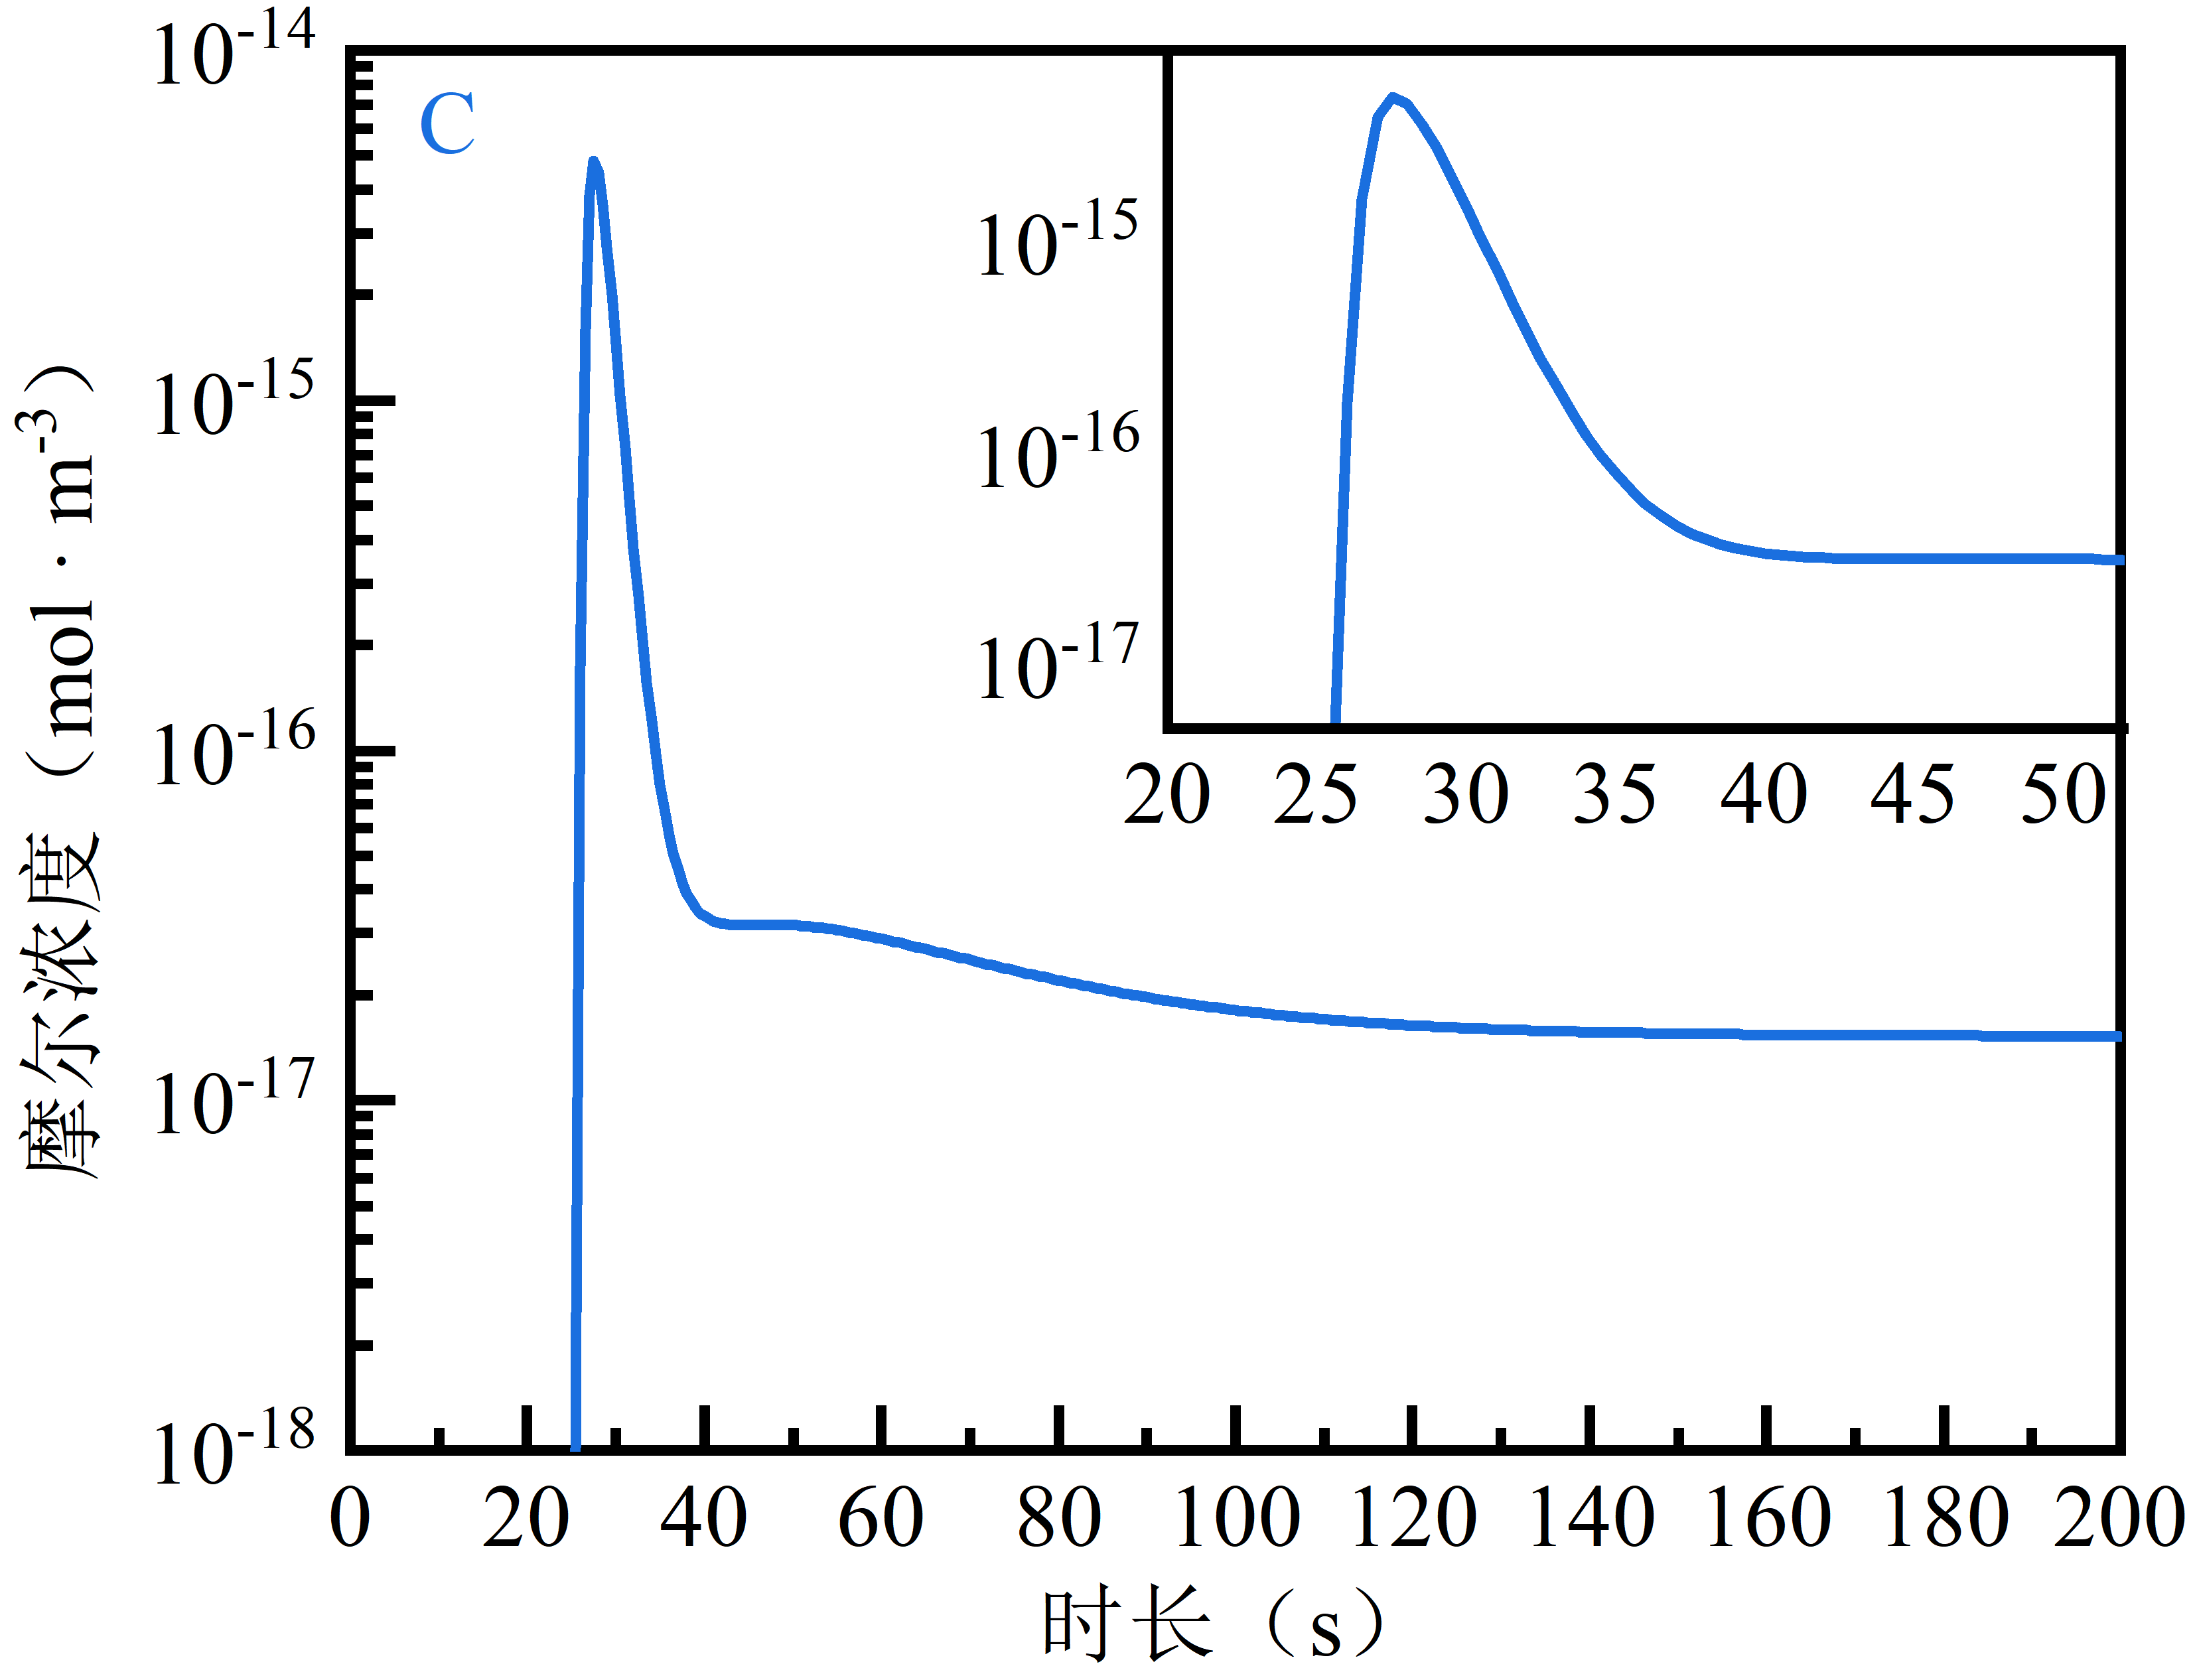
\includegraphics{pic/FLG_fluent_C_molConcen.png}
    }
    \subfloat[]{
        \label{fig:FLG_fluent_O_molConcen}
        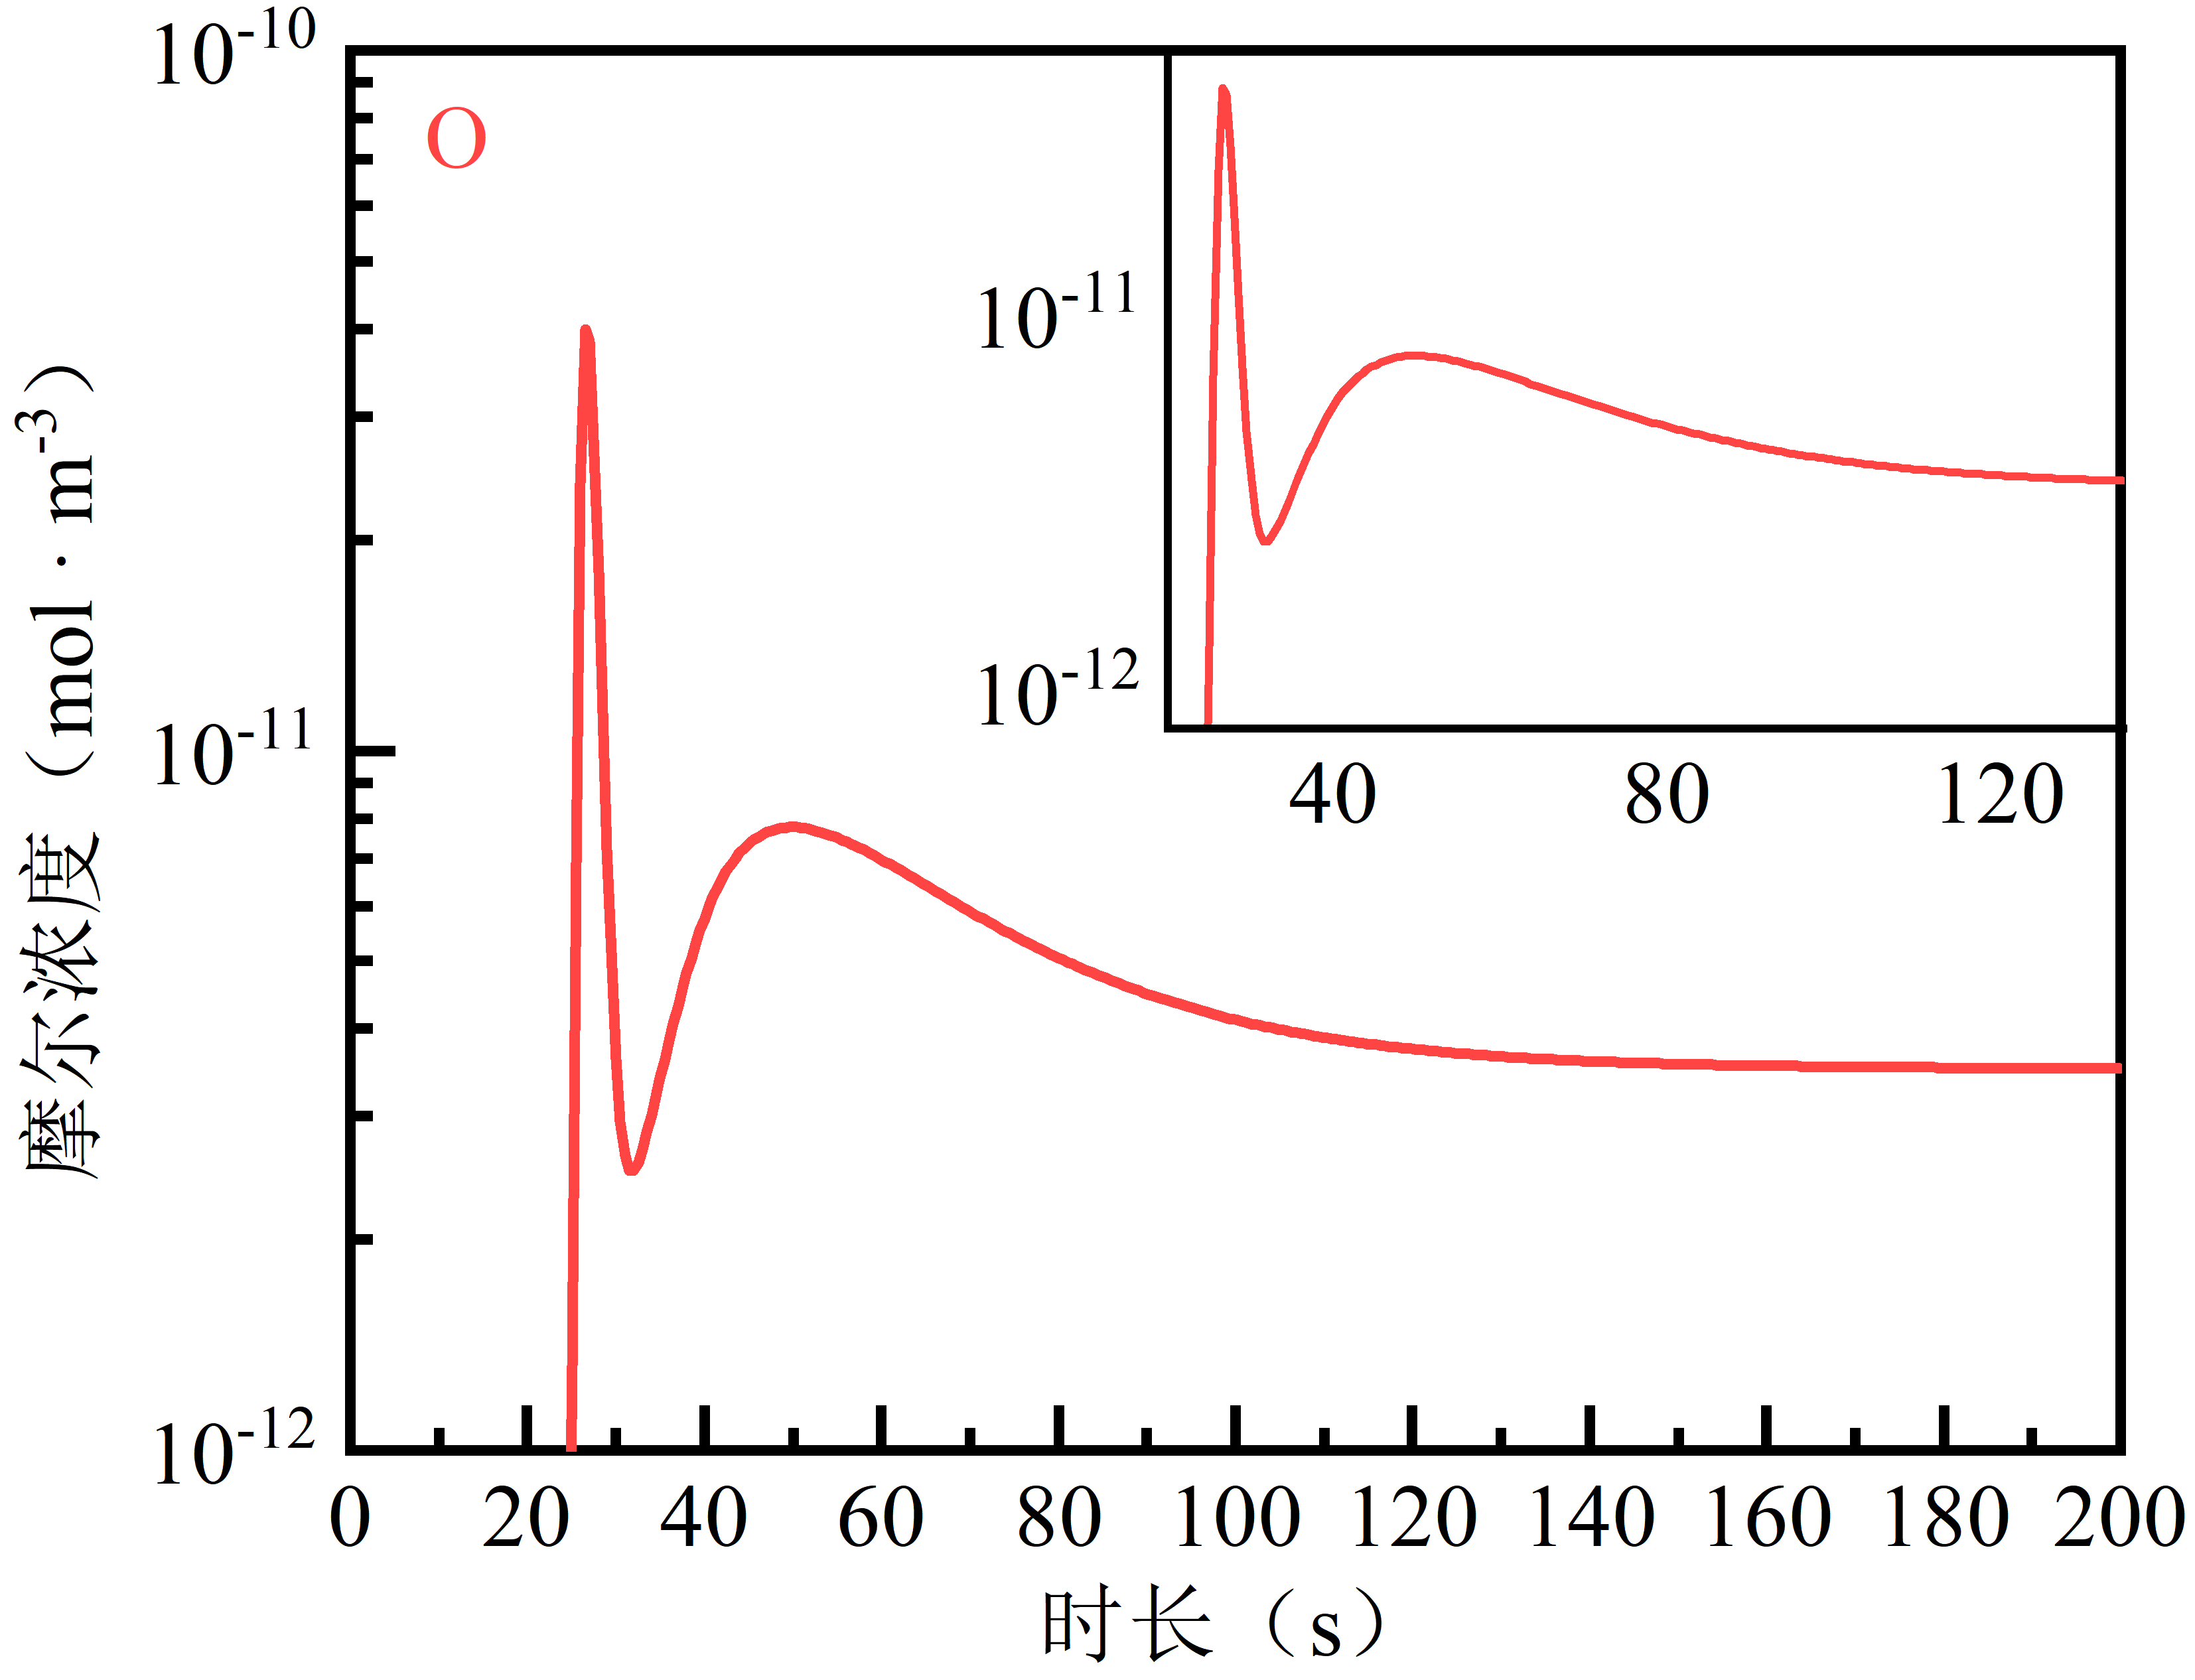
\includegraphics{pic/FLG_fluent_O_molConcen.png}
    }\\[-0.5ex]
    \subfloat[]{
        \label{fig:FLG_fluent_O-C_ratio}
        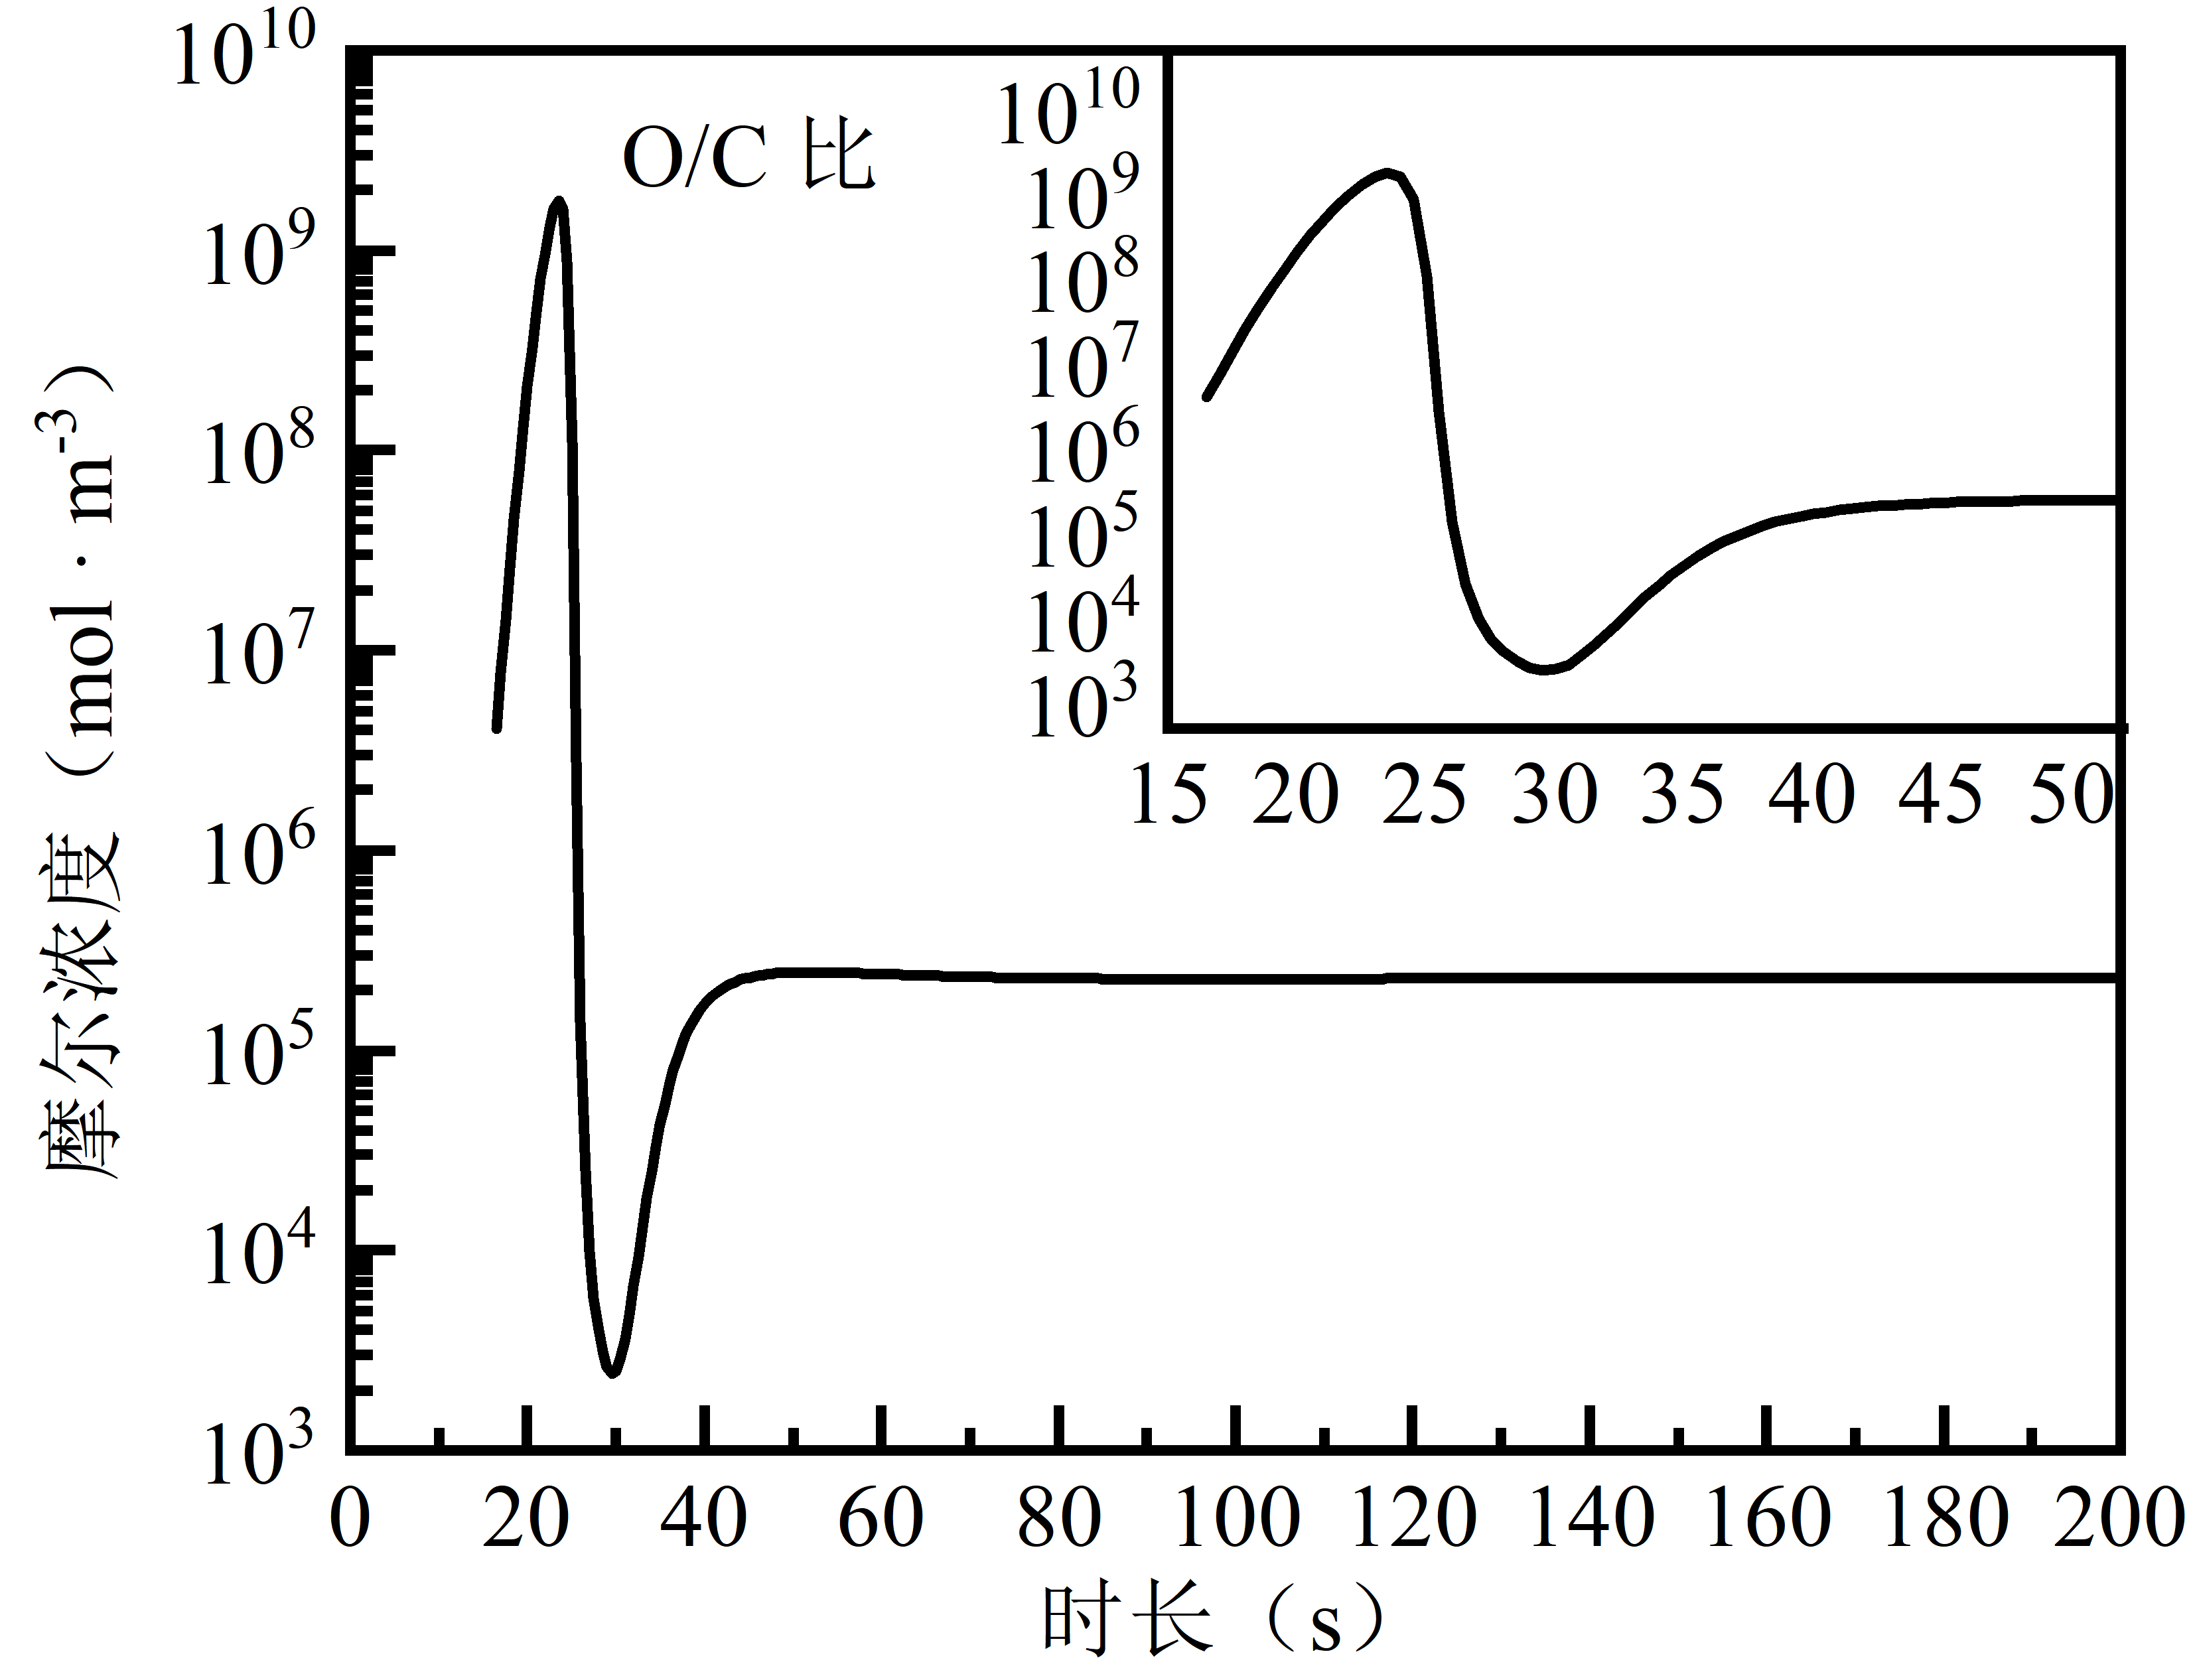
\includegraphics{pic/FLG_fluent_O-C_ratio.png}
    }
    \caption{化学气相沉积过程中石墨烯生长位点的化学组分随时间分布的浓度变化。(a)C自由基浓度(b)O自由基浓度(c)O/C比例。
    }
    \label{fig:FLG_fluent}
\end{figure}

本论文使用反应活性最高的C自由基和O自由基作为气相中直接参与石墨烯生长和蚀刻反应的代表反应物。可以看到在常压化学气相沉积的系统内,输入氧气后大约\SI{25}{\second}之后,在石墨烯生长位点开始有明显的甲烷分解反应发生。对于C自由基而言,由于氧气参与并促进甲烷的裂解反应,C自由基的浓度极速上升,最高浓度可达$\SI{4e-15}{\mole\per\cubic\metre}$。随后由于CO、CO2等碳氧化物的生成,C自由基的浓度迅速下降,并在约第\SI{40}{\second}后C自由基的浓度稳定在$\SI{1e-17}{\mole\per\cubic\metre}$附近。而对于O自由基,情况则更为复杂。在$\SI{25}{\second}$时,氧气经过气体输运到达石墨烯生长位点,被迅速加热开始分解成为氧自由基。此时氧自由基的最高浓度最高可达$\SI{3e-11}{\mole\per\cubic\metre}$。随后由于参与甲烷裂解和与氢气的化合反应,氧自由基的浓度下降至$\SI{2e-12}{\mole\per\cubic\metre}$并在产生震荡。氧自由基浓度震荡在约$\SI{50}{\second}$处到达最高值$\SI{8e-12}{\mole\per\cubic\metre}$并逐渐回落至$\SI{3e-12}{\mole\per\cubic\metre}$。考虑到在石墨烯的生长过程中,以C自由基和O自由基为代表的活性物质对于石墨烯的生长和蚀刻作用是同时进行的,因此本论文使用O/C比来考察化学气相沉积过程中,通入氩氧混合气后生长气氛中的化合物达到平衡状态所需的时间(图\ref{fig:FLG_fluent_O-C_ratio})。可以看到,在O/C比在通入氩氧混合气的第\SI{45}{\second}后就基本趋于稳定。考虑到实验中生长多层石墨烯通常需要几十分钟乃至几个小时的时间,因此可以认为在生长气氛中引入氧气的情况下,石墨烯生长、蚀刻反应所涉及的化学气氛均已达到稳态。由此,本论文更加快速高效对生长气氛进行稳态模拟。

图\ref{fig:FLG_chemkin}展示了通入不同流量的氧气情况下石墨烯生长位点的化学组分浓度情况。为了探究前驱体中不同氧气含量对多层石墨烯生长的影响,本论文考察了氩氧混合气输入的流量从$\SI{0}{SCCM}$ 到$\SI{500}{SCCM}$时,石墨烯生长气氛中的气相化学反应情况。

\begin{figure}[htb]
    \subfloat[]{
        \label{fig:FLG_chemkin_full}
        \includegraphics[width=0.48\textwidth]{pic/FLG_chemkin_full.png}
    }
    \subfloat[]{
        \label{fig:FLG_chemkin_part}
        \includegraphics[width=0.48\textwidth]{pic/FLG_chemkin_part.png}
    }
    \caption{生长环境中化学组分浓度分布随着通入氧气流量大小的变化情况。(a)模拟中涉及的所有化合物的浓度分布情况;(b)石墨烯蚀刻物质与生长物质的浓度分布情况}
    \label{fig:FLG_chemkin}
\end{figure}

整体来看,随着通入氧气流量的上升,甲烷的裂解程度也随之上升。甲烷与氧气反应生成大量的一氧化碳和二氧化碳以及种类众多的碳氢氧化合物。而碳氢化合物的浓度随着氧气通入流量的上升呈现出先上升后下降的趋势。氢气的浓度随着更多氧气的通入逐渐下降,但活性氢原子的浓度保持在一个非常稳定的区间。
为了简化分析,在氢-氧-甲烷反应所涉及的所有物质中,本论文主要关注那些能够蚀刻石墨烯以及能够为石墨烯生长提供碳源的化合物(图\ref{fig:FLG_chemkin_part})。其中,在本章中所考虑的蚀刻物质包括氧自由基、氢氧化物和氧气,生长物质包括活性炭自由基,碳氢化合物等。

对于蚀刻物质,本论文发现随着氧气通入量的上升,O、OH以及$\cemb{HO2}$的浓度急剧上升。以氧自由基为例,活性氧自由基的浓度在氩氧混合气的输入流量为$\SI{5}{SCCM}$时约为$\SI{2e-15}{}$。在氩氧混合气的输入流量为$\SI{500}{SCCM}$时,氧自由基在气氛中的浓度提升至$\SI{3e-2}{}$,大约提升了三个数量级。而对于$\cemb{OH}$和$\cemb{HO2}$,二者的浓度随着氩氧混合气的输入流量的上升也有两到三个数量级的浓度提升。

而气氛中的生长物质随着氧气通入量的上升呈现出了了非单调的变化。氧气能够促进甲烷的裂解反应,因此气氛中的C和CH的浓度得以缓慢上升,作为甲烷裂解反应物和中间产物的$\cemb{CH4}$,$\cemb{CH3}$,$\cemb{CH2}$则缓慢下降。而其他碳氢化合物在氧气通入量逐渐上升的情况下大部分呈现出先上升后下降的浓度趋势。
\subsection{氧对多层石墨烯的穿透蚀刻机制}
\label{subsec:FLG_Oetch}

考虑到蚀刻物质中$\cemb{O}$、$\cemb{OH}$、$\cemb{HO2}$以及$\cemb{O2}$等物质都对石墨烯具有一定的蚀刻作用,且各蚀刻物质之间的浓度较为接近。为了探究石墨烯在含氧化学气相沉积环境下的蚀刻过程,本论文引入氧原子的化学势$\muO{}$来代表生长气氛中蚀刻物质的整体反应活性。因此,化学势$\muO{}$的变化范围为$\halfEOm$ 至 $\EOa$,对应于氧原子在氧气分子($\cemb{O2}$)内的能级水平和氧原子在氧自由基($\cemb{O}$)中的能级水平。随着在蚀刻石墨烯的反应中涉及的高活性蚀刻物质(如氧自由基O)浓度的上升,化学势$\muO{}$逐渐上升并接近$\EOa$,同时伴随着更多的石墨烯被蚀刻。

随后,利用密度泛函理论,在$\muO{}$的框架内计算了氧原子蚀刻石墨烯的反应能$\rm{\Delta} \it E$。
\begin{equation}
    \rm{\Delta} \it E = E_{\rm product} - E_{\rm initial} - \muO{}
\end{equation}
其中,$E_{\rm product}$和 $E_{\rm initial}$分别为各反应步骤中生成物和反应物的能量。

在以铜为衬底的化学气相沉积石墨烯生长法中,当铜的表面被单层的石墨烯覆盖满后,石墨烯多层的生长由于自限制效应而趋近于停止。此时的石墨烯-\cemb{Cu}衬底界面处存在大量的游离碳。这些游离碳在石墨烯-\cemb{Cu}衬底的界面处扩散,成核,形成少量的石墨烯多层点。从热力学的角度看,石墨烯多层点的大小于游离碳的浓度$\Cdis$处于平衡状态。当游离碳的浓度$\Cdis$上升时,处于石墨烯-\cemb{Cu}衬底的界面处的石墨烯多层点的成核密度上升、面积扩大。当游离碳的浓度$\Cdis$下降时,石墨烯多层点开始分解,面积缩小。

从密度泛函理论的计算结果来看(图\ref{fig:FLG_DFT_Oetch}),无论有无游离碳,氧原子都可以在石墨烯上吸附,并且吸附的反应能相近。对于氧气来说,由于在石墨烯上吸附需要进行裂解,因此当$\muO{}=\halfEOm$时,氧原子在界面游离碳上方的石墨烯上的吸附能约为$\SI{-0.35}{\electronvolt}$,在纯石墨烯的表面吸附能约为$\SI{-0.28}{\electronvolt}$。而对于氧自由基而言,其可以在石墨烯上直接吸附,相应的吸附步骤的反应能也会下降很多。计算显示当$\muO{}=\EOa$时,氧原子在界面游离碳上方的石墨烯上的吸附能约为$\SI{-3.63}{\electronvolt}$,在纯石墨烯上的吸附能约为$\SI{-3.56}{\electronvolt}$。

\begin{figure}[htb]
    \includegraphics{pic/FLG_DFT_Oetch.png}
    \caption{
        石墨烯多层以及石墨烯单层在含氧环境下的蚀刻。$\muO{eg}$为氧蚀刻石墨烯单层时的平衡化学势。图中,铜原子、碳原子、氧原子、氢原子分别使用橙色、灰色、红色和白色标识。
    }
    \label{fig:FLG_DFT_Oetch}
\end{figure}

氧原子吸附在石墨烯上后,和石墨烯表面的碳原子发生反应,生成非常稳定的\cemb{CO}。同时,当界面游离碳存在的时候,石墨烯上被氧原子蚀刻而成的碳空位能够被游离碳修复。这种类似于交换作用的机理使得环境中的氧原子能够通过蚀刻石墨烯单层的方式减少界面游离碳的浓度$\Cdis$,进而导致石墨烯多层点的蚀刻。计算显示,氧原子在游离碳上方的石墨烯位点蚀刻石墨烯形成\cemb{CO}的反应在所有考虑的氧原子能级$\muO{}$下都为放热反应,在$\muO{}=\halfEOm$时反应能$\rm{\Delta} \it E=\SI{-2.59}{\electronvolt}$;在$\muO{}=\EOa$时反应能$\rm{\Delta} \it E=\SI{-5.87}{\electronvolt}$。这意味着即使环境中只存在少量的氧气($\muO{} \approx \halfEOm$),生长气氛中的氧就能够通过蚀刻石墨烯单层和游离碳的交换作用对界面处的石墨烯多层进行蚀刻。

当界面处的石墨烯多层被完全蚀刻、游离碳的浓度$\Cdis$也被环境中的氧消耗至零时,氧气与石墨烯单层表面碳原子反应产生的碳空位无法被修复,在石墨烯表面产生高能态的单空位缺陷(Single vacancy, SV)。空位缺陷的产生会极高地抬升氧原子蚀刻石墨烯单层的反应能。导致的结果是只有当环境中氧原子的能级水平提高至接近氧自由基的能级$\EOa$时,蚀刻反应才能够从吸热反应变为放热反应,此时的$\muO{} \leqslant  \muO{eg}  $,才能够进一步对石墨烯单层进行蚀刻。$\muO{eg}$为氧蚀刻石墨烯单层时的平衡化学势。因此,对于石墨烯单层的蚀刻需要通入更高流量的氧气以抬高生长气氛中氧的反应活性。

\subsection{氧对多层石墨烯的穿透生长机制}
\label{subsec:Opene}
在第\ref{subsec:FLG_gasPhase}章中,本论文模拟了引入不同流量的氧气的情况下石墨烯生长位点的化合物浓度分布情况。对于生长物质,本论文发现\cemb{C2H2}分子的摩尔浓度相比于其他的生长物质的浓度高出多个数量级。因此本论文考虑将\cemb{C2H2}分子作为本章的主要研究对象,探究其对于石墨烯多层生长的影响。

首先,本论文通过密度泛函理论计算,研究\cemb{C2H2}在石墨烯表面的吸附机理(图\ref{fig:FLG_DFT_C2H2toCHO})。对于无氧生长气氛下的石墨烯,计算结果显示\cemb{C2H2}在其上的吸附反应是吸热的,吸附能为$\SI{0.11}{\electronvolt}$。
这一结果和已有的研究吻合\citing{RN248-2014}。吸热的吸附过程说明\cemb{C2H2}较难在纯石墨烯上吸附,因此也较难对石墨烯多层点的生长产生作用。在有氧的生长气氛下,在\ref{subsec:FLG_Oetch}章中,本论文已经证明了生长气氛中的氧在能量上很容易在石墨烯的表面形成吸附氧原子。当石墨烯的表面存在吸附氧原子时,进一步的计算显示气氛中的\cemb{C2H2}可以与吸附氧原子反应,在石墨烯的表面形成\cemb{C2H2O}。这一步骤的反应能下降为$\SI{-1.54}{\electronvolt}$。随后,石墨烯表面吸附的\cemb{C2H2O}能够进一步和氧反应,形成更为稳定的\cemb{C2H2O2}。\cemb{C2H2O2}在石墨烯的表面可以分解成为两个分离的\cemb{CHO},进一步降低体系能量。在反应过程中,仅有\cemb{C2H2O2}分解为石墨烯表面相邻的\cemb{CHO}(图\ref{fig:FLG_DFT_C2H2toCHO},G-2HCO)过程中有小至$\SI{0.027}{\electronvolt}$的反应能上升,其余过程均为放热反应。因此可以在生长气氛中引入氧气的情况下,气氛中的\cemb{C2H2}可以大量的在石墨烯的表面吸附、分解成为同样吸附在石墨烯表面的\cemb{CHO}。

\begin{figure}[htb]
    \includegraphics{pic/FLG_DFT_C2H2toCHO.png}
    \caption{氧辅助\cemb{C2H2}在石墨烯表面沉积、分解为\cemb{CHO}。图中,铜原子、碳原子、氧原子、氢原子分别使用橙色、灰色、红色和白色标识。}
    \label{fig:FLG_DFT_C2H2toCHO}
\end{figure}

先前的研究表明,碳自由基以及碳氢化合物(\cemb{CH_x})等物质能够通过穿透的方式,在已生长的石墨烯的下方生长石墨烯多层\citing{RN248-2014}。由于碳自由基在生长气氛中非常低的浓度,已经环境中较高的氢自由基浓度,本论文选择\cemb{CH}作为代表化合物考察碳自由基以及碳氢化合物在含氧的生长气氛下对于石墨烯的穿透生长作用。在图\ref{fig:FLG_DFT_CHpene}中,本论文计算了石墨烯表面吸附的\cemb{CH}在有氧和无氧的气氛下可能的穿透反应路线。计算结果显示在无氧的气氛下,\cemb{CH}能够很好得在石墨烯得表面吸附并且通过穿透作用形成界面游离碳原子($\rm G-C_{inter}-H$)。

\begin{figure}[htb]
    \includegraphics{pic/FLG_DFT_CHpene.png}
    \caption{含氧气氛下石墨烯表面\cemb{CH}的穿透反应过程。}
    \label{fig:FLG_DFT_CHpene}
\end{figure}

然而在有氧的情况下,在石墨烯表面吸附的\cemb{CH}会优先和氧原子结合,在石墨烯的表面形成非常稳定的\cemb{CHO}。这一反应的反应能比\cemb{CH}穿透作用的反应能低$\SI{1.03}{\electronvolt}$。氧的引入阻断了\cemb{CH}通过穿透作用生长石墨烯多层的路径,并将其变为在石墨烯表面吸附的\cemb{CHO}。而\cemb{CHO}在石墨烯表面的吸附同样也遇到了困难。计算显示由于\cemb{CHO}在石墨烯表面极高的稳定性,其进行穿透反应所需吸收的能量约为$\SI{1.05}{\electronvolt}$。即使在穿透了碳原子后,残留的\cemb{OH}官能团与气氛中的\cemb{H}反应形成水蒸气也仍旧比\cemb{CHO}在石墨烯上吸附的能量要高。

\begin{figure}[htb]
    \includegraphics{pic/FLG_DFT_Odefect.png}
    \caption{\cemb{Cu}衬底表面不同构型的氧缺陷的形成能。图中,铜原子、碳原子、氧原子、氢原子分别使用橙色、灰色、红色和白色标识。}
    \label{fig:FLG_DFT_Odefect}
\end{figure}

在含氧的生长气氛下,\cemb{Cu}衬底可能产生氧缺陷。而\cemb{Cu}衬底表面的氧缺陷可能会对\cemb{CHO}在石墨烯表面的穿透作用产生影响。为了简化后续计算,本论文首先对不同构型的氧缺陷进行形成能计算。如图\ref{fig:FLG_DFT_Odefect}所示,本论文主要考虑\cemb{Cu}衬底表面氧的三种简单的点缺陷,分别为\chinesecolon 填隙氧原子缺陷\cemb{O_{i}}、单氧原子替位缺陷\cemb{O_{Cu}}以及双氧原子替位缺陷\cemb{2O_{Cu}},其中替位缺陷均为替换单个铜原子。形成能的计算使用$E_{\rm f}=E_{\rm Cu}^{\rm defect}+{\rm n_{Cu}}E_{\rm Cu}^{\rm bulk}-\frac{1}{2}{\rm n_{O}}E_{O_{2}} - E_{\rm Cu}^{\rm perfect}$。其中$E_{\rm Cu}^{\rm defect}$和$E_{\rm Cu}^{\rm perfect}$为缺陷\cemb{Cu}衬底和完美\cemb{Cu}衬底的能量;$E_{\rm Cu}^{bulk}$和$E_{O_{2}}$为块体铜和氧气的能量;${\rm n_{Cu}}$和${\rm n_{O}}$为缺陷反应中涉及的铜原子和氧原子的数量。计算结果显示三种点缺陷的形成能均为负值,形成能最低的单氧原子替位缺陷\cemb{O_{Cu}}的计算值为$\SI{-1.21}{\electronvolt}$。因此,本论文认为在生长了石墨烯的情况下,\cemb{Cu}衬底的表面仍然很容易形成氧原子缺陷。计算得到的形成能最低的氧缺陷构型为双氧原子替位缺陷\cemb{2O_{Cu}},其形成能为$\SI{-1.94}{\electronvolt}$。在后续的计算中,本论文使用双氧原子替位缺陷\cemb{2O_{Cu}}作为主要研究对象,考察\cemb{CHO}在石墨烯表面的穿透作用。

\begin{figure}[htb]
    \includegraphics{pic/FLG_DFT_CHOpene.png}
    \caption{\cemb{Cu}衬底上不同位点的石墨烯表面吸附的\cemb{CHO}的穿透反应过程。图中,铜原子、碳原子、氧原子、氢原子分别使用橙色、灰色、红色和白色标识。穿透进入界面的游离碳原子使用蓝色标识。}
    \label{fig:FLG_DFT_CHOpene}
\end{figure}

在图\ref{fig:FLG_DFT_CHOpene}中,本论文绘制了\cemb{Cu}衬底上不同位点的石墨烯表面吸附的\cemb{CHO}的穿透反应过程,包含无氧缺陷的原生位点以及双氧原子替位缺陷\cemb{2O_{Cu}}的氧缺陷位点。对比\cemb{CHO}在铜表面原生位点的石墨烯穿透反应,铜表面的氧缺陷位点对于游离碳有更高的亲和性,消除了\cemb{CHO}穿透石墨烯的上升势。具体而言,在\cemb{Cu}衬底的氧缺陷位点,吸附在石墨烯表面的\cemb{CHO}的穿透反应能为$\SI{-1.27}{\electronvolt}$。同时,在穿透反应完成后,石墨烯上残留的\cemb{OH}官能团能与气氛中的氢反应,进一步降低体系能量并且释放处氧缺陷位点,使得\cemb{CHO}在氧缺陷位点的穿透反应能够持续不断的进行。虽然穿透反应过程中的交换作用使得原石墨烯单层表面的碳原子进入界面成为游离碳,但是\cemb{CHO}对于石墨烯表面的\cemb{Cu}衬底位点选择性穿透使得在界面处生长的石墨烯多层的碳原子主要来源于含氧气氛内的碳源。倘若穿透反应能够在石墨烯单层表面的任意位点进行,那么由于石墨烯表面吸附分子的扩散作用,穿透进入界面的游离碳并成核生长为石墨烯多层点的碳原子应该主要来自于原石墨烯单层的碳原子。因为在随机作用下,只有很少的位点会产生多层点穿透的现象。如果穿透反应对于\cemb{Cu}衬底的氧缺陷位点具有选择性,氧缺陷位点处产生的穿透通道使得大部分的穿透都在氧缺陷位点上方进行,由此会产生在石墨烯单层表面多层点穿透的情况,如此一来穿透进入界面的游离碳并成核生长为石墨烯多层点的碳原子则主要来源于生长气氛。因此,通过同位素标记法区别原石墨烯单层表面的碳原子以及含氧气氛中的碳原子,可以通过实验验证穿透的机制的选择性\citing{RN1262-2021}。

\subsection{氧辅助多层石墨烯蚀刻生长模型及模式切换相图}
综合考虑氧气的引入对于界面处石墨烯多层蚀刻和生长的影响,可以发现氧对二者均有促进作用。对于氧蚀刻反应,根据通入的氧流量的不同导致生长气氛中氧的化学势$\muO{}$的变化,本论文将蚀刻反应分为两个阶段。在第一个阶段中,只有界面处的游离碳通过与石墨烯单层的交换左右,被气氛中的氧蚀刻,导致界面游离碳的浓度$\Cdis$下降,界面石墨烯多层点减少。第二个阶段是当通入的氧流量足够高时,氧的化学势超过蚀刻石墨烯单层的平衡化学势$\muO{} \geqslant \muO{eg}$,导致石墨烯单层开始被氧蚀刻。可以将氧对石墨烯的蚀刻作用总结为以下化学表达式\chinesecolon
\begin{equation}
    \label{chemeq:OetchReaction}
    \begin{split}
        \cemb{C($\rm dis.$) + O($\rm ads.$) &->[graphene] CO(g)} \\
        \cemb{C(graphene) + O($\rm ads.$) + 2H &->[\vphantom{graphene}] CO(g) } \mbox{ only if $\muO{} \geqslant \muO{eg}$}
    \end{split}
\end{equation}
根据\ref{subsec:Opene}章,氧辅助的穿透反应可以写为\chinesecolon
\begin{align}
    \label{chemeq:OpeneReaction}
    \cemb{C2H2(g) + 2O($\rm ads.$) + 2H(g) ->[graphene][Cu oxygen defect] 2C(adlayer) + H2O(g)}
\end{align}

根据反应式\ref{chemeq:OetchReaction},可以写出理想状况下的蚀刻速率\chinesecolon
\begin{equation}
    \RateV{e}{}=\rule[0ex]{0ex}{8ex}\left\{
        \begin{array}{ll}
        \smash[t]{\overbrace{\RateK{e}{dis.}\Cdis\Oads}^{\mathclap{{\mbox{\normalsize $\RateV{e}{dis.}$}}}}} & \mbox{}  \\
        \smash[b]{\RateK{e}{dis.}\Cdis\Oads+\RateK{e}{g}\Oads} & \mbox{for $\muO{} \geqslant \muO{eq}$} 
        \end{array}\right.
        %\begin{array}{ll}\hline
        %    \rule[10ex]{1ex}{4ex}\\\hline
        %\end{array}
\end{equation}
和穿透速率\chinesecolon
\begin{equation}
    \RateV{g}{}=\RateK{g}{}\cemb{[C2H2][H2]^2}\Oads^2
\end{equation}
其中,$\RateK{e}{dis.}$、$\RateK{e}{g}$和$\RateK{g}{}$分别为游离碳蚀刻,石墨烯单层蚀刻,石墨烯多层生长的反应常数。$\Cdis$、$\cemb{[C2H2]}$、$\cemb{[H]}$和$\Oads$代表界面游离碳、$\cemb{C2H2}$化合物、$\cemb{H}$自由基以及石墨烯上吸附氧的浓度。

考虑蚀刻石墨烯多层时,氧原子对于的界面游离碳消耗\chinesecolon
\begin{equation}
    \RateV{e}{dis.}=\RateK{e}{dis.}\left(\Cdis-\RateV{e}{dis.}\right)\Oads
\end{equation}
其中,$t$为反应的时间。随着氧原子对石墨烯多层蚀刻的进行,界面游离碳逐渐被消耗,$\Cdis$的下降同时降低了石墨烯多层蚀刻反应的速率。将反应速率$\RateV{e}{dis.}$对反应时间$\ReactTime{O}{}$积分并取平均,可以得到$\ReactTime{O}{}$时间段内的氧气对游离碳的平均蚀刻反应速率\chinesecolon
\begin{equation}
    \overline{\RateV{e}{dis.}}=\frac{\int_{0}^{\ReactTime{O}{}} \RateV{e}{dis.} \,dt }{\ReactTime{O}{}}=\frac{\int_{0}^{\ReactTime{O}{}} \frac{\RateK{e}{dis.}\Cdis\Oads}{\RateK{e}{dis.}\Oads \ReactTime{}{} + 1} \,dt}{\ReactTime{O}{}}
\end{equation}
而对于生长反应,$\cemb{CHO}$在石墨烯表面的选择性吸附使得生长反应速率$\RateV{g}{}$存在一个由\cemb{Cu}衬底表面氧缺陷位点数量限制的上界。可以写出在氧缺陷处的穿透通道被饱和之前的生长反应的平均速率\chinesecolon
\begin{equation}
    \overline{\RateV{g}{}}=\frac{\int_{0}^{\ReactTime{O}{}} \RateV{g}{} \,dt }{\ReactTime{O}{}}= \frac{\int_{0}^{\ReactTime{O}{}} \RateK{g}{}\cemb{[C2H2][H2]^2}\Oads^2 \,dt }{\ReactTime{O}{}}
\end{equation}
在这些化合物的浓度中,$\cemb{[C2H2]}$和$\cemb{[H]}$本论文使用\ref{subsec:FLG_gasPhase}节中模拟出的相应化合物的稳态浓度数据。而对于$Odis$,虽然在\ref{subsec:FLG_gasPhase}章中的模拟证明生长环境中的化合物很快就达到了稳态平衡,但由于氧自由基($\cemb{O}$)较低的浓度以及氧分子($\cemb{O2}$)在石墨烯表面较低的吸附能。氧气的吸附过程可能会需要很长的一段时间才会达到饱和。为了获得$\Oads$在石墨烯多层生长过程中随时间的变化情况,本论文使用晶格随机顺序吸附模型(lattice random sequential adsorption model )对氧气以及氧原子在石墨烯表面的吸附进行模拟。

晶格随机顺序吸附模型中,本论文使用二维晶格对石墨烯进行模拟,每个晶格单元对应一个原胞大小的石墨烯。在模拟过程中,本论文考虑生长气氛中氧气分子($\cemb{O2}$)和氧自由基($\cemb{O}$)在石墨烯表面的沉积。根据密度泛函理论计算(表\ref{tab:FLG_RSA_coverage}),取$\cemb{O2}$和$\cemb{O}$在石墨烯表面吸附的饱和覆盖率分别为$1$和$1 / 4$。

\begin{table}
    \centering
    \caption{}
    \begin{tabular}{ccc}
        \toprule
        覆盖率  & $\cemb{O}$的吸附能(\si{\electronvolt}) & $\cemb{O2}$的吸附能(\si{\electronvolt}) \\
        \midrule
        1       & -4.50                                    & 0.43                                      \\
        $1 / 4$ & -4.95                                    & -0.026                                    \\
        \bottomrule
    \end{tabular}
    \label{tab:FLG_RSA_coverage}
\end{table}

同时,有别于氧自由基($\cemb{O}$)的直接吸附,氧气分子$\cemb{O2}$在石墨烯上的吸附的同时需要较高的能量进行进行裂解。本论文通过在氧气分子吸附的过程中添加$\SI{2.39}{\electronvolt}$的势垒来对这个裂解过程进行描述\citing{RN838-2012}。为了将随机吸附模拟过程中的模拟时间时长与实际通入氩氧混合气的时长进行对应,本论文根据气体的麦克斯韦-玻尔兹曼分布计算了氧自由基($\cemb{O}$)和氧气分子$\cemb{O2}$的碰撞频率,气氛中氧自由基($\cemb{O}$)和氧气分子$\cemb{O2}$的浓度也根据\ref{subsec:FLG_gasPhase}节中的模拟数据进行计算。

在图\ref{fig:FLG_RSA_Oadsorb}中,本论文计算了通入不同流量的氩氧混合气的情况下石墨烯上吸附的氧原子浓度$\Oads$随时间的变化情况。计算结果显示模拟得出的$\Oads$服从指数增长定律$\Oads\left(\it t\right)=\Oads\left(\it \infty \right)-\it De^{\it -\sigma t}$,和先前的研究一致\citing{RN837-1990,RN836-1991}。由于$\Oads$的指数形式,直接将$\Oads$带入计算$\overline{\RateV{e}{dis.}}$中的积分项为非初等函数。考虑到在实际的化学气相沉积生长过程中,氧原子在低浓度氧环境中需要花费数天甚至一个月的时间才能达到饱和吸附,远超本论文所考虑的生长时间范畴。而高浓度氧环境中会导致石墨烯被完全蚀刻,也不在本论文所关心的范围内。因此本论文将研究范围集中在氧原子吸附浓度$\Oads$的线性吸附区,这时$\Oads$相对于时间的变化关系可以简化为$\Oads\left(\it t\right)\approx \it D \sigma t$。

\begin{figure}[htb]
    \includegraphics{pic/FLG_RSA_Oadsorb.png}
    \caption{不同氩氧混合气通入流量下氧原子在石墨烯表面吸附浓度随时间的变化情况。}
    \label{fig:FLG_RSA_Oadsorb}
\end{figure}

为了确认$\Oads$线性简化是否会因为晶格随机顺序吸附模拟过程中所使用的屏蔽系数参数的变动而失效。如图\ref{fig:FLG_RSA_OabsorbPera}所示,本论文计算了在中等氧通量的情况下(氩氧混合气流量为\SI{100}{SCCM}),多种模拟参数组合下氧原子在石墨烯表面进行吸附模拟的结果。可以看到,氧气$\cemb{O2}$屏蔽系数的变化几乎无法传到至最后吸附浓度的变化。这可能是由于氧气较高的解离势垒导致尽管生长气氛中的氧气浓度较高,但氧气在石墨烯表面解离吸附在石墨烯上的能力仍然较弱。而对于氧自由基$\cemb{O}$,屏蔽系数由$1$变为$\frac{1}{2}$会降低吸附氧原子的浓度。但考虑到通常化学气相沉积法对石墨烯的生长过程通常在$\SI{10}{\hour}$以内\citing{RN1262-2021}。在这个时间范围之内,氧自由基$\cemb{O}$屏蔽系数的变化对吸附氧原子浓度的影响较小。同时也并不会影响吸附氧原子浓度在$\SI{10}{\hour}$之内随时间的线性增长关系。因此,本论文认为对氧原子吸附浓度$\Oads$使用$\Oads\left(\it t\right)\approx \it D \sigma t$进行简化并不会受模拟过程中屏蔽系数参数选取的影响。

\begin{figure}[htb]
    \includegraphics{pic/FLG_RSA_OabsorbPera.png}
    \caption{$\Oads\left(\it t\right)\approx \it D \sigma t$线性近似的晶格随机顺序吸附模拟参数稳定性测试}
    \label{fig:FLG_RSA_OabsorbPera}
\end{figure}

由此,可以计算通入$\ReactTime{O}{}$的氩氧混合气后,石墨烯的蚀刻平均速率为\chinesecolon
\begin{equation}
    \label{eq:FLG_avgVe}
    \overline{\RateV{e}{}}=
    \begin{cases}
        \frac{\Cdis_0 \log\left( 1+\RateK{e}{dis.}\Oads | \,_{t=\ReactTime{O}{}} \ReactTime{O}{} \right) }{\it 2 \ReactTime{O}{}}                                                        & \muO{} \langle \muO{eg}         \\
        \frac{\Cdis_0 \log\left( 1+\RateK{e}{dis.}\Oads | \,_{t=\ReactTime{O}{}} \ReactTime{O}{} \right) }{\it 2 \ReactTime{O}{}} + \frac{1}{2}\RateK{e}{g}\Oads| \,_{t=\ReactTime{O}{}} & \muO{} \geqslant \muO{eg}
    \end{cases}
\end{equation}
其中,界面游离碳的初始浓度$\Cdis_0$本论文取相应生长温度下碳的饱和蒸汽进行近似。$\Oads| \,_{t=\ReactTime{O}{}}$为氩氧混合气的时间为$\ReactTime{O}{}$时的石墨烯上的吸附氧原子浓度。

同样,也可以求得在\cemb{Cu}衬底氧缺陷产生的穿透通道饱和前,石墨烯的生长平均速率为\chinesecolon
\begin{equation}
    \label{eq:FLG_avgVg}
    \overline{\RateV{g}{}} =\frac{1}{3}\RateK{g}{}\cemb{[C2H2]}\cemb{[H]^2}\left(\Oads |_{\,\ReactTime{}{}=\ReactTime{O}{}} \right)
\end{equation}
式\ref{eq:FLG_avgVe}和式\ref{eq:FLG_avgVg}可以解释氧促石墨烯多层蚀刻和氧促石墨烯生长之间的反应速率的竞争对于石墨烯多层整体蚀刻、生长行为的影响。在图\ref{fig:FLG_model_avgV}中,本论文绘制了不同吸附氧原子浓度下,氧辅助石墨烯蚀刻、生长作用的平均反应速率。

\begin{figure}[htb]
    \subfloat[]{
        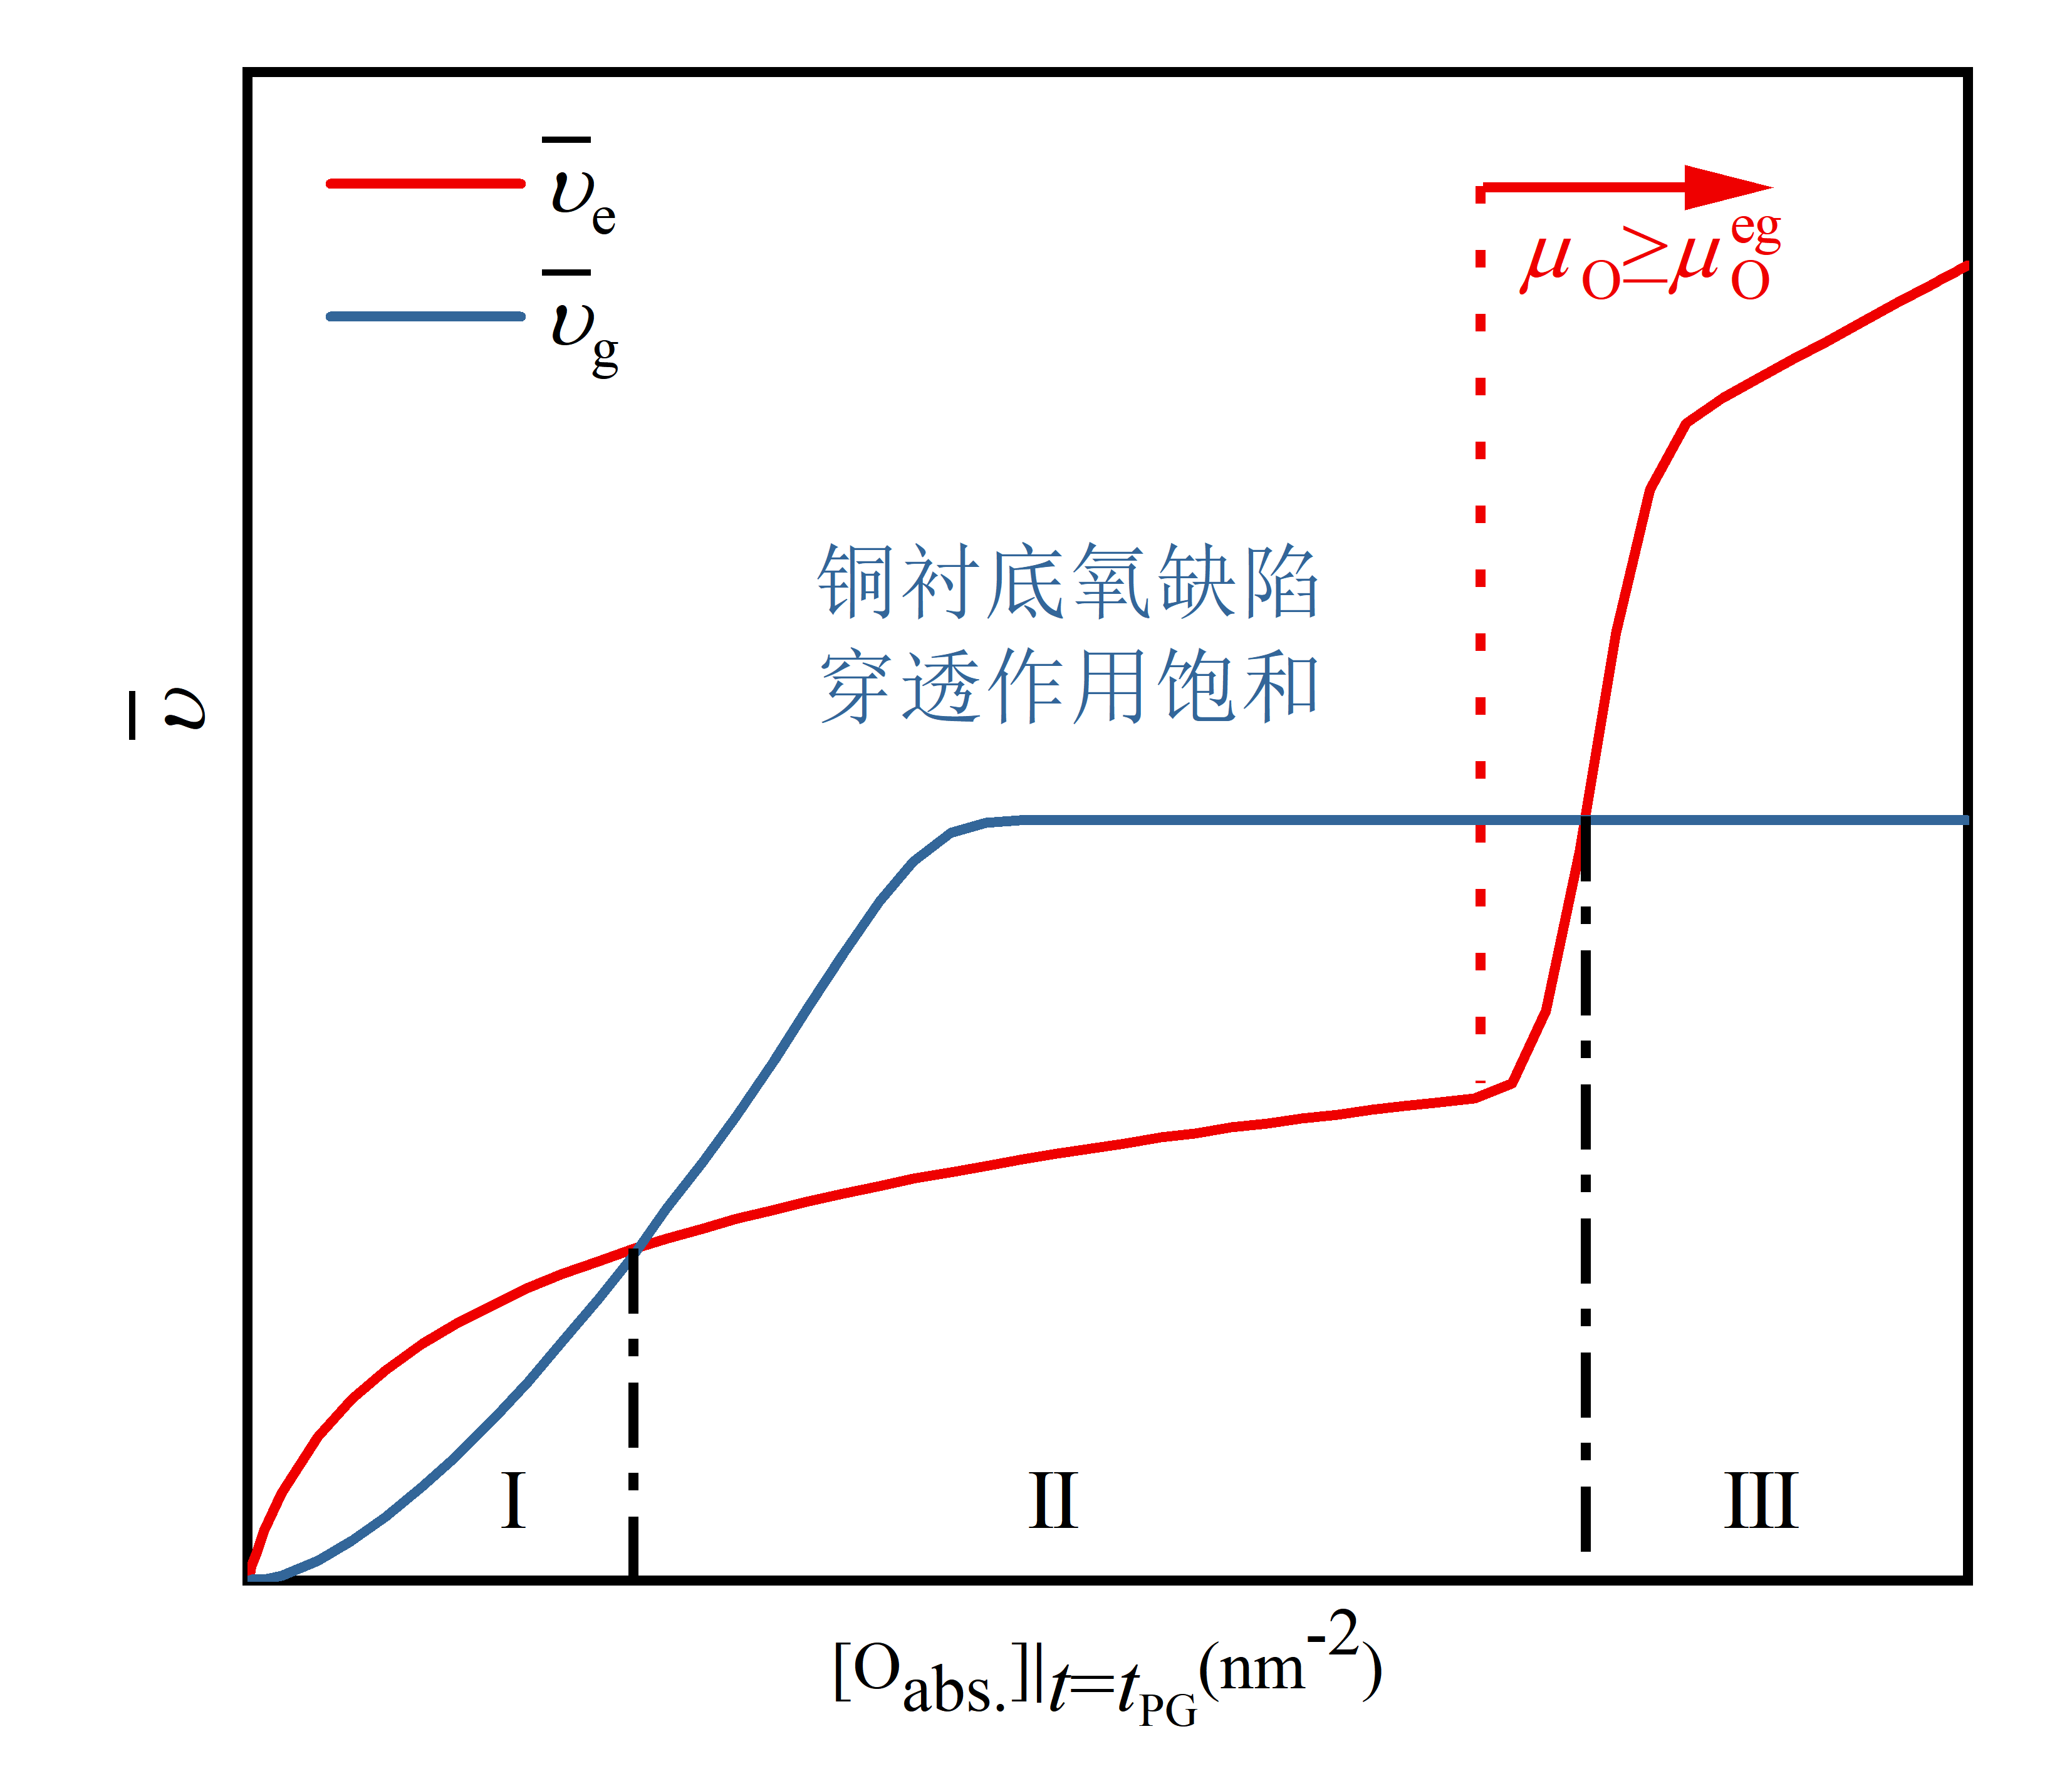
\includegraphics[]{pic/FLG_model_avgV.png}
        \label{fig:FLG_model_avgV}
    }
    \subfloat[]{
        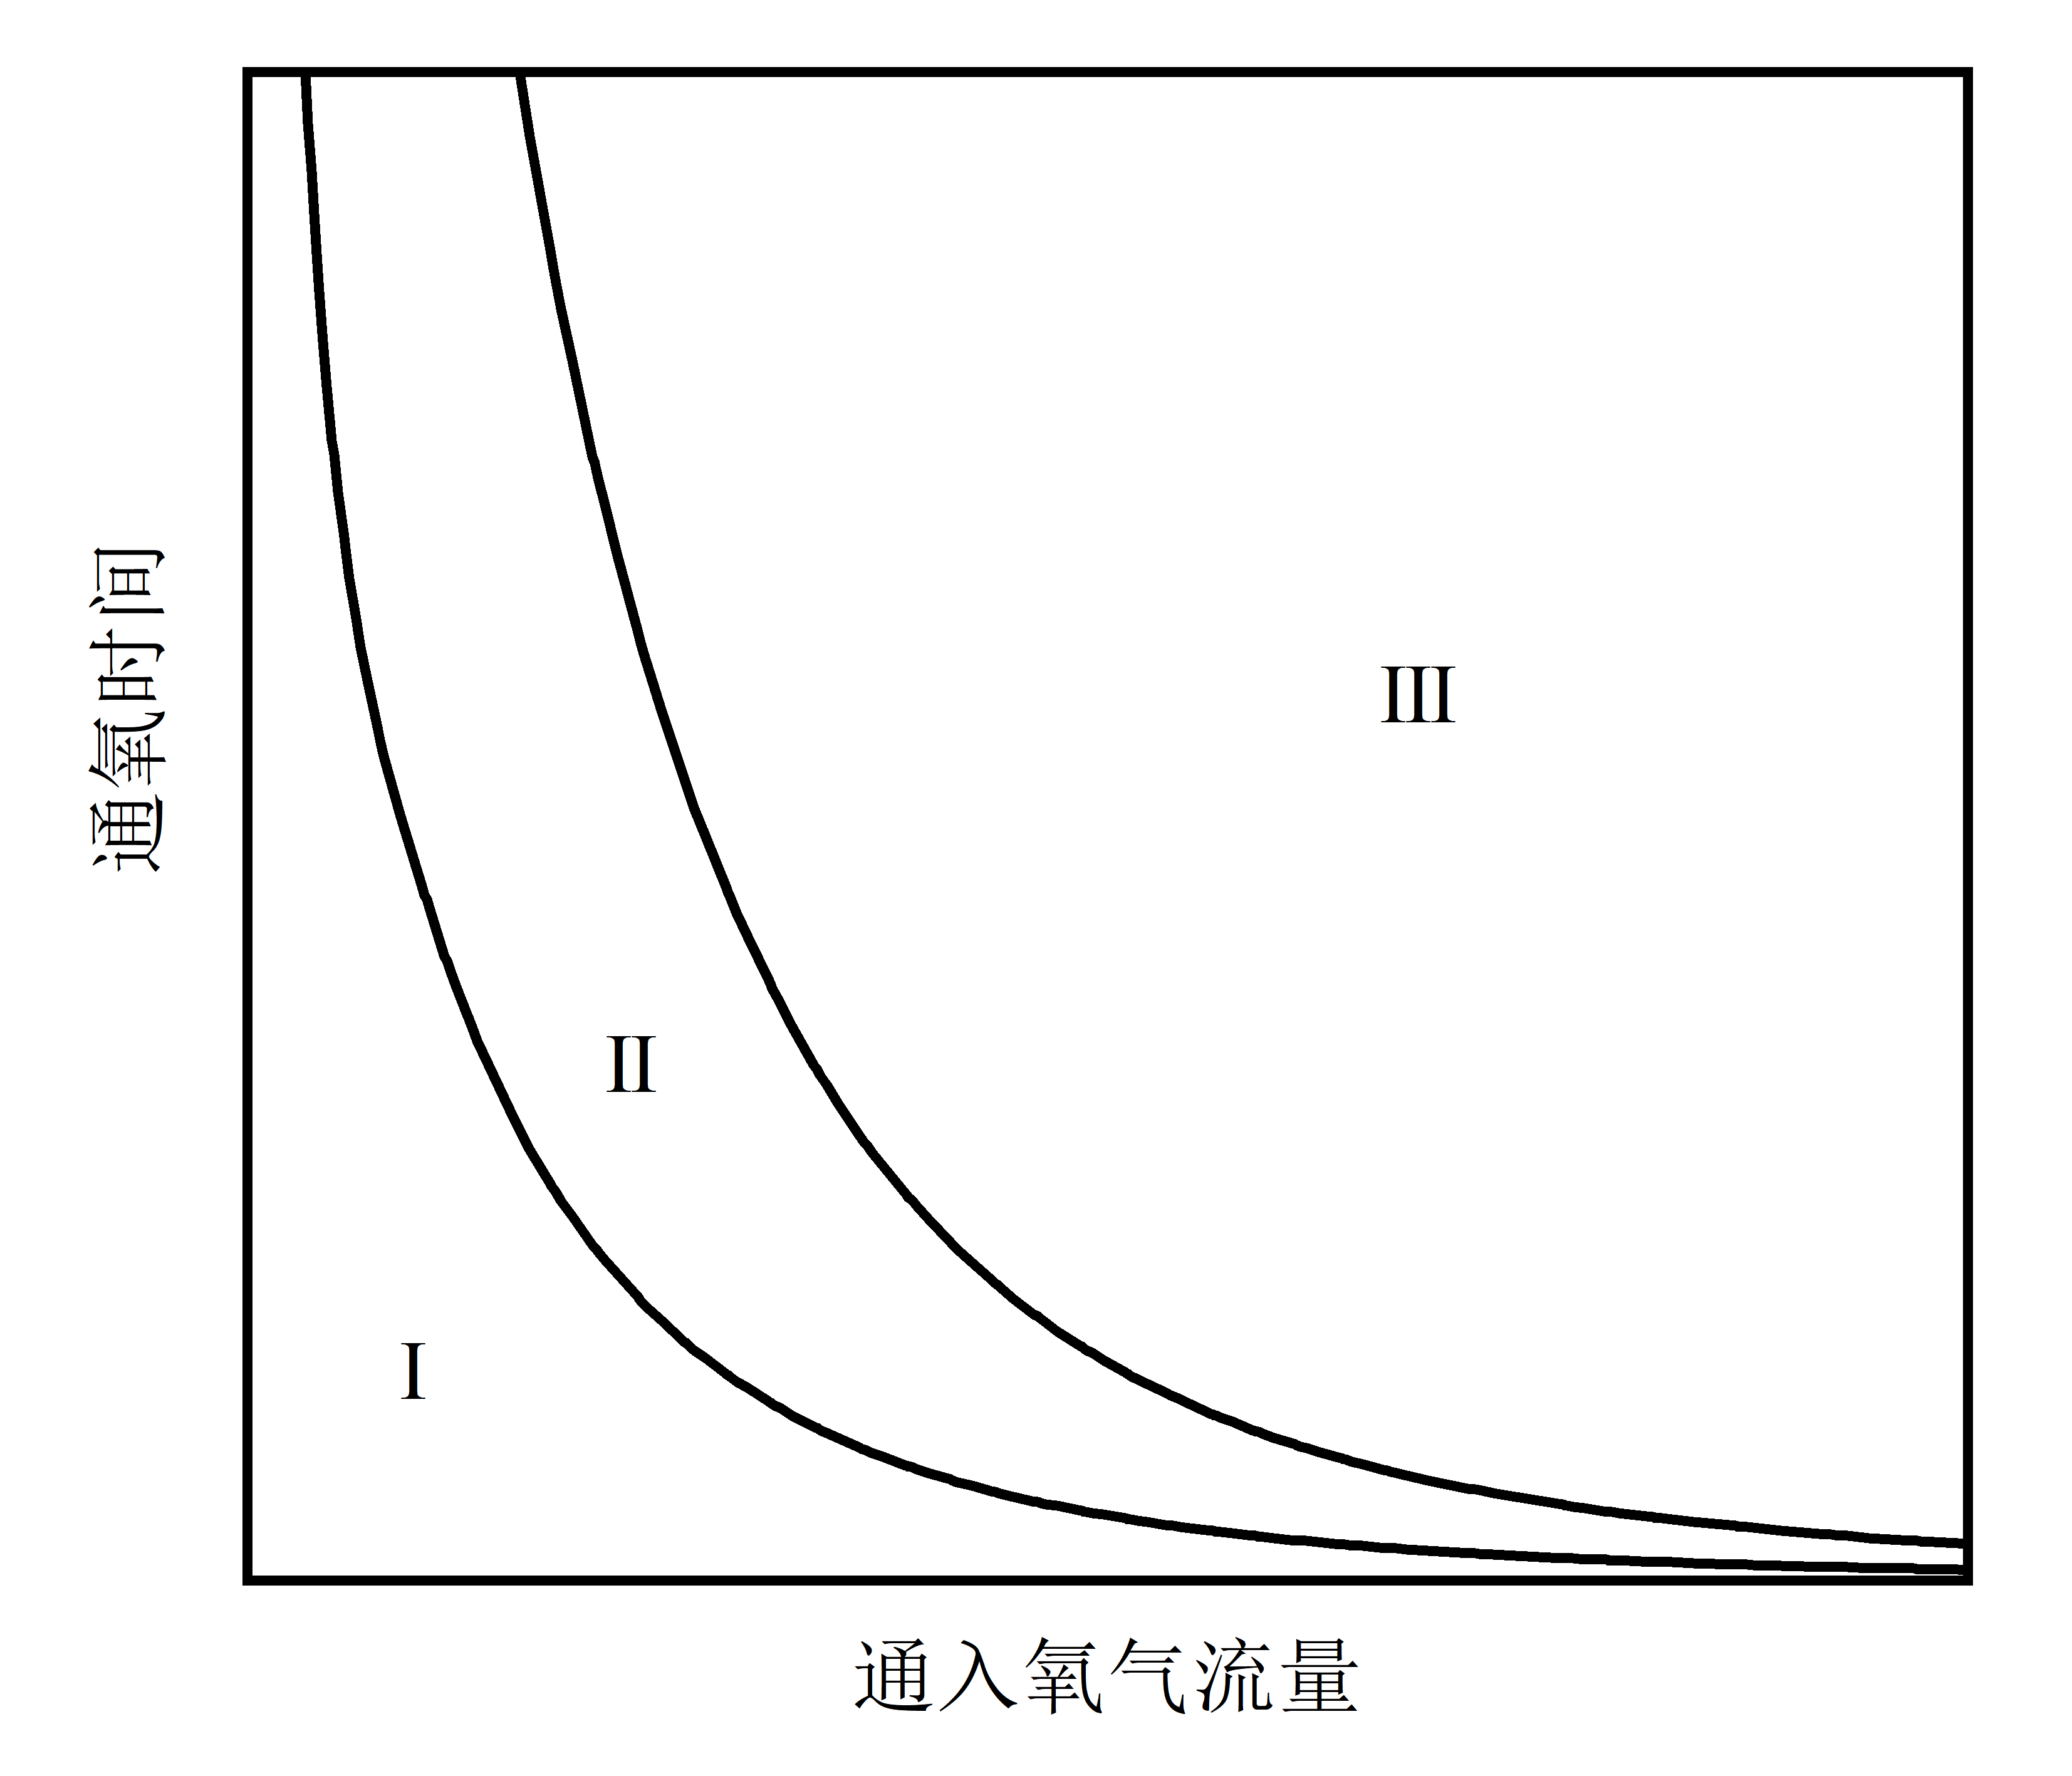
\includegraphics[]{pic/FLG_model_modePhase.png}
        \label{fig:FLG_model_modePhase}
    }
    \caption{氧辅助石墨烯蚀刻、生长作用及模式切换相图。(a)氧辅助石墨烯蚀刻、生长作用的平均反应速率;(b)氧辅助石墨烯蚀刻/生长模式切换相图。其中,模式I为石墨烯多层蚀刻、模式II为石墨烯多层生长、模式III为石墨烯蚀刻(包括石墨烯多层以及石墨烯单层)}
    \label{fig:FLG_model}
\end{figure}

图中的原点代表无氧气输入的情况,此时的石墨烯呈现出自限制的生长行为。当氧气引入生长气氛时,石墨烯表面吸附的氧原子浓度$\Oads$随着氧气通入量或者含氧气氛内反应时间的上升而上升。当吸附氧原子浓度$\Oads$较低时,石墨烯多层的蚀刻速率高于石墨烯多层的生长速率,石墨烯自限制生长下的少量多层点在氧原子的蚀刻作用下逐渐减少,整体表现出石墨烯多层蚀刻的行为(模式I)。当石墨烯表面吸附氧原子的浓度$\Oads$逐渐上升时,氧原子对于石墨烯表面的蚀刻反应速率由于界面游离碳浓度$\Cdis$的下降而放缓,$\cemb{CHO}$的穿透生长反应则随着$\Oads$的上升而继续加速。此时上升的$\Oads$导致石墨烯多层的生长速率高于被界面游离碳浓度不足所限制的石墨烯多层蚀刻速率,整体展现出石墨烯多层生长的行为(模式II)。当$\Oads$的浓度上升至氧的化学势$\muO{}$超过蚀刻石墨烯单层的平衡化学势$\muO{eg}$,气氛中的氧开始直接蚀刻单层石墨烯,导致石墨烯蚀刻反应的速率大幅上升,再次超过被穿透通道饱和所限制的石墨烯多层生长速率。此时石墨烯展现出再蚀刻的行为(模式III)。在模式III中,由于较高的氧活性,不仅石墨烯多层,较为稳定的石墨烯单层也会被高反应活性的氧反应。

\section{本章小结}
在本章中,本论文利用理论计算的方法研究了化学气相沉积生长石墨烯过程中衬底形貌和生长气氛对于的石墨烯生长行为的影响。研究表明衬底表面的台阶破坏了原衬底表面的对称性,为石墨烯的成核生长提供了优先生长位点和优先生长方向,使得石墨烯有机会在多晶铜的表面实现多点定向成核生长,有利于实现大面积石墨烯单晶生长的实现。而对于生长气氛的影响,本论文的研究显示氧的引入同时促进了石墨烯多层蚀刻和多层生长的反应。而氧气对石墨烯多层的蚀刻和穿透作用的相互竞争突破了原有\cemb{Cu}衬底上石墨烯生长的自限制作用,导致了石墨烯多层交替出现蚀刻和生长的现象,有利于实现石墨烯生长过程中的层数调控。

    \chapter{锑化铟的生长机理研究}
\section{引言}
\section{单层锑化铟生长过程及生长极性研究}
\section{双层锑化铟生长过程及生长极性研究}
\section{双层锑化铟生长及极性演化的物理机理研究}
\section{双层锑化铟生长极性相图}
    \chapter{二维材料异质结生长机理的研究}
\section{引言}
石墨烯作为经典的二维材料,由于独特的晶体结构和电子结构特性,在超导,量子计算、量子晶体管等方面具有独特的优势\citing{RN1068-2020,RN1071-2021,RN1065-2013,RN997-2007,RN1008-2015}。而要将石墨烯与现行集成电路使用的平面硅工艺兼容,需要将石墨烯转移到\cemb{SiO2}等绝缘衬底的表面。而石墨烯在\cemb{SiO2}等绝缘衬底表面通常以无序的状态存在,破碎的晶格使得石墨烯在这些绝缘衬底的表面难以完全发挥出理论上限。

而作为二维材料中的绝缘体,六方氮化硼\cemb{h-BN}在具有较大的带隙的同时也保有二维材料高质量面内结构的特点。趋近完美的二维晶体结构使得\cemb{h-BN}在禁带内具有极低的缺陷态密度以及较高的击穿电压。同时,\cemb{h-BN}与石墨烯之间的晶格失配只有\SI{2}{\percent},这使得\cemb{h-BN}非常适合搞高性能电子器件中替代\cemb{SiO2}作为石墨烯的衬底材料 \citing{RN959-2010}。这种将不同的二维材料纵向堆叠起来可以制成纵向异质结,层与层之间由较弱的范德华力或准范德华力连接。以二维材料所组成的异质结能够结合不同二维材料优异的物理特性,使得二维材料在多种新型器件中能够最大化的发挥其独特的优势。许多新奇的物理现象已经在石墨烯和\cemb{h-BN}的纵向堆叠而成的二维异质结被研究者所发现,如在外磁场下电子和磁场场强的霍夫斯塔特蝴蝶分型图像\citing{RN1286-2013, RN1287-2013, RN1285-2013}。同时,石墨烯/\cemb{h-BN}纵向二维异质结具有非常好的制备质量,石墨烯高度可调的物理特性,以及二者之间存在的周期性的摩尔超晶格。这些都使得石墨烯/\cemb{h-BN}纵向二维异质结成为了一个非常好的观测新奇量子现象的基础平台。

然而,虽然机械剥离的方式能够制备具有极高质量的石墨烯/\cemb{h-BN}纵向二维异质结,但受限于较低生产效率和高昂的合成成本,剥离的方式很难应用于大规模的二维材料的生产制备。而常用于大规模低成本制备石墨烯的化学气相沉积法通常需要\cemb{Cu}等金属衬底的催化作用的协助。由于\cemb{h-BN}对于甲烷等含碳前驱体裂解反应的催化活性远不及金属衬底,石墨烯在\cemb{h-BN}上直接生长的速率同样也远低于在金属衬底上的生长速率。因此,一些研究者试图通过增加前驱体裂解速率的方式提升纵向二维异质结的合成效率。例如,在2013年,研究者发现通过等离子体辅助的方式能够在低温的环境下在\cemb{h-BN}的表面生长石墨烯\citing{RN1289-2013}。在2015年,研究者通过添加作为气体催化剂的硅烷等方式,可以促进甲烷的裂解,提高石墨烯在\cemb{h-BN}表面的生长速率\citing{RN1059-2015}。但以上方式通常使用剥离的\cemb{h-BN}作为石墨烯的生长衬底,使用较高的生长温度或者使用等离子体辅助的方式进行生长。在这种情况下,虽然石墨烯能够在\cemb{h-BN}的表面生长,但是高温会破坏金属衬底,而\cemb{h-BN}本身的生长需要在金属衬底的表面。因此我们需要寻找到一种生长流程,使得温度维持在金属衬底能够生长\cemb{h-BN}能够的同时,尽可能的加快石墨烯在\cemb{h-BN}表面的生长速率。

在\ref{cap:CG}章中,我们构建了一种利用\cemb{Cu}蒸气近邻催化效应在\cemb{h-BN}表面直接堆叠生长石墨烯的方法。该方法利用从外缘\cemb{Cu}源处蒸发而出的\cemb{Cu}蒸气作为催化剂,在\cemb{h-BN}的表面产生对\cemb{CH4}的近邻催化效应,加速甲烷在\cemb{h-BN}表面的裂解,从而达到加速\cemb{h-BN}表面石墨烯生长的目的。利用理论计算的方法,我们证明了\cemb{Cu}蒸气从蒸发源到达\cemb{h-BN}表面并进行\cemb{CH4}裂解催化的可行性,同时给出了裂解而成的碳原子在\cemb{h-BN}表面成核生长成石墨烯的生长序列。我们认为通过这种直接堆叠生长的方法能够能够实现石墨烯/\cemb{h-BN}的双层以及多层堆叠交替大规模生长,进一步提升石墨烯/\cemb{h-BN}二维纵向异质结在高性能电子器件应用的可行性,推进石墨烯/\cemb{h-BN}二维纵向异质结的工程化和集成化。

\section{计算细节}

在本章中密度泛函理论主要使用Vienna ab-initio Simulation Package (VASP) 软件包进行计算。在密度泛函理论计算中,我们使用广义梯度近似(GGA)下的 Perdew-Burke-Ernzerhof (PBE)泛函描述电子之间的交换关联作用。平面波的截断动能取为为$\SI{500}{\electronvolt}$。为了研究\cemb{Cu}/\cemb{h-BN}衬底表面石墨烯的生长情况,我们采用切片模型并在垂直表面方向放置至少$\SI{20}{\angstrom}$的真空层以防止周期性条件相邻切片的影响。切片模型中,作为石墨烯生长衬底的\cemb{Cu}/\cemb{h-BN}包含四原子层的\cemb{Cu(111)}以及单原子层的\cemb{h-BN}。在\cemb{Cu}的表面,经过我们的计算,\cemb{h-BN}的最优堆叠方式为\cemb{N}原子位于\cemb{Cu}衬底的顶位,\cemb{B}原子位于\cemb{Cu}衬底的面心立方位(fcc site)。
在原子结构优化的计算中,力收敛条件设为$\SI{2e-2}{\electronvolt \per \angstrom}$,电子结构自洽场计算的收敛条件设为$\SI{1e-6}{\electronvolt}$。
对于碳团簇(\cemb{C_x})、石墨烯、\cemb{h-BN}、\cemb{Cu}衬底之间之间的范德瓦尔斯作用使用Grimme的DFT-D3方法进行描述,并带有Becke-Johnson阻尼作用 \citing{RN937-2010, RN938-2011}。
对于过渡态的计算,我们采用CI-NEB(Climbing Image Nudged Elastic Band)方法对始末反应状态之间的能量鞍点进行搜寻,以确定反应势垒的大小\citing{RN790-2000}。对于过渡态计算,力收敛条件设为$\SI{3e-2}{\electronvolt \per \angstrom}$。

\section{石墨烯/\cemb{h-BN}纵向二维异质结的生长机理}
    \label{cap:CG}
    \begin{figure}[htb]
        \subfloat[]{
            \centering
            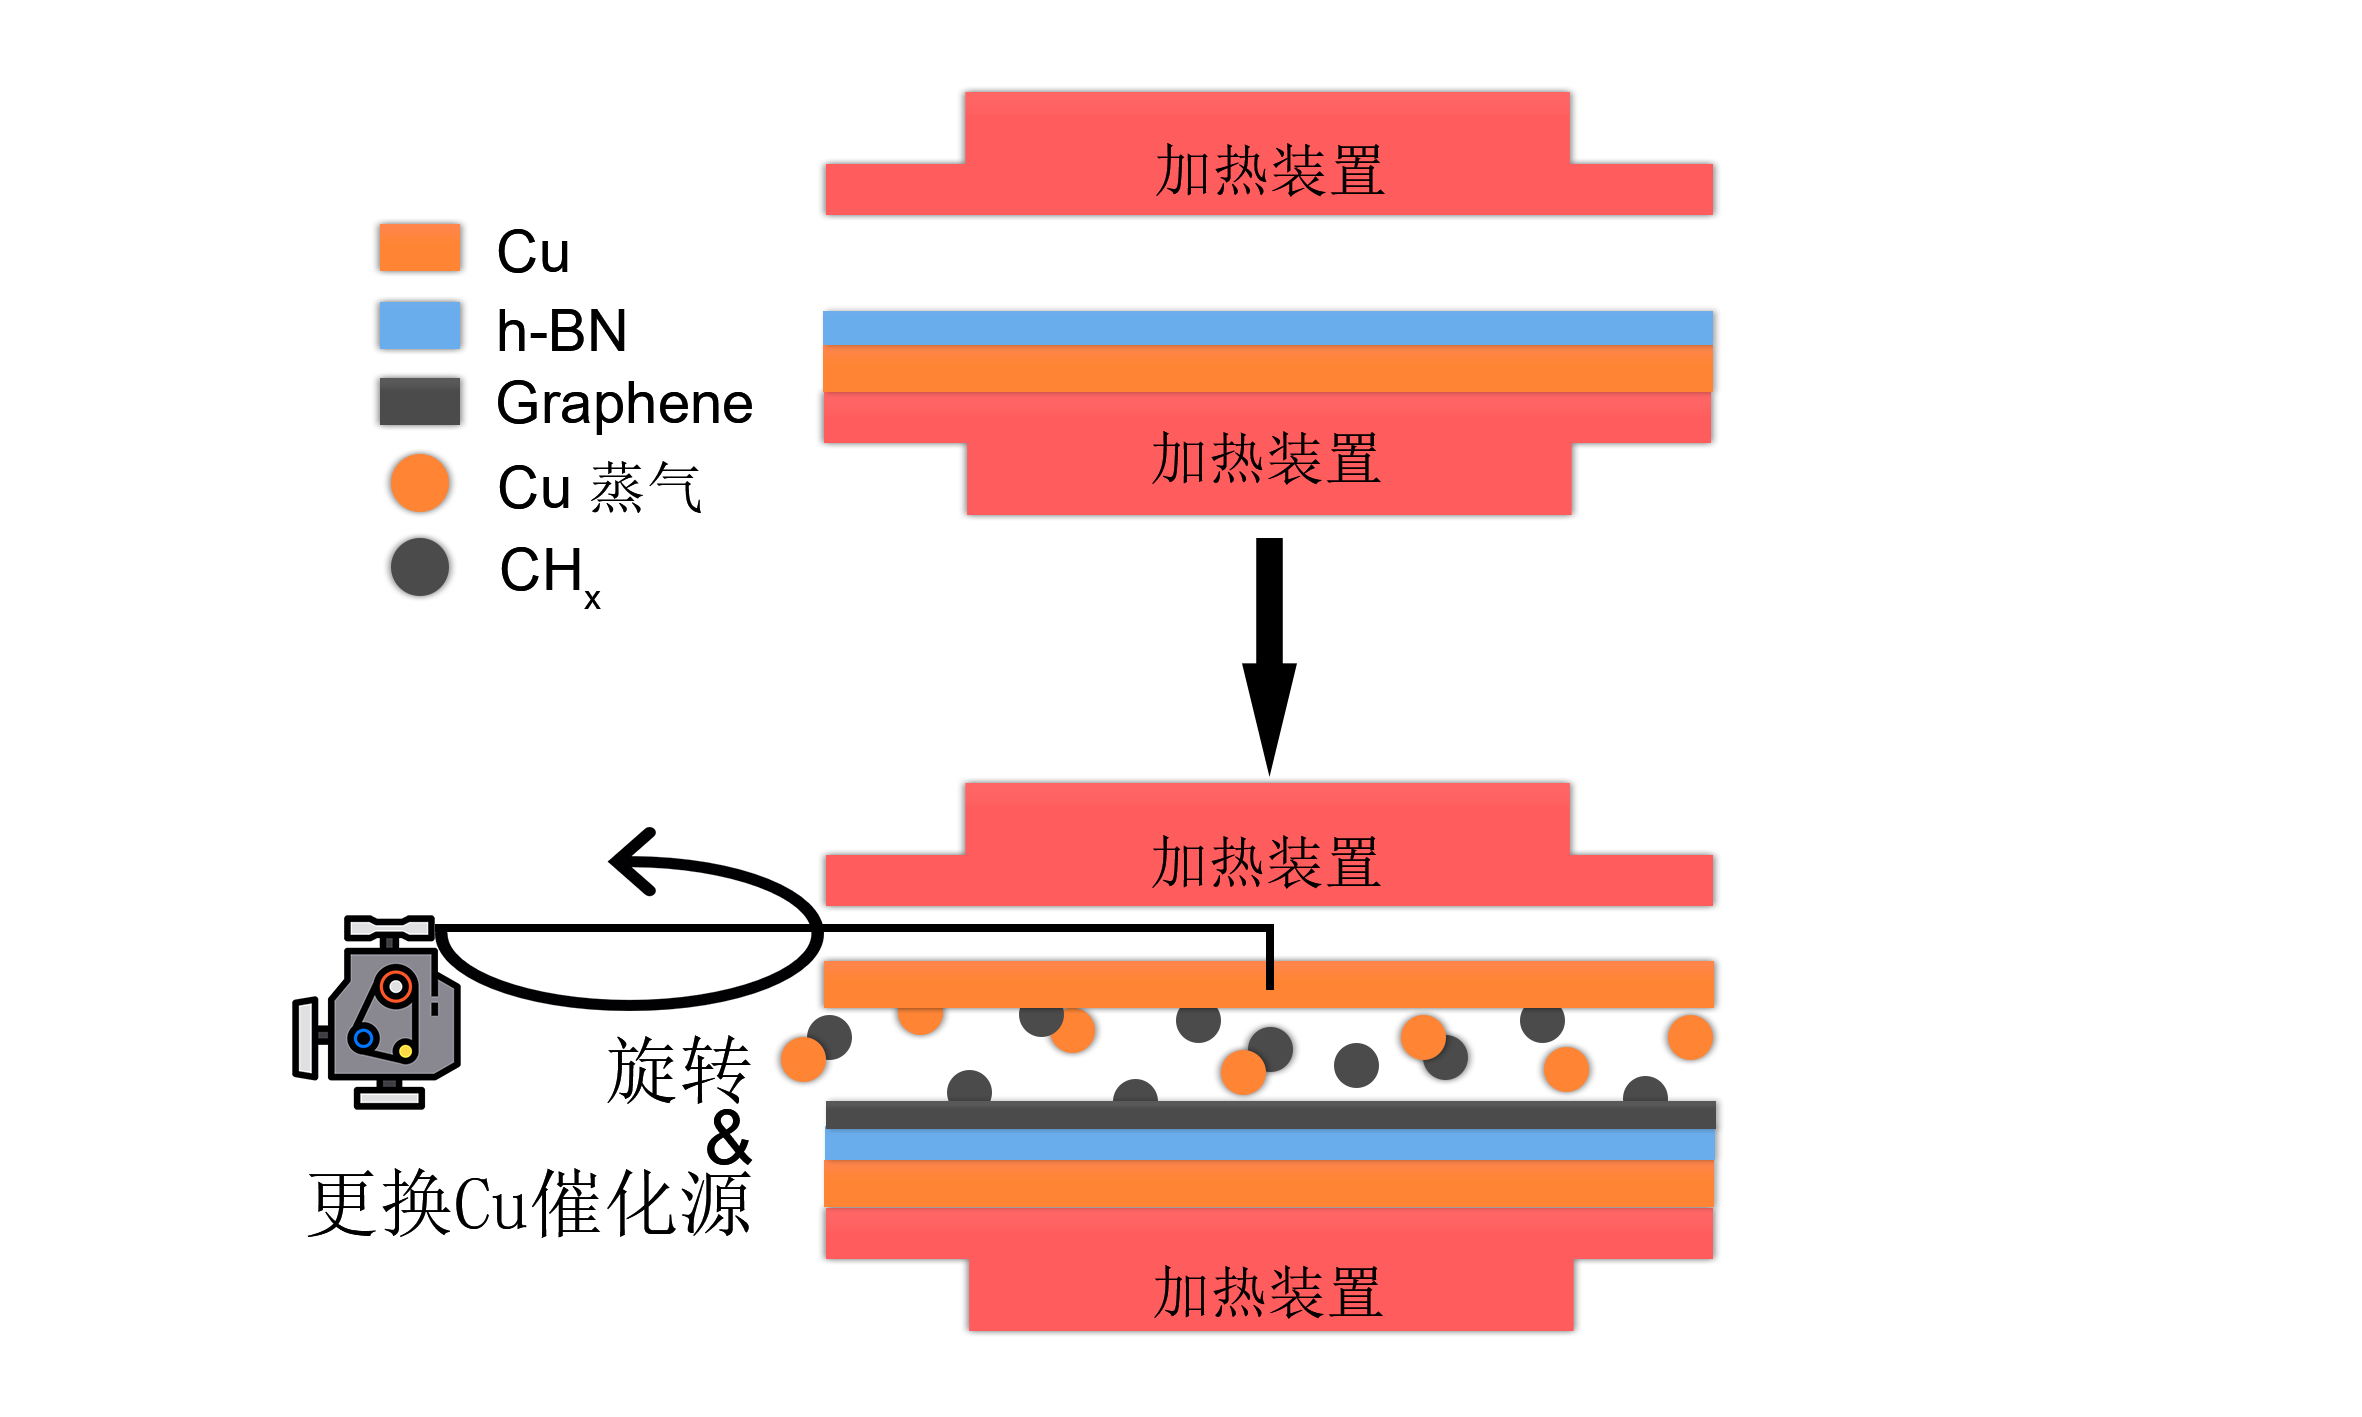
\includegraphics{pic/CG_diagram_routine.png}
            \label{fig:CG_diagram_routine}
        }
        \newline
        \subfloat[]{
            \includegraphics{pic/CG_diagram_growthSketch.png}
            \label{fig:CG_diagram_growthSketch}
        }
        \caption{利用\cemb{Cu}蒸气近邻催化效应在\cemb{h-BN}表面直接堆叠生长石墨烯。(a)生长装置示意图;(b)石墨烯/\cemb{h-BN}异质结生长过程示意图}
        \label{fig:CG_diagram_CVD}
    \end{figure}

    \subsection{近邻蒸发气态\cemb{Cu}催化剂的扩散}
    
    \begin{figure}[htb]
        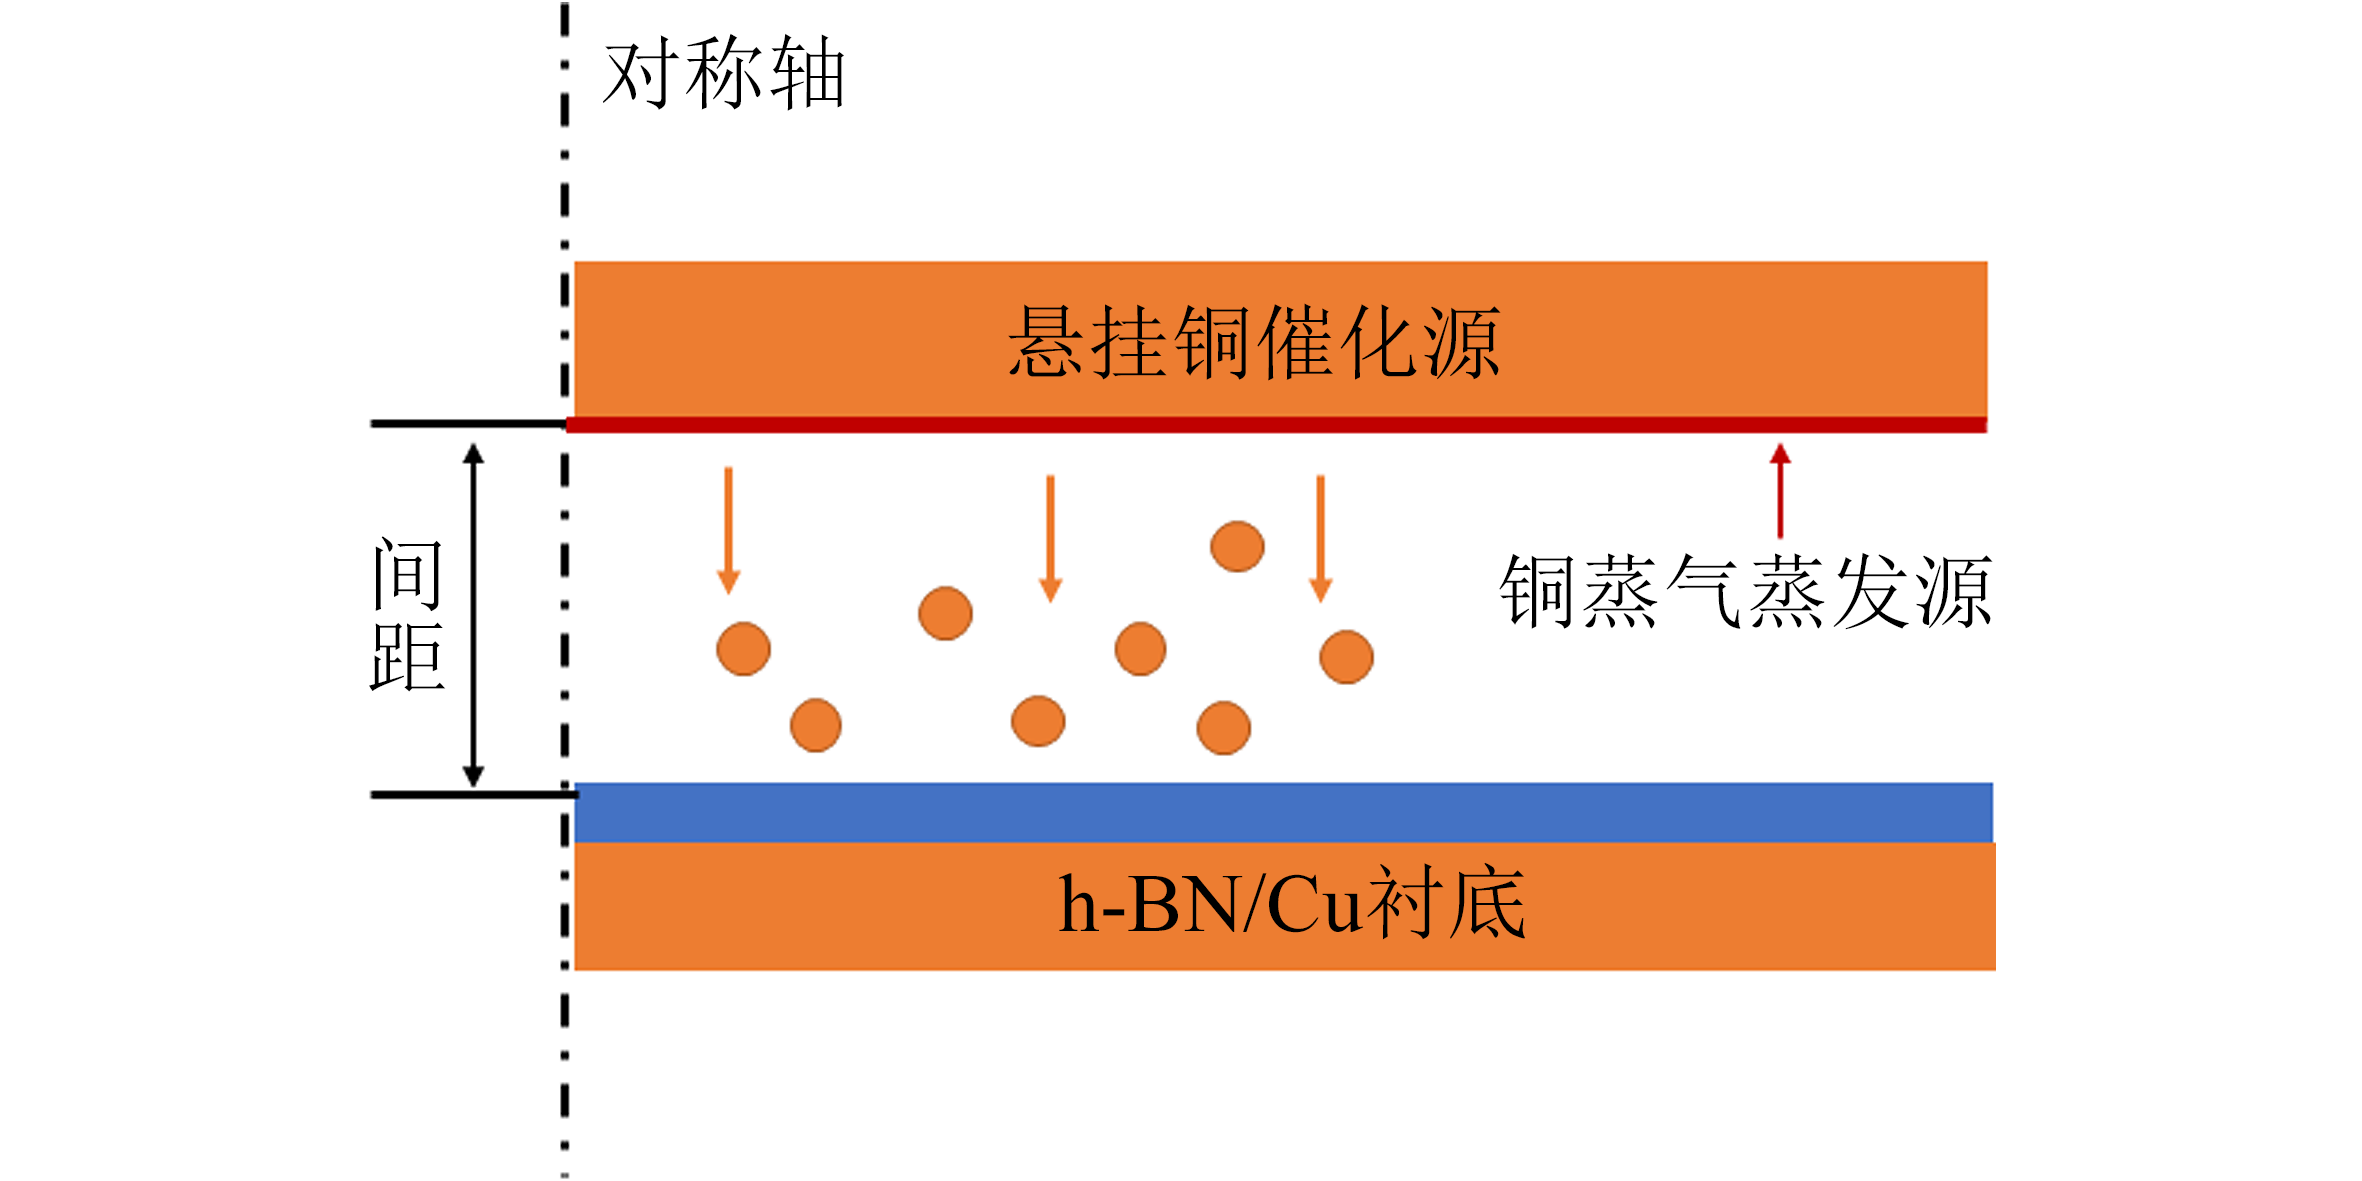
\includegraphics{pic/CG_diagram_FEM_structure.png}
        \caption{化学气相沉积腔体内\cemb{Cu}蒸气扩散模拟示意图。}
        \label{fig:CG_diagram_FEM_structure}
    \end{figure}

    \begin{figure}[htb]
        
    \end{figure}

    \subsection{气态\cemb{Cu}催化剂对甲烷裂解反应的催化性能}
    \subsection{\cemb{h-BN}表面石墨烯的生长演化机理}
\section{石墨烯/二硒化钒横向异质结的生长机理}
\section{总结}
    % LTeX: language=zh-CN
\chapter{总结与展望}
%//TODO 总结

    \thesisacknowledgement
\IfSubStr{\MYANONYMOUS}{Y}{
}{
    首先我要感谢我的导师牛晓滨教授。不知不觉间在牛老师的门下已经学习和研究超过了五年时间,牛老师
    %//TODO 致谢
}


    \thesisbibliography{reference}
    \thesisaccomplish{publications}
}{
    % LTeX: language=zh-CN
\begin{chineseabstract}
    具有优异的物理化学性质的二维材料及其异质结在电子,光电子等领域具有广阔的应用前景和不凡的研究价值。迄今为止,二维材料及其异质结在新型电子、光电子器件的研究中得到了大量的关注。大量隶属于不同材料体系的二维材料及其异质结被不同的实验手段制备合成。但是,由于二维材料复杂的生长过程和生长动力学机制,想要低成本、快速、形貌高可控地生长制备出大面积、高质量的二维材料及其异质结仍旧困难重重。首先是二维材料及其异质结生长过程中复杂的反应机理,衬底化学反应、气相化学反应,生长温度等各种参数的变化都会影响二维材料及其异质结的生长质量和形貌调控水平。其次是二维材料精细的电子结构进一步提高了对二维材料及其异质结生长质量和调控精确等级的要求。
    
    为了能够更好地理解二维材料及其异质结的生长过程,为二维材料及其异质结的高质量可控生长提供理论基础,本论文对多种二维材料和二维材料异质结进行了深入的机理研究,讨论了包括衬底、生长气氛在内的多种生长参数对于二维材料及其异质结生长过程和形貌演化的影响,建立了相应的生长模型。

    本论文首先从石墨烯出发,探究在化学气相沉积法中衬底对于单层石墨烯生长晶向的影响。研究发现衬底表面的台阶会改变石墨烯的成核机制。与平坦衬底上生长的石墨烯不同,在台阶边缘生长的石墨烯会自发的向优先生长方向进行结构演化,实现石墨烯在多晶铜衬底表面的多点自发定向生长。多点自发定向生长的石墨烯能够大幅减少石墨烯晶畴之间的晶界,实现大面积石墨烯单晶的快速生长。随后,本论文进一步探究了气相沉积法生长石墨烯过程中化学气氛对于多层石墨烯的生长作用。深入研究了气氛中的氧对于多层石墨烯的生长和蚀刻行为的非均一促进机制。通过对氧促生长、氧促蚀刻之间竞争关系的进一步探究,建立了氧通量调控的多层石墨烯生长、蚀刻模式切换模型,绘制了相应的生长模式切换相图。对于石墨烯生长机理的研究为石墨烯单层大面积单晶生长以及石墨烯多层调控提供了理论基础。

    接着,本论文将研究扩展到具有结构极性的非平面二维材料。相比于平面二维材料,非平面极性二维材料具有更复杂晶体结构和生长机理。通过对非平面二维材料\cemb{InSb(111)}在\cemb{Bi(001)}衬底表面进行系统的分析计算,本论文探究了双层\cemb{InSb}从原子吸附到非晶态单层生长再到双层\cemb{In}极性自极化的整个生长过程和极性演化规律,揭示了\cemb{Bi}衬底表面单原子层\cemb{InSb}的非晶态构型,探究了双层\cemb{InSb}由非晶态构型极化至\cemb{In}极性过程的结构演化过程并且绘制了双层\cemb{InSb}的生长极性演化相图。最后,通过将表面能和界面能解耦的方式,本论文深入探讨了这两种能量在单层\cemb{InSb}生长、双层\cemb{InSb}自极化过程中的对于原子形貌的作用和竞争机制。研究发现非晶态单层\cemb{InSb}来源于\cemb{Bi}衬底对\cemb{InSb}强烈的相互作用,而双层\cemb{InSb}的极化则归功于二层重构\cemb{InSb}表面能的大幅下降。对于双层\cemb{InSb(111)}生长机理和极性演化机制的研究有利于加深我们对低维III-V化合物半导体纳米结构生长过程的理解,帮助我们其生长过程和生长形貌进行更有效地控制。

    最后,本论文在二维材料生长机理研究的基础上对纵向堆叠的石墨烯/\cembNHS{h-BN}二维材料异质结和横向拼接的石墨烯/\cembNHS{VSe2}二维材料异质结的生长机理进行了探索。提出并证明了利用\cemb{Cu}蒸气在\cemb{h-BN}表面催化裂解\cemb{CH4},加速生长石墨烯/\cembNHS{h-BN}纵向二维异质结的方法及可行性。探究了石墨烯在\cemb{h-BN}表面的生长序列,给出了石墨烯早期生长阶段从线性团簇到环形团簇到六边形团簇的形貌演化过程。对石墨烯/\cembNHS{VSe2}横向二维异质结生长机理的研究发现石墨烯/\cembNHS{VSe2}横向异质结的生长需要高活性的\cemb{V}、\cemb{Se}自由基作为生长前驱体。同时考虑热力学和动力学的生长因素,本论文发现了单层\cemb{VSe2}在双层石墨烯台阶边缘的选择性生长机制。对于二维材料异质结生长机制的探究为石墨烯/\cembNHS{h-BN}纵向二维异质结的生长提供了快速高效且不引入额外杂质的生长方式;对石墨烯/\cembNHS{VSe2}横向二维异质结生长机理的研究给出了异质结生长的限制条件,\cemb{VSe2}的选择性生长为异质结的空间位置可控生长提供了新的思路。

    本论文对于二维材料及其异质结的生长机理的研究为更低成本、更高质量、形貌调控更精确的二维材料及其异质结的生长方式提供了丰富的理论基础和有效的理论模型,有利于进一步推进二维材料及其异质结的实用化水平。

    \chinesekeyword{生长机理,理论计算,二维材料,二维材料异质结}
\end{chineseabstract}
    % LTeX: language=en-US
\begin{englishabstract}
    Two-dimensional materials and its heterostructures with excellent physical and chemical properties have broad application prospects and extraordinary research value in the fields of electronics and optoelectronics.

    Various 2D materials and 2D material heterostructures have been synthesized by different synthesis methods. However, due to the complex growth process and growth  mechanism of 2D materials, it is still difficult to synthesis large-area, high-quality 2D materials and two-dimensional heterostructures in a low-cost, fast, and highly controllable way. The first obstruction is the complex reaction mechanism in the growth process of two-dimensional materials. Small changes in  parameters such as substrate chemical reaction, gas-phase chemical reaction, and growth temperature will heavily affect the growth quality and morphology of two-dimensional materials and two-dimensional heterostructures. Secondly, the fine electronic structure of two-dimensional materials further improves the requirements for the growth quality and control precision level of two-dimensional materials and two-dimensional heterostructures.

    This dissertation aim to make better understanding of the growth process and provide theoretical reference for high-quality and highly controllable growth method of two-dimensional materials and its heterostructures. In this dissertation, growth process and mechanism of two-dimensional materials and its heterostructures were carefully investigated. Substrate, growth atmosphere and other growth parameters were studied and discussed for their influence of the growth process and morphology evolution of two-dimensional materials and its heterostructures. The corresponding growth mechanisms and growth model was addressed.

    Starting from graphene, this paper explored the substrate factors on the growth of graphene in chemical vapor deposition(CVD). The steps on the substrate surface can alter the nucleation behavior of graphene domain in early growth stage. Different from the flat Cu substrate, the graphene grow beside the steps on Cu substrate tends to spontaneously evolve to the most preferred growth orientation, which make the multipoint orientated growth of graphene on the polycrystalline Cu substrate possible. The multipoint orientated growth of graphene can greatly reduce the grain boundaries between graphene domains and realize the rapid growth of large-area graphene single crystals.
    
    % Dissertation
    %//TODO english abstract need to be done
    
    \englishkeyword{Growth Mechanism, Theoretical Calculation, Two-dimensional Materials, Two-dimensional Heterostructures}
\end{englishabstract}
    \IfSubStr{\MYCAPFLAG}{-1-}{% LTeX: language=zh-CN
% TODO LIST
% 第一章 绪论
% 二维材料及其异质结
%%% 背景
%%%% 二维材料
%%%% 二维材料异质结
%%%% 实验现状
%%%% 理论现状
\chapter{绪\hspace{6pt}论}

\section{二维材料及其异质结概述}
\subsection{二维材料概述}
自从石墨烯被发现并且成功大规模制备以来\citing{RN801-2009},二维材料由于其独特的电子结构、极强的声光耦合、奇异的层间作用、多样化的性质调控手段,已经引起了大量研究者的关注。至今为止,已经有包括石墨烯在内的多种体系的二维材料被理论上预言并在成功的实验中制备,例如与石墨烯结构相似的六方氮化硼(Hexagonal boron nitride,h-BN),黑鳞(Black phosphorus,BP),二维过渡族金属硫族化合物(Transition metal dichalcogenides, TMDS)以及二维金属氧化物(Metal oxides),二维三五族半导体(III-V component semiconductors, III-Vs)等。这些二维材料来源于不同的材料体系,因此也具有各自截然不同的物理性质。%//TODO 引用

从材料性质的广度上看,多元化的二维材料赋予了二维材料器件更多,更自由的选择空间。以电子性质为例,不论是绝缘体还是半导体亦或是导体、半金属,都可以找到相对应的二维材料。
%//电子结构
在二维过渡金属硫化物中,以不同元素组成的二维金属硫化物材料虽然都具有相似的晶体结构,但其各自的电子性质确有很大的差异\citing{RN956-2015}。在二维过渡金属硫化物中,以六族元素硫,硒,碲和过渡金属铬,钼,钨组成的二维材料具有直接带隙,其禁带范围囊括0.5 eV至2.5 eV。而以其他六族元素和过渡金属组成的二维金属硫化物则表现出具有间接带隙的电子结构,且禁带范围扩展为0.9 eV至7.0 eV。如此宽泛的电子结构分布使得研究者可以仅仅使用二维过渡金属硫化物材料就可以组合出具有一型、二型和三型能带匹配的的半导体异质结,可用于制造包括发光二极管(一型能带匹配),单极、双极型电子器件(二型能带匹配),隧穿场效应管(三型能带匹配)等\citing{RN357-2016, RN958-2018}。
%//光电
多样化的的电子结构同样赋予了二维材料极宽的光响应频谱,其可以覆盖从紫外到太赫兹甚至微波的电磁波频段。当厚度逐渐减少至单原子层变为二维材料后,材料的电子性质可能会发生奇异的变化。例如在过渡族金属硫族化合物中,MoS$_2$, WS$_2$,WSe$_2$等材料的电子结构会发生变化,由块体状态下的间接带隙半导体变为二维状态下的直接带隙半导体\citing{RN984-2010,RN985-2013,RN986-2015}。电子结构的变化使得二维化的MoS$_2$的发光量子效率相比于块体状态提升了4个数量级\citing{RN984-2010}。尽管只有单层或者是几层原子的厚度,二维材料独特的电子结构使其能够与光产生奇异的相互作用。例如单层的二维二硫化钼材料可以通过激子共振的方式吸收大约10\%的对应共振频率的光线。此外,过渡族金属硫族化合物的二维化显著降低了库伦作用的介电屏蔽效应。二维过渡族金属硫化物中较强的库伦作用大幅提高了其中激子的结合能,进而提升了材料的光响应速率\citing{RN987-2014,RN988-2013}。以单层硫化钼(MoS$_2$)为例,通过理论计算预测的其激子结合能在0.5 eV到1 eV\citing{RN989-2012,RN990-2013},大大高于传统的准二维半导体量子阱\citing{RN991-1984,RN992-1981}。而对于石墨烯而言,其布里渊区内独特的狄拉克锥电子结构导致了石墨烯具有许多独特的光电性质。例如石墨烯具有约2.3\%的宽带吸收率,使其可以作为可饱和吸收器件、光子探测器以及调制器等光电器件的候选材料。同时,包括饱和吸收效应,高次谐波产生效应,合频产生效应,四波混频效应等非线性光学效应也在以石墨烯、过渡族金属硫族化合物等二维材料体系中被发现。尤其是对于过渡族金属硫族化合物体系,其面外方向的反演对称性可通过层状堆叠打破,产生在其他二维材料无法实现的偶数次谐波效应。%//FIXME 引用

%//催化
同样,二维材料独特的晶体结构和电子特性也引起了大量化学催化方面研究者的关注。得益于多样化并可精细调控的电子性质,利用二维材料制得的催化剂对那些对于低能级反应尤其有效。如氧气,一氧化碳,二氧化碳,甲烷,水等小分子之间的转化,这些反应对催化剂表面电子结构较为敏感,可以最大可能的利用二维材料表面电子结构精细可调的优势。二维材料平面化的晶体结构为活性催化基团提供了精细可调的锚定位点,催化位点的电子态可以被精细调控至相应的催化底物能级,实现整体催化活性的调控。利用这样的原理,使用石墨烯,过渡金属硫化物等二维材料作为承载面,将过渡族金属原子等活性催化单元直接嵌入二维材料的平面,可以制得新能优异的单原子催化剂\citing{RN1019-2019}。在2015年,研究者通过在石墨烯表面参杂Ni制备单原子催化剂用于酸性环境下的析氢反应,其催化性能远超镍基催化剂并且具有极高的循环稳定性\citing{RN1018-2015}。随后,通过系统的理论计算,研究者在氮参杂的石墨烯上筛选出V,Rh,Ir等金属原子作为单原子催化剂,可以显著提升析氢反应的催化性能\citing{RN1015-2020,RN1017-2019}。在2020年,有研究者报道使用ZIF8作为前驱体进行热熔解,可以获得高比表面积的Fe-N参杂石墨烯单原子催化剂,其催化性能与已经大规模商品化的Pt/C催化剂不相上下\citing{RN1016-2020}。出了石墨烯外,以过渡金属硫化物为代表的其他二维材料也作为单原子催化剂的潜在载体进入了研究者的视线。在2020年,通过使用H$_2$O$_2$对MoS$_2$进行化学腐蚀的方式,研究者在二维MoS$_2$表面获得了单S空位的催化剂,并且实现了对S空位分布的综合调控以及较强的析氢催化活性\citing{RN1020-2020}。同年,另一组研究者利用激光分子束外延的手段实现了二维CrS$_2$表面的单原子Mo参杂,CrS$_2$的表面环境极大地提升了Mo原子周围的电场水平,使得其析氢催化的性能在极大提升的同时仍然保持了较高的稳定性\citing{RN1021-2022}。
%//FIXME 引用

从材料性质的深度上看,二维材料同样拥有优异物理化学特性,具有非常高的应用潜力。在过去的十年中,二维材料所展现出的丰富的新物理激发了基础物理和技术应用方面的广泛研究。例如以石墨烯,二硫化钼($\rm{MoS_{2}}$) 以及黑鳞(BP)等为代表的二维半导体材料具有极高的载流子迁移率和相当优异的机械性能,非常适用于制造下一代低功耗高速电子器件和柔性器件。同样,以六方氮化硼,金属氟化物(如$\rm{CaF_{2}}$, $\rm{TiF_{2}}$)为代表二维绝缘体材料拥有惰性的上下表面,能够很好的与其他二维材料形成范德华界面。其作为电介质层能够极大程度地减少场效应管中沟道材料的缺陷态密度,尽可能地发挥先进沟道材料卓越的输运性能。二维材料不仅能够在现有成熟器件框架下利用其优异地物理化学性质进一步提升电子器件的性能,其独特的电子结构让研究者能够突破传统电子器件的限制,对电流以外的电子自由度进行操控。例如,石墨烯体系中超低的自旋-轨道耦合使其能够很好地保持在其上传输的自旋信息,是理想的自旋电流传输材料。而二维过渡金属硫化物体系中较强的自旋-轨道耦合性质使其能够有效地对自旋进行操控,是非常好地自旋编码材料。同时,二维材料独特的单层结构使得其电子中的能谷结构可以很容易地被附加的作用场调控,简并分裂的电子能谷作为额外的自由度可以看成赝自旋并用作信息处理的载体。
%这种利用电子的自旋特性,通过对电子的自旋自由度进行操作编码来进行信息处理的自旋电子器件,由于其可编程逻辑元件和非易失性信息存储器件等不同领域的应用而备受研究者的关注。随着微加工技术和大规模集成电路的发展,电子器件尺寸进一步缩小的需求与日俱增。
相比于传统电子器件中依赖电荷输运来进行信息处理的方式,通过操控电子自旋进行信息处理具有速度更快,能耗更低,集成读和稳定性更好的特点。这些特性使得具有自旋输运特性的体系在未来的数据存储,数据传输以及数据处理方面都有着极大的发展潜力[42]。%//FIXME 引用,语言

%//超导
二维材料提供了绝佳的电子结构调控平台,使得研究者能够更好的基于现有理论发现新的物理现象、制造新的器件。而二维材料奇异的电子结构同样为新物理理论的产生提供了土壤。在二维材料中,因为具有开放的双面表面,原则上所有原子都受到表面反应的影响。同时,电荷和声子输运被严格限制在每一层中,因此其具有不同于三维体材料的特殊物理性质。以石墨烯为例,电子与蜂窝状碳晶格的相互作用使电子表现为无质量费米子,从而产生了反常的室温量子霍尔效应和极高的载流子迁移率等新的物理现象。在2008年,研究者测量到了石墨烯中电子的局域态分布,证实在石墨烯量子点中电子和空穴的由于无序效应引入的积水潭(puddle)的存在形式,解释了石墨烯中零载流子密度和非零电导同时存在的现象\citing{RN998-2008}。%//TODO。
在2012年,研究者在单层$\rm{FeSe/SrTiO_{3}}$中发现了非经典的高温超导态,揭示了在二维材料中存在传统超导理论(BCS理论)难以解释的反常超导现象\citing{RN953-2012}。而且在$\rm{FeSe/SrTiO_{3}}$系统中,超导态仅在单层$\rm{FeSe}$的情况下被发现,并且随着$\rm{FeSe}$厚度的增长消失。更加印证了在二维材料中具有有别于块体材料的超导现象。相比于$\rm{FeSe/SrTiO_{3}}$这样复杂的系统,另一个非经典超导现象在简单的石墨烯体系中被研究者所熟知\citing{RN954-2018, RN955-2018}。在扭转双层石墨烯(Twisted bilayer graphene, TBG)中,载流子的填充水平可以简单地被双层石墨烯之间的扭转角度所调控,使其能够从莫特绝缘体转变为超导体。
%//TODO 多一些转角

%//量子计算
同时,以石墨烯为代表的多种二维材料是天然的二维电子气载体,因此在量子计算和量子晶体管方面的应用方面具有独特的优势。自2007年提出可以利用二维材料石墨烯实现自旋量子比特的理论方案\citing{RN997-2007}以来,二维材料用于量子晶体管方面的研究已有较多进展。在2008年,研究者首次在二维材料石墨烯上采用刻蚀方法实现了栅极调制的单量子点结构,成功地实现了量子晶体管\citing{RN996-2008}。2009年,研究者测量了磁场调控下石墨烯量子点的电子附加能谱(Addition Spectrum)。通过对附加能谱中电子-空穴交叉的研究,研究者得到了石墨烯量子点的线性色散和边缘限制的光谱随磁场的变化情况,为石墨烯量子点电子输运行为的磁场调控提供了理论基础\citing{RN999-2009}。在2010年,自旋态以及自旋过滤现象在石墨烯量子点中测得,研究者可以通过操控外加磁场的方式调控石墨烯量子点中的自选过滤行为\citing{RN1000-2010}。在2013年,研究者成功的在石墨烯量子点中测量了激发态能级弛豫时间,证明石墨烯量子点中能级弛豫时间和GaAs等材料基本一致,都在100纳秒量级\citing{RN1001-2013}。这些一系列的研究,使我们对石墨烯以及石墨烯量子点中的电子性质的理解更加深入,更多调控手段的引入使得以石墨烯、石墨烯量子点为基础的量子晶体管的研究得到进一步发展。在2010年,研究者在石墨烯上实现了栅极可控双量子点量子器件,研究者可以通过栅极调控量子点中的电荷数量,进而调控量子点间的电子耦合特性和激子输运特性\citing{RN1002-2010}。同年,研究者通过在石墨烯大小双量子点的方式,将大石墨烯量子点作为单电荷晶体管集成在小石墨烯量子点上,并成功测量了栅极可控的小石墨烯量子点上的电荷态\citing{RN1004-2010}。在2011年,研究者成果测量了利用单、双层石墨烯制备的平行耦合双量子点的输运性质\citing{RN1005-2011},并在2012年实现了多栅极可控的石墨烯双量子点中激发态能级的测量\citing{RN1006-2012}。同年,研究者通过在空气中使用电流烧蚀的方式制得石墨烯量子点,进一步拓宽了石墨烯量子点的大规模制备手段\citing{RN1003-2012}。其高达1.6 eV的载流子附加能(addition energy)为同时期的最高水平,可用于制备单量子晶体管。2015年,研究者探究出了石墨烯量子晶体管和超导微波腔的色散耦合方式,并实现了量子晶体管的微波场调控\citing{RN1007-2015},以及通过维波谐振器实现的两个石墨烯量子点的长程耦合\citing{RN1008-2015}。

这些尝试证明了在石墨烯上可以实现量子结构并进一步制成量子晶体管,但是由于石墨烯不是真正意义上的半导体,不具有直接带隙,因此在多场可调性和量子操作性上仍有一定局限。因此,近年来许多研究者开始探索以MoS$_2$为代表的二维过渡族金属硫族化物用于实现量子晶体管的可能性。
2015年,研究者利用纵向二维异质结作为测量平台,对MoS$_2$的输运性质进行了精确测量,获得了高达34000 cm$^2$V$^-2$s$^-1$的霍尔迁移率\citing{RN993-2015}。同年,研究者在二维WSe$_2$上的实现了门定义的单量子点结构,其隧穿势垒可由电场进行控制,而量子点的尺寸可以由相应门电极上的电压控制\citing{RN1011-2015}。相比于传统的GaAs/AlGaAs异质结,该工作进一步减小了二维过渡族金属硫化物上量子点结构的尺寸。在2016年,研究者在单层MoS$_2$上实现了单电子晶体管,并且用输运方法测量到了库伦阻塞效应\citing{RN994-2016}。2017年,研究者利用MoS$_2$和石墨烯组成的异质结实现了栅极可控的一维量子通道\citing{RN995-2017}。2017年,研究者成果测量了单层MoS$_2$在磁场中的量子输运现象及演化规律,观察到了单层MoS$_2$中量子化的电导并深入探究了MoS$_2$导带中的自选劈裂现象,并认为其可以用于制备新型二维量子自旋器件\citing{RN1009-2017}。同年,研究者在二维材料MoS2中制备了电学可调的门控双量子点结构,首次在二维材料中实现了从双量子点到单量子点的可控调节\citing{RN1014-2017}。2018年,研究者在二维MoS$_2$中实现了门控的单量子点结构,并利用量子输运方法测量到了单电子的电荷态和激子态\citing{RN1010-2018}。同时,由于二维拓朴层状材料的发现,研究者成功的在实验中观测到了二维WTe$_2$体系中由边界态传输的量子化电导,在100K地温度下,二维WTe$_2$表现出了内部绝缘,边缘导电的奇异量子态,为量子晶体管中量子态的调控提供了新的手段\citing{RN1022-2017}。
%利用二维拓扑体系中可用gate调控拓朴性的特点,在2D拓朴材料上实现Majorana费米子,在接下来设计复杂交换结构时仅仅需要利用半导体加工技术在材料上设计gate结构即可。

除了优异的材料性质之外,二维材料由于其平面化的结构特点,能够较好地与与现行集成电路使用的平面硅工艺兼容。以二维材料制成的二维纳米器件能够较为容易的在现有的芯片集成,可作为新一代纳米电子器件的候选材料。


\subsection{二维材料异质结概述}
电子器件的基本组成元件为异质结,通过对二维材料进行纵向堆叠或者平面组装而形成的二维材料异质结能够结合不同二维材料优异的物理特性,最大化的利用其性质多样化的特点\citing{RN370-2017, RN380-2012, RN369-2014, RN371-2014, RN357-2016, RN353-2017, RN385-2014, RN351-2014, RN316-2018, RN387-2012, RN368-2017}。 而二维材料较弱的层间作用和相似的平面结构为二维材料异质结稳定界面的形成提供了保证。得益于其优秀的性质,二维材料异质结近年来发展迅速。早在2010年, Dean等人通过将剥离的单层石墨烯转移到六方氮化硼上,制成了由两个单原子层的二维材料组成的异质结。在那之后,由于其独特的界面激子效应和优异的光伏相应特性,包括石墨烯/六方氮化硼,石墨烯/过渡金属硫化物,过渡金属硫化物/过渡金属硫化物在内的多种二维材料异质结引起了大量研究者的关注。迄今为止,已经有多种二维异质结通过实验合成\citing{RN961-2018, RN960-2018, RN351-2014}并用于制造场效应管\citing{RN386-2012, RN387-2012}、存储器件\citing{RN389-2013, RN388-2011}、光电器件\citing{RN390-2013}等。二维异质结使得功能更强大、特性更新颖的电子器件的出现成为了可能。

%//二维材料异质结
由于机械剥离和转移技术的成熟,将二维材料进行纵向堆叠而成的纵向异质结首先进入研究者的视线。2010年,研究者通过机械剥离的方式的将单层石墨烯转移到二维六方氮化硼上,形成了具有原子层级厚度的异质结\citing{RN959-2010}。从那时起,包括 graphene/h-BN,graphene/TMDs,TMDs/TMDs 在内的大量纵向二维异质结引起了研究者的广泛关注\citing{RN309-2015, RN384-2015, RN319-2017, RN383-2012, RN368-2017},包括界面激子效应,谷电子效应和光伏响应等优异的物理性质也被逐一从二维材料异质结之中发掘出来。例如,自2015年起,已有研究者通过理论计算发现,可以将单层SnSe$_2$与单层MoS$_2$进行堆叠形成一型能带匹配的半导体异质结。其具有的超快电子-空穴复合效应使其非常适合用于制造发光二极管等光电器件\citing{RN966-2019,RN978-2017,RN979-2015}。对于二型能带匹配,由于导带底和价带顶分属于不同材料中,因此二型能带匹配可以用于电子和空穴的高效分离。若是将二维材料进行堆叠形成具有二型能带匹配的异质结,那么二维材料之间的范德华区域将对电子和空穴的相互作用产生屏蔽效应,可以对电子和空穴进行有效分离,导致其激子寿命长于普通材料\citing{RN969-2015,RN970-2015}。自2018年起,已有研究者分别从实验和理论计算的角度证实,在二维过渡族金属硫族化合物异质结,二维III-VI族化合物异质结等二维异质结体系中均可观测到持续时间非常长的电子-空穴分离态\citing{RN976-2020,RN975-2019,RN972-2017,RN977-2018}。而在二维Janus材料和二维钼硫硒化合物(MoSSe)组成的具有二型能带匹配的双原子层异质结中,在2019年已有理论计算预测其具有长达16.5 ns的激子寿命\citing{RN971-2019}。对于具有三型能带匹配的异质结,其破缺的能带结构允许载流子在不同材料的能带之间隧穿,使其能够作为隧道场效应管的基础结构。例如,黑磷/硫化锌(Phosphorene/SnS$_2$),黑磷/硒化锌(Phosphorene/SnSe$_2$),硒化钨/硒化锌(WSe$_2$/SnSe$_2$)等材料可以组成具有三型能带匹配的异质结,已经有工作通过理论计算预测可以在这类二维异质结中观察到载流子的带间输运现象,是实现二维隧道场效应管的候选材料\citing{RN981-2018,RN982-2016,RN983-2017}。同时,由于三型能带匹配中电子和空穴的传输速度远高于二型能带匹配,大量的电子和空穴可以被迅速得分离到一直接种不同的材料上,使异质结内部产生一个较强的内建电场,并且显示出类似于半金属的特性。这样的特点使得具有三型能带匹配的异质结非常适合用于制造下一代新型热光伏太阳能电池\citing{RN980-2019}。
不仅如此,二维材料之间的能带匹配还能够通过外加电场等方式进行改变。例如,可以在单层硒化锌(SnSe$_2$)与单层硫化钼(MoS$_2$)形成的异质结中附加外加电场,使其从原来的一型能带匹配变为二型能带匹配\citing{RN966-2019}。在单层硫化锗(GeS)和砷烯(Arsenene)形成的异质结体系中,外加正电场可以其保持原有的二型能带匹配,而外加负电场可以使其转变为一型能带匹配\citing{RN967-2019}。而在磷/硫化锌(Phosphorene/SnS$_2$)形成的具有三型能带匹配的异质结中,外加负电场可以实现一型,二型,三型的能带匹配转变\citing{RN981-2018}。除了外加电场外,最新的研究发现可以通过施加应变应力的方式,将单层硼磷化合物(Boron phosphide)和单层MoSSe形成的的一型能带匹配转变为二型能带匹配\citing{RN968-2021}。

作为二维异质结的组成材料,引起研究者关注的不仅仅是那些具有半导体特性的二维材料。作为二维材料中的绝缘体,六方氮化硼在具有较大的带隙的同时也保有二维材料高质量面内结构的特点。趋近完美的二维晶体结构使得六方氮化硼在禁带内具有极低的缺陷态密度以及较高的击穿电压,使其能够在隧穿器件中作为非常好的势垒材料。同时,利用六方氮化硼高耐压的特性,将石墨烯和六方氮化硼进行堆叠,能够制成具有超薄介电层的电容器。超薄的介电层能够将小至单位电荷的变化情况传导到电极之中,使之成为量子电容器。量子电容器可用于测量量子输运体系中极其微小的电荷转移情况。运用类似的思路,将石墨烯、过渡金属硫化物以及黑磷等材料纵向堆叠成类三明治结构所制得的量子电容器也被大量研究者所关注。而最早发现的二维材料,石墨烯,其独特的电子结构使得可以通过引入外置栅极的方式对费米能级和态密度的位置进行调控,以此来操纵穿过势垒的隧穿电流的大小,适合用作隧穿器件中的源极和漏极材料。

与传统材料界面处的共价键相反,纵向二维材料异质结构中各层之间相对较弱的范德华力极大地放宽了晶格匹配和化合价的要求,最终实现了更宽的异质结构相空间。尽管很弱,但范德华相互作用仍然主导了跨界面的各种类型的耦合。例如,电荷在界面处重新分布以平衡化学势,这会影响诸如电荷屏蔽、能带弯曲和载流子耗尽等现象。尽管传统的三维异质结构和二维范德华结构均发生界面电荷转移,但二者存在显著差异。首先,范德华界面处较小的电子交叠将电荷层间转移的过程限制为相对低效的隧穿和跳跃。其次,由于范德华界面处介电屏蔽的减少而导致激子结合能的增加,消除了传统异质结中决定电荷转移过程的能带偏移。这些因素都导致在传统异质结的理论框架下,二维材料范德华异质结中不同材料直接的电荷转移是缓慢的。但是,最近的研究发现了在部分二维材料组成的范德华异质结构中,存在超快的电荷转移过程,包括MoS$_2$/WS$_2$,MoS$_2$/石墨烯,WS$_2$/石墨烯量子点和MoS$_2$/有机分子异质结构等\citing{RN523-2017, RN308-2014, RN520-2016}。%//FIXME 检查一下这几个例子
在二维超导体中,界面耦合也会强烈影响超导临界温度。例如,FeSe是研究最多的二维超导体之一,其体超导临界温度(Tc)约为≈8K。然而,通过在SrTiO3上生长单层FeSe,由于界面增强的电子-声子耦合,Tc显着提高到≈100K\citing{RN747-2014, RN746-2013, RN748-2018}。
除电子耦合外,自旋自由度还引入了界面磁耦合。自旋之间的交换相互作用决定了相邻电子之间的自旋排列方式,平行或反平行,对应于铁磁和反铁磁排序。对于铁磁层和反铁磁层形成的界面,在外部磁场为零的情况下下,界面处的排序类型由交换相互作用决定。通过施加外部磁场,反铁磁性层的磁化方向可以翻转到与外部磁场平行对其。这是因为即使交换相互作用使得反铁磁性层的界面能增加,但是外部磁场平行对齐的电子自旋仍然可以使总能量下降。通过交换相互作用和超快速电荷转移,当单层WSe2与CrI3集成在垂直异质结构中时,可以观察到其山谷极化得到了明显改善\citing{RN751-2018, RN752-2019}。//FIXME 修改

横向向二维异质结独特的结构使之具有许多出色的性能,在应用方面具有广阔的
前景。它们的电子特性也得到了广泛研究[29,38]。利用 MoS2-NbS2 横向异质结中的交错禁
带和弱耦合状态产生的传输间隙,可以制造出开关电流比为 106~107,漏电流约为 108
uA 的场效应晶体管[25];利用其纳米尺寸和多组分光学性质,横向 TMD 异质结可以用作单分子探测以及制造具有可调光响应的纳米器件[39];基于 WSe2-WS2 横向异质结的 p-n 结二极管和光电二极管,表现出了良好的整流特性并能产生较大的光电流[40];这些独特的优异性能使得横向二位异质结为制造更高性能互补逻辑电路、高频器件、及光电探测器等电子、光电子器件带来了新的可能。同时,由于横向二维异质结中普遍存在的自旋过滤效应,进一步推动了自旋电子学的发展。例如 ZGNR/g-C3N4 异质结和 h-BN/zigzag graphene 构建的异质结,都有着极高的自旋过滤效率[41]。组成横向异质结的两种材料之间的界线,其进一步降低的维数还可以带来更多的激发态物理性质 [29] 。

\section{二维材料及其异质结的生长制备和机理研究}
二维材料以其优异的电学、光学、化学、机械特性获得了大量研究者的关注。这些新颖的特性同时也为二维材料及其异质结带来了巨大的应用潜力和极高的理论研究价值。为了最大程度的研究了利用二维材料的诸多优异特性,研究者们一直在致力于研究二维材料及其异质结的高质量,高可控,大规模,低成本的合成方法。一般认为,二维材料及其异质结的合成方法可以分为两类,分别是自顶向下(top-down)合成方法和自底向上(bottom-up)合成方法。

自顶向下合成方法是最先运用于制备二维材料及其异质结的方式。在2004年,世界上第一种二维材料,石墨烯就是通过用胶带进行机械剥离的方式,从高定向裂解石墨块体中剥离下来\citing{RN1023-2004}。机械剥离可以在保留层内的共价键的同时,减弱块体材料中层间的范德瓦尔斯作用,使得单层状态的二维材料可以从相应的块体材料中分离。自2004年第一篇石墨烯被通过机械剥离的方法制备以来,机械剥离的方式在制备二维材料及二维异质结方面已经获得了广泛的应用\citing{RN1025-2021,RN1024-2016}。通常来说,机械剥离的方式能够制备具有极高质量的二维材料,并且可以精确的控制二维材料的层数,堆叠方式、晶向方向,旋转角度等参数,非常适合用作小规模的基础研究。虽然机械剥离是最早应用于制备二维材料的方法,但受限于较低生产效率和高昂的合成成本,剥离的方式很难应用于大规模的二维材料的生产制备。同时,机械剥离法在二维材料及其异质结的制备范围上也有限制,只能制备那些具有块体异构体和层与层之间作用力较小的二维材料。为此,研究者尝试了更多成本更低,制备效率更高的剥离方式代替原本手工剥离的方法,例如化学氧化-还原法、电化学剥离法以及液相剥离法等。这些方法使用化学插层或者液相超声的方式在溶液中产生大量悬浮的单层或者少层二维材料薄片,以此来大批量地制备所需的二维材料。但通常使用化学或者超声处理对块体材料进行分层剥离的方式很难精确地控制二维材料的层数分布,同时制备的二维材料往往会因为强烈的化学作用和超声震荡引入大量的杂质和缺陷,大幅度降低制备质量。虽然这些能够进行二维材料大规模制备的剥离方式很难在那些需要精确观测电子、声子、光子作用的基础研究中施展拳脚,但已有许多研究者将其应用到了催化领域的二维材料制备之中,并取得了较好的进展\citing{RN1026-2016}。

为了克服自顶向下合成方法的缺陷,研究者探索了通过自底向上的方式合成二维材料及其异质结。不同于需要相应块体材料的自顶向下的制备方式,二维材料及二维异质结自底向上的合成方法使用含有相应原子的前驱体,在衬底或者溶液中直接生长二维材料及二维材料异质结。使用自底向上合成的思路,已有包括物理气相沉积法(PVD)、化学气相沉积法(CVD)、原子层外延法(ALE)等方法被用于合成二维材料及二维材料异质结\citing{RN1029-2021}。虽然以化学气相沉积法为代表的自底向上的方式合成的二维材料以及二维异质结兼具高质量和可大规模生产的特点,但相对于机械剥离和化学剥离等自顶向下的合成方法,自底向上的合成方法通常需要如高真空、高温等更为严苛的合成环境,更加复杂的处理步骤。也因如此,二维材料及二维异质结的质量对自底向上合成方法的生长参数非常敏感,实验人员需要通过精确的参数调控,设计复杂的反应过程才能生长出理想的高质量大规模的二维材料及二维异质结\citing{RN1028-2019,RN1027-2018}。物理气相沉积法使用加热、离子撞击等方式使目标原子从靶材中脱离。脱离的气态原子在高真空的条件下附着在衬底上生在二维材料或者二维异质结。针对二维材料及二维异质结的合成,常用的物理气相沉积法包括溅射法,分子束外延法(MBE),激光脉冲沉积法(PLD)等。其中,分子束外延法可以对生长的二维材料及二维异质结的层数、表面结构以及化学计量数等形貌参数加以最高精度的控制。也正因如此,为了得到更好的生长质量,分子束外延的生长速率通常较低。


%参考用
%PVD使用加热的原子源在基板12上可控地沉积材料。对于合成元素2D材料(SE2DM)的生长,PVD通常需要超高真空(UHV)条件和校准良好的高纯度原子源。在超高压条件下制备的样品可以通过表面敏感技术进行现场研究,以保持材料的原始状态。CVD利用气体、液体或固体前体在受控气氛下的分解或反应来生长2D材料172173。对于CVD,催化活性底物通常是最有效的,并且可以在大气压到UHV的压力范围内进行合成。生长机制因基板而异:前体不溶性低的基板可能催化原子薄膜的自限生长,而其他基板则溶解大量前体,冷却后分离到表面。表面分解或分离利用生长衬底上的固态前体。当衬底被加热到足以激活升华或扩散过程时,生长发生,产生富含前体元素的表面层,然后冷凝为2D相。衬底选择仅限于包含前体元素的衬底,例如在SiC174上合成外延石墨烯。此外,可以从前体衬底上的非均匀薄膜(10–100nm厚度)开始,其加热有助于基于扩散的分离过程85175。

%参考用
%物理气相沉积包括多种技术,如分子束外延(MBE)、溅射和脉冲激光沉积(PLD)。对于2D材料的合成,MBE提供了对层厚度和化学计量的最高级别的控制。特别是,作为研究超导电性平台的复杂氧化物材料,只有通过氧化物分子束外延和PLD才能可靠地生长。生长过程中,元素源材料在超高压下从Knudsen电池(低温)或电子束蒸发器(高温)蒸发(图2g)。为了促进外延生长,生长速率通常较低。虽然MBE主要用于生长2D化合物,如NbSe2[132](图2h),但元素2D材料也已得到证明。[11,12,24–28,30,31]多层交替材料的连续生长能力对于创建二维异质结构和超晶格特别有用。[81]在PLD过程中,使用强激光烧蚀沉积靶材料,而不是使用热蒸发器。最近,这项技术已被用于生产许多二维材料,包括石墨烯、[133]hBN、[134]MoS2、[135]InSe、[136]和BP。[137]PLD的优势在于其高沉积速率和目标材料化学计量比的直接转移。然而,一个常见的问题是厚度没有得到很好的控制,由此产生的薄膜是高度多晶甚至非晶的。[137]最近的一篇综述全面总结了PLD在生长2D材料中的应用。[138]

%参考用
%https://sci-hub.se/10.1002/adma.201801586
%石墨烯层的合成已经投入了大量的精力,到目前为止,已经成功开发了几种石墨烯合成方法,例如石墨的机械剥离[1,19,20],液相剥离[21,22],氧化石墨烯(GO)的还原[23,24],单晶SiC晶片在高温下的超高真空升华[25,26],表面偏析[27,28],以及化学气相沉积(CVD)生长[29–31]。机械剥离法可以提供最高质量的石墨烯薄片,但由于难以控制薄片的层数和尺寸,因此不适合大规模生产。SiC基升华需要非常苛刻的合成条件,包括超高真空和1650K以上的高温。液相剥离和GO衍生不能制备高电子质量的石墨烯薄膜。化学气相沉积法(CVD)是合成石墨烯薄膜的主要方法,因为它同时满足大规模和相对高质量的要求。不同的金属衬底,包括Ni[27,28,30,32-34]、Cu[12,29,31,35-37]、Ru[38-40]、Ir[40-44]、Co[45,46]、Fe[47]、Au[48]、Rh[49]、Pt[50,51]及其合金[52,53],已被用于石墨烯薄膜的CVD合成。石墨烯在选择性绝缘衬底上无需转移直接生长,有望集成到硅基技术中。石墨烯层可以直接生长在绝缘衬底上,例如SiC[25,54]、蓝宝石[55]、SiO2[56,57]和h-BN[58,59]。基于密度泛函理论(DFT)和半经验紧束缚(TB)方法的计算表明,催化剂对碳原子在表面和亚表面的吸附、碳团簇的形成有影响,以及小薄片的稳定性,这些薄片是后续生长的前兆[39,60,61]。各种碳氢化合物原料已成功用作碳源,从甲烷[12,29,62]和乙烯[37]等气体,苯[63]等液体,到聚甲基丙烯酸甲酯(PMMA)[36]和无定形碳薄膜[64,65]等固体。原则上,任何含碳材料,包括食物、昆虫,甚至废物,都可以用来合成不同质量的石墨烯薄膜[66]。石墨烯生产中最常用的碳原料和衬底组合是CH4和Cu[67],因为很容易获得单层石墨烯(SLG)。这种组合已与卷对卷技术一起用于生产尺寸达30英寸的石墨烯薄片[12]。然而,铜上整个石墨烯片的均匀性仍有待改善。考虑到晶格匹配外延生长,Ni(111)衬底是生长高质量石墨烯薄膜的最佳平台,通过控制碳原子和Ni表面实现了广泛的SLG[27]。这表明CVD生长在高质量石墨烯薄膜的大规模生产中具有巨大潜力。

%参考用
%https://sci-hub.se/10.1002/adma.201801586
%由于自上而下的剥离倾向于产生相对较小的薄片,因此在需要大面积薄膜的应用中采用直接生长方法。在2D材料方面,CVD首次被用于在环境[15]和超高压条件下在金属衬底上制备石墨烯。[114]后来的发展使人们能够合成毫米大小、[115]厘米大小、[116117]甚至分米大小[118]的单晶石墨烯畴。同样,CVD是制备化学计量比、层数、畴大小和GBs可控的TMDC的最常用方法之一。如图2e所示,挥发性前体(如MoO3和S)共蒸发,然后反应,在目标基质表面形成所需的沉积物(如MoS2)。图2f显示了CVD生长的单层MoS2的示例。[54]最近的一篇综述文章总结了TMDC的典型CVD前体和生长条件。[119]此外,已经证明了CVD方法的几种变体。例如,石墨烯的等离子体增强CVD允许使用较低的衬底温度和生长时间,从而将金属衬底的污染降至最低。[120]此外,TMDC的金属-有机化学气相沉积(MOCVD)改善了大面积的生长均匀性[121122],而芳香分子辅助化学气相沉积促进了低温下大畴的生长[123],并有助于将不同的2D材料横向和纵向缝合成异质结构。[124]



\subsection{非极性二维材料}
%//TODO 石墨烯生长
%//TODO CVD
%//TODO 自限制生长

%%非极性二维材料
\subsection{极性二维材料}
%%极性二维材料
%%III-V半导体生长
\subsection{生长工艺及机理模型}
%//TODO https://sci-hub.se/10.1038/s41570-016-0014

%%纵向二维异质结
%%横向二维异质结
\subsection{纵向堆叠二维材料异质结}
对于纵向二维异质结,除了机械剥离法外,在已经制备的二维异质结中,现有的制备方法有图形再生长
(patterned regrowth)[45]、刻蚀再生长(etching regrowth)[46]、化学转化法(chemical 
conversion methods)[47]、一步法化学气相沉积(一步法, one-step CVD methods) [48,49]
和两步法化学气相沉积(两步法, two-step CVD method) [43,50]等。

%参考
%由于机械转移技术的现有局限性,开发一种直接在h-BN衬底上生长石墨烯的无转移技术非常重要。在早期的尝试中,Ding等人[52]首次报道了在粉末h-BN薄片上直接CVD生长少量层状石墨烯,然而,粉末h-BN薄片的粗糙表面和不规则形状导致生长石墨烯的质量差。后来,Son等人[53]和Tang等人[54]分别证明,可以通过常压CVD(APCVD)或低压CVD(LPCVD)工艺在机械剥离的h-BN表面上生长扁平石墨烯焊盘。这些石墨烯焊盘具有相对规则的圆形,但典型尺寸非常小,直径仅为100~200 nm。通过控制接近平衡CVD过程的小碳流,石墨烯畴的最大尺寸可以达到约11μm[55]。值得注意的是,由于h-BN的催化活性比过渡金属基底弱得多,石墨烯在剥落的h-BN上的生长速度非常慢,通常需要几个小时或几天才能完成制造。在h-BN上进一步精确定向生长石墨烯非常重要,这使得可以以可控的方式研究异质结构的性质和器件。2013年,Yang等人[56]利用远程等离子体增强CVD技术成功地在剥落的hBN上外延生长了石墨烯单晶(图2(a))。在生长过程中,甲烷分子通过远程等离子体源分解成各种反应性自由基,因此无需催化剂。AFM图像显示,所有石墨烯畴显示出相同的取向(图2(b)),表明石墨烯在h-BN上的生长遵循范德华外延模式。此外,由于石墨烯和h-BN之间的晶格失配较小,在Gr/h-BN异质结构上观察到了周期为15±1nm的三角云纹二维超晶格。Tang等人[57,58]也展示了类似的工作,他们进一步发现,作为气体催化剂的硅烷和锗烷可以显著提高h-BN上石墨烯的生长速率,比没有催化剂的石墨烯的生长速率高近两个数量级(图2(c,d))。因此,在h-BN上生长的石墨烯的最大磁畴尺寸可以在20分钟内达到20μm。理论计算表明,当加入催化剂时,石墨烯边缘碳物种掺入的阈值势垒大大降低,这是导致生长速率增加的原因。此外,气体催化剂的引入还有效地提高了h-BN上精确排列的畴的百分比,从约50%提高到93.1%或92%,为将来制造单晶Gr/h-BN晶片带来了希望


\subsection{横向堆叠二维材料异质结}

\subsection{生长工艺及机理模型}

%参考
%对于横向二维异质结,最为常用的合成方法是 CVD 法。横向的石墨烯和 hBN 异质结,最先在 2010 年被 Feng Liu, Pulickel M. Ajayan 等人采用一步法合成出来。这个单层结构的异质结在空间上是随机分布的,并且其带隙不同于纯石墨烯和 hBN[51]。在 2012 年,复合石墨烯和六方氮化硼薄层通过两步法合成[52],但是其形状和边缘难以控制。A. T. Charlie Johnson 等人采用了常压 CVD 法合成了有平直界面,且六方氮化硼沿着石墨烯晶体取向生长的二维异质结,其界面的清晰程度可以通过控制生长条件进行调控[53]。An-Ping Li,Gong Gu 等人采用两步法合成了石墨烯和六方氮化硼的异质结,通过对于第一步中合成的石墨烯层边缘的进行氢原子刻蚀,实现了 zigzag 形态的界面[54]。随着更多二维材料的涌现,过渡金属硫化物,特别是 MoS2 和 WSe2 受到了广泛关注。2014 年,Xiangfeng, Duan 等人通过横向外延的方式,用一步法制备了具有渐变无隙界面的WS2/WSe2 和 MoS2/MoSe2 异质结并且得到了很好的电子和光电特性[55]。Wu Zhou 和Pulickel M. Ajayan 等人采用一步法同时合成了横向和纵向异质结[3]。除了 CVD 方法外,MoSe2/MoS2 异质结也通过电子束光刻的方式合成[56]。由于一步合成的方法基于材料的自组装,我们很难控制二维异质结的形状和尺寸。同时对于 WX2 体系,因为金属和硫族元素同时发生了变化,一步法很难生长如同 WSe2-MoS2这样的异质结结,两步法的提出克服了这些困难。2015 年,有原子级的清晰界面的WSe2/MoS2 异质结通过两步外延生长方法成功合成[57]。 同时,Gong 等人设计了一个两步生成纵向和横向 WSe2/MoSe2 异质结的方法,能产生 169um 的异质结,且交叉污染相比之前的一步法要小很多。Cai 等人设计了一种新颖的采用离子交换方式的两步生长方法。采用这种方法,MoS2/ WSe2 异质结尺寸能长到 100um[58]。厚度调制的二维异质结也能采用 CVD 方法进行制备。Zhang 等人,制备了单层和双层阶梯状的异质结[59]。He 等人采用了 CVD 方法得到了了不同层数的 MoSe2 结。这对于层数控制的大尺寸异质结生长具有参考价值[60]。同时,图案化再生长和化学转化法也被用于合成二维异质结。在 2012 年,Mark P 等人使用了两步法合成了具有空间调制效应的六方氮化硼/石墨烯的异质结。他们先用 CVD 方法合成了石墨烯层,然后将石墨烯刻蚀形成特定图案,然后实现了 h-BN 层的空间选择性的生长[45]。Liu 等人,采用了两步 CVD 法合成了一个具有可控形状、清晰界面、大尺寸的六方氮化硼/石墨烯的异质结[61]。同时,MoSe2/MoS2 异质结也可以通过电子束光刻的方式合成。这种方法能够提供清晰界面,并且能够对图案和生长过程进行控制[56]。二维异质结也能使用物理气相转移,机械方法或者光刻等方法进行制备。Huang 等人采用气-固生长方法合成了一个无缝的高质量的横向 MoSe2–WSe2 异质结。并具有很好的光致发光特性[48]。在这些生长方法里,图形再生长法在制备上显得较为繁琐;刻蚀再生长、化学转化法则是利用化学反应对第一层单层二维材料薄膜进行刻蚀再生长或者直接转化,由于化学反应的复杂性,使得我们不能很好对二维异质结的生长进行较为精细的控制。而一步法虽然简单易操作,但是目前使用该方法制备出的二维材料异质结都在几十微米范围以内[3,63] ,并且使用一步法制备的二维异质结在两种二维材料交接处容易产生交叉污染或形成合金相,较难得到清晰的界面 [3,50] 。

%参考
%https://sci-hub.se/10.1088/1361-6633/aa9bbf
%石墨烯层的合成已经投入了大量的精力,到目前为止,已经成功开发了几种石墨烯合成方法,例如石墨的机械剥离[1,19,20],液相剥离[21,22],氧化石墨烯(GO)的还原[23,24],单晶SiC晶片在高温下的超高真空升华[25,26],表面偏析[27,28],以及化学气相沉积(CVD)生长[29–31]。机械剥离法可以提供最高质量的石墨烯薄片,但由于难以控制薄片的层数和尺寸,因此不适合大规模生产。SiC基升华需要非常苛刻的合成条件,包括超高真空和1650K以上的高温。液相剥离和GO衍生不能制备高电子质量的石墨烯薄膜。化学气相沉积法(CVD)是合成石墨烯薄膜的主要方法,因为它同时满足大规模和相对高质量的要求。不同的金属衬底,包括Ni[27,28,30,32-34]、Cu[12,29,31,35-37]、Ru[38-40]、Ir[40-44]、Co[45,46]、Fe[47]、Au[48]、Rh[49]、Pt[50,51]及其合金[52,53],已被用于石墨烯薄膜的CVD合成。石墨烯在选择性绝缘衬底上无需转移直接生长,有望集成到硅基技术中。石墨烯层可以直接生长在绝缘衬底上,例如SiC[25,54]、蓝宝石[55]、SiO2[56,57]和h-BN[58,59]。基于密度泛函理论(DFT)和半经验紧束缚(TB)方法的计算表明,催化剂对碳原子在表面和亚表面的吸附、碳团簇的形成有影响,以及小薄片的稳定性,这些薄片是后续生长的前兆[39,60,61]。各种碳氢化合物原料已成功用作碳源,从甲烷[12,29,62]和乙烯[37]等气体,苯[63]等液体,到聚甲基丙烯酸甲酯(PMMA)[36]和无定形碳薄膜[64,65]等固体。原则上,任何含碳材料,包括食物、昆虫,甚至废物,都可以用来合成不同质量的石墨烯薄膜[66]。石墨烯生产中最常用的碳原料和衬底组合是CH4和Cu[67],因为很容易获得单层石墨烯(SLG)。这种组合已与卷对卷技术一起用于生产尺寸达30英寸的石墨烯薄片[12]。然而,铜上整个石墨烯片的均匀性仍有待改善。考虑到晶格匹配外延生长,Ni(111)衬底是生长高质量石墨烯薄膜的最佳平台,通过控制碳原子和Ni表面实现了广泛的SLG[27]。这表明CVD生长在高质量石墨烯薄膜的大规模生产中具有巨大潜力。CVD方法有许多可调节的实验参数,例如催化底物的类型及其晶体结构、碳原料的类型、所涉及气体的分压、原料气体的流量和实验温度。石墨烯薄膜的尺寸、层数和质量对这些参数非常敏感。参数的大变量使得实验设计非常复杂且具有挑战性。为了优化这些参数,非常需要在原子水平上详细了解生长机制。为了理解石墨烯的生长,基于同位素标记实验[68],提出了两种唯象生长机制。也就是说,碳在金属中的溶解度较高(如Ni、Pd、Co和Ru)的沉淀生长,以及碳在金属中的溶解度较低(如Cu和Au)的扩散生长。在沉淀生长机制中,碳-金属(C-M)相互作用足够强,通常形成金属碳化物相[68-71]。碳原料中分解的碳原子首先溶解在催化剂中,然后在随后的冷却过程中在金属表面沉淀,聚集成石墨烯层。另一方面,如果C-M相互作用足够弱,则分解的碳原子只能在催化剂表面扩散,包括Cu和Au[29,48],其中石墨烯的成核和生长都由分解的表面扩散控制。菲斯。81(2018)036501回顾3个碳原子。在这种情况下,生长是表面介导的,实验证明是铜[29,68]。多层石墨烯(MLG)薄膜的形成通常遵循沉淀生长机制和石墨的数量。

%参考 可能不写这一段
%对于纵向二维异质结,由于是层叠结构,异质结的生长与三维薄膜生长较为相似,层与层之间的作用力由化学键变为范德瓦尔兹力,我们可以利用三维薄膜生长模型进行大致地描述。考虑被沉积物自由能(γad),衬底表面自由能(γsub)以及界面自由能(γinter)之间的竞争作用。当沉积物与衬底之间有很强的作用力时,γad + γinter < 𝛾𝑠𝑢𝑏,表现出层状生长;当被沉积物与衬底表面之间的相互作用较弱的时候,被沉积原子的能量和界面的能量之和大于或近似等于衬底表面的自由能,也就是γad + γinter ≥ 𝛾𝑠𝑢𝑏,此时表现出岛状生长或者是层状-岛状生长的模式。对于纵向二维异质结,较弱的层间作用使其在生长过程中一般表现出岛状(VW)的生长模式,但在掺杂和缺陷存在的情况下可能会转变为层状(FM)或者层状-岛状(SK)的生长模式。[64]


\section{多尺度生长机理}%option

\section{本论文研究的主要思路及内容}    }{}
    \IfSubStr{\MYCAPFLAG}{-2-}{% LTeX: language=zh-CN
% TODO LIST
% 第二章 理论计算方法简介
\chapter{计算原理与方法}
\section{第一性原理计算方法}
第一性原理计算方法利用量子力学的基本原理,在无实验参数介入的情况下对量子系统进行模拟。对于一个包含电子和原子核的物理系统,在不考虑相对论效应的情况下,我们可以根据量子力学理论,将整个系统的定态薛定谔方程$\hat{H}\Psi =E\Psi$可以具体写成以下的形式\chinesecolon
\begin{equation}
    \label{eq:DFT_ti-schEqu_tot}
    \begin{split}
        \biggl[-\sum_{i} \frac{\hbar}{2m_e}\nabla_i^2-\sum_{u} \frac{\hbar^2}{2M_u}\nabla_u^2-\sum_{i,u}\frac{e^2}{4\pi\epsilon_0}\frac{Z_u}{\left\lvert {\bm r}_i - {\bm R}_u \right\rvert } \biggr. \\[+1ex]
        \biggl.+\frac{1}{2} \sum_{u\neq v}\frac{e^2}{4\pi\epsilon_0}\frac{Z_uZ_v}{\left\lvert {\bm R}_u-{\bm R}_v\right\rvert} + \frac{1}{2}\sum_{i\neq j}\frac{e^2}{4\pi\epsilon_0} \frac{1}{\left\lvert {\bm r}_i - {\bm r}_j \right\rvert} \biggr]&\Psi_{\rm e+n}=E_{\rm e+n}\Psi_{\rm e+n}
    \end{split}
\end{equation}
其中,$m_e$和$M_u$为系统内电子和原子核的质量;$e$和$Z_u$为电子和原子核的电荷量;${\bm r}_i$和${\bm R}_u$为电子和原子和在物理系统中的空间坐标向量;$\hbar$和$\epsilon_0$为约化普朗克常数和真空电容率常数。

考虑到在通常的量子体系中,原子核的质量$M_u$通常比电子的质量$m_e$高三个数量级以上,因此在电子和原子核产生相互作用时,电子的运动速度通常远高于原子核的运动速度。此时我们可以运用绝热近似(波恩-奥本海默近似),将总波函数$\Psi_{\rm e+n}$中电子坐标和原子的坐标近似分离,写成二者的乘积形式\citing{RN1457-2014}。对于一个拥有$I$个电子和$M$个原子核的物理系统,绝热近似下的总波函数$\Psi_{\rm e+n}$可以写为\chinesecolon $\Psi_{\rm e+n}=\Psi_{\rm e}\left({\bm r}_1,{\bm r}_2,\cdots,{\bm r}_I\right)\Psi_{\rm n}\left({\bm R}_1,{\bm R}_2,\cdots,{\bm R}_U\right)$。在绝热近似下,式\ref{eq:DFT_ti-schEqu_tot}可以进行进一步的简化。此时,原子核的动能项$\sum_{u} \frac{\hbar^2}{2M_u}\nabla_u^2$近似为0,而原子核与原子核之间的势能项$ \frac{1}{2} \sum_{u\neq v}\frac{e^2}{4\pi\epsilon_0}\frac{Z_uZ_v}{\left\lvert {\bm R}_u-{\bm R}_v\right\rvert}$为固定常数。由此,式\ref{eq:DFT_ti-schEqu_tot}简化为关于电子能量的薛定谔方程\chinesecolon
\begin{equation}
    \label{eq:DFT_schEqu_e}
    \left[-\sum_{i}\frac{\hbar}{2m_e}\nabla_i^2 -\sum_{i,u}\frac{e^2}{4\pi\epsilon_0}\frac{Z_{\rm u}}{\left\lvert{\bm r}_i - {\bm R}_u\right\rvert} + \frac{1}{2}\sum_{i\neq j}\frac{e^2}{4\pi\epsilon_0} \frac{1}{\left\lvert {\bm r}_i - {\bm r}_j \right\rvert} \right]\Psi_{\rm e}=E_{\rm e}\Psi_{\rm e}
\end{equation}
此时的$E_{\rm e}$为电子总能量。

通过求解式\ref{eq:DFT_schEqu_e},我们可以获得电子波函数$\Psi_{\rm e}$和基态电子总能量$E_{\rm e}$。完成对包含电子和原子核的物理系统的求解。

\subsection{密度泛函理论} 
通常来说,当考虑的物理系统中包含大量电子时,式\ref{eq:DFT_schEqu_e}中关于电子-电子相互作用项的求解将变得极为复杂。对于单电子体系,其波函数的希尔伯特空间为$L^2\left(R^3\right)\bigotimes \mathbb{C}^2$。而具有$N$个电子的物理系统,其电子的波函数$\Psi_{\rm e}\in L^2\left(R^{3N}\right)\bigotimes \mathbb{C}^{2^N}$。由此导致计算$N$电子体系的计算资源需求按$3N$的指数倍增长,使得式\ref{eq:DFT_schEqu_e}几乎无法在现有的计算条件下运用至待研究的物理体系中。为此,研究者发展出了许多近似方法来降低式\ref{eq:DFT_schEqu_e}的计算复杂度,例如Hatree-Fork方法将电子-电子相互作用简化为电子与其他电子形成的平均场之间的作用,大大减少了计算量\citing{RN1460-2015}。而随后发展出的密度泛函理论方法进一步推进了第一性原理计算在计算固体领域的实用化进程。

密度泛函理论计算方法的理论基础由Hohenberg和Kohn于1964年提出并证明\citing{RN1459-1964}\chinesecolon 体系的基态能量$\energyVar{e0}{}$是体系中电子密度的唯一泛函,也就是
\[
    \energyVar{e0}{}=\energyVar{e0}{}\left[\rho\right]
\]
但这个电子密度的唯一泛函$\energyVar{e0}{}\left[\rho\right]$的具体形式仍未可知。

在1965年,Kohn和Sham假设存在一个虚拟的无相互作用的多电子系统作为辅助。这个无相互作用的多电子系统的电子密度分布和所考察的原体系的电子密度分布相同\citing{RN1461-1965}。由此,我们可以将基态能量$\energyVar{e0}{}$表示为这个辅助系统的电子密度的泛函。也就是$\energyVar{e0}{}=\energyVar{e0}{}\left[\rho'\right]$。其中$\rho'=\sum_i\left\lvert \psi' _i\left(r\right)\right\rvert^2$为引入的无相互作用的多电子系统的电子密度,$\psi'_i$为单电子的态密度。

此时的电子基态总能可以写为\chinesecolon
\begin{equation}
    \label{eq:DFT_Ee0_ks}
    \begin{split}
        \energyVar{e0}{}&=\energyVar{k}{}+\energyVar{u}{}+\energyVar{H}{}+\energyVar{xc}{}\\[+1ex]
        &=\overbrace{\rule[0ex]{0ex}{3.2ex}-\frac{1}{2}\sum_i\int\psi'^*_i\left({\bm r}\right)\nabla^2\psi'_i\left({\bm r}\right)d{\bm r}}^{\energyVar{k}{}} + \overbrace{\rule[0ex]{0ex}{3.2ex}\int\rho'\left({\bm r}\right)V_{\rm u}d{\bm r}}^{\energyVar{u}{}}\\[+1ex]
        &+\overbrace{\int\int \frac{\rho'\left({\bm r}_1\right)\rho’\left({\bm r}_2\right)}{\left\lvert{\bm r}_1 - {\bm r}_2\right\rvert}d{\bm r}_1d{\bm r}_2}^{\energyVar{H}{}}+\energyVar{ex}{}\left(\rho'\right)
    \end{split}
\end{equation}
其中,$\energyVar{k}{}$为电子动能,$\energyVar{u}{}$为体系内原子核对电子的相互作用势能;$\energyVar{H}{}$为电子与电子之间不考虑多体作用时的库伦作用能,又称为Hatree势能;$\energyVar{xc}{}$为包含体系内所有电子多体作用的交换关联能。

倘若我们能够精确的知道交换关联项$\energyVar{xc}{}$的具体形式并且进行精确求解,我们就能够将体系的原哈密顿量对应成基态能量的泛函。在这个过程中我们仅仅使用了绝热近似将电子和原子核的波函数进行分离。然而,由于交换关联项$\energyVar{xc}{}$包含了体系内所有电子多体作用,因此其本质上求解复杂的度与求解原多体问题一致。因此,我们需要在交换关联能中针对不同的体系引入相应的近似,在足够精确的情况下快速地对体系进行求解。

将式\ref{eq:DFT_Ee0_ks}进行变分,我们就可以将电子基态能量改写为关于辅助单电子波函数的泛函的形式\chinesecolon
\begin{equation}
    \label{eq:DFT_KSequ}
    \left[-\frac{1}{2}\nabla^2+V_{\rm u}({\bm r})+V_{\rm H}\left({\bm r}\right)+V_{\rm xc}\left({\bm r}\right)\right]\psi'_i\left({\bm r}\right)=\varepsilon'_i\psi'_i\left({\bm r}\right) 
\end{equation}
其中,$V_{\rm u}({\bm r})$对于原子核对于电子的作用势场,对应于式\ref{eq:DFT_schEqu_e}中的$-\sum_{i,u}\frac{e^2}{4\pi\epsilon_0}\frac{Z_{\rm u}}{\left\lvert{\bm r}_i - {\bm R}_u\right\rvert}$;$V_{\rm H}\left({\bm r}\right)$对应于不考虑相互作用时,电子-电子之间的库伦作用。而交换关联势$V_{\rm xc}\left({\bm r}\right)$的定义为\chinesecolon
\[
    V_{\rm xc}\left({\bm r}\right)\psi'_i\left({\bm r}\right)=\frac{\delta \energyVar{xc}{}\left[\psi'^*\left({\bm r}\right),\psi'\left({\bm r}\right)\right]}{\delta \psi_i^*\left({\bm r}\right)}
\]

式\ref{eq:DFT_KSequ}被称为Kohn-Sham方程,具有与单电子薛定谔方程具有相似的形式,并且可以通过自洽的方式进行求解。

\subsection{交换关联泛函}

对于式\ref{eq:DFT_Ee0_ks}中,交换关联能项$\energyVar{xc}{}$的近似,最简单的形式是使用局域密度近似法(local density approximation, LDA)\citing{RN1462-1981,RN1463-1980}。在此方法中,近似的交换关联能$\energyVar{xc}{LDA}$只和空间点的电荷密度有关\chinesecolon
\begin{equation}
    \label{eq:DFT_LDA}
    \energyVar{xc}{LDA}\left[\rho\right]=\int \rho({\bm r}) \epsilon_{\rm xc}^{\rm unif} \left(\rho\left({\bm r}\right)\right) d{\bm r}
\end{equation}
其中,$\epsilon_{\rm xc}^{\rm unif}\left(\rho\left({\bm r}\right)\right)$为每个电子在无限均匀且密度为$\rho$的电子其中的交换关联能。局域密度近似法较为适合电子密度变化缓慢的体系,如今固体材料计算领域更为常用的基于广域梯度近似法的PBE泛函在局域密度近似法的基础上进一步考虑了空间点电荷的变化梯度\citing{RN683-1996}\chinesecolon
\begin{equation}
    \energyVar{xc}{GGA}\left[\rho\right]=\int\epsilon_{\rm xc}^{GGA}\left(\rho\left({\bm r}\right),\nabla\rho\left({\bm r}\right)\right)d{\bm r}
\end{equation}

通常,交换关联能$\energyVar{xc}{}$可以分解为交换作用和关联作用的独立贡献\chinesecolon $\energyVar{xc}{}=\energyVar{x}{}+\energyVar{c}{}$。对于广域梯度近似法的关联作用,PBE泛函使用如下的形式进行构造\chinesecolon
\begin{equation}
    \energyVar{C}{GGA}\left[\rho\right]=\int \rho\left[\epsilon_{\rm c}^{\rm unif}\left(r_{\rm s},\zeta\right)+H\left(r_{\rm s},\zeta,t\right)\right] d{\bm r}
\end{equation}
其中,$\epsilon_{\rm C}^{\rm unif}\left(r_{\rm s},\zeta\right)$为局域电子密度对于关联能的贡献。$r_s$为局域塞茨半径(Seitz redius);$\zeta$为自旋极化量;$t$为无量纲密度梯度参数。PBE泛函数使用以下三个渐进行为对泛函内电子密度的梯度贡献项$H\left(r_{\rm s},\zeta,t\right)$进行构造。

\begin{enumerate}[labelsep=0em,label=(\arabic*),wide]
    \item 当电子密度变化非常缓慢时($t\rightarrow 0$),$H$趋近与自己的二阶梯度展开\citing{RN1467-1991}\chinesecolon
    \[
        \lim_{t\rightarrow0}H=\frac{e^2}{a_{0}}\beta\phi^3t^2
        \]
    其中,$\phi$为自旋因子,$\phi\left(\zeta\right)=\frac{1}{2}\left[\left(1+\zeta\right)^{2/ 3}+\left(1-\zeta\right)^{2/ 3}\right]$;$a_{0}$、$\beta$为常数。
    \item 当电子密度变化非常剧烈时($t\rightarrow \infty$)
    \[
        \lim_{t\rightarrow\infty}H=-\epsilon_{\rm c}^{\rm unif}
    \]
    确保此时的关联能为0,以符合现实物理体系中电子密度分布的远端交换作用占主导的情况。
    \item 对电子密度进行线性放缩的变换($\rho\left({\bm r}\right)\rightarrow \lambda^3\rho(\lambda {\bm r}), \lambda\rightarrow \infty$)必须在关联作用中以常数放缩形式表现出来\citing{RN1468-1989}。要满足这个条件,$H$必须要在此变化极限条件下对$\epsilon_{\rm c}^{\rm unif}$项中的对数函数进行的约化。此时,一个$H$需要满足的渐进行为为
    \[
        H\rightarrow\left(\frac{e^2}{a_0}\right)\gamma\phi^3\ln t^2
    \]
    其中,$\gamma$为$\zeta$的函数,在这里近似的取为常数$\gamma=\frac{1-\ln2}{\pi^2}$
\end{enumerate}

    结合以上条件,我们可以构造出$H$有如下的形式\chinesecolon
    \begin{equation}
        H=\left(\frac{e^2}{a_0}\right)\gamma\phi^3\times \ln\left[1+\frac{\beta}{\gamma}t^2\left(\frac{1+At^2}{1+At^2+A^2t^4}\right)\right]
    \end{equation}
    其中$A$为\chinesecolon
    \[
        A=\frac{\beta}{\gamma}\left[\exp\left(\frac{-\epsilon_{\rm c}^{\rm unif}}{\gamma\phi^3e^2/ a_0}\right)-1\right]^{-1}
    \]

而对于交换作用$\energyVar{x}{GGA}$,PBE泛函认为其需要满足以下四个渐进行为\chinesecolon
\begin{enumerate}[labelsep=0em,label=(\arabic*),wide]
    \item 对电子密度进行线性放缩的变换($\rho\left({\bm r}\right)\rightarrow \lambda^3\rho(\lambda {\bm r}), \lambda\rightarrow \infty$)必须在交换作用中以$\lambda$的线性放缩形式表现出来\citing{RN1469-1985}。此时,我们有\chinesecolon
    \[
        \energyVar{x}{GGA}=\int\rho\left({\bm r}\right)\epsilon_x^{\rm unif}\left(\rho\right)F_{\rm x}\left(s\right)
    \]
    其中,$\epsilon_x^{\rm unif}=-\frac{3e^2k_{\rm F}}{4\pi}$,$k_{\rm F}$为费米波数。同时,由于需要满足均匀电子气极限条件,我们可以得到$F_{x}\left(0\right)=1$
    \item 交换能需要满足自旋缩放关系\citing{RN1470-1979}\chinesecolon
    \[
        \energyVar{x}{GGA}\left(\rho_{\rm up},\rho_{\rm down}\right)=\frac{\energyVar{x}{GGA}\left(2\rho_{\rm up}\right)+\energyVar{x}{GGA}\left(2\rho_{\rm donw}\right)}{2}
    \]
    \item 在自旋非极化的均匀电子气中,LDA形式的交换关联能非常好的描述该电子体系的物理状态。因此,我们希望PBE的交换关联能$\energyVar{xc}{GGA}$在这种情况下有与LDA交换关联能$\energyVar{xc}{LDA}$相同的线性相应,此时我们需要\chinesecolon
    \[
        F_{\rm x}\left(s\right)\rightarrow 1+\mu s^2
    \]
    其中,$\mu$为等效梯度参数。
    \item 交换能需要满足利勃-牛津不等式\chinesecolon
    \[
        \energyVar{x}{GGA}\left(\rho\right)\geqslant\energyVar{xc}{GGA}\left(\rho\right)\geqslant -1.679e^2\int \rho\left({\bm r}\right)^{\frac{4}{3}} d{\bm r}
    \]
\end{enumerate}

根据以上条件,可以构造出$F_{\rm x}\left(s\right)$有如下的形式\chinesecolon
\begin{equation}
    F_{\rm x}\left(s\right)=1+\kappa -\frac{\kappa }{1+\frac{\mu s^2}{\kappa}}
\end{equation}
其中$\kappa$为常数,取0.804。

至此,我们分别构造了PBE泛函中交换关联能的交换作用贡献$\energyVar{x}{GGA}$和关联作用贡献$\energyVar{c}{GGA}$。使用PBE泛函作为交换关联能的近似,我们能够在大幅减少式\ref{eq:DFT_KSequ}的自洽计算的复杂度,并且保持相当高水平的精确度。
%\subsection{投影缀加波函数方法赝势}
%//TODO optional PAW
\section{气相反应动力学模拟}
通过求解气相中各种化合物之间复杂的化学动力学方程组,我们可以对气体的热力学状态,化学组成组成成分等参量进行模拟。

对于由$I$个基元反应并涉及$K$个分子的化学环境,我们通常可以写出如下的反应通式
\begin{equation}
    \sum_{k=1}^Kv'_{ki}\chi_k\Leftrightarrow \sum_{k=1}^K v''_{ki}\chi_k\enspace\left(i=1,\cdots,I\right)
\end{equation}
其中,$v'_{ki}$为第$k$个化学分子在第$i$个基元反应中的正向化学反应计量数,$v''_{ki}$为相应的逆向化学反应计量数。$\chi_k$为第$k$个化学分子的化学式。

基于上述基元反应组,我们可以将第$k$个化学分子的产率$w_k$表示为\chinesecolon
\begin{equation}
    w_k=\sum_{i=1}^Iv_{ki}q_i
\end{equation}
其中,净化学反应计量数$v_{ki}$为正负反应计量数之差$v_{ki}=v'_{ki}-v''_{ki}$;$q_i$为第$i$个化学反应的反应进度。对于一个化学反应,其反应进度可以用正负反应速率之差进行表示\chinesecolon
\begin{equation}
    \label{eq:CHEM_rateOfProgress}
    q_i=k'_i\prod_{k=1}^{K}\left[X_k\right]^{v'_{ki}}-k''_i\prod_{k=1}^{K}\left[X_k\right]^{v''_{ki}}
\end{equation}

在式\ref{eq:CHEM_rateOfProgress}中,$\left[X_k\right]$为第$k$个化合物的浓度。$k'_i$和$k'’_i$为第$i$个反应的正负反应速率常数。化学反应的速率和分子的浓度有关。通常来说,参与反应的分子的浓度越高,分子与分子之间碰撞、发生的概率越大,从而导致反应速率的增加。同时,化学方程式中化学物质的计量数会指数式地影响反应分子浓度变换导致的反应速率的变化。

而对于化学反应的反应速率常数$k'_i$和$k''_i$,其体现了温度对于化学反应速率的影响。在温度较高的情况下,分子的运动更加剧烈,同样会导致分子与分子之间碰撞、发生的概率越大,导致反应速率的增加。同时,温度的上升会提升分子的平均动能,使得有更多的反应物分子具有足够的能量翻越化学反应所需要克服的活化能$\energyVar{a}{}$。温度对于反应速率常数的影响通常使用阿伦尼乌斯公式(Arrhenius equation)进行描述。对于正向反应的反应速率,阿伦尼乌斯公式的具体形式为\chinesecolon
\begin{equation}
    k'_i=A_iT^{\beta_i}\exp\left(-\frac{E_a^i}{R_{\rm c}T}\right)
\end{equation}
其中,$A_i$为反应$i$的指前因子,$\beta_i$为温度指数,$R$为普适气体常数,$E_a^i$为反应的激活能。在模拟中,对于化学反应的动力学描述就来源于利用实验或者理论计算预先测定的基元反应的三个反应参数$A_i$、$\beta_i$和$E_a^i$。

而对于逆向反应的反应速率$k''_i$,其和正向反应速率$k'_i$和浓度标的平衡常数$K_i^{\rm equ}$在热力学系统中可以通过下列的公式进行关联\chinesecolon
\[
    K_i^{\rm equ}=\frac{k'_i}{k''_i}
\]

根据范特霍夫方程,在不同温度下化学反应的平衡常数$K_i^{\rm equ}$可以写为\chinesecolon
\begin{equation}
    K_i^{\rm equ}=\exp\left(\frac{\Delta S_i^0}{R}-\frac{\Delta H_i^0}{RT}\right)\times\left(\frac{P}{RT}\right)^{\sum_k v_{ki}}
\end{equation}
其中,$\Delta S_i^0$和$\Delta H_i^0$为化学反应的焓变和熵变,$P$为气压。化学反应的焓变和熵变可以通过反应中涉及的化学物质的标准生成焓计算而来\chinesecolon
\[
    \begin{split}
        \frac{\Delta S_i^0}{R}&=\sum_{k=1}^K v_{ki}\frac{S_k^0}{R}\\
        \frac{\Delta H_i^0}{RT}&=\sum_{k=1}^K v_{ki}\frac{H_k^0}{RT}
    \end{split}
\]

至此,我们就可以通过气相反应中的基元化学反应方程式和化学物质的热力学参数对整个气相反应动力学进行描述。

\subsection{管道流的流体力学模拟}
通常,在化学气相沉积等方法中,用于参与反应的前驱体通过气流的方式源源不断得向衬底表面进行输送。在这个过程中,前驱体在气流中完成化学反应,并与气流一起形成了衬底表面薄膜生长的化学环境。因此,我们需要对反应炉中的气流进行流体动力学模拟,以反应气流状态对于生长化学气氛的影响。

对于管式反应炉中气流,我们可以将其简化为圆柱形管道中稳流的流体动力学问题,并使用二维轴对称连续纳维-斯托克斯方程进行进行描述。纳维-斯托克斯方程基于流体的守恒关系,给出了流体的连续运动方程,其通常的形式为\chinesecolon
\begin{enumerate}[labelsep=0em,label=(\arabic*),wide]
    \item 质量守恒
    \[
        \begin{split}
            \frac{\partial \rho}{\partial t}+{\nabla}\cdot\left(\rho{\textbf V}\right)&=0 \\[+1ex]
            \frac{D\rho}{Dt}+\rho{\nabla}\cdot{\textbf V}&=0
        \end{split}
    \]
    \item 动量守恒
    \[
        \rho\frac{D{\textbf V}}{Dt}=\rho\left[\frac{\partial{\textbf V}}{\partial t}+\left(\textbf{V}\cdot\nabla\right)\textbf{V}\right]
    \]
\end{enumerate}
其中,$\rho$为流体质量密度,$\textbf{V}$为流体速度,$D/Dt$为随体导数算符。在圆柱坐标下$\left(z,r,\theta\right)$,纳维-斯托克斯公式可以写为\chinesecolon
\begin{align}
    \mbox{质量守恒\chinesecolon} & \frac{\partial \rho}{t}+\frac{\partial \rho u}{\partial z}+\frac{1}{r}\frac{\partial r \rho v}{\partial r}+\frac{1}{r}\frac{\partial\rho w}{\partial \theta}=0\\[1ex]
    \mbox{动量守恒(z轴)\chinesecolon} &  \rho\left(\frac{Du}{Dt}\right)=\rho\left(\frac{\partial u}{\partial t}+u\frac{\partial u}{\partial z}+v\frac{\partial u}{\partial r}+\frac{w}{r}\frac{\partial u}{\partial \theta}\right)\\[1ex]
    \mbox{动量守恒(r轴)\chinesecolon} & \rho\left(\frac{Dv}{Dt}-\frac{w^2}{r}\right) = \rho\left(\frac{\partial v}{\partial t}+u\frac{\partial v}{\partial z}+v\frac{\partial v}{\partial r}+\frac{w}{r}\frac{\partial v}{\partial \theta} - \frac{w^2}{r}\right)\\[1ex]
    \mbox{动量守恒($\theta$轴)\chinesecolon} & \rho\left(\frac{Dw}{Dt}+\frac{vw}{r}\right)=\rho\left(\frac{\partial w}{\partial t}+u\frac{\partial w}{\partial z}+ v\frac{\partial w}{\partial r}+\frac{w}{r}\frac{\partial w}{\partial \theta}+\frac{vw}{r}\right)
\end{align}
其中,$u$,$v$,$w$分别为$z$,$r$,$\theta$轴的速度分量,$p$为压强。

对于圆柱形管道中均匀稳流,我们可以忽略其绕对称轴旋转($\theta$轴)的运动。因此在没有收体积外力的情况下,圆柱形管道中均匀稳流的纳维-斯托克斯公式可以进一步简化为\chinesecolon
\begin{align}
    \mbox{质量守恒\chinesecolon} & \frac{\partial \rho u}{\rho z}+\frac{1}{r}\frac{\partial r \rho v}{\partial r}=0\\[1ex]
    \mbox{轴向动量守恒\chinesecolon} & \begin{aligned}[t] \rho u \frac{\partial u}{\partial z} + \rho v \frac{\partial u}{\partial r} = & - \frac{\partial P}{\partial z}  + \frac{\partial}{z}\left(\frac{4}{3}\mu\frac{\partial u}{\partial z}-\frac{2}{3}\mu\frac{1}{r}\frac{\partial rv}{\partial r}\right)\\[1ex]
                 & + \frac{1}{r}\frac{\partial}{\partial r}\left[\mu r\left(\frac{\partial v}{\partial z}+\frac{\partial u}{\partial r}\right)\right]
                                        \end{aligned}\\[1ex]
    \mbox{径向动量守恒\chinesecolon} & \begin{aligned}[t] \rho u \frac{\partial v}{\partial z} +\rho v \frac{\partial v}{\partial r} = & -\frac{\partial P}{\partial r} + \frac{\partial }{\partial z}\left[\mu\left(\frac{\partial v}{\partial z}+\frac{\partial u}{\partial r}\right)\right]+\frac{2\mu}{r}\left[\frac{\partial u}{\partial r}-\frac{v}{r}\right]\\[1ex]
        & + \frac{\partial }{\partial r}\left[\frac{4}{3}\mu\frac{\partial v}{\partial r}-\frac{2}{3}\mu\left(\frac{\partial u}{\partial z}+\frac{v}{r}\right)\right]
    \end{aligned}
\end{align}

除了纳维-斯托克斯公式外,由于气相反应发生在流体中,因此流体内有不止一种化学物质,这些化学物质同样要满足各自的质量守恒方程以及化学反应过程中的能量守恒方程\chinesecolon
\begin{align}
    \label{eq:CFD_specis_origin}
    \mbox{分子质量守恒\chinesecolon}& \left(\frac{dm_k}{dt}\right)_{\rm system}=\left[\rho\frac{DY_k}{Dt}\right]\delta V=-\int_S{\bf j}_k\cdot{\bf n}dA+\int_Vw_kW_kdV\\[1ex]
    \label{eq:CFD_energy_origin}
    \mbox{能量守恒\chinesecolon}& \rho\frac{Dh}{Dt}=\frac{Dp}{Dt}+\nabla\cdot\left(\lambda\nabla T\right)-\sum_k^K \nabla\cdot h_k\;{\bf j}_k+\Phi 
\end{align}

在质量守恒中,物质$k$的质量变化量等于反应生成的物质$k$的质量$\int_Vw_kW_kdV$减去由于扩散作用流出的物质$k$的质量$\int_S{\bf j}_k\cdot{\bf n}dA$。$Y_k$、${\bf j}_k$、$W_k$为第$k$个化学物质的质量百分数、为扩散质量流为摩尔质量。

在能量守恒中,能量的变化等于做功的能量$\frac{Dp}{Dt}$加上热交换的能量$\nabla\cdot\left(\lambda\nabla T\right)-\sum_k^K \nabla\cdot h_k{\bf j}_k$以及耗散能$\Phi $。其中,$\lambda$为流体的平均热导率;$h_k$为物质$k$的焓。

将方程\ref{eq:CFD_specis_origin}和\ref{eq:CFD_specis_origin}转化为圆柱坐标并进行相应的简化,我们可以得到圆柱形管道中均匀稳流的分子质量守恒方程和能量守恒方程\chinesecolon
\begin{align}
    \mbox{分子质量守恒\chinesecolon}&\rho u\frac{\partial Y_k}{\partial z} + \rho v \frac{\partial Y_k}{\partial r}=\left(\frac{\partial j_{kz}}{\partial z}+\frac{1}{r}\frac{\partial r j_{k,r}}{\partial r}\right)+w_kW_k\\[1ex]
    \mbox{能量守恒\chinesecolon}&\begin{aligned}[t]\rho c_p u\frac{\partial T}{\partial Z}+\rho c_p v \frac{\partial T}{\partial R}=&u\frac{\partial P}{\partial z}+\frac{\partial}{\partial z}\left(\lambda \frac{\partial T}{\partial z}\right)+\frac{1}{r}\frac{\partial}{\partial r}\left(r\lambda\frac{\partial T}{\partial r}\right)\\[1ex]
        &-\sum_k^K c_{pk}\left(j_{kz}\frac{\partial T}{\partial z}+j_{kr}\frac{\partial T}{\partial r}\right)-\sum_k^Kh_kw_kW_k
    \end{aligned}
\end{align}

至此,我们推导出了圆柱形管道中的均匀稳流的控制方程,包括质量守恒方程、动能守恒方程、分子质量守恒方程以及能量守恒方程。通过以上守恒方程,我们可以对圆柱形管道中的均匀稳流进行模拟。

\section{自由分子流模拟}
    在流体动力学中,克鲁森数(Knudsen number)通常用来区分连续流体和稀薄流体以及所适用的流体力学控制方程。克鲁森数$\rm Kn$的定义为\chinesecolon
    \begin{equation}
        {\rm Kn}=\frac{\lambda}{l}
    \end{equation}
    其中$\lambda$为气体分子运动的平均自由程\chinesecolon,$l$为所考虑体系的特征长度。气体分子运动的平均自由程$\lambda$可以表示为\chinesecolon
    \begin{equation}
        \lambda=\frac{\mu \sqrt{\frac{2k_{\rm B}T}{m}}}{P}
    \end{equation}
    $\kbconst$为玻尔兹曼常数,$m$是气体分子的质量,$T$是气体的温度,$P$为气体的气压。

    根据不同流体动力学系统中克鲁森数不同的取值,我们将气流分为三个区域。当流体体系中的克鲁森数非常小的时候(${\rm Kn}\ll 1$),我们可以将运动的气体分子看成连续介质。这时,气体满足连续性假设,可以利用流体力学中的纳维-斯托克斯方程(Navier-Stokes equations)\citing{RN1448-2013}进行分析。当体系中的克鲁森数非常大的时候(${\rm Kn}\gg 1$),由于相对较大的分子平均自由程,我们可以忽略气体分子之间的相互碰撞作用,使得每个气体分子的运动可以看出独立的过程。在这个区域的流体体系成为自由分子流。当克鲁森数约等于1的时候(${\rm Kn}\simeq 1$),我们既不能将此区域下的流体体系看成连续介质,使用N-S方程进行计算。由于和体系特征长度相近的平均自由程,我们同样无法忽略气体之间的相互碰撞,独立的考虑每个分子的运动情况。在这个区域的流体体系被称为过渡流,通常使用玻尔兹曼方程进行模拟计算\citing{RN1458-2002}。

    当克鲁森数(${\rm Kn}$)大于1时,根据我们先前的定义,流体处于自由分子流的区域,此时在体系内运功的气态分子之间的相互碰撞可以被忽略。我们可以将关注的重点放在气态分子在模拟系统中的运动轨迹以及分子于边界壁之间的作用关系。对于自由分子流的模拟,通常有两种方法。一种是使用蒙特卡罗法对对大量模拟体系中运动的气态分子进行随机化的轨迹模拟。另一种方法是使用角参数法计算。在本论文中,由于我们只关注气态分子在边界壁表面的统计分布情况,因此我们选用计算量更小的角参数法。

    在角参数法计算中,我们需要统计任一边界壁表面基元上从其他所有可能的表面基元直线入射的气体分子的流量。因此,我们需要计算在有边界壁的情况下,气态分子与边界壁相互作用下的速度分布函数。
    
    \subsection{自由分子流的速度分布函数}

    假设边界壁对气体分子不存在长时间的吸附作用,气体分子在碰撞到边界壁后直接出射、扩散至气体环境中。在这种情况下,我们可以计算边界壁表面出射的密度分布函数$\rho\left(\theta, v\right)$。其中$\theta$为气体分子的出射角度,$v$为气体分子的出射速度。此时,气体分子反射的角度分布满足余弦公式\chinesecolon
    \begin{equation}
        f\left(\theta\right)d\theta =\frac{1}{2}\cos\theta d\theta 
    \end{equation}    
    考虑二维的情况,反射角度$\theta$的取值范围为$\left(-\frac{\pi}{2},\frac{\pi}{2}\right)$

    假设密度分布函数$\rho\left(\theta, v\right)$中随机变量反射角度$\theta$和反射速度$v$相互独立,我们可以将$\rho\left(\theta, v\right)$写成一下形式\chinesecolon
    \[
        \rho\left(\sin\theta,v\right)=\rho_v\left(v\right)\rho_\theta\left(\sin\theta\right)
    \]
    为方便后续计算,这里我们将密度分布函数$\rho\left(\theta, v\right)$中反射角度$\theta$写成正弦的形式,既$\rho(\sin\theta,v)$。

    在二维的情况下,我们可以将反射分子的速度$v$分解为$v_x$和$v_y$,分别对应于反射分子平行于边界壁表面和垂直于边界壁表面的速度分量。$v_x$和$v_y$满足$v_x=v\sin\theta$和$v_y=v\cos\theta$。

    对于平行于边界壁表面的速度分量,由于对称性的关系,我们认为气态分子在边界壁反射的$v_x$分量服从玻尔兹曼分布\chinesecolon
    \begin{equation}
        \label{eq:FM_vxDensity}
        \rho_x\left(v_x\right)=\sqrt{\frac{m}{2\pi\kbconst T}}\exp\left({-\frac{mv_x^2}{2\kbconst T}}\right)
    \end{equation}

    然而,在边界壁的表面,垂直方向的反射运动并不满足对称性要求,因此垂直于边界壁表面的速度分量$v_y$并不满足玻尔兹曼分布。接下来我们对垂直于边界壁方向的分子速度分量分布进行推导。
    
    应用二维直角坐标系和极坐标系之间变换的雅可比行列式\chinesecolon
    \begin{equation}
        \left\lvert \frac{\partial \left(v_x,v_y\right)}{\partial \left(v,\sin\theta\right)}\right\rvert=\frac{v}{\cos\theta}
    \end{equation}
    我们可以写出分子速度的密度分布函数$\rho\left(\sin\theta,v\right)$的极坐标形式和直角坐标形式的关系如下\chinesecolon
    \[
        \rho\left(\sin\theta, v\right)=\frac{v}{\cos\theta}\rho\left(v_x,v_y\right)
    \]

    类似于$\rho\left(\sin\theta,v\right)$,极坐标下的速度分量$v_x$和$v_y$为独立的随机变量$\rho\left(v_x,v_y\right)=\rho_x\left(v_x\right)\rho_y\left(v_y\right)$

    将密度分布函数$\rho\left(\sin\theta,v\right)$求全角度积分,我们可以得到速度模量的密度分布函数
    \begin{equation}
        \label{eq:FM_vDensity}
        \begin{split}
            \rho_v\left(v\right)&=\int_{-1}^{1} \rho\left(\sin\theta,v\right) \,d\sin\theta \\[+1ex]
            &= \int_{-1}^{1} \frac{v}{\cos\theta} \rho_x\left(v_x\right)\rho_y\left(v_y\right) \,d\sin\theta
        \end{split}
    \end{equation}

    对于密度分布函数$\rho\left(\sin\theta,v\right)$,其应该满足归一化条件\chinesecolon
    \begin{equation}
        \label{eq:FM_normalze_vDensity}
        \int_{0}^{\infty} \rho_v\left(v\right) \,dv = 1
    \end{equation}
    
    将式\ref{eq:FM_vDensity}和式\ref{eq:FM_vxDensity}带入归一化条件(式\ref{eq:FM_normalze_vDensity}),我们可以得到关于垂直边界壁方向速度密度分布函数的方程\chinesecolon
    \begin{equation}
        \label{eq:FM_vyDensity}
        \begin{split}
            & \int_{-1}^{1} \int_{0}^{\infty} \frac{v}{\cos\theta} \sqrt{\frac{m}{2\pi\kbconst T}}\exp\left({-\frac{mv^2\sin^2\theta}{2\kbconst T}}\right)\rho_y\left(v_y\right) \,dv  \,d\sin\theta =1\\[+1ex]
\Rightarrow & \rho_y\left(v_y\right)=\frac{mv\cos\theta}{\kbconst T}\exp\left({-\frac{mv^2\cos^2\theta}{2\kbconst T}}\right)=\frac{v_y}{\kbconst T}\exp\left(-\frac{mv_y^2}{2\kbconst T}\right)
        \end{split}
    \end{equation}

    结合式\ref{eq:FM_vxDensity}和式\ref{eq:FM_vyDensity},我们可以得到气态分子在边界壁反射的具体速度密度分布函数$\rho_v\left(v\right)$\chinesecolon
    \begin{equation}
        \rho_v\left(v\right)=\sqrt{\frac{2}{\pi}} \left(\frac{m}{\kbconst T}\right)^{3/ 2}v^2\exp{\left(-\frac{mv^2}{2\kbconst T}\right)}
    \end{equation}

    至此,我们就可以通过计算每一个界壁表面基元上入射的气体分子的总流量,从而对体系内的自由分子流进行模拟。}{}
    \IfSubStr{\MYCAPFLAG}{-3-}{% LTeX: language=zh-CN
\def\CCluster#1{\rm{C_{#1}}}
\chapter{石墨烯的生长机理研究}
\label{cap:石墨烯的生长机理研究}
\section{引言}
如今,化学气相沉积法已经成为大规模石墨烯生长的主要合成方法。以铜为代表的金属衬底对含碳前驱体的催化作用极大提升了石墨烯的产率\citing{RN1072-2017}。同时,\cemb{Cu}衬底自限制效应及较低的碳溶解度抑制了多层石墨烯的生长,提升了石墨烯单层性\citing{RN1041-2009}。尽管如此,由于石墨烯在化学气相沉积法进行生长的过程中通常为多点成核同时生长的方式,所以尽管在\cemb{Cu}衬底的表面可以实现单层石墨烯生长,但生长而成的石墨烯通常为多晶的形式,各石墨烯晶畴之间由于生长取向的不同存在晶界\citing{RN1116-2011}。而要实现大面积单层石墨烯单晶的生长,则需要尽可能地扩大单个石墨烯晶畴的面积、尽可能地消除晶界。目前,化学气相沉积法实现大面积石墨烯单晶生长的方式主要有两种。一种是对石墨烯的成核数量进行限制。通过在衬底上实现单点成核,将单晶畴石墨烯缓慢长大的方式实现大面积的单晶石墨烯薄膜\citing{RN801-2009}。另一种方式是对石墨烯的生长晶向进行调控,通过将多个晶向相同的石墨烯晶畴融合的方式,尽可能地消除石墨烯晶畴之间的晶界,石墨烯晶畴相互拼接形成单晶石墨烯薄膜\citing{RN692-2015}。相比于限制成核的方式,控制石墨烯生长晶向,使得多点成核的石墨烯畴同时同向生长,更容易实现石墨烯单晶的大规模制备。

由于\cemb{Cu}衬底与碳原子较弱的相互作用,石墨烯在\cemb{Cu}衬底上的生长方式主要遵循扩散生长机制。在扩散生长机制的作用下,含碳前驱体在\cemb{Cu}衬底表面裂解形成具有活性的碳原子,碳原子在\cemb{Cu}衬底表面扩散成核生长形成石墨烯晶畴。可以认为,石墨烯的生长过程主要发生在\cemb{Cu}衬底的表面,因此理解石墨烯生长过程中和\cemb{Cu}衬底表面的作用是理解石墨烯生长机理以及控制石墨烯生长晶向的关键。同时,已有研究表明,在氢原子不足的情况下,石墨烯晶畴边缘的碳原子能够与\cemb{Cu}衬底成键。边缘碳与\cemb{Cu}衬底的作用会导致石墨烯畴在成核生长的过程中倾向于某些特定的角度,而且高指数晶面所产生的台阶可能会进一步增强这种角度限制作用\citing{RN694-2019, RN693-2014}。

在\ref{sec:石墨烯优先生长取向}章中,本论文使用密度泛函理论,计算了石墨烯在\cemb{Cu}衬底表面存在台阶时的优先生长取向。计算结果证明,衬底表面的台阶破坏了原衬底表面的对称性,为石墨烯的成核生长提供了优先生长位点,同时使得石墨烯晶畴的优势生长角度由原来在平坦衬底上非重叠的$\SI{\pm 18}{\degree}$ 、 $\SI{\pm 15}{\degree}$坍缩至\cemb{Cu}衬底台阶边缘的$\SI{\pm 0}{\degree}$ 或者 $\SI{\pm 30}{\degree}$,石墨烯晶畴展现出倾向于单一方向的成核生长。

在大面积石墨烯单晶生长的基础上,本论文希望能够在化学气相沉积生长的过程中对石墨烯的层数做进一步的调控。作为一种二维材料,对石墨烯的层数和堆叠方式进行控制可以改变石墨烯的电子结构、光电性质,使其能够更好的在电子、光电子器件中发挥作用\citing{RN1068-2020, RN1100-2021, RN1071-2021, RN1065-2013, RN1067-2020, RN854-2020, RN1066-2015, RN855-2018}。
虽然\cemb{Cu}衬底自限制效应及较低的碳溶解度,极大地提升了石墨烯单层性,但也带来了石墨烯生长过程中层数调控的困难\citing{RN1102-2013, RN1081-2019, RN1080-2015} 。目前,已有许多研究者利用各种方法实现了双层或者是少层石墨烯的生长。这些非单层石墨烯的生长机制基本上可以分为三类,包括多层石墨烯共同生长、多层石墨烯在首层石墨烯上表面生长、多层石墨烯在首层石墨烯下表面生长。这里的上表面对应于暴露在生长环境中的石墨烯表面,而下表面则对应于和衬底向接触的石墨烯表面。

甲烷等含碳前驱体在化学气相沉积的过程中作为反应物,经过热解反应、气相化学反应、组分输运过程,在衬底的表面转化为石墨烯。通常研究者会在生长石墨烯时引入氢气,氢气和甲烷的组合可以较方便的调整石墨烯生长环境中碳源的浓度,方便对石墨烯的尺寸、形态进行控制。同时在氢气环境下甲烷裂解不会产生额外的副产物,保证了石墨烯生长碳源的纯度。氧气的引入会清除衬底表面的杂质碳,从而降低石墨烯的成核密度,提升石墨烯的晶畴大小\citing{RN1083-2016, RN1104-2013, RN1085-2016}。同时,氧气的引入会进一步改变甲烷裂解的反应过程,为衬底下方的背扩散提供额外的碳源。通过背扩散的方式进入到铜-石墨烯界面之间的碳源会在石墨烯的下表面成核\citing{RN1079-2014, RN1052-2016, RN1080-2015}。这种利用碳在衬底内的背扩散是生长多层石墨烯的一种方式,研究者还利用同位素标记、理论计算等方法证明了碳原子在石墨烯边缘侧扩散\citing{RN1102-2013, RN247-2014}以及石墨烯表面直接穿透\citing{RN248-2014}的方式都可以在石墨烯的下表面生长多层石墨烯。

在\ref{sec:石墨烯氧蚀刻穿透}章中,本论文利用化学反应动力学模拟、密度泛函理论计算等方法,建立了多层石墨烯生长过程中的氧辅助蚀刻/穿透模型。在这个模型中,氧气一方面能够通过交换作用,透过第一层石墨烯蚀刻处于石墨烯-衬底界面处的石墨烯附加层。另一方面,氧气也能够辅助生长环境中的碳源,穿过石墨烯覆盖层,在石墨烯-衬底界面处进行石墨烯附加层的成核生长。本论文的模型解释了氧气对石墨烯多层的蚀刻和穿透作用的相互竞争突破了原有\cemb{Cu}衬底上石墨烯生长的自限制作用,导致了石墨烯多层交替出现蚀刻和生长的现象。

\section{计算细节}

在本章中密度泛函理论主要使用Vienna ab-initio Simulation Package (VASP) 软件包进行计算\citing{RN681-1996, RN682-1996}。由于石墨烯畴$\CCluster{24}$与\cemb{Cu}衬底均为非磁性体系,出于计算资源的限制,经过测试后在 \ref{sec:石墨烯优先生长取向} 章中均采用自旋非极化的计算设置。在密度泛函理论计算中,本论文使用广义梯度近似(GGA)下的 Perdew-Burke-Ernzerhof (PBE)泛函描述电子之间的交换关联作用\citing{RN683-1996}。平面波的截断动能取为为$\SI{400}{\electronvolt}$。为了研究\cemb{Cu}衬底表面石墨烯的生长情况,本论文采用切片模型并在垂直表面方向放置至少$\SI{20}{\angstrom}$的真空层以防止周期性条件相邻切片的影响。在原子结构优化的计算中,力收敛条件设为$\SI{2e-2}{\electronvolt \per \angstrom}$,电子结构自洽场计算的收敛条件设为$\SI{1e-6}{\electronvolt}$。

在 \ref{sec:石墨烯优先生长取向} 章中,由于切片模型较大的模拟晶胞尺寸,本论文在布里渊区中取 $\Gamma$ 点作为积分采样的K空间网格。

在 \ref{sec:石墨烯氧蚀刻穿透}章中,\cemb{Cu}衬底-石墨烯体系内的范德瓦尔斯作用使用Grimme的DFT-D2方法进行描述\citing{RN834-2006}。
不失一般性的,本论文选用\cemb{Cu(111)}面作为生长多层石墨烯的衬底。在切片模型中,衬底由至少四原子层的\cemb{Cu(111)}面组成。由于切片模型较大的模拟晶胞尺寸,本论文在布里渊区中取 $\Gamma$ 点为中心的$2\times 2\times 1$网络作为积分采样的K空间网格。

对于化学气相沉积系统中化合物组成浓度的计算,本论文使用CHEMKIN软件进行稳态下的气相动力学模拟。对于化学气相沉积系统中含时浓度分布的计算,本论文使用fluent软件将流体力学与气相动力学进行耦合,以模拟化学气相沉积系统的生长气氛中瞬态的组成浓度分布。甲烷-氧气-氢气之间的化学反应机制、反应参数以及输运性质由GRI-MECH 3.0反应数据库提供,模拟共涉及碳、氧、氢三个元素攻击201个元化学反应过程。反应炉设置为常见的一英寸管,直径为\SI{5.08}{\centi\metre},长度为\SI{60}{\centi\metre}。反应炉的中央\SI{40}{\centi\metre}区域为高温区,温度为\SI{1323}{\kelvin}。石墨烯的生长位置位于高温区的中央。

\section{衬底对化学气相沉积法中石墨烯生长晶向的作用}
\label{sec:石墨烯优先生长取向}
为了探究石墨烯在\cemb{Cu}衬底表面的优先生长取向,本论文使用碳团簇$\CCluster{24}$作为主要研究对象,考察石墨烯成核生长过程的早期过程中\cemb{Cu}衬底表面晶向和台阶的密度对于石墨烯生长方向的影响。对于\cemb{Cu}衬底表面晶面结构的选取,本论文选择\cemb{Cu(001)}以及\cemb{Cu(111)}晶面以及以二者为台面的台阶铜表面结构作为研究对象,以覆盖\cemb{Cu}衬底表面晶面指数为$\rm{(11n)(n \geqslant 1)}$的情况。
在本章中,本论文使用$E_{\rm{f}}$来表征不同生长方向的$\CCluster{24}$团簇在\cemb{Cu}衬底表面的形成能。
\begin{equation}
    E_{\rm{f}}=
    (E_{\rm{Cu+\CCluster{24}}}-E_{\rm{Cu}}-E_{\rm{\CCluster{24}}})
\end{equation}
其中,$E_{\rm{Cu+\CCluster{24}}}$为通过第一性原理计算获得的石墨烯$\CCluster{24}$团簇吸附在\cemb{Cu}衬底上的总能量,$E_{\rm{Cu}}$为单独\cemb{Cu}衬底的能量,$E_{\rm{\CCluster{24}}}$为单独石墨烯$\CCluster{24}$团簇的能量。

如图\ref{fig:GO_calculateFlow}所示,对于不同衬底表面上石墨烯$\CCluster{24}$团簇优先生长方向的搜索以及不同生长方向的相对能量计算,本论文使用全优化的方式枚举计算不同衬底表面石墨烯$\CCluster{24}$团簇的最优和次优生长方向。为了尽可能搜寻石墨烯$\CCluster{24}$团簇在不同衬底表面的能量最低构型,本论文枚举了不同的生长位点,并在每个生长位点上以$\SI{6}{\degree}$或者$\SI{3}{\degree}$的间隔枚举不同的生长方向。 确定不同衬底表面石墨烯$\CCluster{24}$团簇的最优和次优生长角度后,本论文使用线性插值的方式,计算最优和次优生长方向之间的石墨烯$\CCluster{24}$团簇内部的碳原子位置作为中间态。最后,通过固定碳原子XY轴,在Z轴方向优化的方式对这些固定团簇生长角度的中间态进行结构优化,获得石墨烯$\CCluster{24}$团簇在最稳和次稳生长方向之间各个生长角度的形成能$E_{\rm{f}}$。石墨烯$\CCluster{24}$团簇的生长方向以其相对于衬底的方向进行标识。考虑到本章的主要研究对象为晶面指数为$\rm{(11n)(n \geqslant 1)}$的\cemb{Cu}衬底。$\rm{(11n)(n \geqslant 1)}$中的高指数\cemb{Cu}衬底可以看看成由铜(100)或者\cemb{Cu(111)}台面与$\langle 110\rangle$晶向的台阶组合而成。因此本论文使用$\CCluster{24}$团簇的锯齿边(zigzag)与\cemb{Cu}衬底表面的$\langle 110\rangle$晶向的相对夹角$\Theta$作为$\CCluster{24}$团簇的生长方向的指标(图\ref{fig:GO_relativeAngle})。

\begin{figure}[htb]
    \subfloat[]{
        \label{fig:GO_calculateFlow}
        \includegraphics[width=0.4\textwidth]{pic/GO_calculateFlow.pdf}
    }
    \subfloat[]{
        \label{fig:GO_relativeAngle}
        \includegraphics[width=0.4\textwidth]{pic/GO_relativeAngle.png}
    }
    \caption{计算流程图以及$\CCluster{24}$团簇生长角度标识示意图。(a)计算流程图;(b)$\CCluster{24}$团簇在\cemb{Cu}衬底上的生长相对角度标识,其中,碳原子为灰色,铜原子为红色,不同层的铜原子以不同亮度进行区分。}
    \label{fig:GO_calculateFlow_relativeAngle}
\end{figure}

\subsection{石墨烯在平坦铜表面的生长晶向}
本论文首先研究石墨烯$\CCluster{24}$团簇在平坦的\cemb{Cu}衬底表面的优先生长晶向。如图\ref{fig:GO_001_15_structure}所示,在\cemb{Cu(001)}晶面,本论文的计算发现当$\CCluster{24}$团簇中央的空洞位于\cemb{Cu}衬底表面的面心立方(fcc)位(图\ref{fig:GO_001_15_structure_top}),同时生长角度位$\SI{15}{\degree}$时,形成能最低。同时,计算获得的$\CCluster{24}$团簇在\cemb{Cu(001)}表面的次优生长方向为$\SI{0}{\degree}$,与先前的文献符合\citing{RN692-2015}。从原子结构上看,石墨烯$\CCluster{24}$团簇边缘的碳原子与衬底表面的铜原子具有较强的相互作用。边缘碳原子与衬底表面铜原子的成键使得$\CCluster{24}$团簇的中央拱起,同时也使得$\CCluster{24}$团簇向更多边缘成键的角度旋转,由此在\cemb{Cu(001)}表面形成了$\SI{15}{\degree}$的优先生长方向。

\begin{figure}[htb]
    \subfloat[]{
        \label{fig:GO_001_15_structure_side}
        \begin{overpic}[width=0.4\textwidth]{pic/GO_C24_flat_001_15deg_structure_side.png}
            \put(85,75){$(0 0 1)$}
        \end{overpic}
    }
    \subfloat[]{
        \label{fig:GO_001_15_structure_top}
        \includegraphics[width=0.4\textwidth]{pic/GO_C24_flat_001_15deg_structure_top.png}
    }

    \caption{\cemb{Cu(001)}晶面石墨烯$\CCluster{24}$团簇的最优生长晶向(\SI{15}{\degree})及原子构型。(a)原子构型侧视图;(b)原子构型俯视图。图中,碳原子为灰色,铜原子为红色,不同层的铜原子以不同亮度进行区分。}
    \label{fig:GO_001_15_structure}
\end{figure}

接着,本论文进一步计算了$\CCluster{24}$团簇在\cemb{Cu(001)}表面各个角度的相对形成能,结果如图\ref{fig:GO_001_energy}所示。可以看到,$\CCluster{24}$团簇在平坦的\cemb{Cu(001)}表面具有两个不重合的能量最小值,分别位于$\SI{+15}{\degree}$和$\SI{-15}{\degree}$。$\CCluster{24}$团簇在$\SI{0}{\degree}$和$\SI{30}{\degree}$的生长方向处于能量最高值。从能量最高的生长角度到能量最低的生长角度,$\CCluster{24}$团簇在中间态的相对能量逐渐下降。由于$\CCluster{24}$团簇在旋转至最低能态的过程中均为放热反应,因此绝大部分在成核阶段未处于最优生长方向的石墨烯晶畴会在热力学的作用下逐渐向$\SI{\pm 15}{\degree}$ 的生长晶向靠拢。在\cemb{Cu(001)}表面,$\SI{\pm 15}{\degree}$ 的石墨烯$\CCluster{24}$团簇互为镜面对称,具有相同的形成能。因此在成核生长的过程中,约有一半的石墨烯畴会采取$\SI{-15}{\degree}$的晶向生长,而另一半则会生长为$\SI{+15}{\degree}$的石墨烯畴。从原子结构的角度来看,互为镜像的$\SI{\pm 15}{\degree}$ 石墨烯畴在几何上并不重叠,由此导致了许多实验中观察到的石墨烯晶畴的非定向生长\citing{RN1062-2012}。

\begin{figure}[htb]
    \includegraphics[width=0.8\textwidth]{pic/GO_C24_flat_001_energy.png}

    \caption{\cemb{Cu(001)}晶面上不同生长角度的石墨烯$\CCluster{24}$团簇的相对形成能分布。各生长角度相对形成能的参考构型为生长角度$\SI{0}{\degree}$的构型。
    }

    \label{fig:GO_001_energy}
\end{figure}

而对于\cemb{Cu(111)}面,$\CCluster{24}$团簇在其上生长的情况与在\cemb{Cu(001)}面类似。本论文同样计算了$\CCluster{24}$团簇在平坦的\cemb{Cu(111)}表面的最优生长位点和最优生长方向。如图\ref{fig:GO_111_structure}所示,不同于在\cemb{Cu(001)}表面,$\CCluster{24}$团簇在平坦的\cemb{Cu(111)}表面面上的最优生长位点为团簇中央空位垂直于\cemb{Cu(111)}表面原子的顶端(图\ref{fig:GO_111_structure_top})。经过优化后的$\CCluster{24}$团簇的最优生长角度为$\SI{\pm 18}{\degree}$。$\CCluster{24}$团簇边缘的碳原子同样也和\cemb{Cu(111)}衬底表面的铜原子形成了较强的键合,使$\CCluster{24}$团簇呈现处拱起的几何形貌。$\CCluster{24}$团簇在\cemb{Cu(111)}表面和\cemb{Cu(001)}表面优先生长位点和方向的不同可能是来源于不同晶面指数表面对称性的变化。对于单层的\cemb{Cu(001)}表面,其空间对称群为$P4/mmm$,为四方对称。对于单层的\cemb{Cu(111)}表面,其空间对称群为$P6/mmm$,为六方对称。

\begin{figure}[htb]
    \subfloat[]{
        \label{fig:GO_111_structure_side}
        \begin{overpic}[width=0.4\textwidth]{pic/GO_C24_flat_111_18deg_structure_side.png}
            \put(80,75){$(1 1 1)$}
        \end{overpic}
    }
    \subfloat[]{
        \label{fig:GO_111_structure_top}
        \includegraphics[width=0.4\textwidth]{pic/GO_C24_flat_111_18deg_structure_top.png}
    }

    \caption{\cemb{Cu(111)}晶面石墨烯$\CCluster{24}$团簇的最优生长晶向($\SI{18}{\degree}$)及原子构型。(a)原子构型侧视图;(b)原子构型俯视图。图中,碳原子为灰色,铜原子为红色,不同层的铜原子以不同亮度进行区分。
    }

    \label{fig:GO_111_structure}
\end{figure}

通过插值法,本论文对平坦\cemb{Cu(111)}表面的石墨烯$\CCluster{24}$团簇在最优生长角度之间的中间态也进行了形成能计算(图\ref{fig:GO_111_energy})。$\CCluster{24}$团簇在\cemb{Cu(111)}上的次优生长方向为$\SI{\pm 30}{\degree}$。由于衬底对称性的变化,在\cemb{Cu(111)}表面,$\SI{0}{\degree}$ 方向生长的$\CCluster{24}$团簇与$\SI{\pm 30}{\degree}$方向生长的$\CCluster{24}$团簇并不等价。具体而言,遵循$\SI{0}{\degree}$ 方向生长的$\CCluster{24}$团簇的锯齿(zigzag)边与\cemb{Cu(111)}衬底的$\langle 110\rangle$方向平行,扶手椅(armchair)边与$\langle\bar{1}\bar{1}2\rangle$方向平行。而遵循$\SI{\pm 30}{\degree}$方向生长的$\CCluster{24}$团簇则相反,扶手椅(armchair)边与\cemb{Cu(111)}衬底的$\langle 110\rangle$方向平行,锯齿(zigzag)边与$\langle\bar{1}\bar{1}2\rangle$方向平行。铜$\langle\bar{1}\bar{1}2\rangle$晶向的原子间距为$\SI{4.23}{\angstrom}$,高于铜$\langle 110\rangle$晶向中$\SI{2.56}{\angstrom}$的铜原子间距。从计算结果上看,$\SI{\pm 30}{\degree}$方向生长的$\CCluster{24}$团簇的形成能比$\SI{0}{\degree}$ 方向生长的$\CCluster{24}$团簇低大约$\SI{0.9}{\electronvolt}$。与在平坦的\cemb{Cu(001)}晶面上类似,$\CCluster{24}$团簇从任意生长角度到能量最低的$\SI{\pm 18 }{\degree}$的中间态的能量逐渐下降。$\CCluster{24}$团簇在转向最优生长角度的过程均为放热反应,因此绝大部分在成核阶段未处于最优生长方向的石墨烯晶畴会在热力学的作用下逐渐向$\SI{\pm 18}{\degree}$ 的生长晶向靠拢。从原子结构的角度来看,互为镜像的$\SI{\pm 18}{\degree}$ 石墨烯畴在几何上并不重叠。在生长过程中的不同晶畴进行融合时仍会产生晶界。

\begin{figure}[htb]
    \includegraphics[width=0.8\textwidth]{pic/GO_C24_flat_111_energy.png}
    \caption{\cemb{Cu(111)}晶面上不同生长角度的石墨烯$\CCluster{24}$团簇的相对形成能分布。各生长角度相对形成能的参考构型为生长角度$\SI{\pm 30}{\degree}$的构型。
    }
    \label{fig:GO_111_energy}
\end{figure}

\subsection{石墨烯在铜表面台阶处的生长晶向}
在本章的研究中,本论文主要关注石墨烯$\CCluster{24}$团簇在晶面指数为$\rm{(11n)(n \geqslant 1)}$的\cemb{Cu}衬底的优先生长晶向。晶面指数为$\rm{(11n)(n \geqslant 1)}$的铜表面结构可以看成由不同密度的\cemb{Cu(001)}台面或者\cemb{Cu(111)}台面组合而成。因此,本论文可以将晶面指数为$\rm{(11n)(n \geqslant 1)}$的\cemb{Cu}衬底分为两类\chinesecolon 一类可以看作以\cemb{Cu(001)}台面组合而成,台阶的方向为铜$\langle 110\rangle$晶向,这类同衬底的晶面指数为$\rm{(11n)(n \geqslant 3)}$。另一类可以看作以\cemb{Cu(111)}台面组合,台阶方向同样为铜$\langle 110\rangle$晶向,这类\cemb{Cu}衬底的晶面指数为$\rm{(11n)(1 \leqslant n \leqslant 3)}$。而作为二者之间的铜(113)晶面,是两原子宽的\cemb{Cu(001)}晶面加上两原宽的\cemb{Cu(111)}晶面相对搭接而成。因此,在铜(113)表面的台阶,既可以看成是(001)台面,也可以看成是(111)台面。

\begin{table}[htb]
    \centering
    \caption{石墨烯$\CCluster{24}$团簇在平坦\cemb{Cu(001)}衬底以及$\langle 110\rangle$台阶边缘的形成能}
    \begin{tabular}{cc}
        \toprule
        衬底类型                     & 形成能(\si{\electronvolt}) \\
        \midrule
        平坦\cemb{Cu(001)}衬底            & $-6.24$                      \\
        \cemb{Cu(001)}衬底的$\langle 110\rangle$台阶边缘 & $-9.02$                      \\
        \bottomrule
    \end{tabular}
    \label{tab:GO_flat_vs_step}
\end{table}

上一小节的计算显示,对于石墨烯$\CCluster{24}$团簇,其边缘碳原子与衬底表面铜原子的相互作用产生了$\CCluster{24}$团簇的优先生长角度。进一步的计算表明,$\CCluster{24}$团簇边缘碳原子在\cemb{Cu}衬底表面的台阶处有相比于平坦衬底更强烈的相互作用(表\ref{tab:GO_flat_vs_step})。具体而言,如果\cemb{Cu(001)}衬底表面有一个晶向为$\langle 110\rangle$的台阶,$\CCluster{24}$团簇在台阶边缘的形成能为$E_{\rm f}^{\rm step}=\SI{-9.02}{\electronvolt}$,大大低于在平坦\cemb{Cu(001)}衬底表面的形成能$E_{\rm f}^{\rm flat}=\SI{-6.24}{\electronvolt}$。因此可以判断,石墨烯更倾向于在\cemb{Cu}衬底的台阶处成核。

对于以\cemb{Cu(001)}为台面的铜$\rm{(11n)(n \geqslant 3)}$衬底。由于石墨烯团簇与\cemb{Cu}衬底的相互作用主要集中在团簇边缘的未饱和碳原子。并且台阶作为台面的边缘会极大的影响石墨烯团簇与\cemb{Cu}衬底的形成能。为了不失一般性,本论文以$\CCluster{24}$团簇的直径作为参考,建立了三个代表性的\cemb{Cu}衬底模型。
这三个模型分别对应于台面长度小于$\CCluster{24}$团簇直径的铜(115)晶面;台面长度大致等于$\CCluster{24}$团簇直径的铜(117)晶面;以及台面长度远大于小于$\CCluster{24}$团簇直径的$\rm (11X)(X \gg 7 )$晶面。


%figure 11X
\begin{figure}[htb]
    \centering
    \subfloat[]{
        \label{fig:GO_11X_structure_side}
        \begin{overpic}[width=0.4\textwidth,trim={40 0 40 0},clip]{pic/GO_11X_structure_side.png}
            \put(85,60){$\rm (1 1 X)$}
        \end{overpic}
    }
    \subfloat[]{
        \label{fig:GO_11X_structure_top}
        \includegraphics[width=0.4\textwidth,trim={60 20 150 20},clip]{pic/GO_11X_structure_top.png}
    }\\[-0.5ex]
    \subfloat[]{
        \label{fig:GO_11X_structure_energy}
        \includegraphics[width=0.8\textwidth]{pic/GO_C24_11X_energy.png}
    }
    \caption{铜(11X)晶面上石墨烯$\CCluster{24}$团簇的最优生长晶向(\SI{0}{\degree})、原子构型以及各生长角度能量分布图。(a)原子构型侧视图;(b)原子构型俯视图;(c)各生长角度能量分布。图中,碳原子为灰色,铜原子为红色,不同层的铜原子以不同亮度进行区分。}
    \label{fig:GO_C24_11X}
\end{figure}

对于台面长度远大于小于$\CCluster{24}$团簇直径的$\rm (11X)(X \gg 7 )$晶面(图\ref{fig:GO_C24_11X}),计算结果显示当$\CCluster{24}$团簇在台阶处成核生长时$\CCluster{24}$团簇的最优成核位置位于台阶的下方(图\ref{fig:GO_11X_structure_side}和图\ref{fig:GO_11X_structure_top}),$\CCluster{24}$团簇的中央空洞位于\cemb{Cu(001)}台面的六方密堆(hcp)位。此时一半的$\CCluster{24}$团簇边缘与铜$\langle 110\rangle$台阶成键,另一半与\cemb{Cu(001)}台面成键。相对于在平坦的\cemb{Cu(001)}表面,$\CCluster{24}$团簇在铜(11X)表面的两个不重叠的最优生长角度,由于台阶的作用产生了劈裂和偏移,出现了最优生长角度和次优生长角度。

从图\ref{fig:GO_11X_structure_energy}中可以看到,$\CCluster{24}$团簇在铜(11X)表面的台阶处的最优生长角度为$\SI{0}{\degree}$,次优生长角度为$\SI{\pm 30 }{\degree}$。最优和次优生长角度之间的能量差为$\SI{0.56 }{\electronvolt}$。$\SI{\pm 30 }{\degree}$和$\SI{0}{\degree}$的生长角度之间,有约为$\SI{2.56}{\electronvolt}$的旋转势垒。单一的最优生长角度使得$\CCluster{24}$团簇在铜(11X)衬底的台阶处展现出定向生长的趋势。较高的旋转势垒使得$\CCluster{24}$团簇在成核生长的过程中需要需要较高的温度才能从次优的$\SI{\pm 30 }{\degree}$生长角度旋转至最优的$\SI{0 }{\degree}$。同时,由于铜(11X)衬底的(001)台面具有高于$\CCluster{24}$团簇直径的宽度,因此石墨烯晶畴很可能在远离$\langle 110\rangle$台阶的位置成核生长。在远离$\langle 110\rangle$台阶的位置成核生长的石墨烯晶畴类似于在平坦\cemb{Cu(001)}衬底的表面生长。此时生长的石墨烯晶畴则缺乏热力学上的定向趋势。因此在铜(11X)乃至于\cemb{Cu(001)}表面很难实现石墨烯晶畴的定向生长。

%figure 117 115
\begin{figure}[!htb]
    \subfloat[]{
        \label{fig:GO_117_structure_side}
        \begin{overpic}[width=0.4\textwidth,trim={60 40 40 0},clip]{pic/GO_117_structure_side.png}
            \put(85,53){$(1 1 7)$}
        \end{overpic}
    }
    \subfloat[]{
        \label{fig:GO_117_structure_top}
        \includegraphics[width=0.4\textwidth,trim={40 0 60 0},clip]{pic/GO_117_structure_top.png}
    }\\[-1ex]
    \subfloat[]{
        \label{fig:GO_115_structure_side}
        \begin{overpic}[width=0.4\textwidth,trim={60 80 40 10},clip]{pic/GO_115_structure_side.png}
            \put(85,53){$(1 1 5)$}
        \end{overpic}
    }
    \subfloat[]{
        \label{fig:GO_115_structure_top}
        \includegraphics[width=0.4\textwidth,trim={60 20 120 40},clip]{pic/GO_115_structure_top.png}
    }\\[-0.5ex]
    \subfloat[]{
        \label{fig:GO_C24_117_115_energy}
        \includegraphics[width=0.8\textwidth]{pic/GO_C24_117_115_energy.png}
    }
    \caption{铜(117)与(115)晶面上石墨烯$\CCluster{24}$团簇的最优生长晶向(\SI{0}{\degree})、原子构型以及各生长角度能量分布图。(a)(117)晶面原子构型侧视图;(b)(117)晶面俯视图;(c)(115)晶面最优生长角度原子构型侧视图;(d)(115)晶面俯视图;(e)(117)与(115)晶面上$\CCluster{24}$团簇各生长角度能量分布。图中,碳原子为灰色,铜原子为红色,不同层的铜原子以不同亮度进行区分。}
    \label{fig:GO_C24_117_115}
\end{figure}

$\CCluster{24}$团簇在铜(117)以及(115)晶面的台阶处的生长情况与铜(11X)表面相似(图\ref{fig:GO_C24_117_115})。在铜(117)晶面上,由于(001)台面的宽度与$\CCluster{24}$团簇的直径相近,$\CCluster{24}$团簇的一边与第一层台阶下边缘成键,另一层与第二层台阶的上边缘成键(图\ref{fig:GO_117_structure_side}和图\ref{fig:GO_117_structure_top})。$\CCluster{24}$团簇在铜(117)表面的最优生长位置同样也为\cemb{Cu(001)}台面的六方密堆(hcp)位。而对于铜(115)晶面台阶处的$\CCluster{24}$团簇生长,由于铜(115)晶面上的\cemb{Cu(001)}台面宽度仅有2原子宽,短于$\CCluster{24}$团簇的直径,所以$\CCluster{24}$团簇无法与第一层台阶的下边缘成键(图\ref{fig:GO_115_structure_side}和图\ref{fig:GO_115_structure_top})。导致在铜(115)晶面上,$\CCluster{24}$团簇的一边与第二层的台面成键,另一边与第三层台阶的上边缘成键。与第二层台阶具有较强相互作用的则是位于$\CCluster{24}$团簇中部的边缘原子。同时,由于$\CCluster{24}$团簇在(115)晶面上的生长需要横跨两层台阶,其最优生长位点相对于(11X)以及(115)晶面也有所变化。正对$\CCluster{24}$团簇中央空位的衬底位点由在(001)台面上的六方密堆(hcp)位移动至面心立方(fcc)位。

从能量的角度上看(图\ref{fig:GO_C24_117_115_energy}),$\CCluster{24}$团簇在铜(117)以及(115)晶面的上的最优生长角度均为$\SI{0 }{\degree}$,次优生长角度位$\SI{\pm 30 }{\degree}$,与铜(11X)晶面台阶处一致。在铜(117)晶面上,$\CCluster{24}$团簇在次优生长角度和最优生长角度之间的能量差为$\SI{0.43}{\electronvolt}$。这个能量差低于$\CCluster{24}$团簇在铜(11X)晶面台阶边缘的$\SI{0.56}{\electronvolt}$次优-最优角能量差,导致在铜(117)晶面上$\CCluster{24}$团簇从次优生长角转向最优生长角的比例不及生长在(11X)晶面台阶处的$\CCluster{24}$团簇,使得铜(117)晶面上生长的石墨烯的定向性下降。同时,$\CCluster{24}$团簇从次优的$\SI{\pm 30 }{\degree}$生长角度转向最优的$\SI{0}{\degree}$需要克服的旋转势垒为$\SI{2.91 }{\electronvolt}$,同样高于$\CCluster{24}$团簇在铜(11X)晶面台阶处的旋转势垒。较高的旋转势垒会导致$\CCluster{24}$团簇从次优生长角向最优生长角的转变难度上升,需要更多的能量或者更长的时间才能反应至最稳态。由于石墨烯晶畴的成核生长与石墨烯晶畴向最优生长角的转变是同时进行的,石墨烯晶畴的进一步生长会引入更多的边缘原子与衬底键合,可能会导致旋转势垒提高到无法依靠热能逾越的地步。因此较高的旋转势垒也可能会导致石墨烯晶畴的定向性下降。对于铜(115)晶面,$\CCluster{24}$团簇在次优生长角度和最优生长角度之间的能量差为$\SI{0.64}{\electronvolt}$,高于铜(117)晶面以及铜(11X)晶面。同时对于$\CCluster{24}$团簇,在铜(115)晶面上成核生长时,在热力学的作用下从次优生长角度旋转至最优生长角度所需要跨越的旋转势垒为$\SI{2.07 }{\electronvolt}$,低于在铜(117)以及(11X)晶面的旋转势垒。

通过以上计算可以发现,虽然台面的宽度有所差距,但是对于晶面指数为$\rm{(11n)(n \geqslant 3)}$\cemb{Cu}衬底而言,衬底表面的台阶对石墨烯晶畴的生长方向均有限制作用。其中以(115)晶面\cemb{Cu}衬底最能够使石墨烯晶畴依照以$\SI{0 }{\degree}$的生长角度进行定向成核生长。

%figure 112
\begin{figure}[!htb]
    \subfloat[]{
        \label{fig:GO_112_structure_side}
        \begin{overpic}[width=0.4\textwidth,trim=30 20 20 0,clip]{pic/GO_112_structure_side.png}
            \put(85,53){$\rm (1 1 2)$}
        \end{overpic}
    }
    \subfloat[]{
        \label{fig:GO_112_structure_top}
        \includegraphics[width=0.4\textwidth,trim=80 40 50 40,clip]{pic/GO_112_structure_top.png}
    }\\[-0.5ex]
    \subfloat[]{
        \label{fig:GO_112_structure_energy}
        \includegraphics[width=0.8\textwidth]{pic/GO_C24_112_energy.png}
    }
    \caption{铜(112)晶面上石墨烯$\CCluster{24}$团簇的最优生长晶向(\SI{0}  {\degree})、原子构型以及各生长角度能量分布图。(a)最优生长角度原子构型侧视图;(b)最优生长角度原子构型俯视图;(c)各生长角度能量分布。图中,碳原子为灰色,铜原子为红色,不同层的铜原子以不同亮度进行区分。}
    \label{fig:GO_C24_112}
\end{figure}

对于以(111)为台面的铜(112)晶面,$\CCluster{24}$团簇在其台阶处的成核生长行为与在平坦的\cemb{Cu(111)}衬底表面有较大的不同(图\ref{fig:GO_C24_112})。在铜(112)晶面,由于台面的宽度短于$\CCluster{24}$团簇的直径,$\CCluster{24}$团簇无法直接于第一层台阶的下边缘成键。优化后的最优构型显示$\CCluster{24}$团簇在铜(112)晶面上成核生长时倾向于跨越一层铜$\langle 110\rangle$台阶(图\ref{fig:GO_112_structure_side}和图\ref{fig:GO_112_structure_top})。$\CCluster{24}$团簇的一边与第一层的铜台面成键,另一边与第二层的铜台阶的上表面成键。在台阶的作用下,$\CCluster{24}$团簇在铜(112)台面上的最优生长方向为$\SI{0}{\degree}$。如图\ref{fig:GO_112_structure_energy}所示,台阶对于$\CCluster{24}$晶畴边缘碳原子较强的相互作用同样使得(111)台面上两个不重叠的最优生长角度($\SI{\pm 18 }{\degree}$)劈裂、偏移至$\SI{0}{\degree}$和$\SI{\pm 30 }{\degree}$。对于铜(112)晶面,$\CCluster{24}$团簇的最优生长角度为$\SI{0}{\degree}$,次优生长角度为$\SI{\pm 30 }{\degree}$。次优-最优生长角度之间的能量差为$\SI{0.33}{\electronvolt}$,低于先前计算的以\cemb{Cu(001)}台面为基础的台阶模型。可以判断$\CCluster{24}$团簇在铜(112)衬底上的定向性弱于铜$\rm{(11n)(n \geqslant 3)}$衬底。旋转势垒方面,在铜(112)衬底上生长的石墨烯从次优的$\SI{\pm 30 }{\degree}$旋转至最优的$\SI{0}{\degree}$所需要克服的势垒为$\SI{1.57 }{\electronvolt}$,低于铜$\rm{(11n)(n \geqslant 3)}$衬底衬底。因此在铜(112)台面,石墨烯晶畴可以在更低的生长温度下从非定向生长演化为定向生长。

而对于铜(113)面,(001)台面和(111)台面的相互交错不仅使得铜(113)面具有在晶面指数为$\rm{(11n)(n \geqslant 1)}$这一系列的\cemb{Cu}衬底中拥有最高的表面能\citing{RN1063-1993},同时也对石墨烯$\CCluster{24}$团簇的定向产生了极大的影响。从图\ref{GO_C24_113}中可以看到,在铜(113)面上,$\CCluster{24}$团簇的最优生长构型不仅横跨两个铜台面,同时团簇两边的边缘碳原子都与$\langle 110\rangle$台阶产生了强烈的相互作用。同时,$\CCluster{24}$团簇在铜(113)表面的最优生长角度也发生了变化,为几何相互不重叠的$\SI{\pm 27 }{\degree}$。因此,类似平坦的\cemb{Cu(001)}表面以及\cemb{Cu(111)}表面,石墨烯团簇在铜(113)表面无法实现能量上的定向生长。

%figure 113
\begin{figure}[!htb]
    \subfloat[]{
        \label{fig:GO_113_structure_side}
        \begin{overpic}[width=0.4\textwidth, trim=20 20 20 30,clip]{pic/GO_113_structure_side.png}
            \put(85,45){$\rm (1 1 3)$}
        \end{overpic}
    }
    \subfloat[]{
        \label{fig:GO_113_structure_top}
        \includegraphics[width=0.4\textwidth,trim=80 0 150 0,clip]{pic/GO_113_structure_top.png}
    }\\[-0.5ex]
    \subfloat[]{
        \label{fig:GO_113_structure_energy}
        \includegraphics[width=0.8\textwidth]{pic/GO_C24_113_energy.png}
    }
    \caption{铜(113)晶面上石墨烯$\CCluster{24}$团簇的最优生长晶向($\SI{\pm 270}{\degree}$)、原子构型以及各生长角度能量分布图。(a)原子构型侧视图;(b)原子构型俯视图;(c)各生长角度能量分布。图中,碳原子为灰色,铜原子为红色,不同层的铜原子以不同亮度进行区分。}
    \label{GO_C24_113}
\end{figure}


\begin{figure}[htb]
    \includegraphics[width=0.8\textwidth]{pic/GO_C24_energyDiff_barrier.png}
    \caption{$\CCluster{24}$团簇在不同衬底表面的次优-最优生长角度能量差(点)和旋转势垒(柱)。能够实现定向生长的衬底以黑点标识,无法实现定向生长的衬底以黑红点标识。}
    \label{fig:GO_C24_energyDiff_barrier}
\end{figure}

\begin{table}[htb]
    \caption{石墨烯$\CCluster{24}$团簇在铜$\rm{(11n)(n \geqslant 1)}$衬底上定向生长的最优角度,最优-次优能量差以及旋转势垒}
    \centering
    \begin{tabular}{ccccc}
        \toprule
        铜晶面指数 & 最优生长角度            & 次优生长角度           & 能量差  & 旋转势垒 \\
        \midrule
        (001)      & $\SI{\pm 15 }{\degree}$ & 非定向                 & 非定向                      & 非定向                       \\
        (11X)      & $\SI{0}{\degree}$       & $\SI{\pm 30}{\degree}$ & $\SI{0.56 }{\electronvolt}$ & $\SI{2.56 }{\electronvolt}$  \\
        (117)      & $\SI{0}{\degree}$       & $\SI{\pm 30}{\degree}$ & $\SI{0.43 }{\electronvolt}$ & $\SI{2.91 }{\electronvolt}$  \\
        (115)      & $\SI{0}{\degree}$       & $\SI{\pm 30}{\degree}$ & $\SI{0.63 }{\electronvolt}$ & $\SI{2.07}{\electronvolt}$  \\
        (113)      & $\SI{\pm 27}{\degree}$  & $\SI{0}{\degree}$      & 非定向                      & 非定向                       \\
        (112)      & $\SI{0}{\degree}$       & $\SI{\pm 30}{\degree}$ & $\SI{0.33 }{\electronvolt}$ & $\SI{1.57 }{\electronvolt}$  \\
        (111)      & $\SI{\pm 18 }{\degree}$ & 非定向                 & 非定向                      & 非定向                       \\
        \bottomrule
    \end{tabular}
    \label{tab:GO_energyDiff_barrier}
\end{table}

在图\ref{fig:GO_C24_energyDiff_barrier}和表\ref{tab:GO_energyDiff_barrier}中,本论文总结了$\rm{(11n)(n \geqslant 1)}$这一系列的\cemb{Cu}衬底上石墨烯$\CCluster{24}$团簇的定向生长能量指标。可以看到,在能够实现$\CCluster{24}$团簇定向生长的衬底中,铜(115)晶面具有最高的最优-次优生长角度能量差值,为$\SI{0.64 }{\electronvolt}$。根据热力学的统计定律,可以计算$\CCluster{24}$团簇在热平衡状态下处于最优生长角度和次优生长角度的比例$r$\chinesecolon
\begin{equation}
    r=e^{-\frac{\rm{\Delta} \it E}{k_{\rm B}T}}
\end{equation}
其中$\rm{\Delta} \it E$为两个态之间的能量差,$k_{\rm B}$为玻尔兹曼常数,$T$为温度。对于$\CCluster{24}$团簇在铜(115)晶面的成核生长,取温度$T$为常见的化学气相沉积生长石墨烯的温度$\SI{1300 }{\kelvin}$,可以计算得出$\CCluster{24}$团簇处于处于最优生长角度和次优生长角度的比例$r\approx 0.0037$。即在热平衡状态写只有不到$\SI{0.4}{\percent}$的石墨烯$\CCluster{24}$团簇处于非定向生长的状态。而对于最优-次优生长角度差值较低的铜(112)晶面,同样计算可得$\CCluster{24}$团簇在其上生长的$r\approx 0.053$。相比于铜(115)面,铜(112)面的非定向石墨烯畴的比例上升了一个数量级。

进一步考虑$\CCluster{24}$团簇在不同衬底表面从次优生长角度转变至最优生长角度的旋转势垒。在能够实现$\CCluster{24}$团簇定向生长的衬底中,铜(112)晶面具有最低的旋转势垒,为$\SI{1.57 }{\electronvolt}$。铜(115)面紧随其后,为$\SI{2.03 }{\electronvolt}$。更低的旋转势垒可以使$\CCluster{24}$团簇更快得达到热平衡的状态。

综合考虑最优-次优能量差和旋转势垒的情况,本论文发现对于$\rm{(11n)(n \geqslant 1)}$这一系列的\cemb{Cu}衬底,由于由台阶的存在,石墨烯在能量上会倾向于在台阶的边缘定向生长。虽然铜(113)台面上不重叠的两个最优生长角度会使得石墨烯呈现出不定向生长的趋势,但是由于(113)台面非常高表面能,在实际生长过程中的占比很小。因此本论文认为可以使用基于$\rm{(11n)(n \geqslant 1)}$这一系列的指数的多晶\cemb{Cu}衬底,尤其是指数接近铜(112)晶面,对石墨烯进行定向生长,从而高效低成本的制备大面积单晶石墨烯。

\section{氧气对化学气相沉积法中石墨烯多层生长的作用}
\label{sec:石墨烯氧蚀刻穿透}
\def\muO#1{\it \mu_{\rm O}^{\rm #1} \it}
\def\halfEOm{\it \frac{1}{2}E_{\rm \cemb{O2}} \it}
\def\EOa{\it E_{\rm O} \it }
\def\Cdis{\rm{\left[C_{dis.}\right]} \it }
\def\Oads{\rm{\left[O_{ads.}\right]} \it }
\def\RateV#1#2{\it \nu_{\rm #1}^{\rm #2} \it }
\def\RateK#1#2{\it{k_{\rm #1}^{\rm #2}} \it }
\def\ReactTime#1#2{\it{t_{\rm #1}^{\rm #2}} \it }

\subsection{化学气相沉积法中石墨烯生长气氛模拟}
\label{subsec:FLG_gasPhase}
当\cemb{Cu}衬底的表面覆盖满石墨烯后,由于\cemb{Cu}衬底的对甲烷的催化机制被石墨烯阻挡,石墨烯的生长表现出自限制的效应,使得石墨烯保持单层的形貌。因此,当要在覆盖满石墨烯的\cemb{Cu}衬底上继续生长双层乃至于多层石墨烯,生长气氛中的甲烷的化学反应动力学过程就变得尤为重要。已有研究者证明,氧气的加入会促进甲烷在气相过程中的裂解,有利于石墨烯第二层的生长\citing{RN1052-2016}。利用气相动力学模拟的方法,本论文计算了在引入氧气的情况下常压化学气相沉积系统(APCVD)中化学组分的浓度分布。

首先,本论文计算了化学气相沉积过程中石墨烯生长位点的化学组分随时间分布的浓度变化情况(图\ref{fig:FLG_fluent})。依照实验中的生长参数,设定氩氧混合气体的流量为$\SI{120}{SCCM}$。其中氩氧混合气中的氧气浓度比例为$\SI{0.4}{\percent}$。模拟环境中其他输入气体的流量参数为$\SI{8}{SCCM}$的纯氢气,$\SI{20}{SCCM}$的甲烷氩气混合气体(其中甲烷的浓度比例为$\SI{1}{\percent}$),$\SI{300}{SCCM}$的纯氩气。以含氧混合气体通入反应炉的时间作为模拟的开始时间$\SI{0}{\second}$,反应炉中的初始状态为含有纯氩气作为保护。

\begin{figure}[htb]
    \centering
    \subfloat[]{
        \label{fig:FLG_fluent_C_molConcen}
        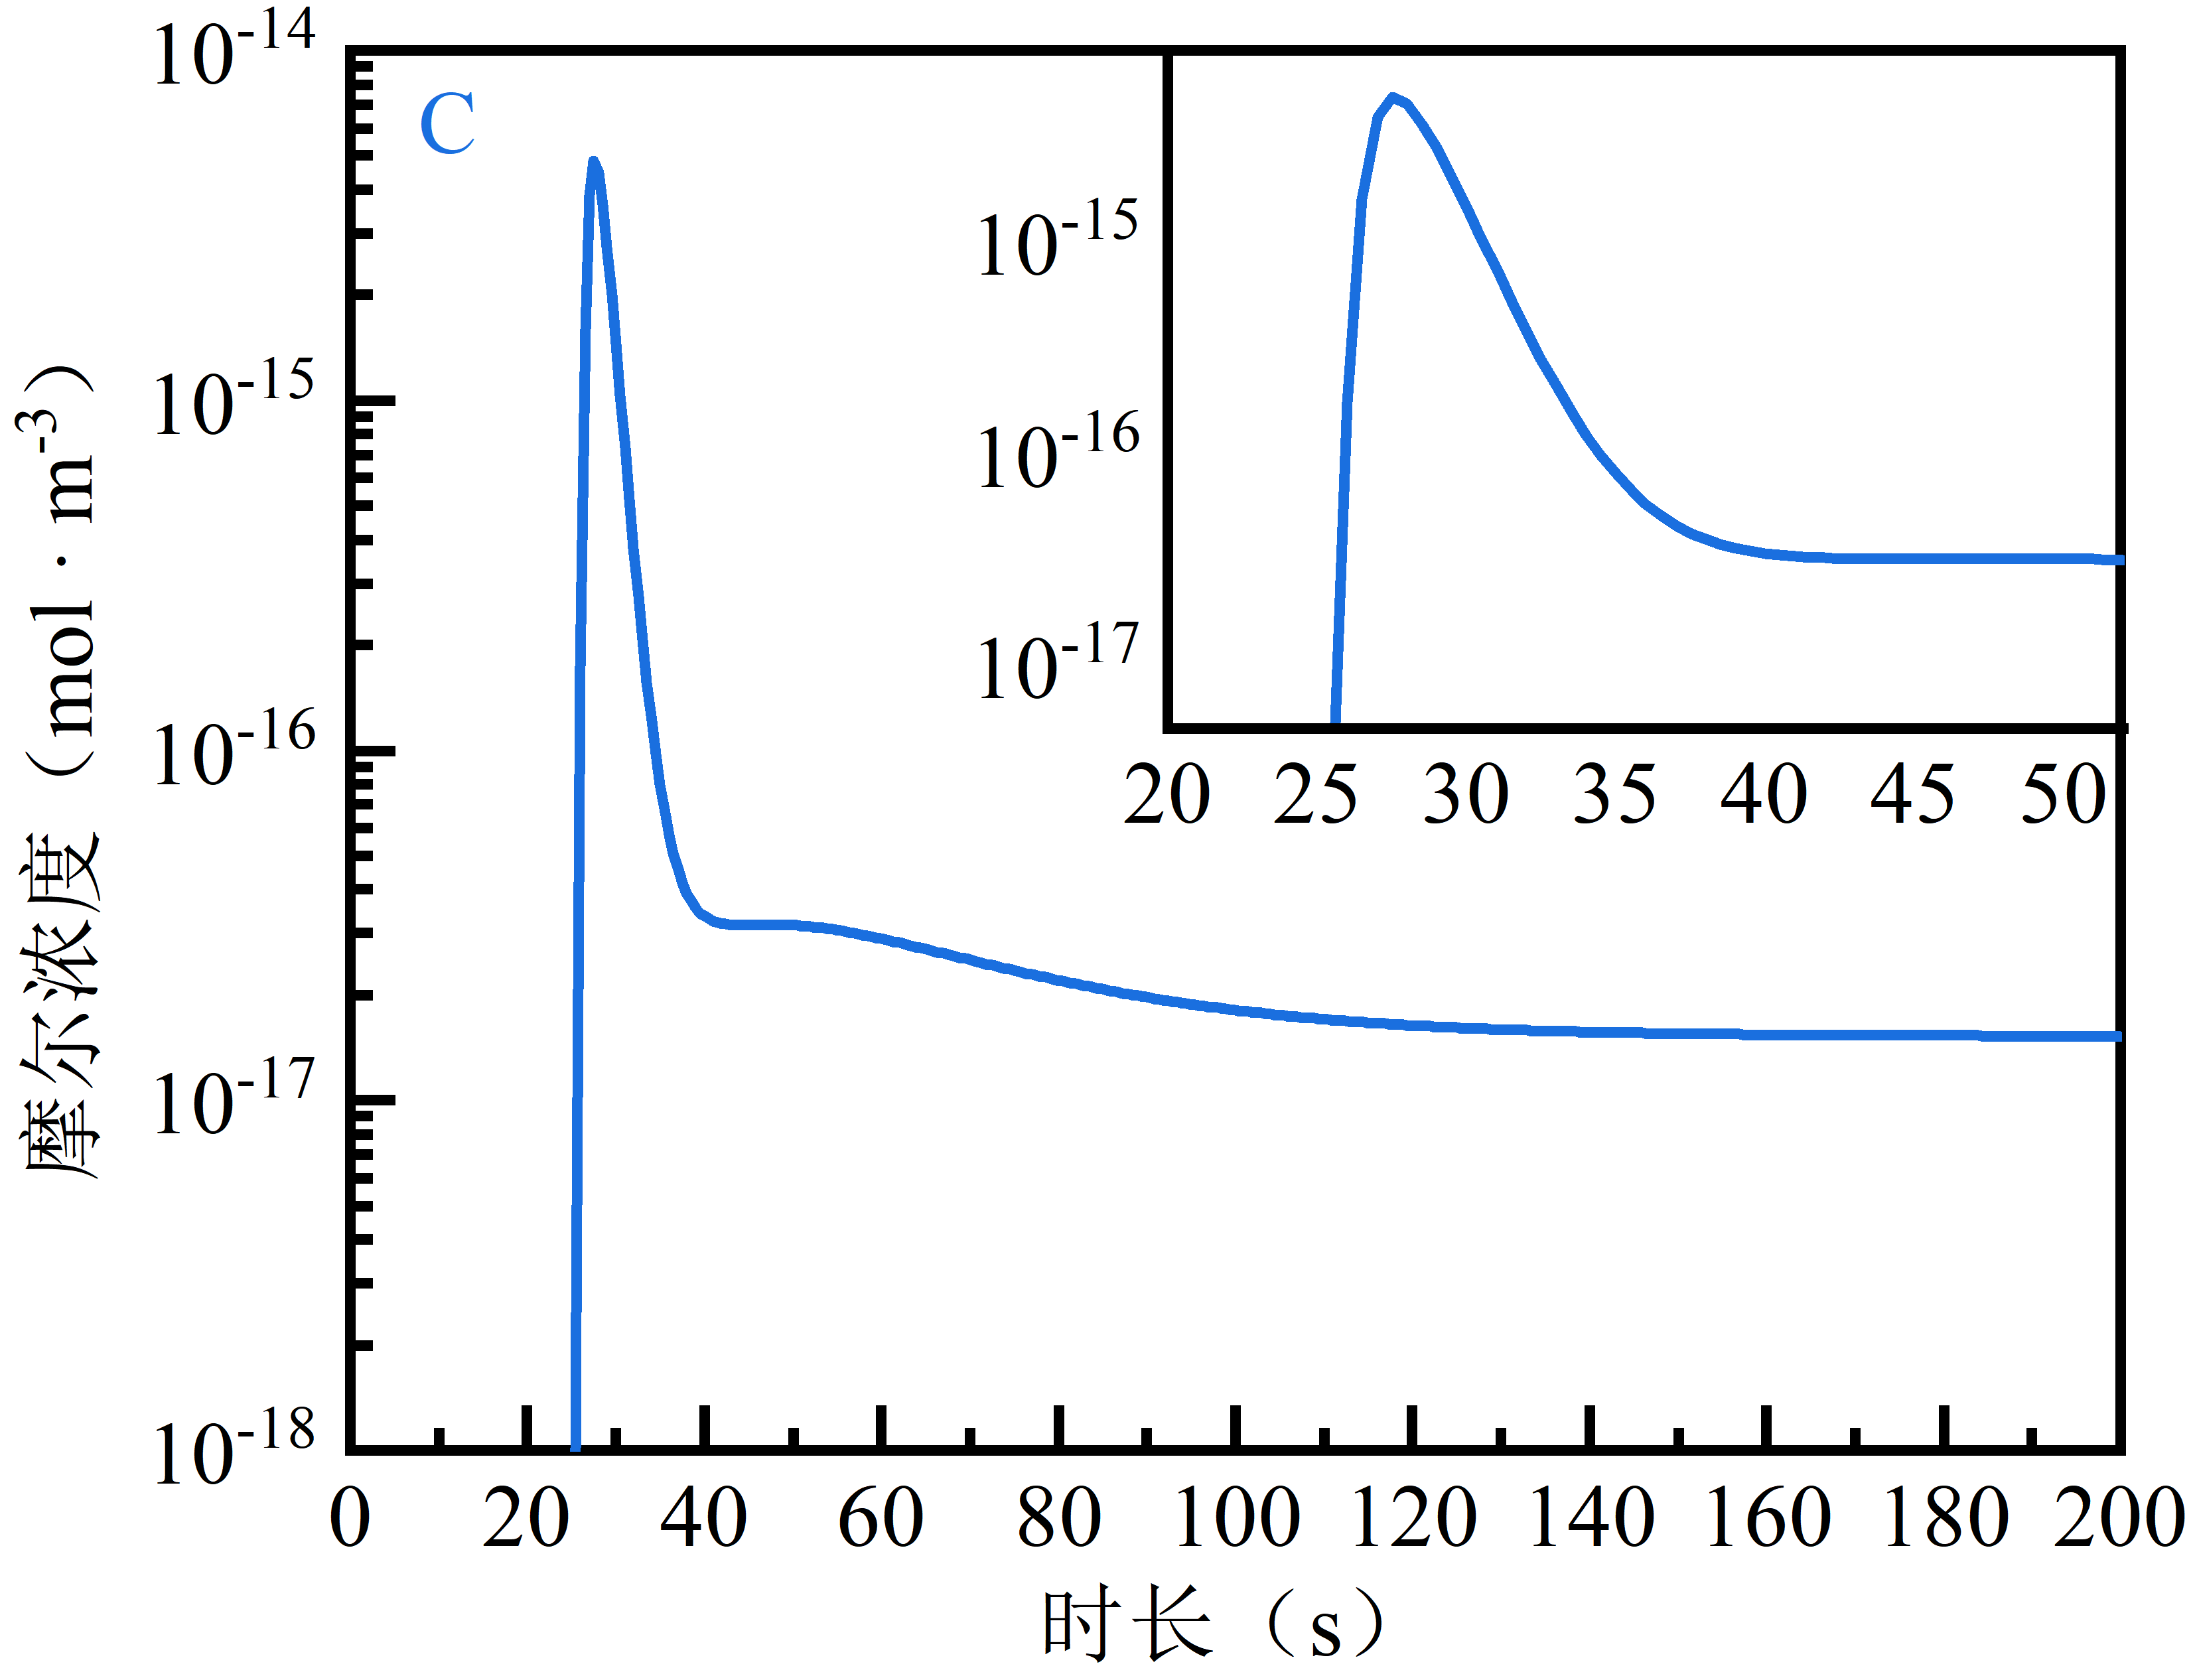
\includegraphics{pic/FLG_fluent_C_molConcen.png}
    }
    \subfloat[]{
        \label{fig:FLG_fluent_O_molConcen}
        \includegraphics{pic/FLG_fluent_O_molConcen.png}
    }\\[-0.5ex]
    \subfloat[]{
        \label{fig:FLG_fluent_O-C_ratio}
        \includegraphics{pic/FLG_fluent_O-C_ratio.png}
    }
    \caption{化学气相沉积过程中石墨烯生长位点的化学组分随时间分布的浓度变化。(a)C自由基浓度(b)O自由基浓度(c)O/C比例。
    }
    \label{fig:FLG_fluent}
\end{figure}

本论文使用反应活性最高的C自由基和O自由基作为气相中直接参与石墨烯生长和蚀刻反应的代表反应物。可以看到在常压化学气相沉积的系统内,输入氧气后大约\SI{25}{\second}之后,在石墨烯生长位点开始有明显的甲烷分解反应发生。对于C自由基而言,由于氧气参与并促进甲烷的裂解反应,C自由基的浓度极速上升,最高浓度可达$\SI{4e-15}{\mole\per\cubic\metre}$。随后由于CO、CO2等碳氧化物的生成,C自由基的浓度迅速下降,并在约第\SI{40}{\second}后C自由基的浓度稳定在$\SI{1e-17}{\mole\per\cubic\metre}$附近。而对于O自由基,情况则更为复杂。在$\SI{25}{\second}$时,氧气经过气体输运到达石墨烯生长位点,被迅速加热开始分解成为氧自由基。此时氧自由基的最高浓度最高可达$\SI{3e-11}{\mole\per\cubic\metre}$。随后由于参与甲烷裂解和与氢气的化合反应,氧自由基的浓度下降至$\SI{2e-12}{\mole\per\cubic\metre}$并在产生震荡。氧自由基浓度震荡在约$\SI{50}{\second}$处到达最高值$\SI{8e-12}{\mole\per\cubic\metre}$并逐渐回落至$\SI{3e-12}{\mole\per\cubic\metre}$。考虑到在石墨烯的生长过程中,以C自由基和O自由基为代表的活性物质对于石墨烯的生长和蚀刻作用是同时进行的,因此本论文使用O/C比来考察化学气相沉积过程中,通入氩氧混合气后生长气氛中的化合物达到平衡状态所需的时间(图\ref{fig:FLG_fluent_O-C_ratio})。可以看到,在O/C比在通入氩氧混合气的第\SI{45}{\second}后就基本趋于稳定。考虑到实验中生长多层石墨烯通常需要几十分钟乃至几个小时的时间,因此可以认为在生长气氛中引入氧气的情况下,石墨烯生长、蚀刻反应所涉及的化学气氛均已达到稳态。由此,本论文更加快速高效对生长气氛进行稳态模拟。

图\ref{fig:FLG_chemkin}展示了通入不同流量的氧气情况下石墨烯生长位点的化学组分浓度情况。为了探究前驱体中不同氧气含量对多层石墨烯生长的影响,本论文考察了氩氧混合气输入的流量从$\SI{0}{SCCM}$ 到$\SI{500}{SCCM}$时,石墨烯生长气氛中的气相化学反应情况。

\begin{figure}[htb]
    \subfloat[]{
        \label{fig:FLG_chemkin_full}
        \includegraphics[width=0.48\textwidth]{pic/FLG_chemkin_full.png}
    }
    \subfloat[]{
        \label{fig:FLG_chemkin_part}
        \includegraphics[width=0.48\textwidth]{pic/FLG_chemkin_part.png}
    }
    \caption{生长环境中化学组分浓度分布随着通入氧气流量大小的变化情况。(a)模拟中涉及的所有化合物的浓度分布情况;(b)石墨烯蚀刻物质与生长物质的浓度分布情况}
    \label{fig:FLG_chemkin}
\end{figure}

整体来看,随着通入氧气流量的上升,甲烷的裂解程度也随之上升。甲烷与氧气反应生成大量的一氧化碳和二氧化碳以及种类众多的碳氢氧化合物。而碳氢化合物的浓度随着氧气通入流量的上升呈现出先上升后下降的趋势。氢气的浓度随着更多氧气的通入逐渐下降,但活性氢原子的浓度保持在一个非常稳定的区间。
为了简化分析,在氢-氧-甲烷反应所涉及的所有物质中,本论文主要关注那些能够蚀刻石墨烯以及能够为石墨烯生长提供碳源的化合物(图\ref{fig:FLG_chemkin_part})。其中,在本章中所考虑的蚀刻物质包括氧自由基、氢氧化物和氧气,生长物质包括活性炭自由基,碳氢化合物等。

对于蚀刻物质,本论文发现随着氧气通入量的上升,O、OH以及$\cemb{HO2}$的浓度急剧上升。以氧自由基为例,活性氧自由基的浓度在氩氧混合气的输入流量为$\SI{5}{SCCM}$时约为$\SI{2e-15}{}$。在氩氧混合气的输入流量为$\SI{500}{SCCM}$时,氧自由基在气氛中的浓度提升至$\SI{3e-2}{}$,大约提升了三个数量级。而对于$\cemb{OH}$和$\cemb{HO2}$,二者的浓度随着氩氧混合气的输入流量的上升也有两到三个数量级的浓度提升。

而气氛中的生长物质随着氧气通入量的上升呈现出了了非单调的变化。氧气能够促进甲烷的裂解反应,因此气氛中的C和CH的浓度得以缓慢上升,作为甲烷裂解反应物和中间产物的$\cemb{CH4}$,$\cemb{CH3}$,$\cemb{CH2}$则缓慢下降。而其他碳氢化合物在氧气通入量逐渐上升的情况下大部分呈现出先上升后下降的浓度趋势。
\subsection{氧对多层石墨烯的穿透蚀刻机制}
\label{subsec:FLG_Oetch}

考虑到蚀刻物质中$\cemb{O}$、$\cemb{OH}$、$\cemb{HO2}$以及$\cemb{O2}$等物质都对石墨烯具有一定的蚀刻作用,且各蚀刻物质之间的浓度较为接近。为了探究石墨烯在含氧化学气相沉积环境下的蚀刻过程,本论文引入氧原子的化学势$\muO{}$来代表生长气氛中蚀刻物质的整体反应活性。因此,化学势$\muO{}$的变化范围为$\halfEOm$ 至 $\EOa$,对应于氧原子在氧气分子($\cemb{O2}$)内的能级水平和氧原子在氧自由基($\cemb{O}$)中的能级水平。随着在蚀刻石墨烯的反应中涉及的高活性蚀刻物质(如氧自由基O)浓度的上升,化学势$\muO{}$逐渐上升并接近$\EOa$,同时伴随着更多的石墨烯被蚀刻。

随后,利用密度泛函理论,在$\muO{}$的框架内计算了氧原子蚀刻石墨烯的反应能$\rm{\Delta} \it E$。
\begin{equation}
    \rm{\Delta} \it E = E_{\rm product} - E_{\rm initial} - \muO{}
\end{equation}
其中,$E_{\rm product}$和 $E_{\rm initial}$分别为各反应步骤中生成物和反应物的能量。

在以铜为衬底的化学气相沉积石墨烯生长法中,当铜的表面被单层的石墨烯覆盖满后,石墨烯多层的生长由于自限制效应而趋近于停止。此时的石墨烯-\cemb{Cu}衬底界面处存在大量的游离碳。这些游离碳在石墨烯-\cemb{Cu}衬底的界面处扩散,成核,形成少量的石墨烯多层点。从热力学的角度看,石墨烯多层点的大小于游离碳的浓度$\Cdis$处于平衡状态。当游离碳的浓度$\Cdis$上升时,处于石墨烯-\cemb{Cu}衬底的界面处的石墨烯多层点的成核密度上升、面积扩大。当游离碳的浓度$\Cdis$下降时,石墨烯多层点开始分解,面积缩小。

从密度泛函理论的计算结果来看(图\ref{fig:FLG_DFT_Oetch}),无论有无游离碳,氧原子都可以在石墨烯上吸附,并且吸附的反应能相近。对于氧气来说,由于在石墨烯上吸附需要进行裂解,因此当$\muO{}=\halfEOm$时,氧原子在界面游离碳上方的石墨烯上的吸附能约为$\SI{-0.35}{\electronvolt}$,在纯石墨烯的表面吸附能约为$\SI{-0.28}{\electronvolt}$。而对于氧自由基而言,其可以在石墨烯上直接吸附,相应的吸附步骤的反应能也会下降很多。计算显示当$\muO{}=\EOa$时,氧原子在界面游离碳上方的石墨烯上的吸附能约为$\SI{-3.63}{\electronvolt}$,在纯石墨烯上的吸附能约为$\SI{-3.56}{\electronvolt}$。

\begin{figure}[htb]
    \includegraphics{pic/FLG_DFT_Oetch.png}
    \caption{
        石墨烯多层以及石墨烯单层在含氧环境下的蚀刻。$\muO{eg}$为氧蚀刻石墨烯单层时的平衡化学势。图中,铜原子、碳原子、氧原子、氢原子分别使用橙色、灰色、红色和白色标识。
    }
    \label{fig:FLG_DFT_Oetch}
\end{figure}

氧原子吸附在石墨烯上后,和石墨烯表面的碳原子发生反应,生成非常稳定的\cemb{CO}。同时,当界面游离碳存在的时候,石墨烯上被氧原子蚀刻而成的碳空位能够被游离碳修复。这种类似于交换作用的机理使得环境中的氧原子能够通过蚀刻石墨烯单层的方式减少界面游离碳的浓度$\Cdis$,进而导致石墨烯多层点的蚀刻。计算显示,氧原子在游离碳上方的石墨烯位点蚀刻石墨烯形成\cemb{CO}的反应在所有考虑的氧原子能级$\muO{}$下都为放热反应,在$\muO{}=\halfEOm$时反应能$\rm{\Delta} \it E=\SI{-2.59}{\electronvolt}$;在$\muO{}=\EOa$时反应能$\rm{\Delta} \it E=\SI{-5.87}{\electronvolt}$。这意味着即使环境中只存在少量的氧气($\muO{} \approx \halfEOm$),生长气氛中的氧就能够通过蚀刻石墨烯单层和游离碳的交换作用对界面处的石墨烯多层进行蚀刻。

当界面处的石墨烯多层被完全蚀刻、游离碳的浓度$\Cdis$也被环境中的氧消耗至零时,氧气与石墨烯单层表面碳原子反应产生的碳空位无法被修复,在石墨烯表面产生高能态的单空位缺陷(Single vacancy, SV)。空位缺陷的产生会极高地抬升氧原子蚀刻石墨烯单层的反应能。导致的结果是只有当环境中氧原子的能级水平提高至接近氧自由基的能级$\EOa$时,蚀刻反应才能够从吸热反应变为放热反应,此时的$\muO{} \leqslant  \muO{eg}  $,才能够进一步对石墨烯单层进行蚀刻。$\muO{eg}$为氧蚀刻石墨烯单层时的平衡化学势。因此,对于石墨烯单层的蚀刻需要通入更高流量的氧气以抬高生长气氛中氧的反应活性。

\subsection{氧对多层石墨烯的穿透生长机制}
\label{subsec:Opene}
在第\ref{subsec:FLG_gasPhase}章中,本论文模拟了引入不同流量的氧气的情况下石墨烯生长位点的化合物浓度分布情况。对于生长物质,本论文发现\cemb{C2H2}分子的摩尔浓度相比于其他的生长物质的浓度高出多个数量级。因此本论文考虑将\cemb{C2H2}分子作为本章的主要研究对象,探究其对于石墨烯多层生长的影响。

首先,本论文通过密度泛函理论计算,研究\cemb{C2H2}在石墨烯表面的吸附机理(图\ref{fig:FLG_DFT_C2H2toCHO})。对于无氧生长气氛下的石墨烯,计算结果显示\cemb{C2H2}在其上的吸附反应是吸热的,吸附能为$\SI{0.11}{\electronvolt}$。
这一结果和已有的研究吻合\citing{RN248-2014}。吸热的吸附过程说明\cemb{C2H2}较难在纯石墨烯上吸附,因此也较难对石墨烯多层点的生长产生作用。在有氧的生长气氛下,在\ref{subsec:FLG_Oetch}章中,本论文已经证明了生长气氛中的氧在能量上很容易在石墨烯的表面形成吸附氧原子。当石墨烯的表面存在吸附氧原子时,进一步的计算显示气氛中的\cemb{C2H2}可以与吸附氧原子反应,在石墨烯的表面形成\cemb{C2H2O}。这一步骤的反应能下降为$\SI{-1.54}{\electronvolt}$。随后,石墨烯表面吸附的\cemb{C2H2O}能够进一步和氧反应,形成更为稳定的\cemb{C2H2O2}。\cemb{C2H2O2}在石墨烯的表面可以分解成为两个分离的\cemb{CHO},进一步降低体系能量。在反应过程中,仅有\cemb{C2H2O2}分解为石墨烯表面相邻的\cemb{CHO}(图\ref{fig:FLG_DFT_C2H2toCHO},G-2HCO)过程中有小至$\SI{0.027}{\electronvolt}$的反应能上升,其余过程均为放热反应。因此可以在生长气氛中引入氧气的情况下,气氛中的\cemb{C2H2}可以大量的在石墨烯的表面吸附、分解成为同样吸附在石墨烯表面的\cemb{CHO}。

\begin{figure}[htb]
    \includegraphics{pic/FLG_DFT_C2H2toCHO.png}
    \caption{氧辅助\cemb{C2H2}在石墨烯表面沉积、分解为\cemb{CHO}。图中,铜原子、碳原子、氧原子、氢原子分别使用橙色、灰色、红色和白色标识。}
    \label{fig:FLG_DFT_C2H2toCHO}
\end{figure}

先前的研究表明,碳自由基以及碳氢化合物(\cemb{CH_x})等物质能够通过穿透的方式,在已生长的石墨烯的下方生长石墨烯多层\citing{RN248-2014}。由于碳自由基在生长气氛中非常低的浓度,已经环境中较高的氢自由基浓度,本论文选择\cemb{CH}作为代表化合物考察碳自由基以及碳氢化合物在含氧的生长气氛下对于石墨烯的穿透生长作用。在图\ref{fig:FLG_DFT_CHpene}中,本论文计算了石墨烯表面吸附的\cemb{CH}在有氧和无氧的气氛下可能的穿透反应路线。计算结果显示在无氧的气氛下,\cemb{CH}能够很好得在石墨烯得表面吸附并且通过穿透作用形成界面游离碳原子($\rm G-C_{inter}-H$)。

\begin{figure}[htb]
    \includegraphics{pic/FLG_DFT_CHpene.png}
    \caption{含氧气氛下石墨烯表面\cemb{CH}的穿透反应过程。}
    \label{fig:FLG_DFT_CHpene}
\end{figure}

然而在有氧的情况下,在石墨烯表面吸附的\cemb{CH}会优先和氧原子结合,在石墨烯的表面形成非常稳定的\cemb{CHO}。这一反应的反应能比\cemb{CH}穿透作用的反应能低$\SI{1.03}{\electronvolt}$。氧的引入阻断了\cemb{CH}通过穿透作用生长石墨烯多层的路径,并将其变为在石墨烯表面吸附的\cemb{CHO}。而\cemb{CHO}在石墨烯表面的吸附同样也遇到了困难。计算显示由于\cemb{CHO}在石墨烯表面极高的稳定性,其进行穿透反应所需吸收的能量约为$\SI{1.05}{\electronvolt}$。即使在穿透了碳原子后,残留的\cemb{OH}官能团与气氛中的\cemb{H}反应形成水蒸气也仍旧比\cemb{CHO}在石墨烯上吸附的能量要高。

\begin{figure}[htb]
    \includegraphics{pic/FLG_DFT_Odefect.png}
    \caption{\cemb{Cu}衬底表面不同构型的氧缺陷的形成能。图中,铜原子、碳原子、氧原子、氢原子分别使用橙色、灰色、红色和白色标识。}
    \label{fig:FLG_DFT_Odefect}
\end{figure}

在含氧的生长气氛下,\cemb{Cu}衬底可能产生氧缺陷。而\cemb{Cu}衬底表面的氧缺陷可能会对\cemb{CHO}在石墨烯表面的穿透作用产生影响。为了简化后续计算,本论文首先对不同构型的氧缺陷进行形成能计算。如图\ref{fig:FLG_DFT_Odefect}所示,本论文主要考虑\cemb{Cu}衬底表面氧的三种简单的点缺陷,分别为\chinesecolon 填隙氧原子缺陷\cemb{O_{i}}、单氧原子替位缺陷\cemb{O_{Cu}}以及双氧原子替位缺陷\cemb{2O_{Cu}},其中替位缺陷均为替换单个铜原子。形成能的计算使用$E_{\rm f}=E_{\rm Cu}^{\rm defect}+{\rm n_{Cu}}E_{\rm Cu}^{\rm bulk}-\frac{1}{2}{\rm n_{O}}E_{O_{2}} - E_{\rm Cu}^{\rm perfect}$。其中$E_{\rm Cu}^{\rm defect}$和$E_{\rm Cu}^{\rm perfect}$为缺陷\cemb{Cu}衬底和完美\cemb{Cu}衬底的能量;$E_{\rm Cu}^{bulk}$和$E_{O_{2}}$为块体铜和氧气的能量;${\rm n_{Cu}}$和${\rm n_{O}}$为缺陷反应中涉及的铜原子和氧原子的数量。计算结果显示三种点缺陷的形成能均为负值,形成能最低的单氧原子替位缺陷\cemb{O_{Cu}}的计算值为$\SI{-1.21}{\electronvolt}$。因此,本论文认为在生长了石墨烯的情况下,\cemb{Cu}衬底的表面仍然很容易形成氧原子缺陷。计算得到的形成能最低的氧缺陷构型为双氧原子替位缺陷\cemb{2O_{Cu}},其形成能为$\SI{-1.94}{\electronvolt}$。在后续的计算中,本论文使用双氧原子替位缺陷\cemb{2O_{Cu}}作为主要研究对象,考察\cemb{CHO}在石墨烯表面的穿透作用。

\begin{figure}[htb]
    \includegraphics{pic/FLG_DFT_CHOpene.png}
    \caption{\cemb{Cu}衬底上不同位点的石墨烯表面吸附的\cemb{CHO}的穿透反应过程。图中,铜原子、碳原子、氧原子、氢原子分别使用橙色、灰色、红色和白色标识。穿透进入界面的游离碳原子使用蓝色标识。}
    \label{fig:FLG_DFT_CHOpene}
\end{figure}

在图\ref{fig:FLG_DFT_CHOpene}中,本论文绘制了\cemb{Cu}衬底上不同位点的石墨烯表面吸附的\cemb{CHO}的穿透反应过程,包含无氧缺陷的原生位点以及双氧原子替位缺陷\cemb{2O_{Cu}}的氧缺陷位点。对比\cemb{CHO}在铜表面原生位点的石墨烯穿透反应,铜表面的氧缺陷位点对于游离碳有更高的亲和性,消除了\cemb{CHO}穿透石墨烯的上升势。具体而言,在\cemb{Cu}衬底的氧缺陷位点,吸附在石墨烯表面的\cemb{CHO}的穿透反应能为$\SI{-1.27}{\electronvolt}$。同时,在穿透反应完成后,石墨烯上残留的\cemb{OH}官能团能与气氛中的氢反应,进一步降低体系能量并且释放处氧缺陷位点,使得\cemb{CHO}在氧缺陷位点的穿透反应能够持续不断的进行。虽然穿透反应过程中的交换作用使得原石墨烯单层表面的碳原子进入界面成为游离碳,但是\cemb{CHO}对于石墨烯表面的\cemb{Cu}衬底位点选择性穿透使得在界面处生长的石墨烯多层的碳原子主要来源于含氧气氛内的碳源。倘若穿透反应能够在石墨烯单层表面的任意位点进行,那么由于石墨烯表面吸附分子的扩散作用,穿透进入界面的游离碳并成核生长为石墨烯多层点的碳原子应该主要来自于原石墨烯单层的碳原子。因为在随机作用下,只有很少的位点会产生多层点穿透的现象。如果穿透反应对于\cemb{Cu}衬底的氧缺陷位点具有选择性,氧缺陷位点处产生的穿透通道使得大部分的穿透都在氧缺陷位点上方进行,由此会产生在石墨烯单层表面多层点穿透的情况,如此一来穿透进入界面的游离碳并成核生长为石墨烯多层点的碳原子则主要来源于生长气氛。因此,通过同位素标记法区别原石墨烯单层表面的碳原子以及含氧气氛中的碳原子,可以通过实验验证穿透的机制的选择性\citing{RN1262-2021}。

\subsection{氧辅助多层石墨烯蚀刻生长模型及模式切换相图}
综合考虑氧气的引入对于界面处石墨烯多层蚀刻和生长的影响,可以发现氧对二者均有促进作用。对于氧蚀刻反应,根据通入的氧流量的不同导致生长气氛中氧的化学势$\muO{}$的变化,本论文将蚀刻反应分为两个阶段。在第一个阶段中,只有界面处的游离碳通过与石墨烯单层的交换左右,被气氛中的氧蚀刻,导致界面游离碳的浓度$\Cdis$下降,界面石墨烯多层点减少。第二个阶段是当通入的氧流量足够高时,氧的化学势超过蚀刻石墨烯单层的平衡化学势$\muO{} \geqslant \muO{eg}$,导致石墨烯单层开始被氧蚀刻。可以将氧对石墨烯的蚀刻作用总结为以下化学表达式\chinesecolon
\begin{equation}
    \label{chemeq:OetchReaction}
    \begin{split}
        \cemb{C($\rm dis.$) + O($\rm ads.$) &->[graphene] CO(g)} \\
        \cemb{C(graphene) + O($\rm ads.$) + 2H &->[\vphantom{graphene}] CO(g) } \mbox{ only if $\muO{} \geqslant \muO{eg}$}
    \end{split}
\end{equation}
根据\ref{subsec:Opene}章,氧辅助的穿透反应可以写为\chinesecolon
\begin{align}
    \label{chemeq:OpeneReaction}
    \cemb{C2H2(g) + 2O($\rm ads.$) + 2H(g) ->[graphene][Cu oxygen defect] 2C(adlayer) + H2O(g)}
\end{align}

根据反应式\ref{chemeq:OetchReaction},可以写出理想状况下的蚀刻速率\chinesecolon
\begin{equation}
    \RateV{e}{}=\rule[0ex]{0ex}{8ex}\left\{
        \begin{array}{ll}
        \smash[t]{\overbrace{\RateK{e}{dis.}\Cdis\Oads}^{\mathclap{{\mbox{\normalsize $\RateV{e}{dis.}$}}}}} & \mbox{}  \\
        \smash[b]{\RateK{e}{dis.}\Cdis\Oads+\RateK{e}{g}\Oads} & \mbox{for $\muO{} \geqslant \muO{eq}$} 
        \end{array}\right.
        %\begin{array}{ll}\hline
        %    \rule[10ex]{1ex}{4ex}\\\hline
        %\end{array}
\end{equation}
和穿透速率\chinesecolon
\begin{equation}
    \RateV{g}{}=\RateK{g}{}\cemb{[C2H2][H2]^2}\Oads^2
\end{equation}
其中,$\RateK{e}{dis.}$、$\RateK{e}{g}$和$\RateK{g}{}$分别为游离碳蚀刻,石墨烯单层蚀刻,石墨烯多层生长的反应常数。$\Cdis$、$\cemb{[C2H2]}$、$\cemb{[H]}$和$\Oads$代表界面游离碳、$\cemb{C2H2}$化合物、$\cemb{H}$自由基以及石墨烯上吸附氧的浓度。

考虑蚀刻石墨烯多层时,氧原子对于的界面游离碳消耗\chinesecolon
\begin{equation}
    \RateV{e}{dis.}=\RateK{e}{dis.}\left(\Cdis-\RateV{e}{dis.}\right)\Oads
\end{equation}
其中,$t$为反应的时间。随着氧原子对石墨烯多层蚀刻的进行,界面游离碳逐渐被消耗,$\Cdis$的下降同时降低了石墨烯多层蚀刻反应的速率。将反应速率$\RateV{e}{dis.}$对反应时间$\ReactTime{O}{}$积分并取平均,可以得到$\ReactTime{O}{}$时间段内的氧气对游离碳的平均蚀刻反应速率\chinesecolon
\begin{equation}
    \overline{\RateV{e}{dis.}}=\frac{\int_{0}^{\ReactTime{O}{}} \RateV{e}{dis.} \,dt }{\ReactTime{O}{}}=\frac{\int_{0}^{\ReactTime{O}{}} \frac{\RateK{e}{dis.}\Cdis\Oads}{\RateK{e}{dis.}\Oads \ReactTime{}{} + 1} \,dt}{\ReactTime{O}{}}
\end{equation}
而对于生长反应,$\cemb{CHO}$在石墨烯表面的选择性吸附使得生长反应速率$\RateV{g}{}$存在一个由\cemb{Cu}衬底表面氧缺陷位点数量限制的上界。可以写出在氧缺陷处的穿透通道被饱和之前的生长反应的平均速率\chinesecolon
\begin{equation}
    \overline{\RateV{g}{}}=\frac{\int_{0}^{\ReactTime{O}{}} \RateV{g}{} \,dt }{\ReactTime{O}{}}= \frac{\int_{0}^{\ReactTime{O}{}} \RateK{g}{}\cemb{[C2H2][H2]^2}\Oads^2 \,dt }{\ReactTime{O}{}}
\end{equation}
在这些化合物的浓度中,$\cemb{[C2H2]}$和$\cemb{[H]}$本论文使用\ref{subsec:FLG_gasPhase}节中模拟出的相应化合物的稳态浓度数据。而对于$Odis$,虽然在\ref{subsec:FLG_gasPhase}章中的模拟证明生长环境中的化合物很快就达到了稳态平衡,但由于氧自由基($\cemb{O}$)较低的浓度以及氧分子($\cemb{O2}$)在石墨烯表面较低的吸附能。氧气的吸附过程可能会需要很长的一段时间才会达到饱和。为了获得$\Oads$在石墨烯多层生长过程中随时间的变化情况,本论文使用晶格随机顺序吸附模型(lattice random sequential adsorption model )对氧气以及氧原子在石墨烯表面的吸附进行模拟。

晶格随机顺序吸附模型中,本论文使用二维晶格对石墨烯进行模拟,每个晶格单元对应一个原胞大小的石墨烯。在模拟过程中,本论文考虑生长气氛中氧气分子($\cemb{O2}$)和氧自由基($\cemb{O}$)在石墨烯表面的沉积。根据密度泛函理论计算(表\ref{tab:FLG_RSA_coverage}),取$\cemb{O2}$和$\cemb{O}$在石墨烯表面吸附的饱和覆盖率分别为$1$和$1 / 4$。

\begin{table}
    \centering
    \caption{}
    \begin{tabular}{ccc}
        \toprule
        覆盖率  & $\cemb{O}$的吸附能(\si{\electronvolt}) & $\cemb{O2}$的吸附能(\si{\electronvolt}) \\
        \midrule
        1       & -4.50                                    & 0.43                                      \\
        $1 / 4$ & -4.95                                    & -0.026                                    \\
        \bottomrule
    \end{tabular}
    \label{tab:FLG_RSA_coverage}
\end{table}

同时,有别于氧自由基($\cemb{O}$)的直接吸附,氧气分子$\cemb{O2}$在石墨烯上的吸附的同时需要较高的能量进行进行裂解。本论文通过在氧气分子吸附的过程中添加$\SI{2.39}{\electronvolt}$的势垒来对这个裂解过程进行描述\citing{RN838-2012}。为了将随机吸附模拟过程中的模拟时间时长与实际通入氩氧混合气的时长进行对应,本论文根据气体的麦克斯韦-玻尔兹曼分布计算了氧自由基($\cemb{O}$)和氧气分子$\cemb{O2}$的碰撞频率,气氛中氧自由基($\cemb{O}$)和氧气分子$\cemb{O2}$的浓度也根据\ref{subsec:FLG_gasPhase}节中的模拟数据进行计算。

在图\ref{fig:FLG_RSA_Oadsorb}中,本论文计算了通入不同流量的氩氧混合气的情况下石墨烯上吸附的氧原子浓度$\Oads$随时间的变化情况。计算结果显示模拟得出的$\Oads$服从指数增长定律$\Oads\left(\it t\right)=\Oads\left(\it \infty \right)-\it De^{\it -\sigma t}$,和先前的研究一致\citing{RN837-1990,RN836-1991}。由于$\Oads$的指数形式,直接将$\Oads$带入计算$\overline{\RateV{e}{dis.}}$中的积分项为非初等函数。考虑到在实际的化学气相沉积生长过程中,氧原子在低浓度氧环境中需要花费数天甚至一个月的时间才能达到饱和吸附,远超本论文所考虑的生长时间范畴。而高浓度氧环境中会导致石墨烯被完全蚀刻,也不在本论文所关心的范围内。因此本论文将研究范围集中在氧原子吸附浓度$\Oads$的线性吸附区,这时$\Oads$相对于时间的变化关系可以简化为$\Oads\left(\it t\right)\approx \it D \sigma t$。

\begin{figure}[htb]
    \includegraphics{pic/FLG_RSA_Oadsorb.png}
    \caption{不同氩氧混合气通入流量下氧原子在石墨烯表面吸附浓度随时间的变化情况。}
    \label{fig:FLG_RSA_Oadsorb}
\end{figure}

为了确认$\Oads$线性简化是否会因为晶格随机顺序吸附模拟过程中所使用的屏蔽系数参数的变动而失效。如图\ref{fig:FLG_RSA_OabsorbPera}所示,本论文计算了在中等氧通量的情况下(氩氧混合气流量为\SI{100}{SCCM}),多种模拟参数组合下氧原子在石墨烯表面进行吸附模拟的结果。可以看到,氧气$\cemb{O2}$屏蔽系数的变化几乎无法传到至最后吸附浓度的变化。这可能是由于氧气较高的解离势垒导致尽管生长气氛中的氧气浓度较高,但氧气在石墨烯表面解离吸附在石墨烯上的能力仍然较弱。而对于氧自由基$\cemb{O}$,屏蔽系数由$1$变为$\frac{1}{2}$会降低吸附氧原子的浓度。但考虑到通常化学气相沉积法对石墨烯的生长过程通常在$\SI{10}{\hour}$以内\citing{RN1262-2021}。在这个时间范围之内,氧自由基$\cemb{O}$屏蔽系数的变化对吸附氧原子浓度的影响较小。同时也并不会影响吸附氧原子浓度在$\SI{10}{\hour}$之内随时间的线性增长关系。因此,本论文认为对氧原子吸附浓度$\Oads$使用$\Oads\left(\it t\right)\approx \it D \sigma t$进行简化并不会受模拟过程中屏蔽系数参数选取的影响。

\begin{figure}[htb]
    \includegraphics{pic/FLG_RSA_OabsorbPera.png}
    \caption{$\Oads\left(\it t\right)\approx \it D \sigma t$线性近似的晶格随机顺序吸附模拟参数稳定性测试}
    \label{fig:FLG_RSA_OabsorbPera}
\end{figure}

由此,可以计算通入$\ReactTime{O}{}$的氩氧混合气后,石墨烯的蚀刻平均速率为\chinesecolon
\begin{equation}
    \label{eq:FLG_avgVe}
    \overline{\RateV{e}{}}=
    \begin{cases}
        \frac{\Cdis_0 \log\left( 1+\RateK{e}{dis.}\Oads | \,_{t=\ReactTime{O}{}} \ReactTime{O}{} \right) }{\it 2 \ReactTime{O}{}}                                                        & \muO{} \langle \muO{eg}         \\
        \frac{\Cdis_0 \log\left( 1+\RateK{e}{dis.}\Oads | \,_{t=\ReactTime{O}{}} \ReactTime{O}{} \right) }{\it 2 \ReactTime{O}{}} + \frac{1}{2}\RateK{e}{g}\Oads| \,_{t=\ReactTime{O}{}} & \muO{} \geqslant \muO{eg}
    \end{cases}
\end{equation}
其中,界面游离碳的初始浓度$\Cdis_0$本论文取相应生长温度下碳的饱和蒸汽进行近似。$\Oads| \,_{t=\ReactTime{O}{}}$为氩氧混合气的时间为$\ReactTime{O}{}$时的石墨烯上的吸附氧原子浓度。

同样,也可以求得在\cemb{Cu}衬底氧缺陷产生的穿透通道饱和前,石墨烯的生长平均速率为\chinesecolon
\begin{equation}
    \label{eq:FLG_avgVg}
    \overline{\RateV{g}{}} =\frac{1}{3}\RateK{g}{}\cemb{[C2H2]}\cemb{[H]^2}\left(\Oads |_{\,\ReactTime{}{}=\ReactTime{O}{}} \right)
\end{equation}
式\ref{eq:FLG_avgVe}和式\ref{eq:FLG_avgVg}可以解释氧促石墨烯多层蚀刻和氧促石墨烯生长之间的反应速率的竞争对于石墨烯多层整体蚀刻、生长行为的影响。在图\ref{fig:FLG_model_avgV}中,本论文绘制了不同吸附氧原子浓度下,氧辅助石墨烯蚀刻、生长作用的平均反应速率。

\begin{figure}[htb]
    \subfloat[]{
        \includegraphics[]{pic/FLG_model_avgV.png}
        \label{fig:FLG_model_avgV}
    }
    \subfloat[]{
        \includegraphics[]{pic/FLG_model_modePhase.png}
        \label{fig:FLG_model_modePhase}
    }
    \caption{氧辅助石墨烯蚀刻、生长作用及模式切换相图。(a)氧辅助石墨烯蚀刻、生长作用的平均反应速率;(b)氧辅助石墨烯蚀刻/生长模式切换相图。其中,模式I为石墨烯多层蚀刻、模式II为石墨烯多层生长、模式III为石墨烯蚀刻(包括石墨烯多层以及石墨烯单层)}
    \label{fig:FLG_model}
\end{figure}

图中的原点代表无氧气输入的情况,此时的石墨烯呈现出自限制的生长行为。当氧气引入生长气氛时,石墨烯表面吸附的氧原子浓度$\Oads$随着氧气通入量或者含氧气氛内反应时间的上升而上升。当吸附氧原子浓度$\Oads$较低时,石墨烯多层的蚀刻速率高于石墨烯多层的生长速率,石墨烯自限制生长下的少量多层点在氧原子的蚀刻作用下逐渐减少,整体表现出石墨烯多层蚀刻的行为(模式I)。当石墨烯表面吸附氧原子的浓度$\Oads$逐渐上升时,氧原子对于石墨烯表面的蚀刻反应速率由于界面游离碳浓度$\Cdis$的下降而放缓,$\cemb{CHO}$的穿透生长反应则随着$\Oads$的上升而继续加速。此时上升的$\Oads$导致石墨烯多层的生长速率高于被界面游离碳浓度不足所限制的石墨烯多层蚀刻速率,整体展现出石墨烯多层生长的行为(模式II)。当$\Oads$的浓度上升至氧的化学势$\muO{}$超过蚀刻石墨烯单层的平衡化学势$\muO{eg}$,气氛中的氧开始直接蚀刻单层石墨烯,导致石墨烯蚀刻反应的速率大幅上升,再次超过被穿透通道饱和所限制的石墨烯多层生长速率。此时石墨烯展现出再蚀刻的行为(模式III)。在模式III中,由于较高的氧活性,不仅石墨烯多层,较为稳定的石墨烯单层也会被高反应活性的氧反应。

\section{本章小结}
在本章中,本论文利用理论计算的方法研究了化学气相沉积生长石墨烯过程中衬底形貌和生长气氛对于的石墨烯生长行为的影响。研究表明衬底表面的台阶破坏了原衬底表面的对称性,为石墨烯的成核生长提供了优先生长位点和优先生长方向,使得石墨烯有机会在多晶铜的表面实现多点定向成核生长,有利于实现大面积石墨烯单晶生长的实现。而对于生长气氛的影响,本论文的研究显示氧的引入同时促进了石墨烯多层蚀刻和多层生长的反应。而氧气对石墨烯多层的蚀刻和穿透作用的相互竞争突破了原有\cemb{Cu}衬底上石墨烯生长的自限制作用,导致了石墨烯多层交替出现蚀刻和生长的现象,有利于实现石墨烯生长过程中的层数调控。
}{}
    \IfSubStr{\MYCAPFLAG}{-4-}{\chapter{锑化铟的生长机理研究}
\section{引言}
\section{单层锑化铟生长过程及生长极性研究}
\section{双层锑化铟生长过程及生长极性研究}
\section{双层锑化铟生长及极性演化的物理机理研究}
\section{双层锑化铟生长极性相图}}{}
    \IfSubStr{\MYCAPFLAG}{-5-}{\chapter{二维材料异质结生长机理的研究}
\section{引言}
石墨烯作为经典的二维材料,由于独特的晶体结构和电子结构特性,在超导,量子计算、量子晶体管等方面具有独特的优势\citing{RN1068-2020,RN1071-2021,RN1065-2013,RN997-2007,RN1008-2015}。而要将石墨烯与现行集成电路使用的平面硅工艺兼容,需要将石墨烯转移到\cemb{SiO2}等绝缘衬底的表面。而石墨烯在\cemb{SiO2}等绝缘衬底表面通常以无序的状态存在,破碎的晶格使得石墨烯在这些绝缘衬底的表面难以完全发挥出理论上限。

而作为二维材料中的绝缘体,六方氮化硼\cemb{h-BN}在具有较大的带隙的同时也保有二维材料高质量面内结构的特点。趋近完美的二维晶体结构使得\cemb{h-BN}在禁带内具有极低的缺陷态密度以及较高的击穿电压。同时,\cemb{h-BN}与石墨烯之间的晶格失配只有\SI{2}{\percent},这使得\cemb{h-BN}非常适合搞高性能电子器件中替代\cemb{SiO2}作为石墨烯的衬底材料 \citing{RN959-2010}。这种将不同的二维材料纵向堆叠起来可以制成纵向异质结,层与层之间由较弱的范德华力或准范德华力连接。以二维材料所组成的异质结能够结合不同二维材料优异的物理特性,使得二维材料在多种新型器件中能够最大化的发挥其独特的优势。许多新奇的物理现象已经在石墨烯和\cemb{h-BN}的纵向堆叠而成的二维异质结被研究者所发现,如在外磁场下电子和磁场场强的霍夫斯塔特蝴蝶分型图像\citing{RN1286-2013, RN1287-2013, RN1285-2013}。同时,石墨烯/\cemb{h-BN}纵向二维异质结具有非常好的制备质量,石墨烯高度可调的物理特性,以及二者之间存在的周期性的摩尔超晶格。这些都使得石墨烯/\cemb{h-BN}纵向二维异质结成为了一个非常好的观测新奇量子现象的基础平台。

然而,虽然机械剥离的方式能够制备具有极高质量的石墨烯/\cemb{h-BN}纵向二维异质结,但受限于较低生产效率和高昂的合成成本,剥离的方式很难应用于大规模的二维材料的生产制备。而常用于大规模低成本制备石墨烯的化学气相沉积法通常需要\cemb{Cu}等金属衬底的催化作用的协助。由于\cemb{h-BN}对于甲烷等含碳前驱体裂解反应的催化活性远不及金属衬底,石墨烯在\cemb{h-BN}上直接生长的速率同样也远低于在金属衬底上的生长速率。因此,一些研究者试图通过增加前驱体裂解速率的方式提升纵向二维异质结的合成效率。例如,在2013年,研究者发现通过等离子体辅助的方式能够在低温的环境下在\cemb{h-BN}的表面生长石墨烯\citing{RN1289-2013}。在2015年,研究者通过添加作为气体催化剂的硅烷等方式,可以促进甲烷的裂解,提高石墨烯在\cemb{h-BN}表面的生长速率\citing{RN1059-2015}。但以上方式通常使用剥离的\cemb{h-BN}作为石墨烯的生长衬底,使用较高的生长温度或者使用等离子体辅助的方式进行生长。在这种情况下,虽然石墨烯能够在\cemb{h-BN}的表面生长,但是高温会破坏金属衬底,而\cemb{h-BN}本身的生长需要在金属衬底的表面。因此我们需要寻找到一种生长流程,使得温度维持在金属衬底能够生长\cemb{h-BN}能够的同时,尽可能的加快石墨烯在\cemb{h-BN}表面的生长速率。

在\ref{cap:CG}章中,我们构建了一种利用\cemb{Cu}蒸气近邻催化效应在\cemb{h-BN}表面直接堆叠生长石墨烯的方法。该方法利用从外缘\cemb{Cu}源处蒸发而出的\cemb{Cu}蒸气作为催化剂,在\cemb{h-BN}的表面产生对\cemb{CH4}的近邻催化效应,加速甲烷在\cemb{h-BN}表面的裂解,从而达到加速\cemb{h-BN}表面石墨烯生长的目的。利用理论计算的方法,我们证明了\cemb{Cu}蒸气从蒸发源到达\cemb{h-BN}表面并进行\cemb{CH4}裂解催化的可行性,同时给出了裂解而成的碳原子在\cemb{h-BN}表面成核生长成石墨烯的生长序列。我们认为通过这种直接堆叠生长的方法能够能够实现石墨烯/\cemb{h-BN}的双层以及多层堆叠交替大规模生长,进一步提升石墨烯/\cemb{h-BN}二维纵向异质结在高性能电子器件应用的可行性,推进石墨烯/\cemb{h-BN}二维纵向异质结的工程化和集成化。

\section{计算细节}

在本章中密度泛函理论主要使用Vienna ab-initio Simulation Package (VASP) 软件包进行计算。在密度泛函理论计算中,我们使用广义梯度近似(GGA)下的 Perdew-Burke-Ernzerhof (PBE)泛函描述电子之间的交换关联作用。平面波的截断动能取为为$\SI{500}{\electronvolt}$。为了研究\cemb{Cu}/\cemb{h-BN}衬底表面石墨烯的生长情况,我们采用切片模型并在垂直表面方向放置至少$\SI{20}{\angstrom}$的真空层以防止周期性条件相邻切片的影响。切片模型中,作为石墨烯生长衬底的\cemb{Cu}/\cemb{h-BN}包含四原子层的\cemb{Cu(111)}以及单原子层的\cemb{h-BN}。在\cemb{Cu}的表面,经过我们的计算,\cemb{h-BN}的最优堆叠方式为\cemb{N}原子位于\cemb{Cu}衬底的顶位,\cemb{B}原子位于\cemb{Cu}衬底的面心立方位(fcc site)。
在原子结构优化的计算中,力收敛条件设为$\SI{2e-2}{\electronvolt \per \angstrom}$,电子结构自洽场计算的收敛条件设为$\SI{1e-6}{\electronvolt}$。
对于碳团簇(\cemb{C_x})、石墨烯、\cemb{h-BN}、\cemb{Cu}衬底之间之间的范德瓦尔斯作用使用Grimme的DFT-D3方法进行描述,并带有Becke-Johnson阻尼作用 \citing{RN937-2010, RN938-2011}。
对于过渡态的计算,我们采用CI-NEB(Climbing Image Nudged Elastic Band)方法对始末反应状态之间的能量鞍点进行搜寻,以确定反应势垒的大小\citing{RN790-2000}。对于过渡态计算,力收敛条件设为$\SI{3e-2}{\electronvolt \per \angstrom}$。

\section{石墨烯/\cemb{h-BN}纵向二维异质结的生长机理}
    \label{cap:CG}
    \begin{figure}[htb]
        \subfloat[]{
            \centering
            \includegraphics{pic/CG_diagram_routine.png}
            \label{fig:CG_diagram_routine}
        }
        \newline
        \subfloat[]{
            \includegraphics{pic/CG_diagram_growthSketch.png}
            \label{fig:CG_diagram_growthSketch}
        }
        \caption{利用\cemb{Cu}蒸气近邻催化效应在\cemb{h-BN}表面直接堆叠生长石墨烯。(a)生长装置示意图;(b)石墨烯/\cemb{h-BN}异质结生长过程示意图}
        \label{fig:CG_diagram_CVD}
    \end{figure}

    \subsection{近邻蒸发气态\cemb{Cu}催化剂的扩散}
    
    \begin{figure}[htb]
        \includegraphics{pic/CG_diagram_FEM_structure.png}
        \caption{化学气相沉积腔体内\cemb{Cu}蒸气扩散模拟示意图。}
        \label{fig:CG_diagram_FEM_structure}
    \end{figure}

    \begin{figure}[htb]
        
    \end{figure}

    \subsection{气态\cemb{Cu}催化剂对甲烷裂解反应的催化性能}
    \subsection{\cemb{h-BN}表面石墨烯的生长演化机理}
\section{石墨烯/二硒化钒横向异质结的生长机理}
\section{总结}}{}
    \IfSubStr{\MYCAPFLAG}{-6-}{% LTeX: language=zh-CN
\chapter{总结与展望}
%//TODO 总结}{}
    \IfSubStr{\MYCAPFLAG}{-ack-}{\thesisacknowledgement
\IfSubStr{\MYANONYMOUS}{Y}{
}{
    首先我要感谢我的导师牛晓滨教授。不知不觉间在牛老师的门下已经学习和研究超过了五年时间,牛老师
    %//TODO 致谢
}
}{}
    \thesisbibliography{reference}
}


\end{document}
